\documentclass{article}

\usepackage{natbib}
\usepackage[sc]{mathpazo}
\usepackage[T1]{fontenc}
\usepackage{amsmath}
\usepackage{amsfonts}
\usepackage{amssymb}
\usepackage{graphicx}
\usepackage[onehalfspacing]{setspace}
\usepackage{color}
\usepackage[margin=.75in, tmargin=0.71in, bmargin=0.71in]{geometry}
\usepackage{url}

\usepackage{appendix}
\usepackage{hyperref}
\usepackage{xcolor}
\usepackage{todonotes}
\usepackage{booktabs}
\usepackage{lscape}
\usepackage{caption}%
\usepackage{bbm}
\usepackage{comment}

\usepackage{longtable}

\usepackage{subcaption}

\usepackage{babel}
\usepackage[autostyle, english = american]{csquotes}
\MakeOuterQuote{"}

\title{Commitment Institutions and Electoral and Political Instability: A Reduced-Form Approach}
\author{Isaac Liu\thanks{Georgetown University. Contact at \href{mailto:ijl7@georgetown.edu}{ijl7@georgetown.edu}. Acknowledgements: Prof. George Shambaugh, Prof. Joel Simmons, Dr. Greg Fischer, Joshua Levy, Tranae Hardy, Olivier Malle, Rachel Shapiro.}}
\date{Submitted as a Senior Honors Thesis in International Political Economy April 28, 2020, \newline Last Revised \today \footnote{The code for this paper, and the latest version can be found \href{https://github.com/ijyliu/Commitment_Institutions_Instability}{here}.}}

\setlength{\parindent}{0pt}
\setlength{\parskip}{0.5em}

\hypersetup{
    colorlinks=true,
    linkcolor=black,
    filecolor=black,      
    urlcolor=blue,
    citecolor=black
}

\begin{document}

	\maketitle

    \begin{abstract}
        In this paper, I take a reduced form approach to test whether the limiting institutions of central bank independence and fixed exchange rates affect electoral and more broadly political instability. This provides insight into choice among social welfare, political business cycle, and economic voting theories, which provide for numerous competing mechanisms. Differing from previous work, I consider both varieties of instability, extend analysis to various branches of government, and take care to address important endogeneity problems by using panel data and instrumental variables techniques over a wide range of countries from 1970-2012. I find suggestive evidence that de jure central bank independence and fixed rates increase instability and mixed evidence for de facto independence. In an analysis of an interaction term model, combinations of de jure CBI and fixed rates and de facto CBI and fixed rates are somewhat more destabilizing than their individual components. Overall, there is potential for serious political economy complications in the implementation of these institutions.
    \end{abstract}

    \clearpage
    \newpage

    \section*{Introduction}

    The linkage between limiting institutions such as central bank independence and electoral stability in democracies is a largely relevant debate that evades a straightforward intuitive answer. On the one hand, independent central banks are widely known as welfare-enhancing institutions which reduce inflation \citep{chicago_booth_initiative_on_global_markets_fed_2019}. This benefit comes at no long run cost to real macroeconomic variables \citep{alesina_political_1997}. It is not difficult to imagine a grateful populace consistently rewarding incumbents for better economic conditions. On the other hand, the capacity of central banks, rather than politicians to steer the economy has been assumed to have serious electoral costs in disputes such as those between President Donald Trump and Federal Reserve Chairman Jay Powell \citep{long_federal_2019}. Over time, we might expect central bank independence to repeatedly harm the electoral chances of incumbents.

    Central bank independence need not be the only economic constraint that matters for political outcomes. Fixed exchange rate regimes should also provide the same mechanism of economic policy “hand-tying” to politicians, with the outsourcing of monetary policy in open economies without capital controls \citep{fleming_domestic_1962, mundell_capital_1963}. Previous work has widely documented the importance of considering these institutions jointly \citep{bernhard_political_2002}. We thus might expect to find similar stories of fixed exchange rates affecting political and electoral stability: this is indeed the case. For example, in February 2019 the President of Cote D’Ivoire, Alassane Ouattara said that the pegged CFA franc has played a key role in stabilizing the country by helping control inflation \citep{bassompierre_ivorian_2019}. On the other hand, in Lebanon, a fixed exchange rate is considered to have led to increasing political unrest and reform pressures in the country \citep{diwan_lebanons_2020}.

    Relationships between limiting regimes and political instability also need not be limited to democracies and non-violent electoral stability. China’s tight control of the renminbi with the aim of trade promotion fits within a broader national aim of economic development to maintain domestic stability \citep{kroeber_renminbi_2011}. Contrary arguments for growing unrest and coup attempts are easily extended to current crises in semi-autocratic Turkey \citep{taner_turkish_2019} and Venezuela \citep{armas_venezuela_2019}. These nations are caught in currency crises with broad political spillovers, due in part to fixed rate mismanagement.

    Having established the relevance of the issue, in this paper I examine arguments such as these and determine whether the limiting institutions of central bank independence and fixed exchange rates affect instability. In the first section, I begin by providing an overview of competing social welfare, political business cycle, and economic voting theories and relevant literature in line with these explanations and examples.

    The presence of a robust, cross-national examination of these theories can be helpful. In the next section I provide an outline of the reduced form strategy pursued by this paper. This allows for a step back from mechanisms at work in various stages of the process to see if broad predictions align. I review similar work that has examined the reduced form relationship in democracies. General findings in this other work are that limiting institutions increase the durability of cabinets and leader tenure in open economies without capital controls (with disagreement over central bank independence), although the timing of and mechanisms affecting such effects is disputed.

    In the next section I address a critical issue, attention to which sets me apart from this past literature: any potential interventions affecting limiting regimes may be electorally motivated, made in the interests of maintaining political stability, or as a result of confounding institutions. This is a critical endogeneity problem. For example, de jure central bank independence may not be implemented, or de facto central bank independence may be eroded. Politicians may threaten to remove central bank officials from office: President Trump has considered legal options to remove Federal Reserve Chairman Powell \citep{corbett_can_2019}. In the past, such electorally motivated erosions of independence may have been successful and influential in creating low interest rate environments in the United States in the Johnson and Nixon administrations \citep{binder_trump_2019}.

    To deal with such endogeneity problems as these, I construct a design using panel data and instrumental variables techniques over a wide range of countries from 1970-2012. First, fixed effects, controls, and logit and ordinal logit models are employed to account for institutional differences between countries. With this specification, de jure central bank independence increases electoral and political instability, while de facto independence and fixed exchange rates reduce electoral turnover; fixed rates increase political instability events. Next, education and economics technical expertise provide an admittedly imperfect instrument for central bank independence, and aggregate GDP for fixed exchange rates. De jure central bank independence clearly increases electoral turnover and political instability events, and in certain specifications a similar result holds for fixed exchange rates. Finally, I observe a specification using lagged independent variables. Here I find that de jure CBI reduces head of government turnover over a long-time horizon, but also mostly increases political instability events across a variety of time scales. Contemporaneously, de facto CBI appears to be related to reduced electoral turnover, and results are mixed in other time periods, except in an ordinal logit model which shows clear instability-reducing impacts. Again, in some specifications fixed exchange rates increase electoral turnover in the mid-term. Overall, I find evidence that de jure central bank independence and fixed rates increase instability and mixed evidence leaning somewhat towards instability reduction for de facto CBI. Adding interaction terms to a lag analysis, however, I find some significance leaning towards increased instability relative to the individual inclusion of de jure CBI and fixed exchange rates and de facto CBI and fixed rates; importantly, de facto CBI and fixed rates individually decrease instability.

    Aside from testing of various codings of variables and linear and nonlinear models, I explore the instability impacts of choice among the options of the Mundell-Fleming trilemma and of democratization and its relationship to commitment institutions. I find that capital account openness and de jure CBI tend to be destabilizing choices independently and in combination, with fixed rates and de facto CBI having opposite effects, suggesting stability benefits from a Bretton Woods type system in line with earlier literature suggesting higher GDP growth. I fail to find support for hypotheses that de jure relative to de facto CBI matters more in democracies with the rule of law, and that in democracies commitment institutions have electoral rather than broader political instability impacts. Finally, I investigate divergent results based on the branch of government considered. I add in interaction terms for whether the head of government and head of state are the same individual and whether the legislature has effective power, testing theory concerning accountability of those in power in practice. It appears that the effects of commitment institutions on the Head of State variable (and in general) are often found when the Head of Government (presumably responsible for economic policy) and Head of State are the same individual, while legislature power in practice is not particularly strongly related to expected and stronger effects for commitment institutions on lower house turnover.

    I conclude with a discussion of implications and directions for future research. Theoretical work on the differing implications of de facto and de jure CBI could be insightful. Destabilizing effects of limiting regimes may add a new dimension to any normative debates over their adoption. More kinds of endogeneity should be explored in any literature on this topic. Adjustments to the methodology pursued might be useful. In an interesting case study, the Eurozone may offer a chance to compare results following varied entry dates of member nations, as well as an opportunity to examine the ideological style and type of upheaval as a result of central bank independence and a fixed exchange rate. In general, further study should be devoted to the political effects of these institutions.
    
    \section*{Theory}

    In some sense, the adjudication of the question of whether limiting institutions affect instability, and in which direction, is one between two strands of theory (some sense of this division for central banks can be found in \cite[p.212]{alesina_political_1997}). In both strands, incumbent politicians seek to deliver electoral victory or a secure hold on power. As will become clear, however, in one strand this incentive usually is aligned with the general or long-term welfare interests of the population, as adopting limiting institutions usually provides key benefits. In the other strand, however, interests are not aligned: limiting regimes prevent manipulations of the economy and are politically costly. Mechanisms from both strands are then translated into outcomes of increased or decreased stability through the economic voting literature.

    \subsection*{General Welfare Effects of Limiting Institutions}

    In the first strand lie the social welfare or planner-style implications of adopting limiting regimes. These are most often economic, but occasionally political. They affect the entire population or are focused on nationwide aggregates. They almost always rest upon the beneficial effects of commitment but may also account for a costly loss of flexibility.

    The key economic commitment benefit derived from central bank independence is the resolution of the well-known inflation time-inconsistency problem. The appointment of an independent, conservative (relative to society) central banker can improve welfare by controlling expectations of inflation \citep{rogoff_optimal_1985}, with little cost to long run real macroeconomic performance \citep{alesina_central_1993}. Along with a similar time-inconsistency inflation benefit in reducing inflation (when there are no capital controls used to maintain monetary autonomy), a fixed exchange rate may provide economic benefits such as reducing uncertainty and barriers to external trade and investment \citep{mundell_theory_1961}. It may also allow for access to foreign capital for any nations faced with an “original sin” problem, able only to borrow in foreign currency \citep{eichengreen_other_2005}.

    There may also be political benefits to limiting regimes which also increase stability and possible social welfare through increasing political efficacy. For example, monetary commitments such as central bank independence may provide information about policy for both sides of the government, increasing transparency and promoting trust \citep{bernhard_political_2002}. In terms of decisions, a fixed exchange rate may either provide a justification for hard but necessary choices or a focus for negotiations. There does not appear to be much empirical evidence to verify this part of the theory, admittedly difficult due to the abstract nature of these variables, but the theoretical logic is sound.

    However, limiting regimes may also introduce costs to valuable policy flexibility. Harmful flexibility consequences in the event of a recession may not be a major issue for independent central banking, as technocratic officials are still capable of responding. There may be problems if an inadequately flexible monetary policy rule is adopted \citep{bernanke_taylor_2015}, or central bankers are excessively conservative, as may have been the case in the early 2010s in the Eurozone \citep{krugman_opinion_2011}. But there is no reason to believe that these problems always or directly correlate with central bank independence, while the evidence clearly shows that low and stable inflation does.
    
    A more serious problem from the loss of flexibility is clear for regimes of fixed exchange rates. The fixed exchange rate precludes the free exercise of monetary and potentially fiscal policy unless capital controls are introduced \citep{fleming_domestic_1962, mundell_capital_1963}. Policy is tied to that of other nations, which may not be experiencing a recession. Adjustment may be slow and painful. \footnote{Probably the most serious other welfare loss attached to fixed exchange rates is a lack of automatic trade rebalancing through rates \citep{friedman_essays_1953}. A lack of automatic trade rebalancing is not an a priori problem for fixed rates with consequences for instability: the level of the rate may be adjusted or other trade deficit correcting measures may be taken, and there is evidence that trade is not a top issue for voters \citep{guisinger_determining_2009}. Also not a “flexibility” welfare loss per se, currency crises and speculative attacks may also be a problem of fixed rates \citep{krugman_model_1979} These situations may be mitigated, however, if IMF lending can be obtained and credible commitment to the fixed rate can be established.}
    
    Overall, net social benefits appear to outweigh the costs for limiting regimes, at least in the long run or on average, abstracting from specific incidents and problems. Commitment brings major benefits despite any costs of flexibility, especially for the case of central bank independence relative to fixed exchange rates. Arguments of net welfare drawbacks for central bank independence (to the point of advocating dependence) are especially rare, excepting complaints calling for the adoption of democratic oversight for distributional considerations or a desire for more inflation \citep{fels_downside_2016}. 
    
    The merit of fixed exchange rates appears to be far more debatable, although a large number of countries still maintain them \citep{ilzetzki_irr_2019}. Time inconsistency solutions, stable trade, and greater access to capital for “original sin” nations clearly provide serious value. If fixed rates had a net welfare cost and prevent manipulation of the economy as outlined in the section below, there would seem to be little reason left for their wide adoption, so here I maintain that they also provide a net welfare benefit.

    \subsection*{Political Business Cycle Effects of Limiting Institutions}

    The main driver of the second strand is the idea of a political business cycle: that politicians have a motivation to manipulate the economy in the short run and that institutions such as central bank independence and fixed exchange rates can limit this tendency. Motivations for political business cycles may be opportunistic (explicitly focused towards staying in office) or partisan (aimed towards implementing party policy; but as I would argue, in the process satisfying party elites and staying in power), and a wide variety of traditional and rational expectations models exist to characterize them \citep{alesina_political_1997}. In general, methods of manipulation for either of these sets of cycles may be monetary or fiscal \citep{fortunato_cabinet_2018}, and there may be some sort of substitutability between instruments in the case of limits.

    Limiting regimes should normally reduce these political business cycles. Independent Central Banking can put major limitations on incumbents’ capacity to engage in both monetary and fiscal policy business cycles. When monetary policy tools are in the hands of central bankers with non-electoral time horizons and relative freedom from political pressures, political manipulation is clearly limited. Evidence on the impact of independence on, for example, monetary, rational partisan business cycles in OECD nations have found serious reductions \citep{maloney_political_2003}.
    
    Aside from limitations on monetary policy, central bank independence may also reduce the scope for fiscal policy manipulation. In democracies with adequate protections of the rule of law, independent central banks may prefer fiscal restraint and low deficits to avoid inflation, any may threaten interest rate increases or denial of credit to enforce it. This pattern has been found to hold particularly true in non-election years under left government tenure \citep{bodea_central_2017}.
    
    Fixed exchange rates are also likely to put major constraints on monetary policy. Again, citing the Mundell-Fleming trilemma, in an open economy without capital controls, fixed rates preclude independent monetary policy. They effectively represent an outsourcing of what was once a means to manipulate the economy. Policy is subject to the maintenance of the rate, rather than electoral opportunism or partisanship. \footnote{One notable manner of escaping a fixed exchange rate constraint may come from the synchronization of electoral cycles identified as a growing trend worldwide \citep{tufte_political_1980}. A synchronized electoral cycle may allow a nations monetary policy controlled from abroad through a pegged rate to again align with domestic political interests, provided that the nation which the currency is pegged to experiences its own political business cycles, perhaps due to factors such as a lack of central bank independence}
    
    Adopting a fixed exchange rate may, on the other hand, allow for a loosening of fiscal policy. A fixed exchange rate may increase confidence in a nation’s ability to repay external debt which is not denominated in its own currency, opening access to vast amounts of foreign capital. This may be particularly important for any nations faced with an “original sin” problem, able only to borrow in foreign currency \citep{eichengreen_other_2005}. The theoretical effect of fixed rates on overall manipulation is hence unclear.
    
    However, the evidence for a net limiting impact of both CBI and fixed rates on political business cycles through these theoretical mechanisms seems to be convincing. For OECD nations from the 1960s to the 1980s, evidence suggests that both regimes, at least at levels above their average values, reduce cyclical (opportunistic) behavior in both time-series and cross-sectional analysis, although the effect of fixed rates is of net small and difficult to detect as significant \citep{clark_international_1998}. This occurs for variables of both output and employment, potentially affected by both monetary and fiscal policy.

    \subsection*{Economic Voting}

    Central to the implications of the strands above is the literature on economic voting. There must be a mechanism in place through which voters respond to economic variables and manipulation, and politicians should be aware of this mechanism. Voters may be concerned with their own status (pocketbook concerned) or with the overall economy (sociotropic), and retrospective (backward-looking) or prospective (forward-looking).

    A review of the literature generally reveals that economic voting exists, which means that political business cycles are in fact plausible. In particular, this economic voting is sociotropic and retrospective, with the exception of cases when an incumbent is not running, when voting is more prospective \citep{lewis-beck_economic_2000,nadeau_national_2001}.\footnote{Argument for more widespread prospective voting in the literature does appear to be common, so the simplifying consensus here is perhaps overstated. US Index of Consumer Sentiment data seems to indicate that presidential approval ratings, for example, can be fully accounted for by prospective evaluations and forecasting \citep{mackuen_peasants_1992}.}  I abstract from these cases by noting that prospective evaluations are still likely to be informed by past performance. \footnote{In future work, I aim to more fully account for prospective cases by locating and making use of data on whether incumbents are running.}

    Politicians also appear to be aware of economic voting, creating the appropriate motivations for welfare enhancing or manipulative behavior. There is at least good anecdotal evidence on this point. \footnote{To my knowledge, there has been no statistical or cross-national analysis of politician beliefs on the importance of the economy to voters, or on which economic variables they think matter to voters.} In the US, for example, statistical studies were actually commissioned by top government officials which found a clear responsiveness of vote shares to economic conditions as early as the 1970s \citep{tufte_political_1980}. Perhaps the most famous articulation of awareness was that of the 1992 U.S. presidential campaign, when Bill Clinton’s chief strategist James Carville put up a sign in campaign headquarters that read: “It’s the economy, stupid!” \citep{anderson_end_2007}

    With a sociotropic, mostly retrospective, and well-known model of economic voting in place, we can now move through to evaluate the electoral implications of limiting institutions through each strand of mechanisms. The implied instability consequences of welfare effects of limiting institutions fit well with findings of mostly retrospective and sociotropic voting. Voters reflect on their net improved present condition under the limiting regimes. They are glad to see that society is permanently better off with the new institutions, facing a better output-inflation tradeoff, stable trade, and greater political efficacy along with other net benefits despite some loss of flexibility. As a next step, a happy society and electorate consistently rewards elected officials for maintaining these good conditions and institutions.

    Within the political business cycle strand, with sociotropic and mostly retrospective voting, the general effect seems to be that of increased instability from limiting institutions due to decreased manipulation. If political business cycles are opportunistic or directly driven by short-term desire to stay in office, economic voting predictions of the consequences of limits on manipulation are relatively straightforward. The incumbent would like to create socially desired short-term conditions for variables such as low inflation and unemployment but cannot do so. \footnote{In rational opportunistic or partisan models covered in detail in earlier drafts of this paper, a similar mechanism is at play as incumbents try to demonstrate competence to society or the party but cannot do so under limits.} Retrospective voters may then explicitly punish them at the polls by voting for an opponent. This increases instability.

    In a partisan model, the only real change to the consequences of failure to deliver on preferences comes from the fact that optimal levels of economic variables are not socially uniform, but instead specific to parties and groups of heterogenous agents. Again, the incumbent tries to satisfy their party optimums but cannot do so. Now retrospective elites or party voters are not adequately satisfied. They need not vote for opponents; however, a loss of turnout or participation may be enough to inflict electoral damage, a case especially strong if there is some cost to voting \citep{downs_economic_1957}. Here again, limiting institutions in the political business cycle model are likely to increase instability.

    \subsection*{Varieties of Instability}

    To account for potentially more autocratic situations or even democratic situations between elections, it should be noted that in this paper I generalize the same ideas about economic voting to situations when voting may not necessarily be fair and competitive. In other cases, disaffection may be expressed more loosely in “political”, rather than “electoral” instability or turnover terms (perhaps reaching the level of violence). Welfare benefits of commitment institutions may limit the results of this disaffection. Likewise, political business cycles need not necessarily adhere to an electoral calendar but may also manifest as efforts by leaders to head off rebellion in general by placating the population. Restrictions on business cycles are then likely to further instability.

    Electoral instability in terms of the turnover of government officials may also be expressed through changes in a variety of branches. For this project, I consider two forms of the elected executive: the head of government and the head of state. The head of government is the individual leading policy making in a nation, while the head of state is the symbolic and ceremonial leader, often with importance for diplomatic relations. These may be the same individual, such as the President of the United States, or different individuals such as the President and Chancellor of Germany. I also consider the lower house of the legislature (given that upper house data for bicameral nations is not currently available). This is typically a more directly elected body with control over revenue and general legislation.

    \section*{A Reduced-Form Approach}

    The key merit in the reduced form approach to the question is that of the ability to take a step back from literature on specific mechanisms mentioned above. It could be the case that certain mechanisms are true and others false: partisan or opportunistic political business cycles, or action and limits through only fiscal or monetary policy. Mechanisms could be further tangled between each other in complex causal relationships such as substitutions between regimes (central banks and fixed rates) or kinds of policy. The reduced form approach allows for overall focus on whether the regimes weigh on instability, adjudicating whether basic intuitions are reasonable.

	\begin{figure}[h!]
		\centering
		\caption{Effects of Limiting Institutions on Instability}
			\begin{subfigure}{.5\textwidth}
				\centering
				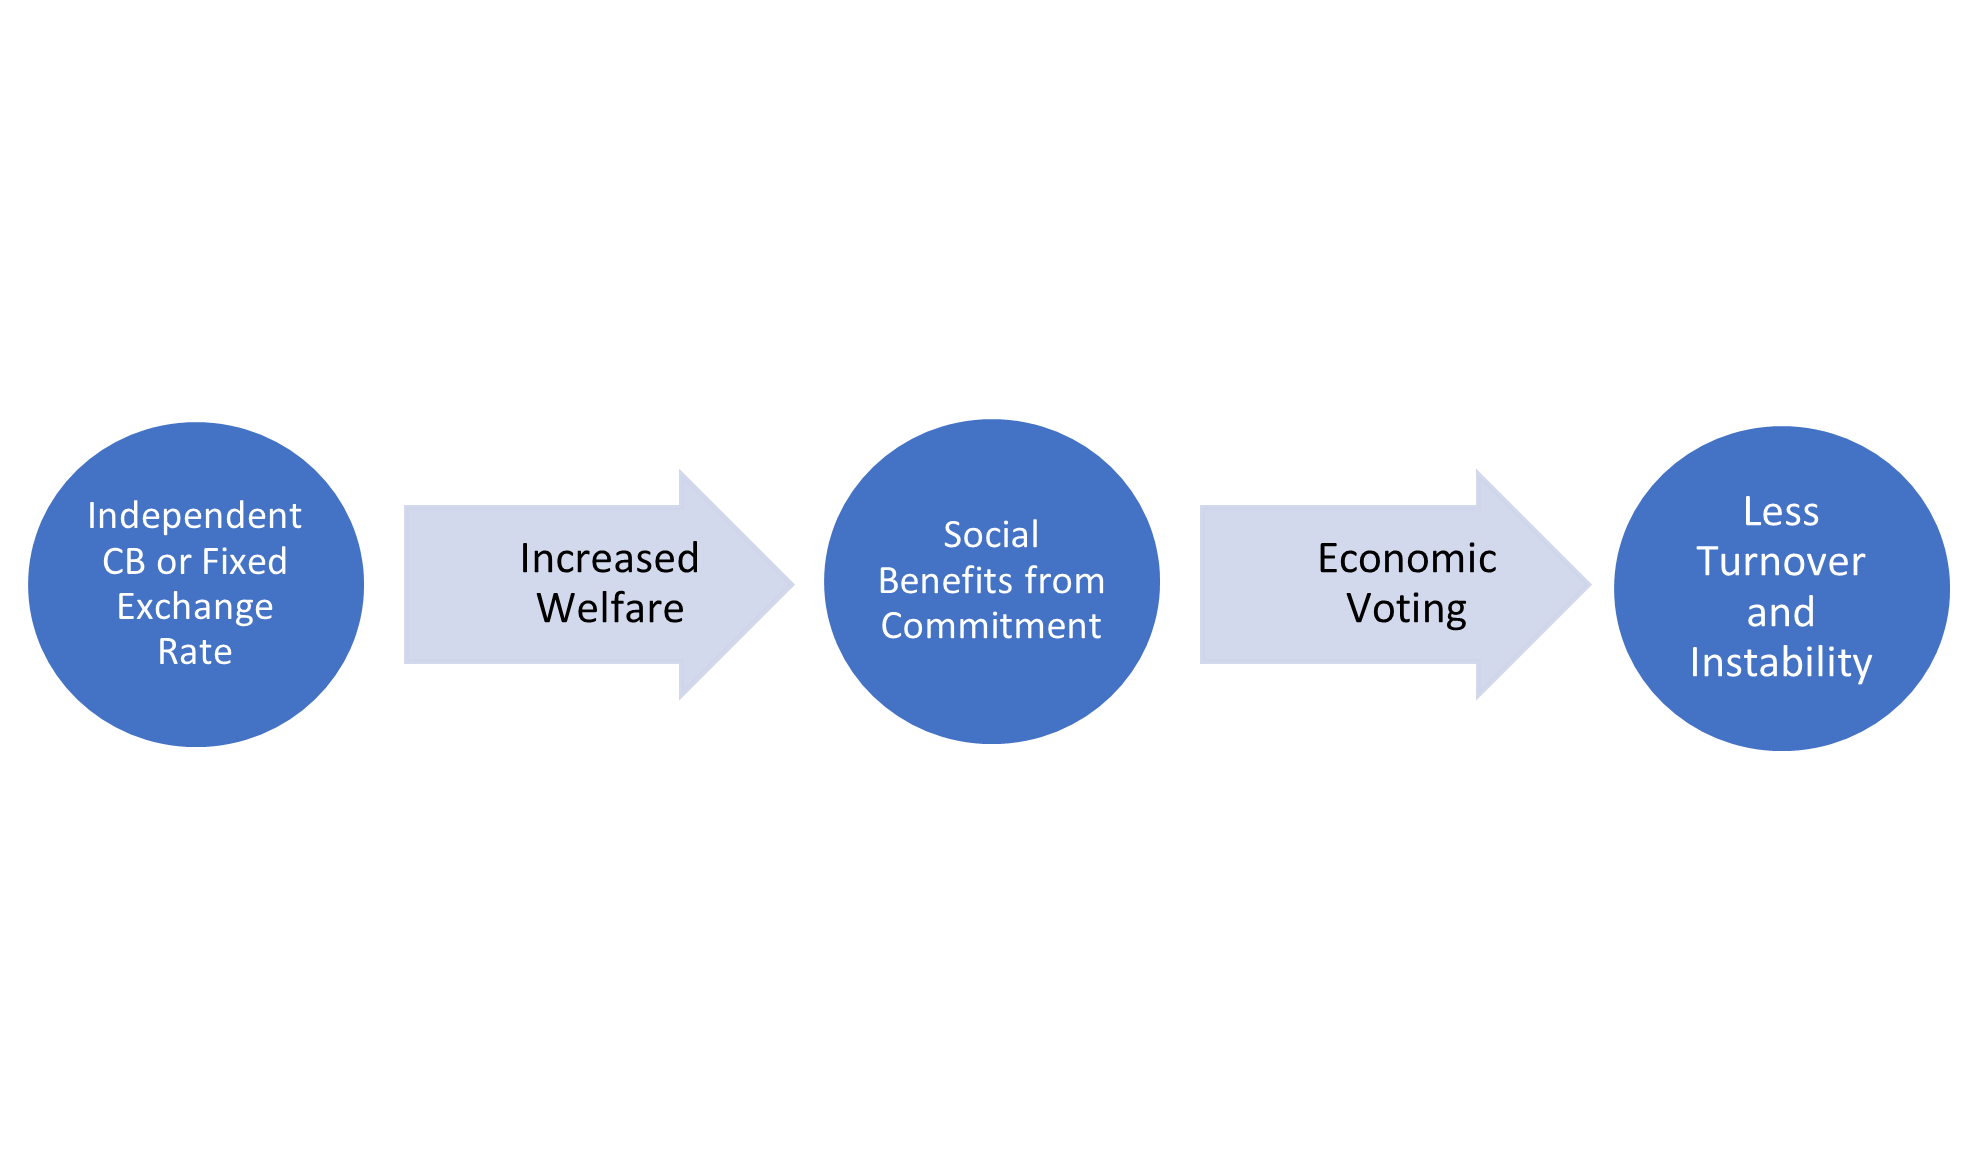
\includegraphics[width=\linewidth,keepaspectratio=true]{../../Output/Figures/Social_Welfare_Model.png}
				\caption{Welfare Model}
			\end{subfigure}
            \vskip\baselineskip
			\begin{subfigure}{.5\textwidth}
				\centering
				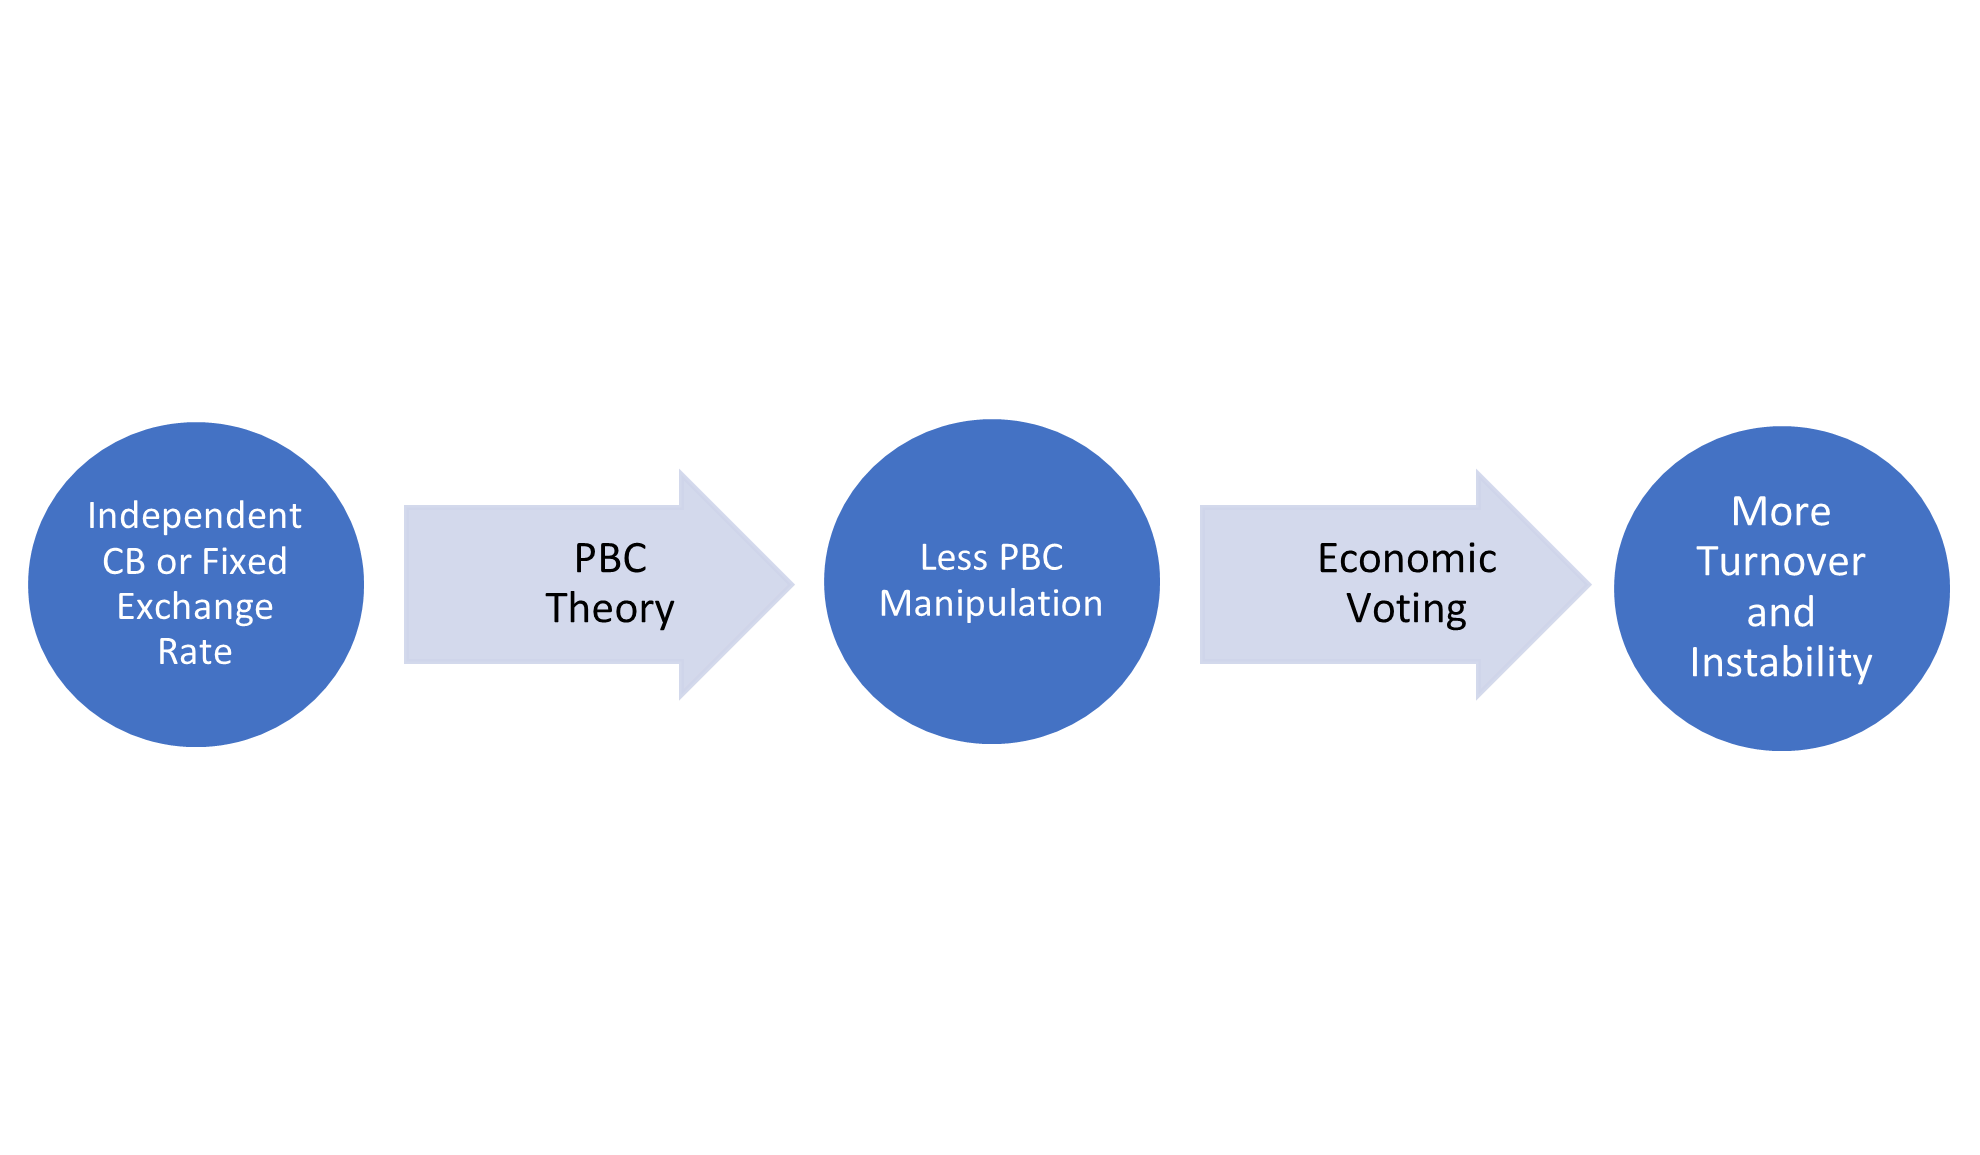
\includegraphics[width=\linewidth,keepaspectratio=true]{../../Output/Figures/Political_Business_Cycle_Model.png}
				\caption{Political Business Cycle Model}
			\end{subfigure}
	\end{figure}

    Similar work has examined the use of monetary commitments to increase the durability of cabinets (as a share of maximum legal duration) in the face of growing international economic openness and globalization for 16 parliamentary democracies from 1972 to 1998 \citep{bernhard_political_2002-1}. These commitments are hypothesized to allow for the management of diverse interests and improve policy efficacy by providing information, justifying hard decisions, and providing a focus for negotiations, in line with the social welfare strand. In OLS results, independent central banks were found to increase cabinet duration by nearly three months, and fixed exchange rates by about five. Coalition governments saw stronger benefits, while openness to trade had a mixed impact on the scale of effects. 
    
    A focus on parliamentary democracies only as in Bernhard and Leblang unfortunately weakens the use of this paper in the overall judgement of political business cycles and impacts on voter welfare. Cabinet durability may be more a function of party and coalition system dynamics, rather than actual voter stances in many situations. The nature of endogenous elections accounted for may also introduce dynamics not found elsewhere. In my work, I instead focus on a broader range of political systems.
    
    Probably the most similar work to mine I have located on the reduced form relationship between limiting institutions and political survival has made use of a Cox-proportional hazard model for leader tenure in 19 OECD countries during the recent era of high capital mobility \citep{clark_monetary_2013}. \footnote{As a key difference, in my further explorations section, I employ data on capital controls and openness rather than making any temporal assumptions of this nature.} Included were controls for endogenous elections, single-party majority governments, and the number of electoral districts (to represent fractionalization). The hypotheses that under capital mobility, fixed exchange rates (with independent central banks) and dependent central banks increased leader survival after 7 years in office were seemingly confirmed. \footnote{The assumption here appears to be that fixed exchange rates actually free up access to fiscal policy manipulation (with increased access to capital), which is an acceptance of the counterargument mentioned near the end of the section “Political Business Cycle Effects of Limiting institutions” at the end of this paper. This seems to contradict the evidence arguing fixed rates reduce manipulation at least for output and unemployment \citep{clark_international_1998}, although (note again) results on this topic are tentative (correctly signed but not very significant) and there may be other means of fiscal policy manipulation such as transfers not as easily detectable in the aggregate.} This is claimed to provide some evidence against political business cycle and economic voting literatures, at least in the early part of incumbent terms: outside means such as diversionary war or other factors such as resignations are said to be likely more important in determining leader survival.

    \section*{Endogeneity Issues}

    Importantly, I argue that both works on the topic are faced with potential endogeneity problems. Several institutional variables accounted for do give a good sense of changes relative to “normal” cabinet duration induced by limiting institutions. These include controls for fractionalization, polarization, and endogenous electoral timing, items which I seek to replicate using country fixed effects. But the provided OLS and hazard regressions do not rule out the potential that the choice of commitment institutions and their de facto strength may be dependent on politics and stability considerations specifically, nor do they capture other potential confounders such as federalism or corporatism. \footnote{Cox hazard models in particular may be vulnerable to endogeneity if there is rate dependence with time varying covariates \citep{goodliffe_hazards_2003}. Decisions of political leaders may be affected by cabinet duration. To some extent, the inclusion of lags in regressions may mitigate such issues, and I deploy this solution for this project, but given that the question of correct specification is critical, I also use instrumental variables methods.}

    There is every reason to believe that central bank independence is a political question. For example, there are a wide variety of areas on which responsibilities between governments and central bankers can be divided where political considerations may come into play, such as the setting of broader targets and objectives and the appointment of central bank officials \citep{eijffinger_political_1996}. 
    
    This point is especially salient in the consideration of de jure and de facto independence. De jure, or statutory independence tends to be rather fixed over time \citep{garriga_central_2016}, meaning that it tends to be based on a single set of decisions when relevant legal measures are passed, perhaps limiting political considerations to that period. But the matter of de facto central bank independence is far more often political. This can be seen in the current example of the Trump administration given earlier: regardless of the law, political interference and threats are very much possible. Political actors may be heterogenous in the value they place on independence, as outcry to these events indicated.
   
    Some authors have argued that de jure independence is not important in developing nations or non-democracies. In terms of predicting the impact on average inflation rates, turnover of bank executives is superior to de jure independence in a number of countries \citep{cukierman_measuring_1992}. Justification for the fact that independence seems to create fiscal restraint only in democratic and rule of law countries comes from the fact that, due to political circumstances, these countries have de facto and not just de jure independence \citep{bodea_central_2017}.
   
    If politics in general may influence the level of central bank independence, then it is not a far leap to presume that stability or instability considerations influencing political decisions have an impact; we should be wary of endogeneity problems in this reduced form examination. The literature in fact documents specific models and mechanisms for this impact \citep{eijffinger_political_1996}. Instability may lead to a more independent central bank as incumbents seek to limit the range of options available to opponents (there are case study examples of this \citep{goodman_politics_1991}). On the other hand, increased instability may inspire a greater need to make use of the political business cycle to remain in office, reducing independence.
   
    Attempts have been made to unify these theories by noting that in nations with high degrees of consensus or low polarization, instability increases independence, with the reverse true in nations with low consensus. Tests find expected signs when using appropriate measures of legal central bank independence and instability for each type of nation (party instability in high consensus nations, regime instability in low) (Cukierman 1992). Later work focused on de jure independence and found effects only for high-level changes in regimes and coups \citep{cukierman_political_1995,haan_central_1996}. Finally, other checks using the frequency of government changes and significant government changes and a variety of central bank autonomy measures find mixed results and negative or null results \citep{de_haan_variation_1995}.
   
    Aside from these valid concerns that instability affects independence, there are other channels through which independence and turnover may be related: competing mechanisms relative to political business cycle theory and economic voting. Here I cover several such confounding institutional mechanisms: checks and balances (including bicameralism, federalism, and judicial review) and corporatism.
   
    Various components of systems of checks and balances within government have been shown to be positively associated with central bank independence. De jure independence has been shown to be far higher in OECD nations with two legislative decision making bodies and a veto system \citep{moser_checks_1999}. De facto independence in terms of the relationship between statutory independence and actual inflation outcomes has also been demonstrated to be stronger in nations with such checks and balances.
   
    As another example, there is significant evidence suggesting a relationship between central bank independence and federalism \citep{lijphart_patterns_2012}. A correlation of 0.60, significant at the 1\% level was demonstrated, particularly strong in the period before the 1990s, when independent central banking was “internationalized.” Notable examples of the pairing included Germany, the US, and Canada. Aside from the association between bicameralism and federalism, subnational authorities may assert their own policy preferences on economic issues, providing another check. Overall, Lipjhart also places the power of judicial review on the same “unitary-federal” dimension as central bank independence, also demonstrating its linkage. Thus, we have one final link between a check and central bank independence.
   
    It is also easy to see how checks and balances could be related to instability. One potential mechanism for this can be constructed from a model of retrospective voting similar to those considered earlier. Voters expect their elected officials to deliver on general, and not just economic policy promises. When checks and balances prevent officials from doing so, they may explicitly punish them at the polls or more simply fail to turnout and participate. As this mechanism occurs across governments, instability increases. Hence, checks and balances increase central bank independence but also instability directly, leading to a potential overestimate of effects.
   
    Coordinated and centralized wage bargaining, often referred to as corporatism, may increase control of inflation. This can provide a helpful complement motivating central bank independence, as committed central bank reactions to negotiation developments improve outcomes \citep{hall_mixed_1998}. Inflation expectations are also controlled, allowing for lower unemployment and inflation. A key example can be found in the remarkable success of the German Bundesbank before European integration. With this realization, one might expect these institutions of corporatism and independence to go together, although the evidence is not entirely clear on this account \citep{lijphart_patterns_2012}.
   
    Corporatist institutions may also be linked to lower electoral or political instability. Centralizing demands for negotiation may lead to less need for strike, open protest, or other action. Since corporatism might be linked to central bank independence and decreased instability, we may obtain an underestimate of the effects of independence on turnover.
   
    Exchange rate regimes are also likely to face endogeneity problems. As an example of an endogeneity problem, electoral instability is also likely to affect choices of rate regimes in democracies. One mechanism functions through political economy desires to balance incumbent rent extraction and reelection. When there is no approaching election, the incumbent seeks to extract rents from a strong tradeable goods sector helped by a competitive and flexible exchange rate. Non-tradeable workers prefer fixed rates which minimize inflation, and due to numerical superiority, their preferences are critical when an election approaches. Overall, frequent elections and the associated higher levels of electoral instability should support the maintenance of a fixed exchange rate.
   
    This argument found support with the usage of hazard models to analyze the duration dependence of Latin American exchange rate arrangements from 1960 to 1999. Results showed that impending election increases the conditional likelihood of staying on a peg by about 8 percent, while the aftershock of an election conversely increases the conditional probability of going off a peg by 4 percent \citep{blomberg_sustaining_2005}.
   
    Under certain conditions, the probability of a change in cabinet may also fuel speculative attacks which precede changes in exchange rates \citep{leblang_politics_2000}. Market expectations about changes in government policy here are critical. Research seems to suggest that the link is causal, although effects are small: two standard deviations of increase in political uncertainty increased the chance of speculative attack by only about two percent.
   
    Several factors may also have an impact on exchange rate regimes and instability. For example, different groups in society are likely to have different rate preferences. Firms involved in cross-border trade and investment are likely to support a fixed exchange rate, especially if currency options markets are insufficiently developed \citep{frieden_theory_2014}. These are likely to include specialized exporters, multinationals, and international banks. On the other hand, standardized exporters and tradeable producers are more likely to prefer flexible rates (often depreciated in reality). For both kinds of exporters, the tradeoff between stability offered by fixed rates and gains from depreciation is critical.
   
    Institutional factors provide the link between groups with the most power (and hence control over rate regimes) and political stability. Federalism and bicameralism again provide good examples. Populations of commodities producers such as farmers may be widely geographically dispersed, increasing their power in federal systems and in bicameral ones when an upper house is geographically districted. This increases the likelihood of a flexible rate. For reasons similar to those above, these checks on power may also imply increased instability. Hence the potential for fixed rates to decrease stability is likely to be overstated.
   
    Another example of potential confounding factors comes directly from the “original sin” argument \citep{eichengreen_other_2005}. Original sin nations (and firms and citizens in them) are likely to have large amounts of foreign currency debt, providing incentives for the maintenance of a fixed rate regime. These nations may also be subject to increased economic instability, justifying their original sin nature. This may be tied to or spill over into political or electoral instability. Again, the potential for fixed rates to decrease stability is likely overstated.
    
    \section*{Methodology}

    When using the reduced form approach, I implement several measures to account for these sources of endogeneity across both types of limiting regimes. First, I aim to use panel data from a broad range of countries over the period considered. The implementation of fixed effects with panel data may help deal with some of the confounders mentioned. Institutions such as bicameralism or other institutional variables may be constant for many nations over the period studied. In the same vein lie issues such as the “regular” length or terms of office for leaders in a nation noted in previous work \citep{bernhard_political_2002-1}. Panel data should also allow me to conduct my analysis using the appropriate number of lags to help deal with endogeneity.

    To deal with the potential endogeneity problem of political interference specifically, I test measures of de facto independence in terms of the irregular turnover of central bank governors as an independent variable in regressions. These events represent times when a governor is forced out on a time scale not consistent with the legally mandated or suggested schedule. Due to concerns of a “bad control” problem and the concern of introducing bias, given that de jure central bank independence is likely to affect de facto independence, I consider the cases of each variable in separate regressions.

    As an additional measure to deal with endogeneity, I also pursue an instrumental variables approach for central bank independence. Past literature has used instruments such as governance indices from the World Bank’s Aggregate Governance Indicators Dataset on national measures such as “rule of law” and “voice and accountability” \citep{crowe_central_2008}. These measures are clearly inadequate for the study of turnover and instability, presenting poor exclusion restrictions as they could be directly related to dependent variables.

    Therefore, I introduce a novel instrument for central bank independence in the form of tertiary education enrollment rates. \footnote{For this instrument, I use percentage values (enrollment rates) rather than raw numbers of graduates (although these values could be easily calculated in future). It could be argued that a country only needs a certain raw number of tertiary graduates before it can run an independent central bank. However, it may also be the case that more populous nations may require more central bank staff. This may be particularly relevant when one considers the example of the system of regional Federal Reserve Banks in the United States. The use of percentages also better accounts for the actual availability of graduates for service to the central bank. Tertiary graduates are assumed to have a choice between occupations in the government or private sector; raw numbers do not necessarily mean more expertise available, and a large educated share of the populace provides a better proxy.} The theoretical justification for the first stage of this instrument is as follows: a requisite level of expertise is needed for the controlled, technocratic administration of monetary policy. For example, this may involve the presence of PhD economics graduates. Higher levels of education may proxy or at least signal for competence; they at least indicate higher private labor market returns \citep{card_causal_1999}. Outside of central bank operations, education may be necessary for the understanding of time inconsistency problems at the core of arguments for independence.

    Of course, tertiary education enrollment may not be fully necessary or the only path to central bank independence. Here I abstract from technical assistance programs provided by the IMF and other organizations that may substitute for homegrown capacity achieved through education. Nevertheless, levels of education are likely to have an influence.

    In terms of an exclusion restriction, past work has exogenously tied, for example, primary education to social-political instability in simultaneous equations models; results may be similar for tertiary education \citep{alesina_income_1993}. Theoretically, a connection can be explained by aspirations of modernization through education exceeding the reality of economic development, causing a peak of instability when measures such as literacy rates, for example, are at intermediate levels. Educated and unemployed students can form a serious source of instability, seen clearly in cases such as Korea in the 1960s \citep[p.48]{huntington_political_1976}.

    I argue that such an exclusion restriction between tertiary education and instability remains defensible, however. First, statistical evidence for the connection of the education, development gaps, and political violence appears to be somewhat weak, holding in some specific cases but not in a broad cross-national model \citep{hibbs_jr_mass_1973}. Next, the case applies to imbalances, not levels of education more generally. We need not assume that on developmental paths towards higher education a gap between education and development always emerges at similar stages. Finally, in this paper, I will seek to use the instrument in the analysis of electoral turnover rather than political instability. Above theories seem to apply more to revolutionary activity.

    The strongest counter case in democracies might come from an observation of events such as the Vietnam War protests in the United States or other movements of educated students with electoral implications. While an increase in education might cause animosity against certain policies or leaders particularly unpopular with key groups however, it is not clear that over the span of the full period this directly and generally translates into more frequent electoral turnover and alterations of power. Another notable counterpoint is that of the youth share of the vote in national elections. In Western democracies, youth turnout is low compared to other groups, a fact compounded by aging populations and small shares of populations (mean of about 20\%) \citep{institute_for_democracy_and_electoral_assistance_youth_1999}. Overall, for the period studied, the percentage of college graduates in national vote totals is likely to be small.

    In the case that the restriction remains unconvincing, I also make use of an alternative instrument more specific than tertiary education. My original ideal instrument in the vein of technical expertise was the number or amount of Economics graduates (or PhD graduates) in a country. Unfortunately, data on this subject specifically was lacking. Nevertheless, the OECD does have some data from 2005 on for the percentage of all graduates in the more general fields of business and social sciences \citep{oecd_students_2020}. I multiply these values by total population graduation rates to get a sense of the total availability of experts in these fields as a share of population. I believe that while the technical expertise first stage mechanism remains in place, the argument for an exclusion restriction between the amount of graduates in these fields and electoral instability is stronger.

    The adaptation of an instrument for fixed exchange rates is somewhat more challenging. One good predictor of exchange rate regimes is inflation \citep{mauro_long-run_2002}, but here we run into a clear problem, as inflation is already a potential mechanism in the link between fixed rates and instability that we seek to consider. Other candidates may be a nation’s level of development, trading share with primary partners, terms of trade volatility, and various capital mobility indicators, but relationships with fixed rates appear to be unclear and disputed in the data. 

    As a solution, I adopt one of the best predictors found in the literature: absolute size of the national economy in terms of GDP or GNI. Large economies are associated with floating rate regimes in nearly all studies \citep{mauro_long-run_2002}. The explanation comes from optimum currency area literature. For these nations, the importance of a stable currency for trade is less important relative to the ability to control their own large domestic economy through monetary policy- reliance on external nations is minimal. The exclusion restriction for large economies is certainly not perfect, but it should at least be noted that economic size escapes any explanations for instability or turnover based purely on levels of economic development; here I do not use per capita values.

    \section*{Data}

    \subsection*{Dependent Variables}

    I obtain data on most of my dependent variables from the compiled Varieties of Democracy Dataset \citep{michael_coppedge_v-dem_2020}. V-Dem contains hundreds of variables, including numerous ones useful for noting electoral and political instability of various degrees and the tracking of institutional characteristics. The V-Dem project is a collaboration of dozens of experts and researchers from around the world which produces reliable data with a consistent methodology, and in this case, I mostly rely on factual data about events.

    The most important dependent variables I make use of are V-Dem’s event variables for electorally-induced changes in the head of government, head of state, and control of the lower chamber of the legislature for a country in each election year. This allows for an event-based analysis of turnover with varying levels of central bank independence and fixed rates. For the head of government and head of state variables, an election year coding of 0 indicates the same individual, a coding of 1 represents a different individual but of the same party, and a coding of 2 indicates a change of individual and party. In parliamentary systems, changes within coalitions are coded as 1, and new party rule is coded as a 2. For the lower chamber variable, a coding of 0 indicates a majority comprised of the same parties, a coding of 1 indicates the assumption of a minority party or change of leadership in the same coalition or in a coalition with some new and old parties, and a coding of 2 indicates a loss of a majority or plurality dominant position.
    
    Regarding V-Dem turnover data, it is important to note that for these three variables, a coding of 0 is also used in any year in which there is an election of some sort for the head of government or head of state, but these positions are not affected by the elections. In the United Kingdom, where the head of state (monarch) is never affected by an election, there remains a head of state coding of 0 on head of state turnover for every parliamentary election date. This is a potential source of bias and inaccuracy, particularly if monarchy or asynchronous elections for the head of state and government (as in Germany) are related to instability of any kind. However, in this case, the usage of country fixed effects and instrumental variables should resolve the problem, since electoral scheduling and impacts on offices should be constant institutional variables for the time studied, and since it is difficult to see any relation with GDP or education. \footnote{If data on constitutions and sufficient resources for correction were available, country coding could be adjusted to correct the situation by marking as missing years when a position did not have an election.}
    
    For more profound political instability, I make use of V-Dem’s event variables for attempted coups, civil wars, and internal conflict. For the simplification of regressions, I combine these variables into a single binary variable representing the fact that one of these events happened in a year (a coding of 1 versus 0). Like most of the V-Dem variables, the source variables are available for a wide variety of countries and years, representing thousands of individual observations.
    
    Finally, for an idea of the overall perception of political instability and violence without a breakdown into components over a more continuous scale, I also make use of the World Bank Governance Indicators on Political Stability and Absence of Violence, a constructed index for 1996-2018 in over 200 countries \citep{world_bank_world_2020}. The variable PV.EST follows a standard normal distribution. Lower values represent lower values for good governance variables- in this case, a lower value means more political instability. The index ranges from about -2.5 to 2.5. The index is compiled from country expert ratings which provide some measure or reliability: as will become clear it generally produces results in line with V-Dem’s factual event reporting.

    \subsection*{Independent Variables}

    To measure Central Bank Independence I use the components of the Cukierman, Webb, and Neyapti \citep{cukierman_measuring_1992} index as compiled by Garriga \citep{garriga_central_2016}. The CWN index is a standard largely trusted in literature on Central Bank Independence. It gives a good sense of the statutory or de jure central bank independence and is based on legal characteristics concerning terms of office of governors, resolution of conflict, objectives, and limitations on lending to the public sector. Garriga provides data from 1970-2012 for 187 countries.

    For de facto central bank independence, I use information about turnover rates for central bank governors. Past literature has found governor turnover to be related to at least inflation, particularly in developing countries \citep{cukierman_measuring_1992}. Dreher et al. compile information on changes in central bank governors for almost all countries in the world from 1970 \citep{dreher_when_2010}. Of interest is the indicator for irregular central bank governor turnover, which occurs when a governor departs before the end of their expected legal term. In other cases, use is made of the time in office variable, which counts number of years the current governor has served in each year.

    For data on exchange rate regimes, I use annual classifications developed by Ilzetzki, Reinhart, and Rogoff which cover 1946-2016 for 194 countries \citep{ilzetzki_irr_2019}. These are de facto values compiled by experts in the field. Here the distinction between de jure and de facto arrangements does not appear to be necessary: rate regimes do not have the same kind of rule of law or governance basis, so the de facto values are likely enough. I use their fine classification coding, which allows for nuanced analysis with 16 different categories or rate regimes. In binary cases, values of 1-8 are treated as fixed and 9-14 as floating. I also check usage of numeric values on the entire scale.

    For the gross tertiary education enrollment instrumental variable, I use global indicators data published by the World Bank (in turn collected from the UNESCO Institute for Statistics) \citep{world_bank_school_2020}. As mentioned above, for the secondary instrument of social sciences and business graduates I make use of OECD data on shares of graduates for particular fields provided from 2005-2017 \citep{oecd_students_2020}. The restriction to OECD nations is not a major problem, as these make up a good representative share of worldwide democracies, but the short time horizon leaves some reason for concern, particularly given the emergence of the Eurozone and relevant monetary uniformity.

    As my imperfect instrument for exchange rate regime, I use an estimation of aggregate GDP from V-dem, obtained by multiplying GDP per capita (Maddison’s estimate) in current US dollars by the level of population \citep{michael_coppedge_v-dem_2020}. As a robustness check, I also use 2011 PPP adjusted GDP figures directly from the World Bank in some regressions \citep{world_bank_gdp_2020}.

    Finally, for most of my institutional controls I check variables built into the Varieties of Democracy Dataset. These are indices constructed based on expert opinion. Although many institutional characteristics are likely absorbed as country fixed effects for the period studied, I still seek to test significance making use of available data tracking changes over time where possible. One such included variable is the Inter-American Development Bank’s constructed index on checks and balances and other governmental stability measures for over 180 countries from 1975-2017 \citep{scartascini_database_2018}. For the evaluation of federalism, I use built-in V-Dem data on whether regional governments exist and their degrees of relative power. For a measure of corporatism there is no variable in V-Dem, but here I use Visser’s index compiled with methodology which seems to be in line with the literature \citep{kenworthy_quantitative_2003,visser_ictwss_2019}.

    A table of summary statistics for all variables is available in the appendix (Table \ref*{sumstatsAll}).    

    \section*{Results}

    All the following regressions were performed with robust and clustered standard errors, with the former proving useful for OLS models, and the latter for fixed effects panel regressions at the country level. Levels of variation in stability or number of turnover events are likely to vary considerably across the sample \citep{bernhard_political_2002-1}.

    Selected results for the full sample tests are shown in the first group of tables. In OLS regression (Table \ref*{multIndOLSDJ}), de jure Central Bank Independence is associated with increased turnover of the Head of Government by 0.321 points on V Dem’s two point turnover scale- indicating, for example, a roughly 30\% percent higher chance that either a new individual or new party occupies the Head of Government position when Central Bank Independence moves from its sample minimum to sample maximum (Cukierman index value 0 to 1). Importantly, in a country and year fixed effects regression (Table \ref*{multIndFEDJ}), this relationship loses significance.

    \begin{table}[htbp]\centering
\def\sym#1{\ifmmode^{#1}\else\(^{#1}\)\fi}
\caption{De Jure CBI, Ordinary Least Squares with Robust Standard Errors \label{multIndOLSDJ}}
\begin{tabular}{l*{5}{c}}
\toprule
                &\multicolumn{1}{c}{(1)}&\multicolumn{1}{c}{(2)}&\multicolumn{1}{c}{(3)}&\multicolumn{1}{c}{(4)}&\multicolumn{1}{c}{(5)}\\
                &\multicolumn{1}{c}{Head of Govt. Turnover}&\multicolumn{1}{c}{Head of State Turnover}&\multicolumn{1}{c}{Lower House Turnover}&\multicolumn{1}{c}{WB Political Stability (Absence of Violence)}&\multicolumn{1}{c}{Instability Event Indicator}\\
\midrule
De Jure CBI (CNW&    0.321\sym{*}  &    0.648\sym{***}&    0.587\sym{***}&    0.308\sym{**} &    0.488\sym{***}\\
Index)          &   (2.51)         &   (5.96)         &   (5.01)         &   (2.80)         &  (11.69)         \\
\addlinespace
Exchange Rate   &  -0.0147\sym{**} &  -0.0130\sym{**} & -0.00280         &   0.0347\sym{***}& -0.00292         \\
Classification (RR inverted, higher = more fixed)&  (-2.61)         &  (-2.61)         &  (-0.49)         &   (6.45)         &  (-1.74)         \\
\addlinespace
Constant        &    0.617\sym{***}&    0.157\sym{**} &    0.413\sym{***}&   -0.598\sym{***}&    0.193\sym{***}\\
                &   (8.50)         &   (2.70)         &   (6.19)         &  (-7.54)         &   (8.73)         \\
\midrule
Observations    &     1399         &     1399         &     1141         &     2141         &     4207         \\
\bottomrule
\multicolumn{6}{l}{\footnotesize \textit{t} statistics in parentheses}\\
\multicolumn{6}{l}{\footnotesize \sym{*} \(p<0.05\), \sym{**} \(p<0.01\), \sym{***} \(p<0.001\)}\\
\end{tabular}
\end{table}

    \begin{table}[htbp]\centering
\def\sym#1{\ifmmode^{#1}\else\(^{#1}\)\fi}
\caption{De Facto CBI, Ordinary Least Squares with Robust Standard Errors \label{multIndOLSDF}}
\begin{tabular}{l*{5}{c}}
\toprule
                                        &\multicolumn{1}{c}{(1)}&\multicolumn{1}{c}{(2)}&\multicolumn{1}{c}{(3)}&\multicolumn{1}{c}{(4)}&\multicolumn{1}{c}{(5)}\\
                                        &\multicolumn{1}{c}{HoG Turnover}&\multicolumn{1}{c}{HoS Turnover}&\multicolumn{1}{c}{L. H. Turnover}&\multicolumn{1}{c}{WB Pol. Stability}&\multicolumn{1}{c}{Instab. Event}\\
\midrule
De facto CBI                            &   -0.200\sym{**} &   -0.206\sym{***}&   -0.227\sym{***}&    0.145\sym{*}  &   0.0397         \\
                                        &  (-2.99)         &  (-3.43)         &  (-3.33)         &   (2.28)         &   (1.87)         \\
\addlinespace
Fixed Rate                              & -0.00757         & -0.00722         &  0.00980         &   0.0306\sym{***}&  0.00354\sym{*}  \\
                                        &  (-1.47)         &  (-1.62)         &   (1.84)         &   (6.49)         &   (2.10)         \\
\addlinespace
Constant                                &    0.893\sym{***}&    0.619\sym{***}&    0.837\sym{***}&   -0.504\sym{***}&    0.320\sym{***}\\
                                        &  (12.23)         &   (9.17)         &  (11.44)         &  (-6.78)         &  (14.40)         \\
\midrule
Observations                            &     1651         &     1651         &     1334         &     2669         &     4491         \\
\bottomrule
\multicolumn{6}{l}{\footnotesize \textit{t} statistics in parentheses}\\
\multicolumn{6}{l}{\footnotesize \sym{*} \(p<0.05\), \sym{**} \(p<0.01\), \sym{***} \(p<0.001\)}\\
\end{tabular}
\end{table}

    {
\def\sym#1{\ifmmode^{#1}\else\(^{#1}\)\fi}
\begin{tabular}{l*{5}{c}}
\hline\hline
                &\multicolumn{1}{c}{(1)}&\multicolumn{1}{c}{(2)}&\multicolumn{1}{c}{(3)}&\multicolumn{1}{c}{(4)}&\multicolumn{1}{c}{(5)}\\
                &\multicolumn{1}{c}{Head of Govt. Turnover}&\multicolumn{1}{c}{Head of State Turnover}&\multicolumn{1}{c}{Lower House Turnover}&\multicolumn{1}{c}{WB Political Stability (Absence of Violence)}&\multicolumn{1}{c}{Instability Event Indicator}\\
\hline
De Jure CBI (CNW Index)&    0.276         &    0.303\sym{*}  &    0.389\sym{*}  &   -0.417\sym{**} &    1.000\sym{***}\\
                &   (1.44)         &   (2.30)         &   (1.99)         &  (-2.75)         &  (11.15)         \\
[1em]
Exchange Rate Classification (RR inverted, higher = more fixed)&  -0.0120         &  -0.0207\sym{***}& -0.00615         &   0.0106         &  0.00690         \\
                &  (-1.61)         &  (-3.45)         &  (-0.71)         &   (1.69)         &   (1.33)         \\
[1em]
Constant        &    0.618\sym{***}&    0.390\sym{***}&    0.535\sym{***}&   0.0283         &   -0.113\sym{*}  \\
                &   (6.15)         &   (5.43)         &   (4.99)         &   (0.31)         &  (-2.20)         \\
\hline
Observations    &     1399         &     1399         &     1141         &     2141         &     4207         \\
\hline\hline
\multicolumn{6}{l}{\footnotesize \textit{t} statistics in parentheses}\\
\multicolumn{6}{l}{\footnotesize \sym{*} \(p<0.05\), \sym{**} \(p<0.01\), \sym{***} \(p<0.001\)}\\
\end{tabular}
}

    \begin{table}[htbp]\centering
\def\sym#1{\ifmmode^{#1}\else\(^{#1}\)\fi}
\caption{De Facto CBI, Fixed Effects Regression with Clustered Standard Errors \label{multIndFEDF}}
\begin{tabular}{l*{5}{c}}
\hline\hline
                    &\multicolumn{1}{c}{(1)}&\multicolumn{1}{c}{(2)}&\multicolumn{1}{c}{(3)}&\multicolumn{1}{c}{(4)}&\multicolumn{1}{c}{(5)}\\
                    &\multicolumn{1}{c}{Head of Govt. Turnover}&\multicolumn{1}{c}{Head of State Turnover}&\multicolumn{1}{c}{Lower House Turnover}&\multicolumn{1}{c}{WB Political Stability (Absence of Violence)}&\multicolumn{1}{c}{Instability Event Indicator}\\
\hline
(Lack of) Irregular &      -0.117         &     -0.0512         &      -0.211\sym{**} &     0.00955         &      0.0244         \\
CB Governor Turnover (higher = more de facto CBI)&     (-1.68)         &     (-0.81)         &     (-2.81)         &      (0.36)         &      (1.36)         \\
[1em]
Exchange Rate       &    -0.00548         &     -0.0117\sym{*}  &     0.00444         &      0.0153\sym{*}  &      0.0128\sym{**} \\
Classification (RR inverted, higher = more fixed)&     (-0.82)         &     (-2.06)         &      (0.53)         &      (2.08)         &      (2.73)         \\
[1em]
Constant            &       0.805\sym{***}&       0.521\sym{***}&       0.865\sym{***}&      -0.247\sym{***}&       0.261\sym{***}\\
                    &      (9.91)         &      (7.75)         &      (9.43)         &     (-3.54)         &      (6.77)         \\
\hline
Observations        &        1651         &        1651         &        1334         &        2669         &        4491         \\
\hline\hline
\multicolumn{6}{l}{\footnotesize \textit{t} statistics in parentheses}\\
\multicolumn{6}{l}{\footnotesize \sym{*} \(p<0.05\), \sym{**} \(p<0.01\), \sym{***} \(p<0.001\)}\\
\end{tabular}
\end{table}


    Although a result does hold in the OLS case, a lack of irregular turnover (representing high de facto CBI) does not significantly relate to electoral change in the head of government in fixed effect regressions (t-values are somewhat borderline). In regressions with just this variable and no other independent variables, however, (see Appendix Table \ref*{irregtdHOGalone}) de facto independence is negatively related to change in the head of government with a coefficient of about 22\%. Supporting this result is evidence that long time in office for central bank governors is negatively related to election turnover (Appendix Table \ref{timeinoffHOGalone}). In OLS regressions with de jure CBI (Table \ref*{multIndOLSDJ}), a Reinhart-Rogoff exchange rate regime classification closer to a fixed rate seems to be associated with less change in the head of government, but again the result does not hold with fixed effects or when included in the same regression as de facto central bank independence (Table \ref{multIndOLSDF}).

    Stronger results, however, emerge with the positive relationship between turnover of the head of state, rather than the head of government and the de jure CBI index and a negative relationship between HOS turnover and fixed exchange rates. This relationship holds even in fixed effects models (Table \ref*{multIndFEDJ}). But in this case, de facto central bank independence has a far weaker relationship (Table \ref*{multIndFEDF}). Finally, turning away from the executive branch and towards the legislative branch by examining changes in the lower house also reveals strong results for a positive relationship between de jure independence and electoral changes, and a negative relationship between de facto independence and changes. Exchange rate regimes are insignificant.

    For the full sample it is also instructive to test the relationship between independence and measures of more profound political instability. The World Bank Governance Indicator for Political Violence is positively related to de jure central bank independence in OLS regression (meaning it is associated with less instability), but the coefficient becomes negative with the inclusion of country and year fixed effects (meaning independence is associated with more instability). Such a result suggests the importance of accounting for possible confounders in literature on this topic, and it is particularly insightful given that it holds even on the restricted timescale for which World Bank data is available. De facto independence and a more fixed exchange rate are associated with stability mostly in OLS regressions. However, a fixed rate also increases political stability in a fixed effects regression with de facto independence and when considered individually (Appendix Table \ref*{WBratesalone}). Destabilizing events such as civil wars, coups, and internal conflict are positively related to de jure independence and fixed rates in both OLS and Fixed Effects regressions. When considered individually (Appendix Table \ref*{instabRRalone}) or with de facto CBI, fixed exchange rates still tend to increase the probability of instability events in a fixed effects regression, somewhat contradicting results for the World Bank index.

    Overall, the full sample results lend credence to a political business cycle type model for de jure central bank independence, holding most strongly for results on the turnover of heads of state and in the lower chamber. Higher de jure independence is also clearly related to more political instability. The picture for de facto central bank independence through a lack of irregular governor turnover, however, appears to be different. This institution seems to be related to lower electoral turnover in the admittedly few significant regressions, so we can say that de facto central bank independence might be governed by welfare effects, rather than political business cycle considerations. A reducing sign is clear for electoral instability and fixed rates, but signs on political instability are unclear.
    
    Although such results do hint at the significance and sign of relevant variables, effect sizes are difficult to interpret. Electoral turnover may also be treated as an ordinal outcome, rather than continuous and linear variable. Tables \ref{ordLogDJ} and \ref{ordLogDF}  display the mean marginal effects results (without constants) for an ordinal panel logit with clustered standard errors but random effects (fixed effects are unavailable due to current limitations); for coefficients, see Appendix Table \ref{coeffordLogDJ} and \ref{coeffordLogDF}. Significance results are generally unchanged, except for exchange rate regime which is now just barely significant for turnover in the head of government. For both kinds of CBI, impacts are substantial, with a change from sample minimum to maximum levels being associated with large (up to double digit) swings in probability. Considering the granularity of exchange rate classifications, ranging from 1 to 16 on Reinhart and Rogoff’s Index, these effects are of a similar scale.

    {
\def\sym#1{\ifmmode^{#1}\else\(^{#1}\)\fi}
\begin{tabular*}{\linewidth}{@{\hskip\tabcolsep\extracolsep\fill}l*{3}{c}}
\hline\hline
                &\multicolumn{1}{c}{(1)}&\multicolumn{1}{c}{(2)}&\multicolumn{1}{c}{(3)}\\
                &\multicolumn{1}{c}{}&\multicolumn{1}{c}{}&\multicolumn{1}{c}{}\\
\hline
De Jure CBI (CNW Index)&                  &                  &                  \\
1.\_predict      &   -0.146         &   -0.208\sym{***}&   -0.316\sym{***}\\
                &  (-1.93)         &  (-3.54)         &  (-3.65)         \\
[1em]
2.\_predict      &   0.0152         &   0.0390\sym{***}&   0.0980\sym{**} \\
                &   (1.80)         &   (3.32)         &   (3.21)         \\
[1em]
3.\_predict      &    0.131         &    0.169\sym{***}&    0.218\sym{***}\\
                &   (1.93)         &   (3.47)         &   (3.68)         \\
\hline
Exchange Rate Classification (RR inverted, higher = more fixed)&                  &                  &                  \\
1.\_predict      &  0.00792\sym{*}  &  0.00896\sym{**} &  0.00392         \\
                &   (2.45)         &   (3.21)         &   (0.96)         \\
[1em]
2.\_predict      &-0.000826\sym{*}  & -0.00168\sym{**} & -0.00122         \\
                &  (-2.22)         &  (-3.00)         &  (-0.96)         \\
[1em]
3.\_predict      & -0.00710\sym{*}  & -0.00728\sym{**} & -0.00271         \\
                &  (-2.46)         &  (-3.18)         &  (-0.96)         \\
\hline
Observations    &     1399         &     1399         &     1141         \\
\hline\hline
\multicolumn{4}{l}{\footnotesize \textit{t} statistics in parentheses}\\
\multicolumn{4}{l}{\footnotesize \sym{*} \(p<0.05\), \sym{**} \(p<0.01\), \sym{***} \(p<0.001\)}\\
\end{tabular*}
}

    \begin{table}[htbp]\centering
\def\sym#1{\ifmmode^{#1}\else\(^{#1}\)\fi}
\caption{De Facto CBI, Mean Marginal Effects, Ordered Logit Panel Regression, Random Effects, Clustered Standard Errors \label{ordLogDF}}
\begin{tabular}{l*{3}{c}}
\toprule
                                        &\multicolumn{1}{c}{(1)}&\multicolumn{1}{c}{(2)}&\multicolumn{1}{c}{(3)}\\
                                        &\multicolumn{1}{c}{}&\multicolumn{1}{c}{}&\multicolumn{1}{c}{}\\
\midrule
(Lack of) Irregular CB Governor Turnover (higher = more de facto CBI)&                  &                  &                  \\
1.\_predict                              &   0.0734\sym{*}  &   0.0356         &    0.119\sym{**} \\
                                        &   (2.23)         &   (1.30)         &   (3.19)         \\
\addlinespace
2.\_predict                              & -0.00756\sym{*}  & -0.00655         &  -0.0296\sym{**} \\
                                        &  (-2.02)         &  (-1.24)         &  (-3.05)         \\
\addlinespace
3.\_predict                              &  -0.0658\sym{*}  &  -0.0290         &  -0.0890\sym{**} \\
                                        &  (-2.23)         &  (-1.31)         &  (-3.14)         \\
\midrule
Exchange Rate Classification (RR inverted, higher = more fixed)&                  &                  &                  \\
1.\_predict                              &  0.00384         &  0.00473         & -0.00440         \\
                                        &   (1.32)         &   (1.93)         &  (-1.19)         \\
\addlinespace
2.\_predict                              &-0.000396         &-0.000870         &  0.00110         \\
                                        &  (-1.27)         &  (-1.87)         &   (1.18)         \\
\addlinespace
3.\_predict                              & -0.00345         & -0.00386         &  0.00331         \\
                                        &  (-1.32)         &  (-1.92)         &   (1.19)         \\
\midrule
Observations                            &     1651         &     1651         &     1334         \\
\bottomrule
\multicolumn{4}{l}{\footnotesize \textit{t} statistics in parentheses}\\
\multicolumn{4}{l}{\footnotesize \sym{*} \(p<0.05\), \sym{**} \(p<0.01\), \sym{***} \(p<0.001\)}\\
\end{tabular}
\end{table}


    In a similar vein, it is also appropriate to treat the political instability variable event as binary. Tables \ref*{margsJustBinInstabEventDJ} and \ref*{margsJustBinInstabEventDF} shows the mean marginal effects from a panel logit regression with fixed effects and clustered standard errors (for coefficients, see Appendix Tables \ref*{coeffsJustBinInstabEventDJ} and \ref{coeffsJustBinInstabEventDF}). Again, de jure CBI is associated with a higher chance of events such as coups, civil wars, and revolutions. A fixed exchange rate also increases the chance of these events somewhat, but the effect size is generally smaller. This stands in contrast with earlier results for fixed exchange rates which seemed to suggest greater electoral stability and less turnover.

    \begin{table}[htbp]\centering
\def\sym#1{\ifmmode^{#1}\else\(^{#1}\)\fi}
\caption{De Jure CBI, Instability Event Panel Logit, Fixed Effects and Clustered Standard Errors, Mean Marginal Effects \label{margsJustBinInstabEventDJ}}
\begin{tabular}{l*{1}{c}}
\toprule
                                        &\multicolumn{1}{c}{(1)}\\
                                        &\multicolumn{1}{c}{}\\
\midrule
De Jure CBI (CNW Index)                 &     0.376\sym{***}\\
                                        &   (12.93)         \\
\addlinespace
Exchange Rate Classification (RR        &   0.00227\sym{**} \\
inverted, higher = more fixed)          &    (2.99)         \\
\midrule
Observations                            &      3912         \\
\bottomrule
\multicolumn{2}{l}{\footnotesize \textit{t} statistics in parentheses}\\
\multicolumn{2}{l}{\footnotesize \sym{*} \(p<0.05\), \sym{**} \(p<0.01\), \sym{***} \(p<0.001\)}\\
\end{tabular}
\end{table}

    \begin{table}[htbp]\centering
\def\sym#1{\ifmmode^{#1}\else\(^{#1}\)\fi}
\caption{Instability Event Panel Logit, Fixed Effects and Clustered Standard Errors, Mean Marginal Effects \label{margsJustBinInstabEventDF}}
\begin{tabular}{l*{1}{c}}
\toprule
                                        &\multicolumn{1}{c}{(1)}\\
                                        &\multicolumn{1}{c}{}\\
\midrule
De facto CBI                            &   0.0282         \\
                                        &   (1.18)         \\
\addlinespace
Fixed Rate                              &   0.0152\sym{***}\\
                                        &   (6.71)         \\
\midrule
Observations                            &     4163         \\
\bottomrule
\multicolumn{2}{l}{\footnotesize \textit{t} statistics in parentheses}\\
\multicolumn{2}{l}{\footnotesize \sym{*} \(p<0.05\), \sym{**} \(p<0.01\), \sym{***} \(p<0.001\)}\\
\end{tabular}
\end{table}


    As mentioned earlier, several institutional controls may have an impact on commitment institutions and electoral and political instability. As it turns out, however, most of these effects appear to already be accounted for in country fixed effects with few changes to signs for key variables apart from lower significance (likely due to a drastically reduced sample size). Results are shown in Appendix Tables \ref*{fullcmultIndFEDJ} and \ref*{fullcmultIndFEDF} (for all controls) and Tables \ref*{nccmultIndFEDJ} and \ref*{nccmultIndFEDF} (for all controls but those concerning corporatism, due to data availability limitations). De Jure CBI still increases political instability, and de facto CBI reduces lower house turnover. When excluding corporatism, fixed exchange rates increase head of government turnover and political instability. The most significant controls appear to be those for various components of federalism, with somewhat less significance for horizontal accountability measures and corporatism. In the majority of cases, these representations of federalism and checks and balances have a logical sign suggesting increased electoral turnover from some sort of limitation on power, and corporatism may have a slight positive effect on political stability.

    In Tables \ref*{logitFEMultIndDJ}, \ref*{logitFEMultIndDF}, \ref*{logitFEMultInd2DJ} and \ref*{logitFEMultInd2DF}, I test the sensitivity of the logit fixed effects results (although not the more endogeneity robust lag and IV ones) to varying binary specifications of the turnover variables and World Bank political instability index, coding for various levels of turnover (half or full) and instability above zero and the sample median. Signs and significance levels are generally preserved. In Table \ref*{binaryIndFEDJ} and \ref*{binaryIndFEDF}, I test a coding of the commitment institution independent variables as binary. A few results for de jure CBI and fixed rates lose some significance, but this no more than would be expected from the loss of valuable nuance and ordinal information.

    All the results above not particularly instructive in the case of endogeneity- perhaps politicians adjust the strength of commitment institutions in response to perceived electoral or political threats. In these situations, the use of lags and instrumental variables can prove helpful. The results for the instruments of tertiary education enrollment rates for de jure and de facto central bank independence and aggregate GDP for fixed exchange rates are given in Tables \ref*{ifivs} and \ref*{ifivs2}. First stages are significant for OLS, but not panel regressions, likely due to limited data. Political stability regressions are difficult to interpret due to the poor exclusion restriction. The results suggest a link between de jure CBI and lower house turnover in line with earlier results, and signs are as expected for the Head of Government. The Head of State coefficient surprisingly flips signs, and de facto CBI, while insignificant, appears to behave similarly to de jure measures. Fixed rates fairly clearly increase instability.

    {
\def\sym#1{\ifmmode^{#1}\else\(^{#1}\)\fi}
\begin{tabular*}{\linewidth}{@{\hskip\tabcolsep\extracolsep\fill}l*{5}{c}}
\toprule
                &\multicolumn{1}{c}{(1)}&\multicolumn{1}{c}{(2)}&\multicolumn{1}{c}{(3)}&\multicolumn{1}{c}{(4)}&\multicolumn{1}{c}{(5)}\\
                &\multicolumn{1}{c}{Head of Govt. Turnover}&\multicolumn{1}{c}{Head of State Turnover}&\multicolumn{1}{c}{Lower House Turnover}&\multicolumn{1}{c}{WB Political Stability (Absence of Violence)}&\multicolumn{1}{c}{Instability Event Indicator}\\
\midrule
De Jure CBI (CNW Index)&    0.629         &   -0.478         &    0.847\sym{*}  &    6.976\sym{***}&    0.835\sym{***}\\
                &   (1.55)         &  (-1.42)         &   (1.97)         &  (13.27)         &   (4.30)         \\
\addlinespace
Exchange Rate Classification (RR inverted, higher = more fixed)& -0.00669         &   0.0171         &   0.0266         &  -0.0865\sym{**} &  -0.0295         \\
                &  (-0.19)         &   (0.51)         &   (0.76)         &  (-2.84)         &  (-1.66)         \\
\addlinespace
Constant        &    0.401         &    0.576\sym{*}  &   0.0636         &   -3.422\sym{***}&    0.292         \\
                &   (1.28)         &   (2.01)         &   (0.22)         &  (-9.22)         &   (1.65)         \\
\midrule
Observations    &      851         &      851         &      686         &     1865         &     2047         \\
\bottomrule
\multicolumn{6}{l}{\footnotesize \textit{t} statistics in parentheses}\\
\multicolumn{6}{l}{\footnotesize \sym{*} \(p<0.05\), \sym{**} \(p<0.01\), \sym{***} \(p<0.001\)}\\
\end{tabular*}
}

    {
\def\sym#1{\ifmmode^{#1}\else\(^{#1}\)\fi}
\begin{tabular}{l*{5}{c}}
\hline\hline
                    &\multicolumn{1}{c}{(1)}&\multicolumn{1}{c}{(2)}&\multicolumn{1}{c}{(3)}&\multicolumn{1}{c}{(4)}&\multicolumn{1}{c}{(5)}\\
                    &\multicolumn{1}{c}{Head of Govt. Turnover}&\multicolumn{1}{c}{Head of State Turnover}&\multicolumn{1}{c}{Lower House Turnover}&\multicolumn{1}{c}{WB Political Stability (Absence of Violence)}&\multicolumn{1}{c}{Instability Event Indicator}\\
\hline
(Lack of) Irregular &       1.295         &      -0.626         &       2.071         &       39.47\sym{*}  &      -18.01         \\
CB Governor Turnover (higher = more de facto CBI)&      (1.19)         &     (-0.74)         &      (1.66)         &      (1.97)         &     (-0.46)         \\
[1em]
Exchange Rate       &      0.0152         &     -0.0101         &      0.0864\sym{*}  &       0.581         &      -0.131         \\
Classification (RR inverted, higher = more fixed)&      (0.46)         &     (-0.32)         &      (2.08)         &      (1.49)         &     (-0.47)         \\
[1em]
Constant            &      -0.538         &       1.085         &      -1.708         &      -40.72         &       17.29         \\
                    &     (-0.50)         &      (1.32)         &     (-1.39)         &     (-1.96)         &      (0.48)         \\
\hline
Observations        &         962         &         962         &         788         &        2236         &        2011         \\
\hline\hline
\multicolumn{6}{l}{\footnotesize \textit{t} statistics in parentheses}\\
\multicolumn{6}{l}{\footnotesize \sym{*} \(p<0.05\), \sym{**} \(p<0.01\), \sym{***} \(p<0.001\)}\\
\end{tabular}
}


    The alternative instrument for central bank independence, that of social science and business graduates as a share of total population, produces strong results in Table \ref*{ifivs3} despite a very small sample size. In this case, the exclusion restriction is better, as it is less convincing that more tertiary-educated social science and business graduates lead to political instability. De jure CBI appears to drive the likelihood of coups, civil wars, and revolutions, and the results are insignificant for fixed exchange rates. For de facto CBI, the result in Table \ref*{ifivs4} is also insignificant, but in this regression fixed rates drive lower house turnover.

    \begin{table}[htbp]\centering
\def\sym#1{\ifmmode^{#1}\else\(^{#1}\)\fi}
\caption{Instruments of Social Science/Business Graduates Population Share and Aggregate GDP, Robust Standard Errors \label{ifivs3}}
\begin{tabular}{l*{5}{c}}
\toprule
                                        &\multicolumn{1}{c}{(1)}&\multicolumn{1}{c}{(2)}&\multicolumn{1}{c}{(3)}&\multicolumn{1}{c}{(4)}&\multicolumn{1}{c}{(5)}\\
                                        &\multicolumn{1}{c}{HoG Turnover}&\multicolumn{1}{c}{HoS Turnover}&\multicolumn{1}{c}{L. H. Turnover}&\multicolumn{1}{c}{WB Pol. Stability}&\multicolumn{1}{c}{Instab. Event}\\
\midrule
De Jure CBI                             &    44.33         &    14.48         &   -22.04         &   -19.44         &    2.704\sym{***}\\
                                        &   (0.49)         &   (0.47)         &  (-0.48)         &  (-0.24)         &   (4.11)         \\
\addlinespace
Fixed Rate                              &   -1.277         &   -0.422         &    0.704         &    0.722         &   -0.129         \\
                                        &  (-0.47)         &  (-0.44)         &   (0.51)         &   (0.27)         &  (-1.60)         \\
\addlinespace
Constant                                &   -19.38         &   -6.144         &    10.39         &    8.414         &                  \\
                                        &  (-0.50)         &  (-0.46)         &   (0.52)         &   (0.25)         &                  \\
\midrule
Observations                            &       20         &       20         &       17         &       53         &       12         \\
\bottomrule
\multicolumn{6}{l}{\footnotesize \textit{t} statistics in parentheses}\\
\multicolumn{6}{l}{\footnotesize \sym{*} \(p<0.05\), \sym{**} \(p<0.01\), \sym{***} \(p<0.001\)}\\
\end{tabular}
\end{table}

    {
\def\sym#1{\ifmmode^{#1}\else\(^{#1}\)\fi}
\begin{tabular}{l*{4}{c}}
\hline\hline
                    &\multicolumn{1}{c}{(1)}&\multicolumn{1}{c}{(2)}&\multicolumn{1}{c}{(3)}&\multicolumn{1}{c}{(4)}\\
                    &\multicolumn{1}{c}{Head of Govt. Turnover}&\multicolumn{1}{c}{Head of State Turnover}&\multicolumn{1}{c}{Lower House Turnover}&\multicolumn{1}{c}{WB Political Stability (Absence of Violence)}\\
\hline
(Lack of) Irregular &      -18.95         &      -5.278         &       19.37         &      -7.488         \\
CB Governor Turnover (higher = more de facto CBI)&     (-0.83)         &     (-0.40)         &      (0.80)         &     (-0.66)         \\
[1em]
Exchange Rate       &      0.0129         &     -0.0133         &       0.131\sym{*}  &      0.0659         \\
Classification (RR inverted, higher = more fixed)&      (0.22)         &     (-0.25)         &      (2.07)         &      (1.16)         \\
[1em]
Constant            &       19.38         &       5.799         &      -19.06         &       7.212         \\
                    &      (0.85)         &      (0.44)         &     (-0.79)         &      (0.64)         \\
\hline
Observations        &          59         &          59         &          52         &         187         \\
\hline\hline
\multicolumn{5}{l}{\footnotesize \textit{t} statistics in parentheses}\\
\multicolumn{5}{l}{\footnotesize \sym{*} \(p<0.05\), \sym{**} \(p<0.01\), \sym{***} \(p<0.001\)}\\
\end{tabular}
}


    Under certain conditions, a stronger endogeneity-robust relationship for fixed exchange rates can be uncovered. The exclusion of CBI as a variable (and associated instruments) and the usage of GDP estimates built into Varieties of Democracy (although not World Bank) data reveals that a fixed exchange rate increases turnover in the lower house and decreases political stability in Table \ref*{miniRRIVs}. Thus, fixed rates are more likely to follow a political business cycle model.

    \begin{table}[htbp]\centering
\def\sym#1{\ifmmode^{#1}\else\(^{#1}\)\fi}
\caption{Instrument of Aggregate GDP for Fixed Exchange Rates, Robust Standard Errors \label{miniRRIVs}}
\begin{tabular}{l*{2}{c}}
\toprule
                                        &\multicolumn{1}{c}{(1)}&\multicolumn{1}{c}{(2)}\\
                                        &\multicolumn{1}{c}{L. H. Turnover}&\multicolumn{1}{c}{WB Pol. Stability}\\
\midrule
Fixed Rate                              &   0.0779\sym{***}&   -0.257\sym{***}\\
                                        &   (3.35)         &  (-4.13)         \\
\addlinespace
Constant                                &   0.0991         &    1.992\sym{***}\\
                                        &   (0.58)         &   (4.16)         \\
\midrule
Observations                            &      835         &      437         \\
\bottomrule
\multicolumn{3}{l}{\footnotesize \textit{t} statistics in parentheses}\\
\multicolumn{3}{l}{\footnotesize \sym{*} \(p<0.05\), \sym{**} \(p<0.01\), \sym{***} \(p<0.001\)}\\
\end{tabular}
\end{table}


    The results of a regression with lagged independent variables continue to build on the political business cycle case in Table \ref*{lagsDJ}. Across the entire time scale (3 years, 6 years, and 8 years), de jure central bank independence is associated with a higher chance of an instability event. On the other hand, in a somewhat odd case, de jure CBI is also linked to less turnover in the head of government with an about 8-year lag. This contradicts earlier findings which suggested that CBI decreased the survival of incumbents and their cabinets after roughly 7 years in office \citep{clark_monetary_2013}. On the other hand, the result for the seven-year lag is of opposite sign and nearly significant, so such a finding should be interpreted with caution.

    Middle-term fixed exchange rate results support the case for higher electoral and political instability. In the 5- and 7-year lag range, a few results appear linking fixed rates to lower house turnover, and a clearer link to political instability is clear at five different points (1, 2, 5, 9, 10 year lags) in the de facto specification in Table \ref*{lagsDF}. Overall, these results strengthen the case for political business cycle behavior. On the other hand, de facto central bank independence lacks large and significant patterns of lags, except for a contemporaneous association with reduced lower house turnover and some later associations with increased electoral turnover and instability events.

    {
\def\sym#1{\ifmmode^{#1}\else\(^{#1}\)\fi}
\begin{longtable}{l*{5}{c}}
\toprule\endfirsthead\midrule\endhead\midrule\endfoot\endlastfoot
                &\multicolumn{1}{c}{(1)}&\multicolumn{1}{c}{(2)}&\multicolumn{1}{c}{(3)}&\multicolumn{1}{c}{(4)}&\multicolumn{1}{c}{(5)}\\
                &\multicolumn{1}{c}{Head of Govt. Turnover}&\multicolumn{1}{c}{Head of State Turnover}&\multicolumn{1}{c}{Lower House Turnover}&\multicolumn{1}{c}{WB Political Stability (Absence of Violence)}&\multicolumn{1}{c}{Instability Event Indicator}\\
\midrule
De Jure CBI (CNW Index)&    0.314         &    0.423         &    1.063\sym{*}  &   -0.459\sym{**} &    0.237         \\
                &   (0.60)         &   (0.85)         &   (2.18)         &  (-3.15)         &   (1.55)         \\
\addlinespace
Exchange Rate Classification (RR inverted, higher = more fixed)&  -0.0528\sym{*}  &  -0.0431\sym{*}  &  -0.0234         &  0.00132         &  0.00551         \\
                &  (-2.31)         &  (-2.24)         &  (-1.08)         &   (0.19)         &   (0.72)         \\
\addlinespace
L.De Jure CBI (CNW Index)&    0.678         &  -0.0183         &   -0.735         &   -0.134         &  -0.0650         \\
                &   (0.95)         &  (-0.03)         &  (-1.10)         &  (-1.07)         &  (-0.68)         \\
\addlinespace
L2.De Jure CBI (CNW Index)&   -0.998         &    0.138         &  -0.0271         &   0.0346         &   0.0311         \\
                &  (-1.60)         &   (0.26)         &  (-0.04)         &   (0.27)         &   (0.24)         \\
\addlinespace
L3.De Jure CBI (CNW Index)&   -0.337         &   -0.603         &   -0.486         &  -0.0223         &    0.590\sym{***}\\
                &  (-0.57)         &  (-1.36)         &  (-0.74)         &  (-0.15)         &   (3.82)         \\
\addlinespace
L4.De Jure CBI (CNW Index)&    0.884         &    0.132         &   0.0941         &  0.00588         &   -0.118         \\
                &   (1.24)         &   (0.24)         &   (0.11)         &   (0.05)         &  (-1.44)         \\
\addlinespace
L5.De Jure CBI (CNW Index)&    0.584         &    0.752         &    0.242         &  -0.0216         &   0.0947         \\
                &   (0.63)         &   (1.08)         &   (0.28)         &  (-0.24)         &   (1.07)         \\
\addlinespace
L6.De Jure CBI (CNW Index)&   -1.067         &   -0.217         &    0.262         &   -0.105         &    0.353\sym{*}  \\
                &  (-1.10)         &  (-0.28)         &   (0.36)         &  (-1.15)         &   (2.37)         \\
\addlinespace
L7.De Jure CBI (CNW Index)&    1.394         &   -0.421         &    0.391         &   0.0450         &    0.158         \\
                &   (1.53)         &  (-0.46)         &   (0.49)         &   (0.52)         &   (1.68)         \\
\addlinespace
L8.De Jure CBI (CNW Index)&   -1.975\sym{*}  &  -0.0815         &    0.378         &   -0.140         &    0.448\sym{**} \\
                &  (-2.31)         &  (-0.09)         &   (0.52)         &  (-1.55)         &   (3.02)         \\
\addlinespace
L9.De Jure CBI (CNW Index)&    0.120         &    0.555         &   -0.877         &  -0.0162         &    0.209         \\
                &   (0.19)         &   (1.04)         &  (-1.51)         &  (-0.20)         &   (1.79)         \\
\addlinespace
L10.De Jure CBI (CNW Index)&    0.834         &   -0.334         &    0.286         &   0.0454         &    0.172         \\
                &   (1.80)         &  (-0.82)         &   (0.68)         &   (0.44)         &   (1.00)         \\
\addlinespace
L.Exchange Rate Classification (RR inverted, higher = more fixed)&   0.0432         &   0.0279         &   0.0102         &   0.0118         &  0.00487         \\
                &   (1.36)         &   (1.09)         &   (0.46)         &   (1.39)         &   (1.68)         \\
\addlinespace
L2.Exchange Rate Classification (RR inverted, higher = more fixed)&  -0.0245         &  -0.0286         &  0.00223         &  0.00557         &  0.00308         \\
                &  (-1.01)         &  (-1.58)         &   (0.12)         &   (0.92)         &   (0.71)         \\
\addlinespace
L3.Exchange Rate Classification (RR inverted, higher = more fixed)&  0.00617         &  0.00450         &  0.00599         & -0.00614         & -0.00792         \\
                &   (0.27)         &   (0.23)         &   (0.21)         &  (-0.82)         &  (-1.47)         \\
\addlinespace
L4.Exchange Rate Classification (RR inverted, higher = more fixed)&   0.0170         &   0.0302         &  -0.0148         & -0.00603         & -0.00411         \\
                &   (0.72)         &   (1.39)         &  (-0.71)         &  (-0.97)         &  (-1.06)         \\
\addlinespace
L5.Exchange Rate Classification (RR inverted, higher = more fixed)&  -0.0239         &  -0.0228         &   0.0415\sym{*}  & -0.00221         &  0.00498         \\
                &  (-1.22)         &  (-1.15)         &   (2.04)         &  (-0.47)         &   (1.43)         \\
\addlinespace
L6.Exchange Rate Classification (RR inverted, higher = more fixed)&  0.00535         & -0.00538         &  -0.0390         &  0.00280         &  0.00103         \\
                &   (0.27)         &  (-0.32)         &  (-1.61)         &   (0.64)         &   (0.35)         \\
\addlinespace
L7.Exchange Rate Classification (RR inverted, higher = more fixed)&   0.0337         &   0.0160         &   0.0394\sym{*}  &  -0.0106\sym{*}  & -0.00125         \\
                &   (1.68)         &   (1.01)         &   (2.03)         &  (-2.45)         &  (-0.36)         \\
\addlinespace
L8.Exchange Rate Classification (RR inverted, higher = more fixed)&  -0.0296         &  -0.0126         &  -0.0420         &  0.00134         & 0.000735         \\
                &  (-1.82)         &  (-1.10)         &  (-1.81)         &   (0.35)         &   (0.23)         \\
\addlinespace
L9.Exchange Rate Classification (RR inverted, higher = more fixed)&   0.0189         &  0.00353         &   0.0102         & -0.00639         &  0.00573         \\
                &   (1.15)         &   (0.28)         &   (0.45)         &  (-1.59)         &   (1.55)         \\
\addlinespace
L10.Exchange Rate Classification (RR inverted, higher = more fixed)&  -0.0171         & -0.00163         &  0.00582         & -0.00398         & -0.00195         \\
                &  (-1.13)         &  (-0.12)         &   (0.32)         &  (-0.83)         &  (-0.43)         \\
\addlinespace
Constant        &    0.680\sym{***}&    0.469\sym{***}&    0.418\sym{**} &    0.471\sym{***}&   -0.540\sym{***}\\
                &   (4.46)         &   (3.95)         &   (2.73)         &   (3.69)         &  (-5.63)         \\
\midrule
Observations    &      969         &      969         &      799         &     1803         &     2679         \\
\bottomrule
\multicolumn{6}{l}{\footnotesize \textit{t} statistics in parentheses}\\
\multicolumn{6}{l}{\footnotesize \sym{*} \(p<0.05\), \sym{**} \(p<0.01\), \sym{***} \(p<0.001\)}\\
\end{longtable}
}

    {
\def\sym#1{\ifmmode^{#1}\else\(^{#1}\)\fi}
\begin{longtable}{l*{5}{c}}
\toprule\endfirsthead\midrule\endhead\midrule\endfoot\endlastfoot
                &\multicolumn{1}{c}{(1)}&\multicolumn{1}{c}{(2)}&\multicolumn{1}{c}{(3)}&\multicolumn{1}{c}{(4)}&\multicolumn{1}{c}{(5)}\\
                &\multicolumn{1}{c}{Head of Govt. Turnover}&\multicolumn{1}{c}{Head of State Turnover}&\multicolumn{1}{c}{Lower House Turnover}&\multicolumn{1}{c}{WB Political Stability (Absence of Violence)}&\multicolumn{1}{c}{Instability Event Indicator}\\
\midrule
(Lack of) Irregular CB Governor Turnover (higher = more de facto CBI)&   -0.133         &  0.00556         &   -0.277\sym{**} &  -0.0162         &   0.0236         \\
                &  (-1.61)         &   (0.08)         &  (-3.11)         &  (-0.51)         &   (0.95)         \\
\addlinespace
Exchange Rate Classification (RR inverted, higher = more fixed)&  -0.0104         &  -0.0187         &  0.00848         &  0.00623         &   0.0150\sym{*}  \\
                &  (-0.59)         &  (-0.99)         &   (0.43)         &   (0.86)         &   (2.11)         \\
\addlinespace
L.(Lack of) Irregular CB Governor Turnover (higher = more de facto CBI)&  -0.0369         &   0.0620         &   0.0103         &  0.00761         &   0.0591\sym{*}  \\
                &  (-0.49)         &   (0.89)         &   (0.12)         &   (0.22)         &   (2.24)         \\
\addlinespace
L2.(Lack of) Irregular CB Governor Turnover (higher = more de facto CBI)&   -0.140         &   -0.115         &   -0.232\sym{*}  &  0.00235         &   0.0522         \\
                &  (-1.72)         &  (-1.64)         &  (-2.56)         &   (0.06)         &   (1.76)         \\
\addlinespace
L3.(Lack of) Irregular CB Governor Turnover (higher = more de facto CBI)&  -0.0562         &  -0.0338         &   -0.120         &   0.0223         &  0.00130         \\
                &  (-0.76)         &  (-0.57)         &  (-1.52)         &   (0.65)         &   (0.05)         \\
\addlinespace
L4.(Lack of) Irregular CB Governor Turnover (higher = more de facto CBI)&   0.0695         &   0.0247         &    0.166\sym{*}  &   0.0402         &   0.0259         \\
                &   (0.78)         &   (0.34)         &   (2.01)         &   (1.07)         &   (0.87)         \\
\addlinespace
L5.(Lack of) Irregular CB Governor Turnover (higher = more de facto CBI)&   0.0139         &  -0.0111         &    0.137         &-0.000553         &   0.0204         \\
                &   (0.17)         &  (-0.17)         &   (1.66)         &  (-0.02)         &   (0.65)         \\
\addlinespace
L6.(Lack of) Irregular CB Governor Turnover (higher = more de facto CBI)&   -0.117         &  -0.0614         &  -0.0909         & -0.00147         &  0.00789         \\
                &  (-1.67)         &  (-1.01)         &  (-1.06)         &  (-0.04)         &   (0.26)         \\
\addlinespace
L7.(Lack of) Irregular CB Governor Turnover (higher = more de facto CBI)&  -0.0903         &   0.0757         &   -0.149         &  -0.0223         &   0.0213         \\
                &  (-1.10)         &   (1.54)         &  (-1.58)         &  (-0.80)         &   (0.66)         \\
\addlinespace
L8.(Lack of) Irregular CB Governor Turnover (higher = more de facto CBI)&   0.0106         &    0.157\sym{**} &  -0.0516         &  -0.0174         &  -0.0267         \\
                &   (0.15)         &   (2.65)         &  (-0.59)         &  (-0.64)         &  (-0.93)         \\
\addlinespace
L9.(Lack of) Irregular CB Governor Turnover (higher = more de facto CBI)&  -0.0876         &   -0.134         &   -0.137         & -0.00404         & -0.00562         \\
                &  (-0.92)         &  (-1.58)         &  (-1.61)         &  (-0.18)         &  (-0.19)         \\
\addlinespace
L10.(Lack of) Irregular CB Governor Turnover (higher = more de facto CBI)&  -0.0404         &   -0.128         &   -0.118         &  0.00348         &   0.0101         \\
                &  (-0.49)         &  (-1.73)         &  (-1.44)         &   (0.16)         &   (0.37)         \\
\addlinespace
L.Exchange Rate Classification (RR inverted, higher = more fixed)&   0.0113         &  0.00694         & -0.00550         &   0.0102         &  0.00667\sym{*}  \\
                &   (0.53)         &   (0.27)         &  (-0.35)         &   (1.54)         &   (2.33)         \\
\addlinespace
L2.Exchange Rate Classification (RR inverted, higher = more fixed)& -0.00102         &  -0.0181         & -0.00410         &  0.00719         &  0.00775\sym{*}  \\
                &  (-0.04)         &  (-0.87)         &  (-0.31)         &   (0.97)         &   (2.17)         \\
\addlinespace
L3.Exchange Rate Classification (RR inverted, higher = more fixed)&  -0.0278         &  0.00811         &-0.000358         &  -0.0143         & -0.00416         \\
                &  (-1.30)         &   (0.50)         &  (-0.02)         &  (-1.84)         &  (-0.92)         \\
\addlinespace
L4.Exchange Rate Classification (RR inverted, higher = more fixed)&   0.0286         &   0.0274         &   0.0103         & -0.00673         &  0.00269         \\
                &   (1.47)         &   (1.83)         &   (0.47)         &  (-1.22)         &   (0.71)         \\
\addlinespace
L5.Exchange Rate Classification (RR inverted, higher = more fixed)&-0.000630         & -0.00529         &   0.0411\sym{*}  &  0.00195         &   0.0106\sym{**} \\
                &  (-0.03)         &  (-0.33)         &   (2.13)         &   (0.38)         &   (3.25)         \\
\addlinespace
L6.Exchange Rate Classification (RR inverted, higher = more fixed)& -0.00378         &  -0.0418\sym{*}  &  -0.0362         &  0.00310         &  0.00306         \\
                &  (-0.17)         &  (-2.13)         &  (-1.73)         &   (0.72)         &   (0.95)         \\
\addlinespace
L7.Exchange Rate Classification (RR inverted, higher = more fixed)&   0.0296         &   0.0284         &   0.0150         & -0.00999\sym{*}  &  0.00493         \\
                &   (1.57)         &   (1.95)         &   (0.76)         &  (-2.17)         &   (1.63)         \\
\addlinespace
L8.Exchange Rate Classification (RR inverted, higher = more fixed)&  -0.0251         & -0.00175         &  -0.0139         &  0.00326         &-0.000704         \\
                &  (-1.44)         &  (-0.12)         &  (-0.71)         &   (0.93)         &  (-0.23)         \\
\addlinespace
L9.Exchange Rate Classification (RR inverted, higher = more fixed)&  0.00925         &  0.00164         & -0.00435         & -0.00954\sym{*}  &  0.00805\sym{*}  \\
                &   (0.54)         &   (0.12)         &  (-0.26)         &  (-2.49)         &   (2.07)         \\
\addlinespace
L10.Exchange Rate Classification (RR inverted, higher = more fixed)&  -0.0117         & -0.00377         &  0.00735         & -0.00847         &  -0.0109\sym{*}  \\
                &  (-0.74)         &  (-0.30)         &   (0.50)         &  (-1.84)         &  (-2.40)         \\
\addlinespace
Constant        &    1.251\sym{***}&    0.682\sym{**} &    1.338\sym{***}&   0.0560         &  -0.0561         \\
                &   (5.53)         &   (3.03)         &   (4.60)         &   (0.28)         &  (-0.28)         \\
\midrule
Observations    &     1184         &     1184         &      966         &     2326         &     2825         \\
\bottomrule
\multicolumn{6}{l}{\footnotesize \textit{t} statistics in parentheses}\\
\multicolumn{6}{l}{\footnotesize \sym{*} \(p<0.05\), \sym{**} \(p<0.01\), \sym{***} \(p<0.001\)}\\
\end{longtable}
}


    It is also possible to implement lagged independent variables in an ordinal logit and regular logit model, albeit at the cost of the ability to add crucial fixed effects. Results for coefficients are displayed in Tables \ref*{lagordLogLogDJ} and \ref*{lagordLogLogDF}; current computing resources available preclude the calculation of marginal effects. De jure CBI still is related to a contemporaneous increase in lower house turnover; de facto CBI appears to reduce it. Examining a longer time horizon, de jure CBI still increases the chance of instability events at 3, 6, and 8 years. De facto CBI has mixed impacts at 1 year, 2 years, 5 years, 8 years, 9 years, and 10 years. Fixed exchange rates appear to increase instability events across a broad time scale, particularly in the de facto specification.

    {
\def\sym#1{\ifmmode^{#1}\else\(^{#1}\)\fi}
\begin{longtable}{l*{4}{c}}
\hline\hline\endfirsthead\hline\endhead\hline\endfoot\endlastfoot
                &\multicolumn{1}{c}{(1)}&\multicolumn{1}{c}{(2)}&\multicolumn{1}{c}{(3)}&\multicolumn{1}{c}{(4)}\\
                &\multicolumn{1}{c}{Head of Govt. Turnover}&\multicolumn{1}{c}{Head of State Turnover}&\multicolumn{1}{c}{Lower House Turnover}&\multicolumn{1}{c}{Instability Event Indicator}\\
\hline
main            &                  &                  &                  &                  \\
De Jure CBI (CNW Index)&    0.792         &    2.687         &    3.022\sym{*}  &    2.098         \\
                &   (0.59)         &   (1.43)         &   (2.34)         &   (1.63)         \\
[1em]
Exchange Rate Classification (RR inverted, higher = more fixed)&   -0.114         &   -0.167\sym{*}  & -0.00365         &   0.0297         \\
                &  (-1.93)         &  (-2.04)         &  (-0.06)         &   (0.58)         \\
[1em]
L.De Jure CBI (CNW Index)&    1.656         &  -0.0812         &   -2.046         &   -0.435         \\
                &   (0.92)         &  (-0.04)         &  (-1.15)         &  (-0.54)         \\
[1em]
L2.De Jure CBI (CNW Index)&   -2.494         &    0.480         &   -0.165         &    0.247         \\
                &  (-1.61)         &   (0.27)         &  (-0.09)         &   (0.22)         \\
[1em]
L3.De Jure CBI (CNW Index)&   -0.519         &   -3.090         &   -0.598         &    4.351\sym{***}\\
                &  (-0.32)         &  (-1.51)         &  (-0.34)         &   (3.54)         \\
[1em]
L4.De Jure CBI (CNW Index)&    2.025         &    1.853         &    0.302         &   -1.026         \\
                &   (1.09)         &   (0.75)         &   (0.15)         &  (-1.60)         \\
[1em]
L5.De Jure CBI (CNW Index)&    1.399         &    1.829         &    0.443         &    0.730         \\
                &   (0.67)         &   (0.77)         &   (0.24)         &   (1.15)         \\
[1em]
L6.De Jure CBI (CNW Index)&   -2.816         &   -0.357         &    0.355         &    2.556\sym{*}  \\
                &  (-1.24)         &  (-0.13)         &   (0.24)         &   (2.21)         \\
[1em]
L7.De Jure CBI (CNW Index)&    2.930         &   -2.042         &    1.184         &    0.986         \\
                &   (1.29)         &  (-0.64)         &   (0.65)         &   (1.38)         \\
[1em]
L8.De Jure CBI (CNW Index)&   -4.537         &   -0.221         &    0.569         &    5.286\sym{**} \\
                &  (-1.95)         &  (-0.06)         &   (0.33)         &   (2.65)         \\
[1em]
L9.De Jure CBI (CNW Index)&    0.815         &    2.408         &   -1.964         &    2.741         \\
                &   (0.40)         &   (1.13)         &  (-1.39)         &   (1.67)         \\
[1em]
L10.De Jure CBI (CNW Index)&    1.485         &   -1.321         &    0.359         &  -0.0426         \\
                &   (1.12)         &  (-0.95)         &   (0.35)         &  (-0.02)         \\
[1em]
L.Exchange Rate Classification (RR inverted, higher = more fixed)&   0.0809         &    0.109         &  -0.0100         &   0.0244         \\
                &   (1.00)         &   (1.04)         &  (-0.16)         &   (1.23)         \\
[1em]
L2.Exchange Rate Classification (RR inverted, higher = more fixed)&  -0.0505         &  -0.0870         &   0.0286         &   0.0185         \\
                &  (-0.79)         &  (-1.15)         &   (0.63)         &   (0.60)         \\
[1em]
L3.Exchange Rate Classification (RR inverted, higher = more fixed)&   0.0185         &   0.0162         &  -0.0194         &  -0.0624         \\
                &   (0.30)         &   (0.20)         &  (-0.31)         &  (-1.59)         \\
[1em]
L4.Exchange Rate Classification (RR inverted, higher = more fixed)&   0.0699         &   0.0998         &   0.0149         &  -0.0382         \\
                &   (1.14)         &   (1.18)         &   (0.30)         &  (-1.29)         \\
[1em]
L5.Exchange Rate Classification (RR inverted, higher = more fixed)&  -0.0793         &  -0.0761         &   0.0495         &   0.0397         \\
                &  (-1.63)         &  (-1.09)         &   (0.97)         &   (1.55)         \\
[1em]
L6.Exchange Rate Classification (RR inverted, higher = more fixed)&   0.0122         &  -0.0305         &  -0.0564         &   0.0119         \\
                &   (0.25)         &  (-0.49)         &  (-0.97)         &   (0.49)         \\
[1em]
L7.Exchange Rate Classification (RR inverted, higher = more fixed)&   0.0744         &   0.0822         &   0.0635         &  -0.0146         \\
                &   (1.39)         &   (1.20)         &   (1.27)         &  (-0.55)         \\
[1em]
L8.Exchange Rate Classification (RR inverted, higher = more fixed)&  -0.0565         &  -0.0314         &  -0.0764         &   0.0111         \\
                &  (-1.29)         &  (-0.59)         &  (-1.23)         &   (0.43)         \\
[1em]
L9.Exchange Rate Classification (RR inverted, higher = more fixed)&   0.0332         & -0.00285         &  0.00175         &   0.0382         \\
                &   (0.77)         &  (-0.05)         &   (0.03)         &   (1.38)         \\
[1em]
L10.Exchange Rate Classification (RR inverted, higher = more fixed)&  -0.0276         &   0.0118         &   0.0335         &  -0.0239         \\
                &  (-0.75)         &   (0.22)         &   (0.77)         &  (-0.68)         \\
[1em]
Constant        &                  &                  &                  &   -7.125\sym{***}\\
                &                  &                  &                  &  (-5.68)         \\
\hline
cut1            &                  &                  &                  &                  \\
Constant        &    0.627\sym{*}  &    2.525\sym{***}&    1.162\sym{***}&                  \\
                &   (2.13)         &   (5.60)         &   (3.71)         &                  \\
\hline
cut2            &                  &                  &                  &                  \\
Constant        &    1.044\sym{***}&    3.092\sym{***}&    2.535\sym{***}&                  \\
                &   (3.55)         &   (7.00)         &   (7.42)         &                  \\
\hline
sigma2\_u        &                  &                  &                  &                  \\
Constant        &    0.959\sym{***}&    2.933\sym{***}&    0.663\sym{**} &                  \\
                &   (3.48)         &   (4.10)         &   (3.19)         &                  \\
\hline
/               &                  &                  &                  &                  \\
lnsig2u         &                  &                  &                  &    2.260\sym{***}\\
                &                  &                  &                  &   (7.07)         \\
\hline
Observations    &      969         &      969         &      799         &     2679         \\
\hline\hline
\multicolumn{5}{l}{\footnotesize \textit{t} statistics in parentheses}\\
\multicolumn{5}{l}{\footnotesize \sym{*} \(p<0.05\), \sym{**} \(p<0.01\), \sym{***} \(p<0.001\)}\\
\end{longtable}
}

                        &lagordLogv2elturnhogDF&lagordLogv2elturnhosDF&lagordLogv2eltvrigDF&laglogInstabDF\\
                    &           b&           b&           b&           b\\
main                &            &            &            &            \\
(Lack of) Irregular CB Governor Turnover (higher = more de facto CBI)&   -.3475973&   -.1584602&   -.5869194&    .1315517\\
Exchange Rate Classification (RR inverted, higher = more fixed)&   -.0127459&    -.061105&    .0407315&    .0639693\\
L.(Lack of) Irregular CB Governor Turnover (higher = more de facto CBI)&    .0063127&     .181875&   -.0012376&    .3342747\\
L2.(Lack of) Irregular CB Governor Turnover (higher = more de facto CBI)&   -.2547222&   -.5341455&    -.372541&    .2874453\\
L3.(Lack of) Irregular CB Governor Turnover (higher = more de facto CBI)&   -.1462164&    -.166789&   -.2849178&   -.0000299\\
L4.(Lack of) Irregular CB Governor Turnover (higher = more de facto CBI)&    .1260931&   -.0655937&    .3767319&    .1264599\\
L5.(Lack of) Irregular CB Governor Turnover (higher = more de facto CBI)&    .0601145&   -.1865371&    .4395473&    .1134525\\
L6.(Lack of) Irregular CB Governor Turnover (higher = more de facto CBI)&   -.2073137&   -.2840457&   -.1864205&     .058666\\
L7.(Lack of) Irregular CB Governor Turnover (higher = more de facto CBI)&   -.1729528&    .3516772&   -.3416023&    .1275988\\
L8.(Lack of) Irregular CB Governor Turnover (higher = more de facto CBI)&   -.0401107&    .5368416&   -.1366331&   -.1288914\\
L9.(Lack of) Irregular CB Governor Turnover (higher = more de facto CBI)&   -.1818032&   -.6033924&    -.344282&   -.0059581\\
L10.(Lack of) Irregular CB Governor Turnover (higher = more de facto CBI)&   -.0976368&   -.5555927&   -.2861516&    .0688955\\
L.Exchange Rate Classification (RR inverted, higher = more fixed)&    .0076458&    .0271823&   -.0395596&    .0310634\\
L2.Exchange Rate Classification (RR inverted, higher = more fixed)&   -.0048276&   -.0418877&    .0158045&    .0378523\\
L3.Exchange Rate Classification (RR inverted, higher = more fixed)&   -.0512678&    .0208929&   -.0120024&   -.0252327\\
L4.Exchange Rate Classification (RR inverted, higher = more fixed)&    .0747206&    .0924192&    .0371884&    .0121172\\
L5.Exchange Rate Classification (RR inverted, higher = more fixed)&   -.0198242&   -.0166007&    .0641432&    .0537566\\
L6.Exchange Rate Classification (RR inverted, higher = more fixed)&   -.0157775&   -.1420334&   -.0567392&    .0133832\\
L7.Exchange Rate Classification (RR inverted, higher = more fixed)&    .0862751&    .1116863&    .0600122&    .0231337\\
L8.Exchange Rate Classification (RR inverted, higher = more fixed)&   -.0597154&   -.0010245&   -.0549068&   -.0075954\\
L9.Exchange Rate Classification (RR inverted, higher = more fixed)&    .0105424&     -.00895&    -.037542&    .0447289\\
L10.Exchange Rate Classification (RR inverted, higher = more fixed)&   -.0220797&   -.0089678&    .0351899&   -.0769192\\
_cons               &            &            &            &   -2.275016\\
cut1                &            &            &            &            \\
_cons               &   -.6386987&    .2797992&   -.9490406&            \\
cut2                &            &            &            &            \\
_cons               &   -.2203869&    .8192284&    .2947683&            \\
sigma2_u            &            &            &            &            \\
_cons               &    .9296908&    2.805851&     .767562&            \\
/                   &            &            &            &            \\
lnsig2u             &            &            &            &    .9077907\\


    Finally, in spirit of previous literature \citep{broz_political_2002}, attention should be given to the joint consideration of central bank independence and fixed exchange rates. It is possible to introduce interaction terms between central bank independence and fixed rates into the lagged models. 

    The results for de jure CBI, fixed rates, and their interaction in a linear model are shown in Table \ref*{intlagsDJ}. De jure CBI immediately increases instability events, and effects appear to be like those originally considered without the interaction term over the longer term in terms of increasing instability. Fixed rates by themselves appear to decrease electoral turnover, particularly for the lower house. The combination of de jure CBI and fixed rates does not display a consistent sign but tends to counteract individual coefficients for electoral measures in a few cases. Notably, de jure CBI’s relation to political instability events is not nullified.
    
    In a similar model in Table \ref*{intlagsDF}, de facto CBI most strongly appears to decrease head of government and lower house turnover in the mid-term, as do fixed rates for head of state and lower house (somewhat) around the 6-year lag. Significant but conflicting signs appear for head of state and de facto CBI in the longer term. There is not a particularly clear finding for the combination of de facto CBI and fixed rates, but a few sparse readings indicate an increase in destabilizing events and lower house turnover in the mid-term.
    
    {
\def\sym#1{\ifmmode^{#1}\else\(^{#1}\)\fi}
\begin{tabular}{l*{5}{c}}
\toprule
                &\multicolumn{1}{c}{(1)}&\multicolumn{1}{c}{(2)}&\multicolumn{1}{c}{(3)}&\multicolumn{1}{c}{(4)}&\multicolumn{1}{c}{(5)}\\
                &\multicolumn{1}{c}{Head of Govt. Turnover}&\multicolumn{1}{c}{Head of State Turnover}&\multicolumn{1}{c}{Lower House Turnover}&\multicolumn{1}{c}{WB Political Stability (Absence of Violence)}&\multicolumn{1}{c}{Instability Event Indicator}\\
\midrule
De Jure CBI (CNW&    0.679         &   -0.429         &    1.209         &   -0.545         &    0.574\sym{*}  \\
Index)          &   (0.75)         &  (-0.70)         &   (1.93)         &  (-1.47)         &   (2.17)         \\
\addlinespace
Exchange Rate   &  -0.0299         &  -0.0979\sym{*}  &  -0.0126         & 0.000336         &   0.0256         \\
Classification (RR inverted, higher = more fixed)&  (-0.59)         &  (-2.30)         &  (-0.21)         &   (0.02)         &   (1.65)         \\
\addlinespace
De Jure CBI *   &  -0.0386         &    0.106         &  -0.0257         &  0.00366         &  -0.0455         \\
More Fixed Rate &  (-0.45)         &   (1.51)         &  (-0.25)         &   (0.11)         &  (-1.87)         \\
\addlinespace
L.De Jure CBI   &    1.350         &    1.732\sym{*}  &   -0.514         &   0.0249         &   -0.127         \\
(CNW Index)     &   (1.17)         &   (2.01)         &  (-0.54)         &   (0.07)         &  (-0.78)         \\
\addlinespace
L2.De Jure CBI  &   -2.381         &   -1.713         &    0.343         &    0.231         &   -0.248         \\
(CNW Index)     &  (-1.77)         &  (-1.73)         &   (0.34)         &   (0.91)         &  (-0.92)         \\
\addlinespace
L3.De Jure CBI  &   -0.276         &   -0.269         &   -1.887\sym{*}  &  -0.0133         &    0.460\sym{*}  \\
(CNW Index)     &  (-0.26)         &  (-0.32)         &  (-2.39)         &  (-0.04)         &   (2.03)         \\
\addlinespace
L4.De Jure CBI  &    0.590         &    0.525         &    1.045         &  -0.0553         &   -0.233         \\
(CNW Index)     &   (0.53)         &   (0.73)         &   (0.67)         &  (-0.25)         &  (-1.54)         \\
\addlinespace
L5.De Jure CBI  &    1.656         &    1.096         &    0.496         &    0.141         &  -0.0622         \\
(CNW Index)     &   (1.42)         &   (1.12)         &   (0.36)         &   (0.71)         &  (-0.39)         \\
\addlinespace
L6.De Jure CBI  &   -2.585\sym{*}  &   -0.483         &   -0.642         &   0.0475         &    0.411\sym{*}  \\
(CNW Index)     &  (-2.22)         &  (-0.42)         &  (-0.67)         &   (0.26)         &   (2.05)         \\
\addlinespace
L7.De Jure CBI  &    2.289\sym{*}  &   -0.268         &    1.091         &  -0.0251         &   0.0654         \\
(CNW Index)     &   (2.12)         &  (-0.28)         &   (0.96)         &  (-0.17)         &   (0.61)         \\
\addlinespace
L8.De Jure CBI  &   -1.900\sym{*}  &   -0.150         &   -0.205         &  0.00183         &    0.537\sym{**} \\
(CNW Index)     &  (-1.99)         &  (-0.17)         &  (-0.19)         &   (0.01)         &   (2.84)         \\
\addlinespace
L9.De Jure CBI  &    0.555         &    0.624         &   -0.387         &  -0.0533         &    0.116         \\
(CNW Index)     &   (0.67)         &   (0.84)         &  (-0.43)         &  (-0.47)         &   (0.61)         \\
\addlinespace
L10.De Jure CBI &    0.596         &   -0.585         &    0.465         &    0.152         &    0.192         \\
(CNW Index)     &   (0.77)         &  (-1.02)         &   (0.62)         &   (0.99)         &   (0.80)         \\
\addlinespace
L.Exchange Rate &   0.0791         &    0.139\sym{*}  &   0.0188         &   0.0156         & -0.00134         \\
Classification (RR inverted, higher = more fixed)&   (1.27)         &   (2.61)         &   (0.26)         &   (0.70)         &  (-0.17)         \\
\addlinespace
L2.Exchange Rate&  -0.0943         &   -0.135\sym{**} &   0.0306         &   0.0235         &  -0.0136         \\
Classification (RR inverted, higher = more fixed)&  (-1.52)         &  (-3.00)         &   (0.59)         &   (1.46)         &  (-1.32)         \\
\addlinespace
L3.Exchange Rate& -0.00203         &   0.0147         &  -0.0916\sym{*}  & -0.00529         &  -0.0154         \\
Classification (RR inverted, higher = more fixed)&  (-0.04)         &   (0.36)         &  (-2.11)         &  (-0.19)         &  (-1.14)         \\
\addlinespace
L4.Exchange Rate&   0.0105         &   0.0616         &   0.0529         &  -0.0104         &  -0.0105         \\
Classification (RR inverted, higher = more fixed)&   (0.16)         &   (1.41)         &   (0.80)         &  (-0.59)         &  (-1.34)         \\
\addlinespace
L5.Exchange Rate&   0.0434         &-0.000243         &   0.0532         &   0.0120         & -0.00427         \\
Classification (RR inverted, higher = more fixed)&   (0.76)         &  (-0.00)         &   (0.84)         &   (0.77)         &  (-0.66)         \\
\addlinespace
L6.Exchange Rate&   -0.114\sym{*}  &  -0.0303         &  -0.0989\sym{*}  &   0.0121         &  0.00577         \\
Classification (RR inverted, higher = more fixed)&  (-2.08)         &  (-0.59)         &  (-2.57)         &   (0.90)         &   (0.64)         \\
\addlinespace
L7.Exchange Rate&    0.114\sym{*}  &   0.0299         &   0.0855         &  -0.0159         & -0.00581         \\
Classification (RR inverted, higher = more fixed)&   (2.25)         &   (0.62)         &   (1.65)         &  (-1.36)         &  (-0.67)         \\
\addlinespace
L8.Exchange Rate&  -0.0275         &  -0.0104         &  -0.0778         &   0.0119         &  0.00853         \\
Classification (RR inverted, higher = more fixed)&  (-0.67)         &  (-0.29)         &  (-1.60)         &   (1.47)         &   (0.98)         \\
\addlinespace
L9.Exchange Rate&   0.0295         & -0.00667         &   0.0488         & -0.00900         & -0.00170         \\
Classification (RR inverted, higher = more fixed)&   (0.80)         &  (-0.22)         &   (0.94)         &  (-0.94)         &  (-0.20)         \\
\addlinespace
L10.Exchange    &  -0.0234         & -0.00835         &  0.00316         &  0.00199         & 0.000295         \\
Rate Classification (RR inverted, higher = more fixed)&  (-0.70)         &  (-0.34)         &   (0.10)         &   (0.20)         &   (0.03)         \\
\addlinespace
L.De Jure CBI * &  -0.0769         &   -0.213\sym{*}  &  -0.0111         & -0.00968         &   0.0140         \\
More Fixed Rate &  (-0.70)         &  (-2.23)         &  (-0.09)         &  (-0.30)         &   (0.89)         \\
\addlinespace
L2.De Jure CBI *&    0.147         &    0.213\sym{*}  &  -0.0682         &  -0.0300         &   0.0363         \\
More Fixed Rate &   (1.17)         &   (2.37)         &  (-0.68)         &  (-1.20)         &   (1.65)         \\
\addlinespace
L3.De Jure CBI *&  0.00611         &  -0.0327         &    0.206\sym{*}  & -0.00290         &   0.0164         \\
More Fixed Rate &   (0.06)         &  (-0.37)         &   (2.43)         &  (-0.07)         &   (0.69)         \\
\addlinespace
L4.De Jure CBI *&   0.0251         &  -0.0551         &   -0.148         &  0.00933         &   0.0135         \\
More Fixed Rate &   (0.22)         &  (-0.64)         &  (-1.03)         &   (0.35)         &   (1.04)         \\
\addlinespace
L5.De Jure CBI *&   -0.138         &  -0.0437         &  -0.0153         &  -0.0243         &   0.0204         \\
More Fixed Rate &  (-1.21)         &  (-0.41)         &  (-0.12)         &  (-1.04)         &   (1.40)         \\
\addlinespace
L6.De Jure CBI *&    0.237\sym{*}  &   0.0481         &    0.122         &  -0.0174         &  -0.0116         \\
More Fixed Rate &   (1.98)         &   (0.45)         &   (1.66)         &  (-0.86)         &  (-0.69)         \\
\addlinespace
L7.De Jure CBI *&   -0.161         &  -0.0340         &  -0.0957         &   0.0119         &   0.0119         \\
More Fixed Rate &  (-1.64)         &  (-0.35)         &  (-1.05)         &   (0.69)         &   (0.74)         \\
\addlinespace
L8.De Jure CBI *& -0.00269         &  0.00553         &   0.0801         &  -0.0201         &  -0.0171         \\
More Fixed Rate &  (-0.04)         &   (0.09)         &   (0.77)         &  (-1.60)         &  (-0.88)         \\
\addlinespace
L9.De Jure CBI *&  -0.0304         &   0.0103         &  -0.0792         &  0.00664         &   0.0169         \\
More Fixed Rate &  (-0.45)         &   (0.21)         &  (-0.84)         &   (0.43)         &   (0.78)         \\
\addlinespace
L10.De Jure CBI &   0.0147         &   0.0196         & -0.00635         &  -0.0114         & -0.00668         \\
* More Fixed Rate&   (0.23)         &   (0.41)         &  (-0.10)         &  (-0.83)         &  (-0.31)         \\
\addlinespace
Constant        &    0.609         &    0.582\sym{**} &    0.252         &   0.0914         &   -0.349         \\
                &   (1.87)         &   (3.09)         &   (0.74)         &   (0.32)         &  (-1.68)         \\
\midrule
Observations    &      969         &      969         &      799         &     1803         &     2679         \\
\bottomrule
\multicolumn{6}{l}{\footnotesize \textit{t} statistics in parentheses}\\
\multicolumn{6}{l}{\footnotesize \sym{*} \(p<0.05\), \sym{**} \(p<0.01\), \sym{***} \(p<0.001\)}\\
\end{tabular}
}

    {
\def\sym#1{\ifmmode^{#1}\else\(^{#1}\)\fi}
\begin{tabular}{l*{5}{c}}
\hline\hline
                    &\multicolumn{1}{c}{(1)}&\multicolumn{1}{c}{(2)}&\multicolumn{1}{c}{(3)}&\multicolumn{1}{c}{(4)}&\multicolumn{1}{c}{(5)}\\
                    &\multicolumn{1}{c}{Head of Govt. Turnover}&\multicolumn{1}{c}{Head of State Turnover}&\multicolumn{1}{c}{Lower House Turnover}&\multicolumn{1}{c}{WB Political Stability (Absence of Violence)}&\multicolumn{1}{c}{Instability Event Indicator}\\
\hline
(Lack of) Irregular &      -0.104         &      -0.242         &      -0.313         &      0.0564         &     -0.0203         \\
CB Governor Turnover (higher = more de facto CBI)&     (-0.52)         &     (-1.45)         &     (-1.88)         &      (0.92)         &     (-0.41)         \\
[1em]
Exchange Rate       &    -0.00903         &     -0.0458\sym{*}  &     0.00708         &      0.0128         &     0.00929         \\
Classification (RR inverted, higher = more fixed)&     (-0.34)         &     (-1.99)         &      (0.30)         &      (1.31)         &      (1.10)         \\
[1em]
De Facto CBI * More &    -0.00352         &      0.0323         &     0.00432         &    -0.00812         &     0.00725         \\
Fixed Rate          &     (-0.15)         &      (1.65)         &      (0.23)         &     (-1.27)         &      (1.09)         \\
[1em]
L.(Lack of)         &      -0.108         &     -0.0552         &      -0.198         &      0.0450         &      0.0490         \\
Irregular CB Governor Turnover (higher = more de facto CBI)&     (-0.62)         &     (-0.46)         &     (-1.05)         &      (0.65)         &      (1.09)         \\
[1em]
L2.(Lack of)        &      -0.252         &     -0.0300         &      -0.290         &     0.00655         &      0.0130         \\
Irregular CB Governor Turnover (higher = more de facto CBI)&     (-1.58)         &     (-0.22)         &     (-1.68)         &      (0.09)         &      (0.31)         \\
[1em]
L3.(Lack of)        &      -0.116         &    -0.00711         &      0.0439         &      0.0361         &     -0.0233         \\
Irregular CB Governor Turnover (higher = more de facto CBI)&     (-0.76)         &     (-0.07)         &      (0.29)         &      (0.54)         &     (-0.57)         \\
[1em]
L4.(Lack of)        &       0.164         &   -0.000822         &       0.233         &      0.0418         &     -0.0585         \\
Irregular CB Governor Turnover (higher = more de facto CBI)&      (0.99)         &     (-0.01)         &      (1.43)         &      (0.61)         &     (-1.43)         \\
[1em]
L5.(Lack of)        &       0.106         &      0.0321         &       0.122         &     -0.0286         &     -0.0154         \\
Irregular CB Governor Turnover (higher = more de facto CBI)&      (0.66)         &      (0.25)         &      (0.79)         &     (-0.44)         &     (-0.32)         \\
[1em]
L6.(Lack of)        &      -0.346\sym{*}  &      -0.134         &      -0.482\sym{***}&     -0.0304         &      0.0483         \\
Irregular CB Governor Turnover (higher = more de facto CBI)&     (-2.37)         &     (-1.09)         &     (-3.43)         &     (-0.56)         &      (1.00)         \\
[1em]
L7.(Lack of)        &   -0.000963         &       0.242\sym{*}  &      -0.116         &     -0.0863         &      0.0120         \\
Irregular CB Governor Turnover (higher = more de facto CBI)&     (-0.01)         &      (2.27)         &     (-0.68)         &     (-1.70)         &      (0.23)         \\
[1em]
L8.(Lack of)        &       0.143         &       0.330\sym{**} &     -0.0878         &     -0.0850         &     -0.0694         \\
Irregular CB Governor Turnover (higher = more de facto CBI)&      (0.97)         &      (2.86)         &     (-0.57)         &     (-1.94)         &     (-1.47)         \\
[1em]
L9.(Lack of)        &      -0.141         &      -0.329\sym{**} &      -0.210         &    -0.00362         &    -0.00709         \\
Irregular CB Governor Turnover (higher = more de facto CBI)&     (-0.84)         &     (-2.72)         &     (-1.35)         &     (-0.09)         &     (-0.15)         \\
[1em]
L10.(Lack of)       &     0.00249         &      -0.247\sym{*}  &      0.0350         &      0.0540         &      0.0104         \\
Irregular CB Governor Turnover (higher = more de facto CBI)&      (0.02)         &     (-2.05)         &      (0.24)         &      (1.29)         &      (0.22)         \\
[1em]
L.Exchange Rate     &     0.00357         &    -0.00366         &     -0.0316         &      0.0138         &     0.00408         \\
Classification (RR inverted, higher = more fixed)&      (0.14)         &     (-0.14)         &     (-1.47)         &      (1.49)         &      (0.72)         \\
[1em]
L2.Exchange Rate    &     -0.0114         &     -0.0103         &    -0.00715         &     0.00865         &     0.00270         \\
Classification (RR inverted, higher = more fixed)&     (-0.47)         &     (-0.44)         &     (-0.34)         &      (0.95)         &      (0.49)         \\
[1em]
L3.Exchange Rate    &     -0.0402         &     0.00509         &     0.00504         &     -0.0141         &    -0.00801         \\
Classification (RR inverted, higher = more fixed)&     (-1.57)         &      (0.26)         &      (0.19)         &     (-1.41)         &     (-1.26)         \\
[1em]
L4.Exchange Rate    &      0.0406         &      0.0264         &      0.0204         &    -0.00632         &    -0.00754         \\
Classification (RR inverted, higher = more fixed)&      (1.94)         &      (1.67)         &      (0.82)         &     (-0.66)         &     (-1.27)         \\
[1em]
L5.Exchange Rate    &     0.00545         &    -0.00189         &      0.0365         &   -0.000144         &     0.00585         \\
Classification (RR inverted, higher = more fixed)&      (0.21)         &     (-0.09)         &      (1.41)         &     (-0.02)         &      (0.96)         \\
[1em]
L6.Exchange Rate    &     -0.0212         &     -0.0445\sym{*}  &     -0.0689\sym{**} &    0.000446         &     0.00674         \\
Classification (RR inverted, higher = more fixed)&     (-1.03)         &     (-2.51)         &     (-3.19)         &      (0.06)         &      (1.11)         \\
[1em]
L7.Exchange Rate    &      0.0358         &      0.0449\sym{*}  &     0.00793         &     -0.0166\sym{*}  &     0.00284         \\
Classification (RR inverted, higher = more fixed)&      (1.47)         &      (2.46)         &      (0.33)         &     (-2.20)         &      (0.54)         \\
[1em]
L8.Exchange Rate    &     -0.0114         &      0.0133         &     -0.0214         &    -0.00428         &    -0.00578         \\
Classification (RR inverted, higher = more fixed)&     (-0.53)         &      (0.74)         &     (-1.09)         &     (-0.73)         &     (-1.17)         \\
[1em]
L9.Exchange Rate    &     0.00743         &     -0.0155         &    -0.00377         &    -0.00924         &     0.00786         \\
Classification (RR inverted, higher = more fixed)&      (0.38)         &     (-0.92)         &     (-0.18)         &     (-1.60)         &      (1.27)         \\
[1em]
L10.Exchange Rate   &    -0.00888         &     -0.0190         &      0.0179         &    -0.00350         &     -0.0110         \\
Classification (RR inverted, higher = more fixed)&     (-0.41)         &     (-1.16)         &      (0.94)         &     (-0.59)         &     (-1.64)         \\
[1em]
L.De Facto CBI *    &     0.00986         &      0.0152         &      0.0292         &    -0.00396         &     0.00247         \\
More Fixed Rate     &      (0.46)         &      (1.04)         &      (1.35)         &     (-0.59)         &      (0.43)         \\
[1em]
L2.De Facto CBI *   &      0.0190         &    -0.00785         &      0.0132         &   -0.000578         &     0.00655         \\
More Fixed Rate     &      (0.99)         &     (-0.48)         &      (0.62)         &     (-0.08)         &      (1.09)         \\
[1em]
L3.De Facto CBI *   &     0.00828         &    -0.00435         &     -0.0223         &    -0.00125         &     0.00409         \\
More Fixed Rate     &      (0.46)         &     (-0.31)         &     (-1.22)         &     (-0.16)         &      (0.63)         \\
[1em]
L4.De Facto CBI *   &     -0.0125         &     0.00338         &    -0.00839         &   -0.000358         &      0.0134\sym{*}  \\
More Fixed Rate     &     (-0.67)         &      (0.25)         &     (-0.42)         &     (-0.05)         &      (2.20)         \\
[1em]
L5.De Facto CBI *   &     -0.0133         &    -0.00553         &    0.000289         &     0.00298         &     0.00623         \\
More Fixed Rate     &     (-0.69)         &     (-0.36)         &      (0.01)         &      (0.36)         &      (0.96)         \\
[1em]
L6.De Facto CBI *   &      0.0304         &     0.00947         &      0.0562\sym{**} &     0.00329         &    -0.00562         \\
More Fixed Rate     &      (1.87)         &      (0.69)         &      (3.14)         &      (0.47)         &     (-0.83)         \\
[1em]
L7.De Facto CBI *   &     -0.0118         &     -0.0224         &    -0.00223         &     0.00826         &     0.00183         \\
More Fixed Rate     &     (-0.63)         &     (-1.77)         &     (-0.12)         &      (1.24)         &      (0.28)         \\
[1em]
L8.De Facto CBI *   &     -0.0180         &     -0.0221         &     0.00674         &     0.00867         &     0.00673         \\
More Fixed Rate     &     (-0.95)         &     (-1.59)         &      (0.39)         &      (1.51)         &      (1.16)         \\
[1em]
L9.De Facto CBI *   &     0.00568         &      0.0250         &     0.00963         &    0.000188         &    0.000218         \\
More Fixed Rate     &      (0.31)         &      (1.85)         &      (0.52)         &      (0.03)         &      (0.04)         \\
[1em]
L10.De Facto CBI *  &    -0.00586         &      0.0174         &     -0.0203         &    -0.00703         &   0.0000749         \\
More Fixed Rate     &     (-0.34)         &      (1.25)         &     (-1.16)         &     (-1.32)         &      (0.01)         \\
[1em]
Constant            &       1.291\sym{**} &       0.914\sym{**} &       1.665\sym{***}&      0.0577         &       0.143         \\
                    &      (3.16)         &      (3.23)         &      (4.61)         &      (0.16)         &      (0.57)         \\
\hline
Observations        &        1184         &        1184         &         966         &        2326         &        2825         \\
\hline\hline
\multicolumn{6}{l}{\footnotesize \textit{t} statistics in parentheses}\\
\multicolumn{6}{l}{\footnotesize \sym{*} \(p<0.05\), \sym{**} \(p<0.01\), \sym{***} \(p<0.001\)}\\
\end{tabular}
}


    These lagged results can also be viewed through the coefficients of an ordinal logit model in Tables \ref*{intlagordLogLogDJ} and \ref*{intlagordLogLogDF}. De jure CBI instantaneously increases lower house turnover but reduces later term electoral turnover. De jure CBI by itself is also linked to instability events in the mid- to long-term. Fixed rates on their own reduce turnover for the head of state and lower house from 2 to 6-year lags. The combination of de jure CBI and fixed rates, however, increases turnover in the head of state and lower house in the short term (2-3-year lags) and in the mid-term for head of government (6-year lag).
    
    Signs appear unclear for a lagged ordinal logit model containing de facto CBI and fixed exchange rates. For the head of state variable, signs for de facto CBI swing wildly, although a reduction in head of government and lower house turnover is seen with a 6-year lag. The same is generally the case for the few instances of significance for fixed rates and the interaction of de facto CBI and fixed rates, with different signs for 6- and 7-year lags and some counteraction of de facto effects. Overall, an effect in this lagged model for de facto CBI and fixed rates is more difficult to identify, but we usually see that the interaction of these insitutions is more destablizing.

    {
\def\sym#1{\ifmmode^{#1}\else\(^{#1}\)\fi}
\begin{tabular}{l*{4}{c}}
\hline\hline
                &\multicolumn{1}{c}{(1)}&\multicolumn{1}{c}{(2)}&\multicolumn{1}{c}{(3)}&\multicolumn{1}{c}{(4)}\\
                &\multicolumn{1}{c}{Head of Govt. Turnover}&\multicolumn{1}{c}{Head of State Turnover}&\multicolumn{1}{c}{Lower House Turnover}&\multicolumn{1}{c}{Instability Event Indicator}\\
\hline
main            &                  &                  &                  &                  \\
De Jure CBI (CNW Index)&    1.946         &   -0.692         &    3.236\sym{*}  &    3.682         \\
                &   (0.78)         &  (-0.24)         &   (2.19)         &   (1.80)         \\
[1em]
Exchange Rate Classification (RR inverted, higher = more fixed)&  -0.0568         &   -0.389\sym{*}  &   0.0113         &    0.127         \\
                &  (-0.41)         &  (-2.00)         &   (0.07)         &   (1.28)         \\
[1em]
De Jure CBI * More Fixed Rate&   -0.112         &    0.397         &  -0.0286         &   -0.223         \\
                &  (-0.47)         &   (1.38)         &  (-0.10)         &  (-1.19)         \\
[1em]
L.De Jure CBI (CNW Index)&    3.868         &    7.554         &   -1.568         &   -0.972         \\
                &   (1.13)         &   (1.95)         &  (-0.63)         &  (-0.80)         \\
[1em]
L2.De Jure CBI (CNW Index)&   -7.221         &   -7.739\sym{*}  &    0.787         &   -1.723         \\
                &  (-1.93)         &  (-2.00)         &   (0.28)         &  (-0.89)         \\
[1em]
L3.De Jure CBI (CNW Index)&   -0.192         &   -2.363         &   -5.222\sym{*}  &    3.174         \\
                &  (-0.07)         &  (-0.64)         &  (-1.98)         &   (1.94)         \\
[1em]
L4.De Jure CBI (CNW Index)&    1.554         &    4.118         &    3.683         &   -1.930         \\
                &   (0.56)         &   (1.34)         &   (0.79)         &  (-1.51)         \\
[1em]
L5.De Jure CBI (CNW Index)&    4.197         &    3.871         &    1.730         &   -1.037         \\
                &   (1.65)         &   (1.51)         &   (0.46)         &  (-0.85)         \\
[1em]
L6.De Jure CBI (CNW Index)&   -6.363\sym{*}  &   -1.672         &   -2.568         &    3.571\sym{*}  \\
                &  (-2.37)         &  (-0.44)         &  (-1.39)         &   (2.03)         \\
[1em]
L7.De Jure CBI (CNW Index)&    4.340         &   -1.680         &    3.490         &   -0.141         \\
                &   (1.56)         &  (-0.44)         &   (1.20)         &  (-0.15)         \\
[1em]
L8.De Jure CBI (CNW Index)&   -4.058         &    0.843         &   -2.014         &    5.557\sym{*}  \\
                &  (-1.65)         &   (0.25)         &  (-0.74)         &   (2.29)         \\
[1em]
L9.De Jure CBI (CNW Index)&    1.073         &    1.280         &   -0.895         &    2.201         \\
                &   (0.43)         &   (0.43)         &  (-0.37)         &   (1.07)         \\
[1em]
L10.De Jure CBI (CNW Index)&    1.465         &   -2.015         &    1.755         &    0.473         \\
                &   (0.66)         &  (-0.93)         &   (0.91)         &   (0.16)         \\
[1em]
L.Exchange Rate Classification (RR inverted, higher = more fixed)&    0.196         &    0.598\sym{*}  &   0.0104         &  -0.0146         \\
                &   (1.09)         &   (2.42)         &   (0.05)         &  (-0.23)         \\
[1em]
L2.Exchange Rate Classification (RR inverted, higher = more fixed)&   -0.289         &   -0.580\sym{**} &    0.100         &   -0.121         \\
                &  (-1.69)         &  (-2.92)         &   (0.70)         &  (-1.56)         \\
[1em]
L3.Exchange Rate Classification (RR inverted, higher = more fixed)&   0.0121         &   0.0448         &   -0.305\sym{*}  &   -0.125         \\
                &   (0.09)         &   (0.26)         &  (-2.54)         &  (-1.24)         \\
[1em]
L4.Exchange Rate Classification (RR inverted, higher = more fixed)&   0.0761         &    0.274         &    0.229         &  -0.0835         \\
                &   (0.50)         &   (1.52)         &   (1.22)         &  (-1.28)         \\
[1em]
L5.Exchange Rate Classification (RR inverted, higher = more fixed)&   0.0899         &   0.0540         &    0.116         &  -0.0566         \\
                &   (0.69)         &   (0.36)         &   (0.66)         &  (-1.01)         \\
[1em]
L6.Exchange Rate Classification (RR inverted, higher = more fixed)&   -0.260\sym{*}  &   -0.169         &   -0.245\sym{**} &   0.0688         \\
                &  (-2.14)         &  (-0.92)         &  (-2.69)         &   (0.91)         \\
[1em]
L7.Exchange Rate Classification (RR inverted, higher = more fixed)&    0.210         &    0.144         &    0.220         &  -0.0765         \\
                &   (1.60)         &   (0.76)         &   (1.53)         &  (-1.02)         \\
[1em]
L8.Exchange Rate Classification (RR inverted, higher = more fixed)&  -0.0247         &   0.0420         &   -0.241         &   0.0209         \\
                &  (-0.24)         &   (0.29)         &  (-1.66)         &   (0.22)         \\
[1em]
L9.Exchange Rate Classification (RR inverted, higher = more fixed)&   0.0140         &   -0.125         &   0.0893         &  -0.0177         \\
                &   (0.15)         &  (-0.91)         &   (0.61)         &  (-0.23)         \\
[1em]
L10.Exchange Rate Classification (RR inverted, higher = more fixed)&  -0.0110         & -0.00231         &   0.0824         &   0.0101         \\
                &  (-0.12)         &  (-0.02)         &   (0.91)         &   (0.13)         \\
[1em]
L.De Jure CBI * More Fixed Rate&   -0.238         &   -0.875\sym{*}  &  -0.0232         &   0.0932         \\
                &  (-0.74)         &  (-2.26)         &  (-0.07)         &   (0.76)         \\
[1em]
L2.De Jure CBI * More Fixed Rate&    0.499         &    0.932\sym{**} &   -0.175         &    0.306         \\
                &   (1.44)         &   (2.65)         &  (-0.65)         &   (1.89)         \\
[1em]
L3.De Jure CBI * More Fixed Rate&  -0.0133         &   -0.111         &    0.598\sym{*}  &    0.135         \\
                &  (-0.05)         &  (-0.34)         &   (2.47)         &   (0.74)         \\
[1em]
L4.De Jure CBI * More Fixed Rate&   0.0208         &   -0.288         &   -0.456         &   0.0997         \\
                &   (0.08)         &  (-0.90)         &  (-1.13)         &   (0.86)         \\
[1em]
L5.De Jure CBI * More Fixed Rate&   -0.347         &   -0.244         &   -0.116         &    0.218         \\
                &  (-1.44)         &  (-0.87)         &  (-0.33)         &   (1.58)         \\
[1em]
L6.De Jure CBI * More Fixed Rate&    0.546\sym{*}  &    0.249         &    0.371\sym{*}  &   -0.147         \\
                &   (2.07)         &   (0.67)         &   (2.49)         &  (-0.94)         \\
[1em]
L7.De Jure CBI * More Fixed Rate&   -0.278         &   -0.120         &   -0.306         &    0.168         \\
                &  (-1.10)         &  (-0.32)         &  (-1.23)         &   (1.03)         \\
[1em]
L8.De Jure CBI * More Fixed Rate&  -0.0543         &   -0.117         &    0.356         &  -0.0120         \\
                &  (-0.28)         &  (-0.47)         &   (1.25)         &  (-0.05)         \\
[1em]
L9.De Jure CBI * More Fixed Rate&   0.0107         &    0.196         &   -0.191         &    0.132         \\
                &   (0.06)         &   (0.96)         &  (-0.74)         &   (0.65)         \\
[1em]
L10.De Jure CBI * More Fixed Rate&  -0.0259         &   0.0512         &   -0.128         &  -0.0854         \\
                &  (-0.15)         &   (0.28)         &  (-0.77)         &  (-0.45)         \\
[1em]
Constant        &                  &                  &                  &   -5.111\sym{**} \\
                &                  &                  &                  &  (-3.19)         \\
\hline
cut1            &                  &                  &                  &                  \\
Constant        &    0.577         &    2.259\sym{*}  &    1.546\sym{*}  &                  \\
                &   (0.94)         &   (2.54)         &   (2.26)         &                  \\
\hline
cut2            &                  &                  &                  &                  \\
Constant        &    0.998         &    2.839\sym{**} &    2.933\sym{***}&                  \\
                &   (1.61)         &   (3.20)         &   (4.12)         &                  \\
\hline
sigma2\_u        &                  &                  &                  &                  \\
Constant        &    0.986\sym{***}&    3.129\sym{***}&    0.664\sym{**} &                  \\
                &   (3.53)         &   (4.14)         &   (3.16)         &                  \\
\hline
/               &                  &                  &                  &                  \\
lnsig2u         &                  &                  &                  &    2.314\sym{***}\\
                &                  &                  &                  &   (7.01)         \\
\hline
Observations    &      969         &      969         &      799         &     2679         \\
\hline\hline
\multicolumn{5}{l}{\footnotesize \textit{t} statistics in parentheses}\\
\multicolumn{5}{l}{\footnotesize \sym{*} \(p<0.05\), \sym{**} \(p<0.01\), \sym{***} \(p<0.001\)}\\
\end{tabular}
}


    {
\def\sym#1{\ifmmode^{#1}\else\(^{#1}\)\fi}
\begin{tabular}{l*{4}{c}}
\hline\hline
                    &\multicolumn{1}{c}{(1)}&\multicolumn{1}{c}{(2)}&\multicolumn{1}{c}{(3)}&\multicolumn{1}{c}{(4)}\\
                    &\multicolumn{1}{c}{Head of Govt. Turnover}&\multicolumn{1}{c}{Head of State Turnover}&\multicolumn{1}{c}{Lower House Turnover}&\multicolumn{1}{c}{Instability Event Indicator}\\
\hline
main                &                     &                     &                     &                     \\
(Lack of) Irregular &      -0.330         &      -1.120         &      -0.820         &     -0.0636         \\
CB Governor Turnover (higher = more de facto CBI)&     (-0.72)         &     (-1.95)         &     (-1.94)         &     (-0.24)         \\
[1em]
Exchange Rate       &     -0.0125         &      -0.165\sym{*}  &      0.0277         &      0.0384         \\
Classification (RR inverted, higher = more fixed)&     (-0.20)         &     (-2.13)         &      (0.46)         &      (0.86)         \\
[1em]
De Facto CBI * More &    -0.00245         &       0.135         &      0.0291         &      0.0323         \\
Fixed Rate          &     (-0.05)         &      (1.83)         &      (0.61)         &      (0.92)         \\
[1em]
L.(Lack of)         &      -0.171         &      -0.297         &      -0.497         &       0.334         \\
Irregular CB Governor Turnover (higher = more de facto CBI)&     (-0.40)         &     (-0.61)         &     (-1.03)         &      (1.34)         \\
[1em]
L2.(Lack of)        &      -0.446         &     -0.0844         &      -0.555         &       0.120         \\
Irregular CB Governor Turnover (higher = more de facto CBI)&     (-1.16)         &     (-0.17)         &     (-1.26)         &      (0.54)         \\
[1em]
L3.(Lack of)        &      -0.391         &      -0.270         &      0.0167         &      -0.112         \\
Irregular CB Governor Turnover (higher = more de facto CBI)&     (-1.02)         &     (-0.62)         &      (0.04)         &     (-0.52)         \\
[1em]
L4.(Lack of)        &       0.269         &      -0.161         &       0.666         &      -0.343         \\
Irregular CB Governor Turnover (higher = more de facto CBI)&      (0.66)         &     (-0.32)         &      (1.53)         &     (-1.58)         \\
[1em]
L5.(Lack of)        &       0.303         &      -0.183         &       0.419         &     -0.0780         \\
Irregular CB Governor Turnover (higher = more de facto CBI)&      (0.76)         &     (-0.37)         &      (0.90)         &     (-0.31)         \\
[1em]
L6.(Lack of)        &      -0.800\sym{*}  &      -0.791         &      -1.194\sym{**} &       0.298         \\
Irregular CB Governor Turnover (higher = more de facto CBI)&     (-2.31)         &     (-1.72)         &     (-3.14)         &      (1.17)         \\
[1em]
L7.(Lack of)        &      0.0498         &       1.218\sym{*}  &      -0.393         &      0.0968         \\
Irregular CB Governor Turnover (higher = more de facto CBI)&      (0.13)         &      (2.55)         &     (-0.85)         &      (0.35)         \\
[1em]
L8.(Lack of)        &       0.234         &       1.030\sym{*}  &      -0.196         &      -0.334         \\
Irregular CB Governor Turnover (higher = more de facto CBI)&      (0.62)         &      (2.09)         &     (-0.47)         &     (-1.42)         \\
[1em]
L9.(Lack of)        &      -0.358         &      -1.279\sym{**} &      -0.542         &      0.0210         \\
Irregular CB Governor Turnover (higher = more de facto CBI)&     (-0.90)         &     (-3.03)         &     (-1.30)         &      (0.09)         \\
[1em]
L10.(Lack of)       &      0.0715         &      -0.993\sym{*}  &       0.115         &       0.107         \\
Irregular CB Governor Turnover (higher = more de facto CBI)&      (0.20)         &     (-2.22)         &      (0.32)         &      (0.46)         \\
[1em]
L.Exchange Rate     &     -0.0149         &     -0.0289         &      -0.109         &      0.0227         \\
Classification (RR inverted, higher = more fixed)&     (-0.22)         &     (-0.30)         &     (-1.82)         &      (0.76)         \\
[1em]
L2.Exchange Rate    &     -0.0254         &    -0.00669         &     0.00148         &      0.0171         \\
Classification (RR inverted, higher = more fixed)&     (-0.41)         &     (-0.08)         &      (0.02)         &      (0.59)         \\
[1em]
L3.Exchange Rate    &     -0.0885         &     -0.0108         &     -0.0131         &     -0.0442         \\
Classification (RR inverted, higher = more fixed)&     (-1.34)         &     (-0.14)         &     (-0.19)         &     (-1.30)         \\
[1em]
L4.Exchange Rate    &      0.0949         &      0.0901         &      0.0755         &     -0.0433         \\
Classification (RR inverted, higher = more fixed)&      (1.73)         &      (1.39)         &      (1.17)         &     (-1.37)         \\
[1em]
L5.Exchange Rate    &    -0.00732         &     -0.0289         &      0.0502         &      0.0285         \\
Classification (RR inverted, higher = more fixed)&     (-0.12)         &     (-0.40)         &      (0.68)         &      (0.90)         \\
[1em]
L6.Exchange Rate    &     -0.0674         &      -0.176\sym{**} &      -0.143\sym{*}  &      0.0348         \\
Classification (RR inverted, higher = more fixed)&     (-1.30)         &     (-2.58)         &     (-2.29)         &      (1.06)         \\
[1em]
L7.Exchange Rate    &       0.107         &       0.192\sym{**} &      0.0261         &      0.0155         \\
Classification (RR inverted, higher = more fixed)&      (1.66)         &      (2.58)         &      (0.37)         &      (0.54)         \\
[1em]
L8.Exchange Rate    &     -0.0361         &      0.0443         &     -0.0699         &     -0.0327         \\
Classification (RR inverted, higher = more fixed)&     (-0.67)         &      (0.58)         &     (-1.23)         &     (-1.22)         \\
[1em]
L9.Exchange Rate    &     0.00281         &     -0.0677         &     -0.0406         &      0.0480         \\
Classification (RR inverted, higher = more fixed)&      (0.06)         &     (-1.09)         &     (-0.71)         &      (1.51)         \\
[1em]
L10.Exchange Rate   &    -0.00896         &     -0.0660         &      0.0624         &     -0.0731         \\
Classification (RR inverted, higher = more fixed)&     (-0.16)         &     (-1.12)         &      (1.25)         &     (-1.94)         \\
[1em]
L.De Facto CBI *    &      0.0265         &      0.0680         &      0.0703         &     0.00490         \\
More Fixed Rate     &      (0.48)         &      (1.15)         &      (1.30)         &      (0.16)         \\
[1em]
L2.De Facto CBI *   &      0.0355         &     -0.0461         &      0.0356         &      0.0280         \\
More Fixed Rate     &      (0.72)         &     (-0.78)         &      (0.64)         &      (0.91)         \\
[1em]
L3.De Facto CBI *   &      0.0335         &      0.0127         &     -0.0368         &      0.0180         \\
More Fixed Rate     &      (0.71)         &      (0.21)         &     (-0.78)         &      (0.54)         \\
[1em]
L4.De Facto CBI *   &     -0.0175         &      0.0172         &     -0.0344         &      0.0740\sym{*}  \\
More Fixed Rate     &     (-0.37)         &      (0.32)         &     (-0.67)         &      (2.24)         \\
[1em]
L5.De Facto CBI *   &     -0.0332         &     0.00336         &     0.00112         &      0.0329         \\
More Fixed Rate     &     (-0.70)         &      (0.06)         &      (0.02)         &      (0.96)         \\
[1em]
L6.De Facto CBI *   &      0.0814\sym{*}  &      0.0685         &       0.147\sym{**} &     -0.0328         \\
More Fixed Rate     &      (1.97)         &      (1.21)         &      (2.90)         &     (-0.93)         \\
[1em]
L7.De Facto CBI *   &     -0.0283         &      -0.112\sym{*}  &      0.0132         &     0.00654         \\
More Fixed Rate     &     (-0.58)         &     (-2.12)         &      (0.27)         &      (0.19)         \\
[1em]
L8.De Facto CBI *   &     -0.0373         &     -0.0604         &      0.0156         &      0.0324         \\
More Fixed Rate     &     (-0.77)         &     (-1.04)         &      (0.34)         &      (1.10)         \\
[1em]
L9.De Facto CBI *   &      0.0208         &      0.0876         &      0.0243         &    -0.00459         \\
More Fixed Rate     &      (0.46)         &      (1.74)         &      (0.49)         &     (-0.15)         \\
[1em]
L10.De Facto CBI *  &     -0.0225         &      0.0630         &     -0.0530         &    -0.00569         \\
More Fixed Rate     &     (-0.50)         &      (1.18)         &     (-1.24)         &     (-0.19)         \\
[1em]
Constant            &                     &                     &                     &      -1.406         \\
                    &                     &                     &                     &     (-1.15)         \\
\hline
cut1                &                     &                     &                     &                     \\
Constant            &      -0.904         &      -0.854         &      -2.019\sym{*}  &                     \\
                    &     (-1.08)         &     (-0.98)         &     (-2.32)         &                     \\
\hline
cut2                &                     &                     &                     &                     \\
Constant            &      -0.483         &      -0.304         &      -0.754         &                     \\
                    &     (-0.58)         &     (-0.35)         &     (-0.88)         &                     \\
\hline
sigma2\_u            &                     &                     &                     &                     \\
Constant            &       0.946\sym{***}&       2.828\sym{***}&       0.806\sym{***}&                     \\
                    &      (3.61)         &      (4.01)         &      (3.78)         &                     \\
\hline
/                   &                     &                     &                     &                     \\
lnsig2u             &                     &                     &                     &       0.933\sym{***}\\
                    &                     &                     &                     &      (3.36)         \\
\hline
Observations        &        1184         &        1184         &         966         &        2825         \\
\hline\hline
\multicolumn{5}{l}{\footnotesize \textit{t} statistics in parentheses}\\
\multicolumn{5}{l}{\footnotesize \sym{*} \(p<0.05\), \sym{**} \(p<0.01\), \sym{***} \(p<0.001\)}\\
\end{tabular}
}


    In sum, across both sets of specifications, the combination of de jure CBI and fixed rates appears to further amplify or leave unchanged destabilizing effects for de jure CBI, particularly in terms of destabilizing political events, and counteract decreases in electoral turnover from fixed rates. De jure CBI emerges as a powerful destabilizing force, perhaps due to political business cycles, capable of overriding any potential welfare style benefits of fixed rates. Fixed rates and de facto CBI in combination occasionally increase instability relative to their generally instability decreasing individual components in the mid- and long-term. 

    \section*{Further Explorations}

    In Appendix Tables \ref*{kapintlagsDJ}, \ref*{kapintlagsDF}, \ref*{kapintlagordLogLogDJ}, and \ref*{kapintlagordLogLogDF}, I test how the choice of monetary institutions under the Mundell-Fleming trilemma may affect instability \citep{fleming_domestic_1962,mundell_capital_1963}. The trilemma entails a choice between fixed exchange rates and domestic independent monetary policy, fixed exchange rates and capital account openness, or capital account openness and domestic independent monetary policy; it may also be possible to choose one or none of the institutions. It is important to note that the domestic monetary policy autonomy referred to in the trilemma is not the same as central bank independence in political terms, so the approximation is not exact, but there is likely to be some overlap of these concepts.

    Reliable data on capital controls comes from the IMF for a wide range of countries and periods studied. Chinn and Ito compile the KAOPEN index from this data covering 1970-2017 for 182 countries \citep{chinn_what_2005}. KAOPEN tracks de jure capital account openness based on the presence of multiple exchange rates, restrictions on current and capital account transactions, and measures concerning the surrender of export proceeds.

    Regression employing linear lags, fixed effects, and interaction terms allows for a full analysis of the trilemma options in Table \ref*{kapintlagsDJ} and \ref*{kapintlagsDF}. Instantaneously, de jure CBI seems to be related to more lower house turnover and political instability, although less so with an open capital account; counteraction of negative stability impacts in open economies is not total. A fixed exchange rate decreases head of state turnover without an open capital account, and decreases instability events with an open account, although in this situation capital account openness is by itself related to increased political instability events. Combinations of CBI and fixed rates do not have an immediate effect. For lagged terms, de jure CBI does not have much of an impact on its own except for a link to instability events and head of government turnover in the medium term, while fixed rates generally reduce instability in the short- and mid-term. Capital account openness by itself slightly increases instability with an 8-year lag. Paired with de jure CBI, it increases instability slightly with a 3-year lag (though decreasing it at an 8-year lag), and with fixed rates it increases instability in the short term with mixed signs in the longer term. Finally, de jure CBI and a fixed rate in combination decrease very short-term instability, increase mid-term instability, and exhibit mixed signs in the long term.

    De facto central independence tends to greatly reduce lower house turnover in the medium- to long-term, but also lead to political instability. In this regression, the effects of fixed rates are largely the same as in the de jure regression, but far more frequent in reducing instability. Capital account openness is itself consistently destabilizing. Combined with de facto CBI, however, it incurs fewer instability events, and it produces mixed signs with fixed rates. Finally, de facto CBI and fixed rates in combination slightly increase instability events and lower house turnover across a wide time span.

    The lagged linear model indicates that de jure CBI generally tends to increase instability with pairings having mixed impacts based on the time period. In this specification, fixed rates tend to reduce instability, with some counteraction with the addition of capital account openness and mixed effects with an introduction of de jure CBI. Capital account openness increases instability, even more so when paired with other institutions, except for perhaps de facto CBI. De facto CBI has mixed effects based on the type of instability, with some counteraction when paired with capital account openness and potentially amplified instability if paired with fixed rates. The minimal instability choice appears to be the adoption of only fixed rates, while the combination of capital account openness and de jure CBI seems to be highly instability-inducing.

    In an ordered logit analysis of coefficient significance in Table \ref*{kapintlagordLogLogDJ} and \ref*{kapintlagordLogLogDF}, most instantaneous effects come in cases with open capital accounts, which themselves increase political instability, but with counteracting effects for head of state and political instability with de jure CBI and fixed rates, respectively. In a single instance with a 6-year lag, open accounts increase head of state turnover, and with a 10-year lag they increase the chance of an instability event. De jure CBI alone may only increase instability events with a 6-year lag. Fixed rates appear to generally reduce turnover and instability in the short and medium term, although some counteraction occurs with open accounts. Finally, the combination of de jure CBI and fixed rates decreases head of state turnover with a 1-year lag, but immediately afterwards for the short- and medium-term grows head of state and lower house electoral turnover and instability events up to a 6-year lag.

    In regression with de facto CBI, instantaneously, fixed exchange rates appear to increase instability events unless paired with an open capital account and decrease head of state turnover. Openness has a mixed sign and the pairing of de facto CBI and fixed rates increases political instability. In the mid-term, de facto CBI reduces electoral turnover by itself, and very greatly reduces political instability the short and medium run when paired with openness (with some of the strongest coefficients found in all regressions). Capital account openness by itself, however, greatly increases instability events. Fixed rates greatly reduce electoral and political instability in the short to medium-run, and the effect is counteracted only once with capital account openness and a 2-year lag. Finally, the pairing of de facto CBI and fixed rates increases instability with several scattered results for events and lower house turnover.

    The ordinal logit model indicates that de jure CBI may slightly grow instability, with reductions when paired with capital openness and mixed results paired with fixed rates. Fixed rates greatly reduce instability, have a mixed effect paired with de jure CBI, and reduce instability by less or increase it with de facto CBI and open accounts. Open accounts greatly increase instability, less so when paired with de jure CBI and far less so with de facto CBI. De facto CBI reduces electoral turnover, particularly paired with openness, but less so paired with fixed rates. Open accounts by themselves appear to be among the most destabilizing policies, with de facto CBI or fixed rates by themselves being stabilizing.

    This conclusion that open capital accounts, or open accounts and de jure independence are instability-inducing and fixed rates or de facto CBI by themselves play the opposite role falls well in line with recommendations for the adoption of fixed exchange rates and some form of domestic monetary independence (perhaps interpreted in this case as de facto CBI and responsiveness to crises), abandoning capital account openness in the trilemma \citep{rodrik_globalization_2011}. \footnote{Of course interpretation as de facto CBI may not be entirely appropriate, as an argument could also be made for de jure CBI as representing monetary independence, in which case effects are reversed relative to those motivating recommendation in the literature.} Fixed rates, independent policy, and capital controls were supposedly common in the Bretton Woods Era of high world GDP growth. Growth could easily be linked to political and electoral contentment and stability, and this period saw a relative lack of major World Wars and destabilizing crises and revolutions. On the flipside, the concept of Embedded Liberalism clearly links financial globalization and free flows of capital to potential social unrest, as stabilizing national welfare policies are more difficult to employ for competitiveness reasons \citep{ruggie_international_1982}.

    Today it appears that, if anything, most nations have chosen paradoxically chosen to forgo capital controls, although IMF changes in opinion have been associated with a better attitude toward adoption in recent years \citep{gallagher_capital_2010}. Yet another strange development is the trend towards abandonment of fixed exchange rates since the 1980s, although the extent of this shift may be overstated, particularly with the exception of institution of the Eurozone and other currency areas \citep{ilzetzki_exchange_2017}. Capital account openness and flexible rates should be stability damaging choices. However, since the 1990s, central bank independence worldwide has generally been rising as monetary commitment benefits have been emphasized \citep{jones_rethinking_2019}. When implemented de facto, rather than only de jure, this innovation may counteract other items.
    
    Another finding has been that interaction terms involving capital accounts do matter over the time period studied. Previous literature has treated capital mobility as a system level variable, common to all nations and high in the Post Bretton-Woods Era \citep{clark_monetary_2013}. However, in the lagged linear and ordinal logit models, beyond affecting instability on its own, capital account openness contributed interaction terms which altered impacts from central bank independence and fixed rates. Some signs, particularly from the ordinal logit model, agreed with previous literature exploring these interactions \citep{bernhard_political_2002-1}.

    In Appendix Tables \ref*{demIfivs}, \ref*{demIfivs2}, \ref*{ndemIfivs}, \ref*{ndemIfivs2}, \ref*{demintlagsDJ}, \ref{demintlagsDF}, \ref{demintlagordLogLogDJ}, and \ref{demintlagordLogLogDF}, I test the relevance of democratization to impacts. Theoretically, it may be possible that de jure CBI has more of an impact in democracies with a stronger rule of law, while de facto CBI may have more impact in autocracies. Another hypothesis is that electoral turnover is affected more in democracies, with political stability affected more in autocracies. To test these hypotheses, I use the Polity IV dataset’s revised combined Polity Scores for each country, and a cutoff at 0 on the -10 to +10 scale, with negative numbers being autocratic (+10 was added to these values for interaction term usage) \citep{polity_project_polity_2019}.

    The split sample is analyzed through the lens of instrumental variables analysis in Appendix Table \ref*{demIfivs}, \ref*{demIfivs2}, \ref{ndemIfivs}, and \ref*{ndemIfivs2}. Again, political stability impacts are difficult to interpret. Using the tertiary education instrumental variable, de jure CBI appears to reduce head of state turnover in democracies. \footnote{There were insufficient observations to make use of the OECD social science/business graduates instrument.} All of the signs in de jure regressions in polity nondemocracies are insignificant, except for a slight effect of fixed rates on head of government turnover. In democracies, de facto CBI clearly decreases head of state turnover, with fixed exchange rates increasing lower house turnover. In nondemocracies these effects largely vanish.

    It does not appear clear from this instrumental variables anlaysis that de jure relative to de facto CBI has varying relevance based on whether a nation is a democracy or not. It instead appears to be the case that most effects overall are found in democracies. This could be the result of a generally larger sample size.

    Taking a linear lagged model approach to the interaction of democracy and commitment institutions in Tables \ref*{demintlagsDJ} and \ref*{demintlagsDF} presents more evidence against the hypotheses from a different angle. De jure CBI appears to instantaneously reduce head of government turnover but decrease political stability, with the head of government effect somewhat counteracted in democracies. With a 1-year lag de jure CBI by itself greatly increases head of government turnover, with other conflicting effects on head of state turnover in the long term. In combination, de jure CBI and democracy increase head of government turnover by less after one year and reduce political instability at six years but later increase head of state turnover more. In the de jure regression, fixed rates by themselves may increase instability with a 2-year lag only, but overall democracy does not seem to affect the impact of fixed rates, excepting a single term for political stability with a 10-year lag.

    De facto CBI appears to be related to instantaneous decrease in instability, but in democracies this effect is dulled. Democracy by itself is linked to more electoral, and less political instability, as one would expect. De facto CBI by itself is linked to more electoral turnover in the mid-term (4-year lag) but less political instability after one year.  De facto CBI and democracy in combination appear to reduce head of state turnover and increase instability events in the short term, in both cases counteracting effects. In the de facto regression, fixed rates and democracy in combination usually do not counteract individual fixed rate impacts, but do somewhat counteract individual democratic ones.

    Overall, these results suggest that if anything de jure CBI matters less for electoral stability in democracies, contradicting expectations, although de facto CBI also appears to matter less. Fixed rate effects are often unaffected by democracy. This is an opposite finding to the instrumental variables evidence, where effects were stronger in democracies, but it is nonetheless a failure to support the hypothesis that de jure CBI is important in democracies and de facto CBI in nondemocracies. We also see evidence that electoral, rather than political instability is higher in democracies, but there is not a clear difference in the effect of commitment institutions on these dependent variables.

    Turning to the ordinal logit, rather than linear model in Tables \ref*{demintlagordLogLogDJ} and \ref*{demintlagordLogLogDF}, for de jure CBI at least, few items are significant. Signs vary wildly, although it appears that de jure CBI may increase head of government turnover (1-year lag) and instability events (6-year lag). In combination with de jure CBI, democracy appears to counteract head of government turnover and instability events in the short term (1-2-year lag) (although the notable increase in instability events with a 6-year lag is not counteracted), and head of state turnover (4-year lag); in the long term, this combination increases instability. Fixed rates do not appear to matter in the de jure regression.

    In the ordinal logit with de facto CBI, de facto CBI and fixed rates decrease political instability and electoral turnover respectively instantaneously, with the democracy interaction term mitigating these effects. \footnote{In an earlier version of this paper, a panel fixed effects model was employed to determine the relationship between fixed rates and instability in autocracies. Fixed rates were associated with relatively stable autocracies. Without an endogeneity-robust method, this may have been evidence of the fact that stable, autocratic regimes may choose a fixed rate to increase transparency (although a theorized substitution for CBI did not appear, except in de facto terms) \citep{broz_political_2002}. Here we see only an instantaneous reduction in turnover in the lagged model, possibly evidence of this.} By itself de facto CBI increases electoral turnover clearly in the mid-term (4-6-year lag) and decreases it in the longer term in some cases (9-year lag). De facto CBI in combination with democracy tends to mitigate increases in instability for the head of state at the 4-year lag, but not (on a level detectable) for head of government or lower house turnover or for other periods except for part of the 9-year lag. In the de facto regression, a fixed rate in combination with democracy tends to reduce an instance of turnover caused by fixed rates themselves. Democracy itself lacks consistent effects, although in slightly more cases it may reduce electoral turnover.

    The ordinal logit results tend to show the opposite of the expectation de jure CBI is more effective in democracies relative to de facto CBI in autocracies. Democracy again appears to very slightly mitigate the impact of de jure CBI in the ordinal logit model, but it is also suggested that democracy may be the source of turnover and instability counteracted by de jure CBI in some cases. On the other hand, de facto CBI has electoral turnover effects which are left unchanged by democracy much of the time.

    Overall, in democracies, many of the electoral turnover effects (of de jure CBI in particular) vanish. In other cases, some electoral and some political effects remain or are reduced. Again, there is not good support for the hypothesis that electoral effects of commitment institutions are more important in democracies relative to nondemocracies, nor are political versus electoral instability effects of commitment institutions more broadly different between democracies and nondemocracies. In conclusion, none of the proposed hypotheses about the impact of democratization stand up well to the evidence, as it broadly amplifies effects (IV results) or dulls them (lagged interaction term analysis).

    Tables \ref{hoshogfivs}, \ref{hoshogfivs2}, \ref{NOhoshogIfivs}, \ref{NOhoshogIfivs2}, \ref{hoshogintlagsDJ}, \ref{hoshogintlagsDF}, \ref{hoshogintlagordLogLogDJ}, and \ref{hoshogintlagordLogLogDF} aim to explore predictions based on the branch of government and position considered. Which branches of government (head of government, head of state, or the legislature) are likely to see more of a relationship between commitment institutions and turnover? One possible hypothesis is that of the pairing of power and accountability: branches most responsible for economic policy in practice are more likely to see either political business cycle costs or welfare benefits in terms of affecting turnover. In this case we should expect the head of government to see turnover which is more sensitive to commitment institutions if the head of government and head of state are not the same individual, with the head of state also seeing turnover if the positions are combined. We should also expect turnover in the lower house to be more sensitive to institutions and in line with overall findings when the lower house has more legislative authority over economic policy in practice.

    These theories appear to be somewhat supported by the evidence. Initially, the Head of State appeared to be significant more often than the Head of Government in earlier regressions, contradicting accountability for economic policy influence in practice. Going further however, Tables \ref{hoshogfivs}, \ref{hoshogfivs2}, \ref{NOhoshogIfivs}, and \ref{NOhoshogIfivs2} make use of a binary variable built into V-Dem indicating whether the Head of State and Head of Government are the same individual to split the sample, as well as the tertiary education instrumental variable.  An impact of de jure CBI on head of state turnover only appears clearly when the head of state and head of government are the same individual. However, the ability of fixed rates to increase of head of state turnover only applies when the head of state and head of government are not the same individual. Coefficients concerning de facto CBI are not significant in any cases. Overall, de jure CBI almost fits the role expected in terms of when head of state changes should appear, as consequences of a strong head of government effect and accountability based on actual power, while fixed rates clearly do not. 

    Further analysis of the relevance of the head of state versus head of government is possible with lags and interaction terms with the HOS = HOG variable. In a linear model in Tables \ref{hoshogintlagsDJ} and \ref{hoshogintlagsDF}, de jure CBI with the two as different individuals is significant for head of government only with a 10-year lag. However, when the head of state and head of government are the same, the long term impacts of a reduction in turnover (8-year lag although not 10-year) and increase in turnover (9-year lag) are clear for both the head of government and head of state positions. This is performance exactly in line with theoretical predictions. In other cases, however, such as the examination of a 9-year lag for de facto CBI, there is a far clearer reduction in head of government turnover even if the head of state and head of government are the same individual. No effects can be found for fixed rates. In an ordinal logit model as in Tables \ref{hoshogintlagordLogLogDJ}, and \ref{hoshogintlagordLogLogDF}, largely the same phenomena occur; though there are a few cases where effects occur for the head of state only, significant impacts are usually for the head of government or the combined positions. 

    Although the evidence is more mixed for the instrumental variables models, for both lagged linear and ordinal logit models, barring a few scattered cases, evidence suggests that indeed many head of state effects are carried over from instances where the head of state and government are the same individual; when they are not, there is sometimes an effect for the head of government only. In other cases, effects overall mostly appear when the head of government and head of state are the same individual. This may hint at stronger feedback mechanisms in presidential systems of the American or Latin American style, which tend to have this arrangement.

    Appendix Tables \ref{llpintlagsDJ}, \ref{llpintlagsDF}, \ref{llpintlagordLogDJ}, and \ref{llpintlagordLogDF} examine effects on lower house turnover based on whether the lower chamber legislates in practice, a variable built into V-dem and coded from 0 to 2 (never, sometimes, always). In a linear model with lags and interaction terms in Tables \ref{llpintlagsDJ} and \ref{llpintlagsDF}, the effect of de jure CBI in terms of increasing lower house turnover (instantaneously) is counteracted when the lower house has more authority in practice. This is even though legislative efficacy somewhat increases lower house turnover. With a 6-year lag, de jure CBI by itself decreases lower house turnover, but when the lower house is more effective, the effect is reversed, providing the expected increase. In the de jure model, fixed rates usually more strongly affect lower house turnover without regard to legislative efficacy, with 4-year and 7-year lags (though with disparate signs). Legislative efficacy does not appear to influence the extent to which de facto CBI instantaneously or with a 2-year lag reduces lower house turnover. One of the turnover increasing effects of fixed rates with a 5-year lag is linked to cases where the lower house lacks power in practice, but on the other hand one of the turnover reducing effects of fixed rates (3-year lag in the de facto CBI model) can be linked to cases when lower house has power in practice.

    In an ordinal logit model in Tables \ref{llpintlagordLogDJ} and \ref{llpintlagordLogDF}, results are largely the same for de jure CBI, although this time de jure CBI even when counteracted does not appear to increase turnover with a 6-year lag (although coefficients are not easily interpretable). De facto CBI instantaneously reduces lower house turnover without regard to legislative efficacy. The same applies with a 2-year and 9-year lag, with the opposite sign for a 5-year lag. As legislative efficacy increases, however, it reverses the impact of the 5-year lag and introduces an effect of lower turnover for a 10-year lag and higher turnover for an 8-year lag, producing results more in line with expectations. In all sets of ordinal logit regressions, the impact of fixed rates does not appear significant and is not affected by legislative efficacy.

    Overall findings across these models are mixed in terms of supporting a matching of power and accountability. In somes cases, for some periods, such those for de jure CBI and some instances of de facto CBI, a lower house with power in practice sees stronger or closer to expected effects from commitment institutions. Fixed rates present a few cases in which expected effects on turnover often come with lower legislative efficacy, but many times (particularly in the ordinal logit model) fixed rate regressions are insignificant.
    
    \section*{Conclusion}

    To summarize results broadly, de jure central bank independence and fixed rates tend to suggest political business cycle style mechanisms, with potential welfare benefits for de facto independence. Through economic voting, these cases lead to different stability outcomes. De jure Central Bank Independence appears to decrease electoral and political stability. This result is stronger in the political case and may suggest that de jure independence reduces the capacity of incumbents to control the economy and run some sort of political business cycle.  In panel fixed effects and logit models, fixed exchange rates appeared to reduce electoral instability (welfare effect) but decrease political stability. But in more endogeneity-robust instrumental variables and lag specifications, if anything, fixed rates may increase all forms of instability, again suggesting political business cycle behavior. The varied findings for fixed rates based on IV specification and linear or ordinal assumptions to some degree cast doubt on this impact. De facto CBI tends have variable results in fixed effects and lag models, and instrumental variables results are insignificant. This paper also investigated the interaction of central bank independence and fixed rates and found the combinations of de jure CBI and fixed rates and de facto CBI and fixed rates to be usually somewhat more destabilizing than individual components. This analysis also identified clear instability reducing individual effects for de facto independence and fixed rates, potential welfare benefits.

    The fruits of the inclusion of endogeneity-robust methods and a larger sample in my work lead to conclusions somewhat different from the literature. I do not concur with OLS findings that both fixed exchange rates and central bank independence increase the survival of cabinets, although I have to some degree reproduced the OLS results for de facto, not de jure independence and fixed rates; confounders and endogeneity are important concerns \citep{bernhard_political_2002-1}. I agree that de jure central bank independence may harm the survival of incumbents, but add the observation that this is mostly clear when considering political rather than electoral stability previously studied and that the relationship may be the opposite for de facto independence (individually, while accounting for interaction terms) \citep{clark_monetary_2013}. After accounting for the potential for endogeneity, I somewhat agree with survival benefits of fixed exchange rate regimes in the interaction term model (although I find reduced effects for when it is considered jointly with central bank independence and in the models without interaction terms). All previous works appear to have considered something akin to my head of government turnover variable in their focus on cabinet and executive survival, and I generally found relatively few significant results with this variable relative to others. These works also focused on democracies, where I found weaker effects in interaction term models (for instrumental variables models, effects in democracies were stronger, but this could have been due to sample size issues). This paper thus adds a meaningful amount of newly discovered or stronger effects to the literature.

    In an examination of the stability-optimal choice of commitment institutions under the Mundell-Fleming trilemma (the addition of capital account openness and interactions to the analysis), it became clear that open capital accounts, with or without de jure central bank independence are politically destabilizing, while fixed rates and de facto CBI play opposite roles, a conclusion in line with past writing on optimal choices. Examining the impact of democratization, I found little support for the hypotheses that the rule of law makes de jure independence versus de facto independence more important and that effects of commitment institutions are electoral, rather than political in democracies. In an analysis of the effects of commitment institutions on various branches of government, I found that indeed most cases of head of state turnover are carried over from instances when the head of state is the same as the head of government, and that it may be the case that presidential systems tending to have this arrangement see stronger feedback mechanisms. I did not find clear evidence that impacts of commitment institutions on lower house turnover may be stronger or closer to expected results when the lower house has effective legislative power in practice. These studies on branches of government are somewhat supportive of a hypothesis of accountability for those with effective power over economic policy.

    The consideration of any destabilizing effects of limiting regimes may add a new dimension to any normative debates over their adoption. As evidenced by occasional debate over issues such as term limits for politicians, opinions on optimal lengths in office vary \citep{greenberg_term_1994}. Within the political economy literature, short shadows of the future can have adverse effects on the provision of public goods and peaceful order \citep{olson_dictatorship_1993}. The results of this paper show that commitment institutions should be weighed with respect to these potential effects through impacts on times in office. Normative revaluations may thus be appropriate. The policy work and recommendations of bodies such as the IMF may need to contend with political incentives regarding adoption.

    Importantly, the consideration of endogeneity should be adequately considered in future work on the impacts of limiting regimes. Sign flips and significance changes for fixed exchange rates, for example, were present. In some cases, the careful usage of panel data with adequate fixed effects and measures may handle endogeneity. In other cases, the introduction of instruments as in this paper should be helpful.

    A number of possible future directions for research present themselves. First, further theoretical development of the distinction between de jure versus de facto CBI would be useful. This could center on the relevance of credible commitment, which might be critical to CBI's impact.
    
    Many other avenues of exploration could be completed using the prepared dataset. One avenue for expanding any regressions with interaction terms including those of independence and fixed rates, and those involved in the study of democracy, branches of government, and capital controls relationships could be something approaching the simultaneous use of interaction terms and instrumental variables to ensure robustness. It also would be interesting to investigate other advanced estimators as new ways to bring the ordinal interpretation of dependent variables to an endogeneity-robust model equivalent, similar to allowing for fixed effects and instrumental variables in an ordinal logit model.

    It might also be interesting to further examine the relevance of Mundell-Fleming trilemma, going beyond the sets of interactions with capital controls considered currently. Currently, the ability to choose only two items of the trilemma is assumed. Empirical work has generally validated this binding nature of the trilemma, but its applicability is not uncontroversial \citep{obstfeld_trilemma_2002}. An improvement would involve a unique design to avoid assuming the trilemma by integrating all possible combinations of all three elements of the trilemma at once (including central bank independence (de jure/de facto), fixed exchange rates, and capital account openness simultaneously).

    Implementation of such a regression could make use of complex triple interaction terms or other methods. In an additional exploration, triple interactions accounting for independence and fixed rates simultaneously could also be added to studies of cases when the head of state is the same as head of government and legislative power in practice. These further regressions could be difficult to interpret and implement, but insight they provide might be valuable.

    Greater attention should also be given to the treatment of Reinhardt-Rogoff exchange rate regimes as a continuous variable in regression. One cut as a binary variable of floating or fixed was presented, but others should also be tested for significance. It would also be possible to test individual variables for each exchange rate classification category.
    
    In the institutional controls regression presented, if there is interest in the actual impact of controls, the specification should be adjusted to reduce collinearity. As it stands it remains clear that the controls do not change coefficients for the key institutional variables. But it may be better not to include two indices for federalism, for example, if the size of its effect should be ascertained.

    Several other advanced methods of analysis were also considered. A robust Arellano Bond specification or other dynamic panel models could provide another means to check results beyond lags and instrumental variables. Over the full sample and with relevant controls and adjustments for endogeneity it would also be possible to perform another survival analysis for electoral turnover in the style of Clark, Golder, and Poast.

    Another possible instrumental variable to predict central bank independence could be the level of financing through foreign aid for monetary institutions. This data should be readily available from the OECD, if only for a shortened time span. Aid is likely to be another factor influencing the technical capacity of a nation to operate a central bank. Foreign aid is likely to be somewhat divorced from electoral and also hopefully political circumstances in a country and not as driven by stability. To further improve the exclusion restriction, attention could be given to multilateral donors, perhaps such as the IMF, which supposedly allocate aid on a less political and more impartial bias. For fixed exchange rates, openness to trade may be another instrumental variable, with a relationship with land area and status as a landlocked nation, and problems for the exclusion restriction may not be evident. Overall, the inclusion of more instruments could also allow for the simultaneous testing of de jure and de facto central bank independence.

    A few minor adjustments to methodology were also considered but have not yet been implemented. The applicability of economic voting theory may vary based on whether incumbents are running for reelection or not; original intent was that of excluding cases when incumbents were not up for re-election. Unfortunately, data on this variable did not seem to be available in Varieties of Democracy, but on the other hand the split into different categories of turnover by party and individual with different marginal effects should be expected to help mitigate this kind of situation.

    Previous literature made use of adjustment for endogenous election calling, particularly in parliamentary democracies \citep{bernhard_political_2002-1,clark_monetary_2013}. A preliminary search of variables to account for endogenous elections was made in Varieties of Democracy, but no solutions easily presented themselves. It may be possible to find variables for parliamentarism itself or to split the sample into parliamentary and non-parliamentary countries.

    Several efforts could be made to expand analysis if solutions were found to adjust for missing data. Some preliminary preparations were made for the integration of the Grilli et al index of de facto CB independence into analysis, which focuses largely around governor appointment terms and practices \citep{grilli_political_1991}. However, even with updated data \citep{romelli_regulatory_2015}, the sample size appeared to be far too small and limited to democracies. Also considered was the testing of more specific predictions about the importance of de jure versus de facto CBI given levels of polity executive constraints or electoral versus political stability given levels of polity competitiveness, but sample sizes here were also far too small. In these cases, interpolation or extrapolation might be used to improve availability across time, although solving the problem of a lack of countries in the panel will be difficult.

    It is possible that a distinction between de jure and de facto exchange rate regimes is an interesting direction of examination going beyond the purely de facto analysis in this paper. The case for simply using de facto levels is better than that for CBI, as an exchange rate is an easily measurable and numeric, objective statistic. Nevetheless, there are at least a few cases worldwide where it appears that official and unofficial exchange rate levels lacked correspondence, and these differences might be interpreted further as differences between de jure and de facto rate regimes. Black market exchange rates have been prevalent, for example, in Venezuela and Ghana \citep{kiguel_parallel_1995}. Initial efforts were made to incorporate IMF AREAER data, which focused on de jure conditions in the 1990s, although methodology appears to have changed to de facto conditions in recent years \citep{imf_imf_2020}.

    Original sin, or the inability of a country to borrow in its own currency, should be operationalized as a control variable. As of writing, the author could not find an expansive and updated dataset for the measure. On the other hand, however, it may also be the case that as a characteristic, like many of the other controls, original sin is adequately captured by fixed effects.

    Finally, examination of an interesting case study could shed more light on the mechanisms at work. It would be useful to examine the implications of the joint arrangement of central bank independence and a fixed exchange rate on the European continent. Trouble concerning the Eurozone is a common explanation for turmoil on the continent \citep{stiglitz_joseph_2016}. Varying dates of entry into European systems provide a means to track political impacts. European elections also offer a more detailed picture of the specific kinds of upheaval following from limits. Populist victories overturning the status quo may come from the Left, as in Greece, or the Right, as in Italy, or there may be a change in centrist parties with reform promises \citep{henley_how_2018}. Factors which determine the style of revolt are worth examining.

    Overall, there may be some merit to current arguments suggesting the presence of political costs and benefits of welfare-enhancing commitment institutions such as central bank independence and fixed exchange rates. This suggests some role for the political economy analysis of the choice of these institutions.
    
    \clearpage
    \newpage

    \bibliographystyle{aea}
    \bibliography{Com_Inst_Instability_Refs}

    \clearpage
    \newpage

    \appendix

    \section*{Appendix}

    {
\def\sym#1{\ifmmode^{#1}\else\(^{#1}\)\fi}
\begin{longtable}{l*{1}{c}}
\caption{Summary Statistics \label{sumstatsAll}}\\
\hline\hline\endfirsthead\hline\endhead\hline\endfoot\endlastfoot
                    &\multicolumn{1}{c}{(1)}\\
                    &\multicolumn{1}{c}{}\\
                    &Mean/Standard Deviation/Observations\\
\hline
Country name        &    154.3448\\
                    &  (89.25669)\\
                    &       14872\\
Year                &    1994.303\\
                    &  (14.37653)\\
                    &       14920\\
Country name        &           .\\
                    &         (.)\\
                    &           0\\
Head of Govt. Turnover&    .6118573\\
                    &  (.8793629)\\
                    &        2159\\
Head of State Turnover&      .37205\\
                    &  (.7400175)\\
                    &        2161\\
Election executive turnover ordinal&    .7411648\\
                    &  (.8704437)\\
                    &        2009\\
Lower House Turnover&    .6871024\\
                    &  (.8311507)\\
                    &        1729\\
Regional government exists   &    .7458008\\
                    &  (.4354359)\\
                    &        8454\\
HOS = HOG           &    .4006152\\
                    &  (.4900521)\\
                    &        8452\\
Legislative Efficacy&    .2197277\\
                    &  (1.285369)\\
                    &        7653\\
Tertiary Education Enrollment (V-Dem)&    .1985459\\
                    &  (.2012579)\\
                    &        4386\\
Direct presidential elections&           .\\
                    &         (.)\\
                    &           0\\
Upper chamber election turnover&           .\\
                    &         (.)\\
                    &           0\\
Horizontal accountability index&    .1907048\\
                    &  (1.036031)\\
                    &        8454\\
WB Political Stability (Absence of Violence)&   -.1668258\\
                    &  (.9817535)\\
                    &        3490\\
Coups               &    .0277497\\
                    &   (.172266)\\
                    &        5946\\
Polity Democracy Score (v2)&    11.32542\\
                    &  (7.343784)\\
                    &        7498\\
GDP per capita      &    11644.17\\
                    &   (15425.2)\\
                    &        7207\\
Population total    &    29396.92\\
                    &  (108078.6)\\
                    &        4771\\
Civil war           &    .0853969\\
                    &  (.2794969)\\
                    &        5492\\
Armed conflict, internal&    .0520362\\
                    &  (.2221229)\\
                    &        4862\\
Coups d'etat        &    .0484171\\
                    &  (.2808156)\\
                    &        8055\\
Aggregate GDP (V-Dem)&    2.47e+08\\
                    &  (8.36e+08)\\
                    &        4404\\
Instability Event Indicator&    .3782051\\
                    &  (.4849812)\\
                    &        5772\\
Instability Event Indicator&    .3782051\\
                    &  (.4849812)\\
                    &        5772\\
bv2elturnhog        &    .3441408\\
                    &  (.4751973)\\
                    &        2159\\
bv2elturnhos        &    .2151782\\
                    &   (.411041)\\
                    &        2161\\
bv2eltvrig          &    .4493927\\
                    &  (.4975762)\\
                    &        1729\\
be\_wbgi\_pve         &    .4661891\\
                    &   (.498927)\\
                    &        3490\\
b2v2elturnhog       &    .2677165\\
                    &  (.4428716)\\
                    &        2159\\
b2v2elturnhos       &    .1568718\\
                    &   (.363764)\\
                    &        2161\\
b2v2eltvrig         &    .2377097\\
                    &  (.4258035)\\
                    &        1729\\
mwbgi               &      -.0815\\
                    &         (0)\\
                    &        8454\\
b2e\_wbgi\_pve        &          .5\\
                    &  (.5000716)\\
                    &        3490\\
cowcode             &    451.1118\\
                    &  (254.6708)\\
                    &        6859\\
ccodewb             &    433.6191\\
                    &  (257.3641)\\
                    &        6803\\
CB creation         &    .0094312\\
                    &  (.0966624)\\
                    &        6786\\
CB reform           &     .057766\\
                    &  (.2333176)\\
                    &        6786\\
CBI  reform direction&    .0344878\\
                    &  (.2258141)\\
                    &        6785\\
CBI increase        &    .0433309\\
                    &  (.2036159)\\
                    &        6785\\
CBI decrease        &     .008843\\
                    &  (.0936276)\\
                    &        6785\\
Regional central bank&    .1374889\\
                    &  (.3443882)\\
                    &        6786\\
CBI Garriga (raw average)&     .474866\\
                    &  (.1850039)\\
                    &        5866\\
De Jure CBI (CNW Index)&     .472807\\
                    &  (.1911018)\\
                    &        5866\\
Component 1: CB CEO (0.20)&    .5496134\\
                    &  (.2078907)\\
                    &        5866\\
Component 2: CB objectives (0.15)&     .485598\\
                    &  (.2602124)\\
                    &        5845\\
Component 3: Policy formulation (0.15)&    .4074395\\
                    &  (.3229385)\\
                    &        5866\\
Component 4: CB lending (0.50)&    .4699342\\
                    &  (.2615269)\\
                    &        5845\\
2016 version        &    .4964349\\
                    &  (.1994838)\\
                    &        5866\\
2016 version        &    .4898539\\
                    &  (.2034256)\\
                    &        5867\\
uHighCBI            &    .3958404\\
                    &  (.4890721)\\
                    &        5866\\
High De Jure CBI (CNW Index)&     .398568\\
                    &  (.4896452)\\
                    &        5866\\
merge1              &    2.474277\\
                    &  (.8476807)\\
                    &        8961\\
Exchange Rate Classification (RR inverted, higher = more fixed)&    9.312206\\
                    &  (4.466359)\\
                    &        8725\\
float\_rate          &    .2618911\\
                    &  (.4396889)\\
                    &        8725\\
Fixed Exchange Rate Classification (RR 1-8)&    .7381089\\
                    &  (.4396889)\\
                    &        8725\\
merge2              &    2.610924\\
                    &  (.6989536)\\
                    &       10399\\
xrcomp              &    2.105931\\
                    &  (.9045868)\\
                    &        6306\\
xropen              &    3.781161\\
                    &  (.7119688)\\
                    &        6306\\
xconst              &     4.33205\\
                    &   (2.30556)\\
                    &        7273\\
parreg              &    3.501444\\
                    &  (1.102193)\\
                    &        7273\\
parcomp             &    2.916403\\
                    &  (1.531534)\\
                    &        7273\\
hxconst4            &    .5337286\\
                    &   (.498894)\\
                    &        7590\\
hxconst5            &    .4301713\\
                    &  (.4951326)\\
                    &        7590\\
hcomp3              &    .4343874\\
                    &  (.4957089)\\
                    &        7590\\
merge3              &    2.404719\\
                    &  (.9021663)\\
                    &       10637\\
time to regular turnover&   -85.76577\\
                    &  (227.1733)\\
                    &        5930\\
number of actual turnovers&   -48.31021\\
                    &  (189.2258)\\
                    &        6789\\
regular turnover dummy&    .0413928\\
                    &  (.1992109)\\
                    &        7151\\
(Lack of) Irregular CB Governor Turnover (higher = more de facto CBI)&    .8858262\\
                    &  (.3180445)\\
                    &        7147\\
time in office      &     3.96868\\
                    &  (4.316364)\\
                    &        6737\\
legal duration      &    -77.4644\\
                    &  (220.6923)\\
                    &        6320\\
Remarks             &           .\\
                    &         (.)\\
                    &           0\\
L                   &           .\\
                    &         (.)\\
                    &           0\\
merge4              &    2.394942\\
                    &  (.9187492)\\
                    &       10637\\
(sum) Value         &    .3581693\\
                    &  (.0762937)\\
                    &         272\\
merge5              &    1.076525\\
                    &  (.3836774)\\
                    &       10637\\
SP.POP.TOTL         &    2.26e+08\\
                    &  (7.36e+08)\\
                    &       13071\\
Aggregate GDP, 2011 PP (WB)&    3.15e+12\\
                    &  (1.00e+13)\\
                    &        6871\\
SE.TER.ENRR         &    .2321798\\
                    &  (.2260954)\\
                    &        7807\\
merge6              &    2.490385\\
                    &  (.6890512)\\
                    &       14872\\
Autonomous Regions  &    .1305401\\
                    &  (.3369207)\\
                    &        7017\\
State Government Authority over Taxing, Spending, or Legislating&    .4599431\\
                    &  (.4984942)\\
                    &        2459\\
Checks and Balances &    2.566696\\
                    &  (1.676057)\\
                    &        6882\\
merge7              &    2.004023\\
                    &  (.9985828)\\
                    &       14915\\
Coord               &    2.584133\\
                    &  (1.338687)\\
                    &        1979\\
Type                &    2.073118\\
                    &   (1.83036)\\
                    &        1860\\
merge8              &    1.361649\\
                    &  (.7697715)\\
                    &       14915\\
vssbizagg           &    .2195591\\
                    &  (.0575988)\\
                    &          32\\
Pop. Share of Tertiary Ed. Social Science/Business Graduates&    .2368875\\
                    &  (.0649211)\\
                    &         231\\
atertEd             &    .2219941\\
                    &  (.2214181)\\
                    &        9357\\
itertEd             &    .2175947\\
                    &  (.2191922)\\
                    &       10404\\
issbizsh            &    .3566224\\
                    &  (.0783327)\\
                    &         355\\
ivaggGDP            &    2.47e+08\\
                    &  (8.36e+08)\\
                    &        4404\\
iwbaggGDP           &    3.15e+12\\
                    &  (1.00e+13)\\
                    &        6871\\
issbizagg           &    .2384818\\
                    &   (.071347)\\
                    &         341\\
Chinn-Ito index, normalized&    .4485244\\
                    &  (.3587837)\\
                    &        7208\\
merge9              &    2.155831\\
                    &  (.9876472)\\
                    &       14920\\
mka\_open            &    .4164419\\
                    &         (0)\\
                    &       14920\\
highka\_open         &    .3876249\\
                    &   (.487242)\\
                    &        7208\\
deme\_polity2        &    .5366764\\
                    &  (.4986863)\\
                    &        7498\\
\hline\hline
\end{longtable}
}


    {
\def\sym#1{\ifmmode^{#1}\else\(^{#1}\)\fi}
\begin{tabular}{l*{2}{c}}
\toprule
                                        &\multicolumn{1}{c}{(1)}&\multicolumn{1}{c}{(2)}\\
                                        &\multicolumn{1}{c}{Head of Govt. Turnover}&\multicolumn{1}{c}{Head of Govt. Turnover}\\
\midrule
(Lack of) Irregular CB Governor Turnover&-0.222\sym{***}&-0.156\sym{*}  \\
(higher = more de facto CBI)            &(-3.43)         &(-2.29)         \\
\addlinespace
Constant                                &0.840\sym{***}&0.784\sym{***}\\
                                        &(13.86)         &(13.24)         \\
\midrule
Observations                            & 1796         & 1796         \\
\bottomrule
\multicolumn{3}{l}{\footnotesize \textit{t} statistics in parentheses}\\
\multicolumn{3}{l}{\footnotesize \sym{*} \(p<0.05\), \sym{**} \(p<0.01\), \sym{***} \(p<0.001\)}\\
\end{tabular}
}


    \begin{table}[htbp]\centering
\def\sym#1{\ifmmode^{#1}\else\(^{#1}\)\fi}
\caption{CB Governor Time in Office \label{timeinoffHOGalone}}
\begin{tabular}{l*{2}{c}}
\toprule
                                        &\multicolumn{1}{c}{(1)}&\multicolumn{1}{c}{(2)}\\
                                        &\multicolumn{1}{c}{HoG Turnover}&\multicolumn{1}{c}{HoG Turnover}\\
\midrule
CB Gov. Time in Office                  &  -0.0196\sym{***}&  -0.0161\sym{*}  \\
                                        &  (-4.18)         &  (-2.43)         \\
\addlinespace
Constant                                &    0.736\sym{***}&    0.722\sym{***}\\
                                        &  (25.23)         &  (27.51)         \\
\midrule
Observations                            &     1764         &     1764         \\
\bottomrule
\multicolumn{3}{l}{\footnotesize \textit{t} statistics in parentheses}\\
\multicolumn{3}{l}{\footnotesize \sym{*} \(p<0.05\), \sym{**} \(p<0.01\), \sym{***} \(p<0.001\)}\\
\end{tabular}
\end{table}


    \begin{table}[htbp]\centering
\def\sym#1{\ifmmode^{#1}\else\(^{#1}\)\fi}
\caption{Fixed Exchange Rates and World Bank Political Stability \label{WBratesalone}}
\begin{tabular}{l*{2}{c}}
\toprule
                                        &\multicolumn{1}{c}{(1)}&\multicolumn{1}{c}{(2)}\\
                                        &\multicolumn{1}{c}{WB Political Stability (Absence of Violence)}&\multicolumn{1}{c}{WB Political Stability (Absence of Violence)}\\
\midrule
Exchange Rate Classification (RR        &   0.0334\sym{***}&   0.0203\sym{**} \\
inverted, higher = more fixed)          &   (7.30)         &   (2.75)         \\
\addlinespace
Constant                                &   -0.449\sym{***}&   -0.333\sym{***}\\
                                        &  (-9.47)         &  (-5.08)         \\
\midrule
Observations                            &     2962         &     2962         \\
\bottomrule
\multicolumn{3}{l}{\footnotesize \textit{t} statistics in parentheses}\\
\multicolumn{3}{l}{\footnotesize \sym{*} \(p<0.05\), \sym{**} \(p<0.01\), \sym{***} \(p<0.001\)}\\
\end{tabular}
\end{table}


    \begin{table}[htbp]\centering
\def\sym#1{\ifmmode^{#1}\else\(^{#1}\)\fi}
\caption{Fixed Exchange Rates and Instability Event Indicator \label{instabRRalone}}
\begin{tabular}{l*{2}{c}}
\toprule
                                        &\multicolumn{1}{c}{(1)}&\multicolumn{1}{c}{(2)}\\
                                        &\multicolumn{1}{c}{Instability Event Indicator}&\multicolumn{1}{c}{Instability Event Indicator}\\
\midrule
Exchange Rate Classification (RR        & -0.00131         &  0.00944\sym{*}  \\
inverted, higher = more fixed)          &  (-0.88)         &   (2.13)         \\
\addlinespace
Constant                                &    0.387\sym{***}&    0.300\sym{***}\\
                                        &  (27.97)         &   (8.35)         \\
\midrule
Observations                            &     5273         &     5273         \\
\bottomrule
\multicolumn{3}{l}{\footnotesize \textit{t} statistics in parentheses}\\
\multicolumn{3}{l}{\footnotesize \sym{*} \(p<0.05\), \sym{**} \(p<0.01\), \sym{***} \(p<0.001\)}\\
\end{tabular}
\end{table}


    {
\def\sym#1{\ifmmode^{#1}\else\(^{#1}\)\fi}
\begin{tabular}{l*{3}{c}}
\toprule
                &\multicolumn{1}{c}{(1)}&\multicolumn{1}{c}{(2)}&\multicolumn{1}{c}{(3)}\\
                &\multicolumn{1}{c}{Head of Govt. Turnover}&\multicolumn{1}{c}{Head of State Turnover}&\multicolumn{1}{c}{Lower House Turnover}\\
\midrule
main            &                  &                  &                  \\
De Jure CBI (CNW&    0.740         &    1.771\sym{***}&    1.461\sym{***}\\
Index)          &   (1.90)         &   (3.59)         &   (3.60)         \\
\addlinespace
Exchange Rate   &  -0.0402\sym{*}  &  -0.0763\sym{**} &  -0.0181         \\
Classification (RR inverted, higher = more fixed)&  (-2.42)         &  (-3.26)         &  (-0.96)         \\
\midrule
cut1            &                  &                  &                  \\
Constant        &    0.718\sym{**} &    2.234\sym{***}&    0.761\sym{**} \\
                &   (3.13)         &   (6.68)         &   (3.03)         \\
\midrule
cut2            &                  &                  &                  \\
Constant        &    1.119\sym{***}&    2.748\sym{***}&    2.077\sym{***}\\
                &   (4.75)         &   (8.23)         &   (8.12)         \\
\midrule
sigma2\_u        &                  &                  &                  \\
Constant        &    0.798\sym{***}&    2.575\sym{***}&    0.590\sym{***}\\
                &   (3.96)         &   (4.61)         &   (3.78)         \\
\midrule
Observations    &     1399         &     1399         &     1141         \\
\bottomrule
\multicolumn{4}{l}{\footnotesize \textit{t} statistics in parentheses}\\
\multicolumn{4}{l}{\footnotesize \sym{*} \(p<0.05\), \sym{**} \(p<0.01\), \sym{***} \(p<0.001\)}\\
\end{tabular}
}


    {
\def\sym#1{\ifmmode^{#1}\else\(^{#1}\)\fi}
\begin{tabular}{l*{3}{c}}
\toprule
                                        &\multicolumn{1}{c}{(1)}&\multicolumn{1}{c}{(2)}&\multicolumn{1}{c}{(3)}\\
                                        &\multicolumn{1}{c}{Head of Govt. Turnover}&\multicolumn{1}{c}{Head of State Turnover}&\multicolumn{1}{c}{Lower House Turnover}\\
\midrule
main                                    &              &              &              \\
(Lack of) Irregular CB Governor Turnover&-0.372\sym{*}  &-0.295         &-0.544\sym{**} \\
(higher = more de facto CBI)            &(-2.22)         &(-1.31)         &(-3.14)         \\
\addlinespace
Exchange Rate Classification (RR        &-0.0195         &-0.0392         &0.0202         \\
inverted, higher = more fixed)          &(-1.32)         &(-1.96)         &(1.19)         \\
\midrule
cut1                                    &              &              &              \\
Constant                                &0.168         &1.317\sym{***}&-0.176         \\
                                        &(0.80)         &(4.23)         &(-0.83)         \\
\midrule
cut2                                    &              &              &              \\
Constant                                &0.577\sym{**} &1.833\sym{***}&0.996\sym{***}\\
                                        &(2.81)         &(5.95)         &(4.54)         \\
\midrule
sigma2\_u                                &              &              &              \\
Constant                                &0.843\sym{***}&2.690\sym{***}&0.610\sym{***}\\
                                        &(4.67)         &(5.03)         &(4.29)         \\
\midrule
Observations                            & 1651         & 1651         & 1334         \\
\bottomrule
\multicolumn{4}{l}{\footnotesize \textit{t} statistics in parentheses}\\
\multicolumn{4}{l}{\footnotesize \sym{*} \(p<0.05\), \sym{**} \(p<0.01\), \sym{***} \(p<0.001\)}\\
\end{tabular}
}


    {
\def\sym#1{\ifmmode^{#1}\else\(^{#1}\)\fi}
\begin{tabular}{l*{1}{c}}
\hline\hline
                &\multicolumn{1}{c}{(1)}\\
                &\multicolumn{1}{c}{Instability Event Indicator}\\
\hline
Instability Event Indicator&                  \\
De Jure CBI (CNW Index)&    6.085\sym{***}\\
                &  (15.42)         \\
[1em]
Exchange Rate Classification (RR inverted, higher = more fixed)&   0.0366\sym{**} \\
                &   (2.67)         \\
\hline
Observations    &     3912         \\
\hline\hline
\multicolumn{2}{l}{\footnotesize \textit{t} statistics in parentheses}\\
\multicolumn{2}{l}{\footnotesize \sym{*} \(p<0.05\), \sym{**} \(p<0.01\), \sym{***} \(p<0.001\)}\\
\end{tabular}
}


    {
\def\sym#1{\ifmmode^{#1}\else\(^{#1}\)\fi}
\begin{tabular}{l*{1}{c}}
\toprule
                                        &\multicolumn{1}{c}{(1)}\\
                                        &\multicolumn{1}{c}{Instability Event Indicator}\\
\midrule
Instability Event Indicator             &              \\
(Lack of) Irregular CB Governor Turnover&0.127         \\
(higher = more de facto CBI)            &(1.15)         \\
\addlinespace
Exchange Rate Classification (RR        &0.0685\sym{***}\\
inverted, higher = more fixed)          &(5.64)         \\
\midrule
Observations                            & 4163         \\
\bottomrule
\multicolumn{2}{l}{\footnotesize \textit{t} statistics in parentheses}\\
\multicolumn{2}{l}{\footnotesize \sym{*} \(p<0.05\), \sym{**} \(p<0.01\), \sym{***} \(p<0.001\)}\\
\end{tabular}
}


                        &fullcmiFEDJ_v2elturnhog&fullcmiFEDJ_v2elturnhos&fullcmiFEDJ_v2eltvrig&fullcmiFEDJ_e_wbgi_pve&fullcmiFEDJ_instabEvent\\
                    &           b&           b&           b&           b&           b\\
De Jure CBI (CNW Index)&    .2769709&     -.08764&    .8544068&   -.0282237&    .8283254\\
Exchange Rate Classification (RR inverted, higher = more fixed)&    .0357202&   -.0024807&    .0162614&   -.0171781&    .0190895\\
Regional government exists   &   -.7456977&    .4285762&    -1.05733&           0&   -.2756573\\
Horizontal accountability index&   -.0532585&    .2328576&    .0463999&   -.0246522&    .2675085\\
Checks and Balances &    .0861902&   -.0943859&    .0869937&    .0316588&   -.0259328\\
Autonomous Regions  &    1.477845&   -.0946214&    .8523694&           0&   -.1211701\\
State Government Authority over Taxing, Spending, or Legislating&    .7317232&    .1108642&   -.1806614&           0&    .0354685\\
Coord               &    .1023863&    .1701997&    .0321107&    -.083425&   -.0483741\\
Type                &   -.0126219&   -.0727914&    .1080258&    .0963461&    -.030703\\
_cons               &   -.3437713&   -.2404652&    .2672224&    .7473276&   -.1084828\\


    \begin{table}[htbp]\centering
\def\sym#1{\ifmmode^{#1}\else\(^{#1}\)\fi}
\caption{All controls, Fixed Effects and Clustered Standard Errors \label{fullcmultIndFEDF}}
\begin{tabular}{l*{5}{c}}
\toprule
                                        &\multicolumn{1}{c}{(1)}&\multicolumn{1}{c}{(2)}&\multicolumn{1}{c}{(3)}&\multicolumn{1}{c}{(4)}&\multicolumn{1}{c}{(5)}\\
                                        &\multicolumn{1}{c}{HoG Turnover}&\multicolumn{1}{c}{HoS Turnover}&\multicolumn{1}{c}{L. H. Turnover}&\multicolumn{1}{c}{WB Pol. Stability}&\multicolumn{1}{c}{Instab. Event}\\
\midrule
De facto CBI                            &   -0.332         &  -0.0672         &   -0.528\sym{*}  &   0.0745         &  -0.0254         \\
                                        &  (-1.36)         &  (-0.34)         &  (-2.26)         &   (1.94)         &  (-0.43)         \\
\addlinespace
Fixed Rate                              &   0.0338\sym{*}  &  0.00437         &   0.0411         &  -0.0198         &   0.0427\sym{**} \\
                                        &   (2.40)         &   (0.32)         &   (1.18)         &  (-1.51)         &   (3.29)         \\
\addlinespace
Regional government exists              &   -0.462         &    0.388         &   -0.177         &        0         &   0.0444         \\
                                        &  (-1.45)         &   (1.38)         &  (-0.50)         &      (.)         &   (0.29)         \\
\addlinespace
Horizontal accountability index         &   0.0987         &    0.246\sym{*}  &    0.439\sym{**} &   0.0655         &    0.472\sym{***}\\
                                        &   (0.85)         &   (2.77)         &   (2.84)         &   (0.44)         &   (4.13)         \\
\addlinespace
Checks and Balances                     &   0.0591         &  -0.0772         &   0.0476         &  -0.0151         &  -0.0567\sym{*}  \\
                                        &   (1.03)         &  (-1.83)         &   (0.97)         &  (-0.63)         &  (-2.26)         \\
\addlinespace
Autonomous Regions                      &    1.098\sym{**} &   -0.193         &    0.251         &        0         &   -0.118         \\
                                        &   (3.73)         &  (-0.71)         &   (0.70)         &      (.)         &  (-1.36)         \\
\addlinespace
State Govt. Auth.                       &    0.889\sym{***}&   0.0281         &    0.130         &        0         &    0.239\sym{**} \\
                                        &  (11.06)         &   (0.54)         &   (0.79)         &      (.)         &   (3.49)         \\
\addlinespace
Coord                                   &   0.0680         &    0.156         &    0.100         &  -0.0753         &  -0.0141         \\
                                        &   (0.39)         &   (1.15)         &   (0.50)         &  (-1.75)         &  (-0.13)         \\
\addlinespace
Type                                    &  0.00993         &  -0.0685         &   0.0270         &    0.100\sym{*}  &  -0.0487         \\
                                        &   (0.07)         &  (-1.06)         &   (0.21)         &   (2.23)         &  (-0.89)         \\
\addlinespace
Constant                                &   -0.165         &   -0.191         &   -0.144         &    0.694\sym{*}  &   -0.451         \\
                                        &  (-0.34)         &  (-0.52)         &  (-0.29)         &   (2.55)         &  (-1.49)         \\
\midrule
Observations                            &      221         &      221         &      203         &      365         &      488         \\
\bottomrule
\multicolumn{6}{l}{\footnotesize \textit{t} statistics in parentheses}\\
\multicolumn{6}{l}{\footnotesize \sym{*} \(p<0.05\), \sym{**} \(p<0.01\), \sym{***} \(p<0.001\)}\\
\end{tabular}
\end{table}


    {
\def\sym#1{\ifmmode^{#1}\else\(^{#1}\)\fi}
\begin{tabular}{l*{5}{c}}
\hline\hline
                &\multicolumn{1}{c}{(1)}&\multicolumn{1}{c}{(2)}&\multicolumn{1}{c}{(3)}&\multicolumn{1}{c}{(4)}&\multicolumn{1}{c}{(5)}\\
                &\multicolumn{1}{c}{Head of Govt. Turnover}&\multicolumn{1}{c}{Head of State Turnover}&\multicolumn{1}{c}{Lower House Turnover}&\multicolumn{1}{c}{WB Political Stability (Absence of Violence)}&\multicolumn{1}{c}{Instability Event Indicator}\\
\hline
De Jure CBI (CNW Index)&    0.181         &    0.151         &    0.481         &   -0.531         &    0.961\sym{***}\\
                &   (0.62)         &   (0.70)         &   (1.25)         &  (-1.98)         &   (5.33)         \\
[1em]
Exchange Rate Classification (RR inverted, higher = more fixed)& -0.00641         &  -0.0356\sym{***}&  0.00257         &-0.000489         &   0.0232\sym{*}  \\
                &  (-0.48)         &  (-3.93)         &   (0.15)         &  (-0.05)         &   (2.49)         \\
[1em]
Regional government exists   &    0.863\sym{***}&0.0000816         &    1.010\sym{***}&    0.107         &   -0.221\sym{*}  \\
                &   (3.65)         &   (0.00)         &   (3.50)         &   (1.98)         &  (-2.22)         \\
[1em]
Horizontal accountability index&    0.390\sym{**} &    0.371\sym{**} &    0.220         &   0.0639         &    0.100\sym{*}  \\
                &   (3.30)         &   (3.38)         &   (1.85)         &   (0.56)         &   (2.20)         \\
[1em]
Checks and Balances&  -0.0126         &  -0.0392         &  0.00165         &  0.00951         &  0.00762         \\
                &  (-0.31)         &  (-1.40)         &   (0.04)         &   (0.75)         &   (0.63)         \\
[1em]
Autonomous Regions&   -0.714         &  -0.0764         &   -1.274\sym{***}&   -0.359\sym{***}&  -0.0416         \\
                &  (-1.37)         &  (-0.58)         &  (-4.10)         &  (-7.85)         &  (-0.69)         \\
[1em]
State Government Authority over Taxing, Spending, or Legislating&    0.306         &   0.0825         &    0.465         &        0         &  -0.0651         \\
                &   (0.40)         &   (1.19)         &   (1.65)         &      (.)         &  (-1.28)         \\
[1em]
Constant        &   -0.317         &    0.522\sym{**} &   -0.676\sym{*}  &    0.168         &   -0.164         \\
                &  (-0.73)         &   (2.67)         &  (-2.35)         &   (0.95)         &  (-1.46)         \\
\hline
Observations    &      483         &      483         &      415         &      780         &     1389         \\
\hline\hline
\multicolumn{6}{l}{\footnotesize \textit{t} statistics in parentheses}\\
\multicolumn{6}{l}{\footnotesize \sym{*} \(p<0.05\), \sym{**} \(p<0.01\), \sym{***} \(p<0.001\)}\\
\end{tabular}
}


    {
\def\sym#1{\ifmmode^{#1}\else\(^{#1}\)\fi}
\begin{tabular}{l*{5}{c}}
\toprule
                &\multicolumn{1}{c}{(1)}&\multicolumn{1}{c}{(2)}&\multicolumn{1}{c}{(3)}&\multicolumn{1}{c}{(4)}&\multicolumn{1}{c}{(5)}\\
                &\multicolumn{1}{c}{Head of Govt. Turnover}&\multicolumn{1}{c}{Head of State Turnover}&\multicolumn{1}{c}{Lower House Turnover}&\multicolumn{1}{c}{WB Political Stability (Absence of Violence)}&\multicolumn{1}{c}{Instability Event Indicator}\\
\midrule
(Lack of)       &   -0.264\sym{*}  &   -0.119         &   -0.321\sym{*}  &   0.0570         &   0.0307         \\
Irregular CB Governor Turnover (higher = more de facto CBI)&  (-2.39)         &  (-1.13)         &  (-2.57)         &   (1.44)         &   (0.98)         \\
\addlinespace
Exchange Rate   & -0.00661         &  -0.0207\sym{*}  &  0.00415         &-0.000246         &   0.0311\sym{***}\\
Classification (RR inverted, higher = more fixed)&  (-0.56)         &  (-2.16)         &   (0.24)         &  (-0.03)         &   (3.53)         \\
\addlinespace
Regional        &    0.681\sym{**} &   0.0312         &    0.985\sym{***}&   0.0731         &  -0.0622         \\
government exists   &   (2.75)         &   (0.33)         &   (5.03)         &   (0.68)         &  (-0.36)         \\
\addlinespace
Horizontal      &    0.306\sym{**} &    0.308\sym{**} &    0.223         &   0.0329         &    0.133\sym{*}  \\
accountability index&   (3.17)         &   (3.24)         &   (1.81)         &   (0.34)         &   (2.36)         \\
\addlinespace
Checks and      &  -0.0415         &  -0.0507         & -0.00753         &  0.01000         & -0.00346         \\
Balances        &  (-1.22)         &  (-1.74)         &  (-0.20)         &   (0.61)         &  (-0.27)         \\
\addlinespace
Autonomous      &   -0.553         &  -0.0437         &   -1.206\sym{**} &   -0.302\sym{***}&   0.0203         \\
Regions         &  (-1.10)         &  (-0.64)         &  (-3.16)         &  (-7.57)         &   (0.23)         \\
\addlinespace
State Government&    0.308         &   0.0861         &    0.615\sym{*}  &        0         &    0.123         \\
Authority over Taxing, Spending, or Legislating&   (0.38)         &   (1.41)         &   (2.52)         &      (.)         &   (1.45)         \\
\addlinespace
Constant        &    0.322         &    0.651\sym{***}&   -0.134         &   -0.192         &   0.0226         \\
                &   (0.71)         &   (4.73)         &  (-0.56)         &  (-1.12)         &   (0.15)         \\
\midrule
Observations    &      563         &      563         &      477         &      993         &     1416         \\
\bottomrule
\multicolumn{6}{l}{\footnotesize \textit{t} statistics in parentheses}\\
\multicolumn{6}{l}{\footnotesize \sym{*} \(p<0.05\), \sym{**} \(p<0.01\), \sym{***} \(p<0.001\)}\\
\end{tabular}
}


    \newpage \clearpage

    {
\def\sym#1{\ifmmode^{#1}\else\(^{#1}\)\fi}
\begin{tabular}{l*{5}{c}}
\toprule
                                        &\multicolumn{1}{c}{(1)}&\multicolumn{1}{c}{(2)}&\multicolumn{1}{c}{(3)}&\multicolumn{1}{c}{(4)}&\multicolumn{1}{c}{(5)}\\
                                        &\multicolumn{1}{c}{bv2elturnhog}&\multicolumn{1}{c}{bv2elturnhos}&\multicolumn{1}{c}{bv2eltvrig}&\multicolumn{1}{c}{be\_wbgi\_pve}&\multicolumn{1}{c}{Instability Event Indicator}\\
\midrule
main                                    &                  &                  &                  &                  &                  \\
De Jure CBI (CNW Index)                 &    0.702         &    1.387\sym{*}  &    1.451\sym{**} &   -3.569\sym{**} &    6.085\sym{***}\\
                                        &   (1.60)         &   (2.50)         &   (3.00)         &  (-2.91)         &  (15.42)         \\
\addlinespace
Exchange Rate Classification (RR        &  -0.0404         &  -0.0857\sym{**} &  -0.0225         &    0.135\sym{*}  &   0.0366\sym{**} \\
inverted, higher = more fixed)          &  (-1.74)         &  (-2.91)         &  (-0.94)         &   (2.52)         &   (2.67)         \\
\midrule
Observations                            &     1208         &      842         &      991         &      760         &     3912         \\
\bottomrule
\multicolumn{6}{l}{\footnotesize \textit{t} statistics in parentheses}\\
\multicolumn{6}{l}{\footnotesize \sym{*} \(p<0.05\), \sym{**} \(p<0.01\), \sym{***} \(p<0.001\)}\\
\end{tabular}
}


    \begin{table}[htbp]\centering
\def\sym#1{\ifmmode^{#1}\else\(^{#1}\)\fi}
\caption{Panel Logit Regression, Binary Dependent Variables Coding 1, Fixed Effects, Coefficients, Any change in party or individual, WBGI >= 0 \label{logitFEMultIndDF}}
\begin{tabular}{l*{5}{c}}
\toprule
                                        &\multicolumn{1}{c}{(1)}&\multicolumn{1}{c}{(2)}&\multicolumn{1}{c}{(3)}&\multicolumn{1}{c}{(4)}&\multicolumn{1}{c}{(5)}\\
                                        &\multicolumn{1}{c}{HoG Turnover}&\multicolumn{1}{c}{HoS Turnover}&\multicolumn{1}{c}{L.H. Turnover}&\multicolumn{1}{c}{WB Pol. Stability}&\multicolumn{1}{c}{Instab. Event}\\
\midrule
main                                    &                  &                  &                  &                  &                  \\
De facto CBI                            &   -0.308         &   -0.185         &   -0.573\sym{**} &   0.0728         &    0.127         \\
                                        &  (-1.82)         &  (-0.90)         &  (-2.95)         &   (0.30)         &   (1.15)         \\
\addlinespace
Fixed Rate                              &  -0.0159         &  -0.0351         &   0.0115         &    0.138\sym{**} &   0.0685\sym{***}\\
                                        &  (-0.82)         &  (-1.49)         &   (0.55)         &   (3.06)         &   (5.64)         \\
\midrule
Observations                            &     1477         &     1058         &     1229         &     1119         &     4163         \\
\bottomrule
\multicolumn{6}{l}{\footnotesize \textit{t} statistics in parentheses}\\
\multicolumn{6}{l}{\footnotesize \sym{*} \(p<0.05\), \sym{**} \(p<0.01\), \sym{***} \(p<0.001\)}\\
\end{tabular}
\end{table}


    {
\def\sym#1{\ifmmode^{#1}\else\(^{#1}\)\fi}
\begin{tabular}{l*{4}{c}}
\toprule
                                        &\multicolumn{1}{c}{(1)}&\multicolumn{1}{c}{(2)}&\multicolumn{1}{c}{(3)}&\multicolumn{1}{c}{(4)}\\
                                        &\multicolumn{1}{c}{b2v2elturnhog}&\multicolumn{1}{c}{b2v2elturnhos}&\multicolumn{1}{c}{b2v2eltvrig}&\multicolumn{1}{c}{b2e\_wbgi\_pve}\\
\midrule
main                                    &                   &                   &                   &                   \\
De Jure CBI (CNW Index)                 &     0.752         &     1.464\sym{*}  &     0.514         &    -3.986\sym{**} \\
                                        &    (1.67)         &    (2.41)         &    (0.92)         &   (-3.23)         \\
\addlinespace
Exchange Rate Classification (RR        &   -0.0302         &    -0.113\sym{***}&   -0.0106         &     0.176\sym{**} \\
inverted, higher = more fixed)          &   (-1.25)         &   (-3.45)         &   (-0.38)         &    (2.77)         \\
\midrule
Observations                            &      1087         &       736         &       802         &       786         \\
\bottomrule
\multicolumn{5}{l}{\footnotesize \textit{t} statistics in parentheses}\\
\multicolumn{5}{l}{\footnotesize \sym{*} \(p<0.05\), \sym{**} \(p<0.01\), \sym{***} \(p<0.001\)}\\
\end{tabular}
}


    {
\def\sym#1{\ifmmode^{#1}\else\(^{#1}\)\fi}
\begin{tabular}{l*{4}{c}}
\toprule
                                        &\multicolumn{1}{c}{(1)}&\multicolumn{1}{c}{(2)}&\multicolumn{1}{c}{(3)}&\multicolumn{1}{c}{(4)}\\
                                        &\multicolumn{1}{c}{b2v2elturnhog}&\multicolumn{1}{c}{b2v2elturnhos}&\multicolumn{1}{c}{b2v2eltvrig}&\multicolumn{1}{c}{b2e\_wbgi\_pve}\\
\midrule
main                                    &                  &                  &                  &                  \\
(Lack of) Irregular CB Governor Turnover&   -0.267         &   -0.151         &   -0.509\sym{*}  &   0.0268         \\
(higher = more de facto CBI)            &  (-1.49)         &  (-0.69)         &  (-2.48)         &   (0.11)         \\
\addlinespace
Exchange Rate Classification (RR        &  -0.0102         &  -0.0560\sym{*}  &   0.0143         &    0.169\sym{***}\\
inverted, higher = more fixed)          &  (-0.50)         &  (-2.15)         &   (0.61)         &   (3.42)         \\
\midrule
Observations                            &     1359         &      932         &     1081         &     1115         \\
\bottomrule
\multicolumn{5}{l}{\footnotesize \textit{t} statistics in parentheses}\\
\multicolumn{5}{l}{\footnotesize \sym{*} \(p<0.05\), \sym{**} \(p<0.01\), \sym{***} \(p<0.001\)}\\
\end{tabular}
}


    \newpage \clearpage

                        &bFEDJ_v2elturnhog&bFEDJ_v2elturnhos&bFEDJ_v2eltvrig&bFEDJ_e_wbgi_pve&bFEDJ_instabEvent\\
                    &           b&           b&           b&           b&           b\\
High De Jure CBI (CNW Index)&    .0325678&    .1013365&    .1040421&   -.1134722&    .3559738\\
Fixed Exchange Rate Classification (RR 1-8)&   -.0565567&   -.1450165&   -.0489359&    .1016993&    .0273448\\
_cons               &    .6832611&     .428041&    .6672633&   -.1243372&    .2569296\\


    \begin{table}[htbp]\centering
\def\sym#1{\ifmmode^{#1}\else\(^{#1}\)\fi}
\caption{Commitment Institutions and Binary Variables, Fixed Effects, Clustered Standard Errors, 0.5 as the De Jure CBI cutoff, and 1-8 as fixed, 8-16 as floating on the RR scale \label{binaryIndFEDF}}
\begin{tabular}{l*{5}{c}}
\toprule
                                        &\multicolumn{1}{c}{(1)}&\multicolumn{1}{c}{(2)}&\multicolumn{1}{c}{(3)}&\multicolumn{1}{c}{(4)}&\multicolumn{1}{c}{(5)}\\
                                        &\multicolumn{1}{c}{HoG Turnover}&\multicolumn{1}{c}{HoS Turnover}&\multicolumn{1}{c}{L. House Turnover}&\multicolumn{1}{c}{WB Pol. Stability}&\multicolumn{1}{c}{Instab. Event}\\
\midrule
(Lack of) Irregular CB Governor Turnover&   -0.121         &  -0.0544         &   -0.208\sym{**} &   0.0119         &   0.0276         \\
(higher = more de facto CBI)            &  (-1.72)         &  (-0.87)         &  (-2.75)         &   (0.45)         &   (1.56)         \\
\addlinespace
Fixed Exchange Rate Classification (RR  &  -0.0150         &  -0.0886\sym{*}  &  0.00967         &    0.119\sym{*}  &   0.0720         \\
1-8)                                    &  (-0.28)         &  (-2.12)         &   (0.14)         &   (2.39)         &   (1.76)         \\
\addlinespace
Constant                                &    0.773\sym{***}&    0.488\sym{***}&    0.891\sym{***}&   -0.201\sym{***}&    0.312\sym{***}\\
                                        &  (10.89)         &   (7.94)         &  (12.05)         &  (-4.44)         &  (10.51)         \\
\midrule
Observations                            &     1651         &     1651         &     1334         &     2669         &     4491         \\
\bottomrule
\multicolumn{6}{l}{\footnotesize \textit{t} statistics in parentheses}\\
\multicolumn{6}{l}{\footnotesize \sym{*} \(p<0.05\), \sym{**} \(p<0.01\), \sym{***} \(p<0.001\)}\\
\end{tabular}
\end{table}


    \newpage \clearpage

    {
\def\sym#1{\ifmmode^{#1}\else\(^{#1}\)\fi}
\begin{longtable}{l*{5}{c}}
\hline\hline\endfirsthead\hline\endhead\hline\endfoot\endlastfoot
                &\multicolumn{1}{c}{(1)}&\multicolumn{1}{c}{(2)}&\multicolumn{1}{c}{(3)}&\multicolumn{1}{c}{(4)}&\multicolumn{1}{c}{(5)}\\
                &\multicolumn{1}{c}{Head of Govt. Turnover}&\multicolumn{1}{c}{Head of State Turnover}&\multicolumn{1}{c}{Lower House Turnover}&\multicolumn{1}{c}{WB Political Stability (Absence of Violence)}&\multicolumn{1}{c}{Instability Event Indicator}\\
\hline
De Jure CBI (CNW Index)&    1.677         &    1.455         &    2.450\sym{*}  &   -1.077\sym{*}  &    0.176         \\
                &   (1.25)         &   (1.30)         &   (2.41)         &  (-2.53)         &   (0.47)         \\
[1em]
Exchange Rate Classification (RR inverted, higher = more fixed)& 0.000816         &  -0.0904\sym{*}  &   0.0210         & -0.00161         &   0.0189         \\
                &   (0.02)         &  (-2.11)         &   (0.43)         &  (-0.08)         &   (1.21)         \\
[1em]
Chinn-Ito index, normalized&   -0.677         &    0.187         &    0.831         &   -0.312         &    0.598\sym{*}  \\
                &  (-1.08)         &   (0.37)         &   (1.27)         &  (-1.20)         &   (2.32)         \\
[1em]
De Jure CBI * Capital Account Openness&   -0.665         &   -2.083         &   -1.719         &    0.770\sym{*}  &   -0.426         \\
                &  (-0.55)         &  (-1.97)         &  (-1.51)         &   (2.53)         &  (-0.97)         \\
[1em]
More Fixed Rate * Capital Account Openness&   0.0266         &   0.0440         &  -0.0512         &  -0.0124         &  -0.0558\sym{*}  \\
                &   (0.48)         &   (1.03)         &  (-1.05)         &  (-0.71)         &  (-2.50)         \\
[1em]
De Jure CBI * More Fixed Rate&   -0.107         &   0.0506         &  -0.0398         &   0.0153         &   0.0201         \\
                &  (-1.03)         &   (0.68)         &  (-0.47)         &   (0.44)         &   (0.74)         \\
[1em]
L.De Jure CBI (CNW Index)&    0.842         &   0.0811         &   -1.950         &    0.392         &    0.180         \\
                &   (0.46)         &   (0.05)         &  (-1.56)         &   (0.88)         &   (1.03)         \\
[1em]
L2.De Jure CBI (CNW Index)&   -2.821         &   -0.940         &    0.800         &   -0.114         &   -0.231         \\
                &  (-1.56)         &  (-0.62)         &   (0.50)         &  (-0.36)         &  (-0.66)         \\
[1em]
L3.De Jure CBI (CNW Index)&    0.927         &   -0.967         &   -2.564         &    0.370         &    0.249         \\
                &   (0.72)         &  (-0.75)         &  (-1.45)         &   (0.96)         &   (0.86)         \\
[1em]
L4.De Jure CBI (CNW Index)&   -1.125         &    0.585         &    2.197         &   -0.232         &   -0.335         \\
                &  (-0.82)         &   (0.54)         &   (1.01)         &  (-0.78)         &  (-1.66)         \\
[1em]
L5.De Jure CBI (CNW Index)&    3.057\sym{*}  &    0.737         &    1.007         &    0.441         &   -0.174         \\
                &   (2.11)         &   (0.71)         &   (0.57)         &   (1.90)         &  (-0.69)         \\
[1em]
L6.De Jure CBI (CNW Index)&   -3.028         &  0.00839         &   -2.070         &    0.165         &    0.758\sym{*}  \\
                &  (-1.74)         &   (0.01)         &  (-1.31)         &   (0.74)         &   (2.20)         \\
[1em]
L7.De Jure CBI (CNW Index)&    3.030         &    0.797         &    2.391         &   -0.206         &   -0.220         \\
                &   (1.91)         &   (0.54)         &   (1.40)         &  (-1.04)         &  (-1.42)         \\
[1em]
L8.De Jure CBI (CNW Index)&   -2.737         &   -1.849         &   -1.126         &   -0.116         &    0.517         \\
                &  (-1.85)         &  (-1.15)         &  (-0.71)         &  (-0.66)         &   (1.93)         \\
[1em]
L9.De Jure CBI (CNW Index)&   -0.271         &    0.976         &   -0.702         &   -0.127         &    0.171         \\
                &  (-0.24)         &   (1.06)         &  (-0.55)         &  (-0.94)         &   (0.73)         \\
[1em]
L10.De Jure CBI (CNW Index)&    0.737         &   -0.769         &    1.173         &   0.0735         &   0.0781         \\
                &   (0.62)         &  (-0.73)         &   (1.03)         &   (0.29)         &   (0.20)         \\
[1em]
L.Exchange Rate Classification (RR inverted, higher = more fixed)&   0.0475         &    0.143\sym{**} &  -0.0143         &   0.0237         &  0.00490         \\
                &   (0.70)         &   (2.73)         &  (-0.22)         &   (1.03)         &   (0.57)         \\
[1em]
L2.Exchange Rate Classification (RR inverted, higher = more fixed)&   -0.102         &   -0.142\sym{**} &   0.0293         &   0.0315         &  -0.0222\sym{*}  \\
                &  (-1.62)         &  (-3.24)         &   (0.53)         &   (1.74)         &  (-2.01)         \\
[1em]
L3.Exchange Rate Classification (RR inverted, higher = more fixed)&   0.0226         &   0.0194         &   -0.128\sym{*}  &  -0.0153         & -0.00708         \\
                &   (0.37)         &   (0.41)         &  (-2.17)         &  (-0.54)         &  (-0.48)         \\
[1em]
L4.Exchange Rate Classification (RR inverted, higher = more fixed)&  0.00486         &   0.0973         &   0.0613         & -0.00766         & -0.00331         \\
                &   (0.07)         &   (1.86)         &   (0.69)         &  (-0.42)         &  (-0.34)         \\
[1em]
L5.Exchange Rate Classification (RR inverted, higher = more fixed)&   0.0752         &  -0.0426         &    0.137         &   0.0124         &  0.00341         \\
                &   (0.99)         &  (-0.64)         &   (1.71)         &   (0.74)         &   (0.43)         \\
[1em]
L6.Exchange Rate Classification (RR inverted, higher = more fixed)&   -0.153\sym{*}  &  -0.0380         &   -0.161\sym{***}&   0.0118         &  0.00856         \\
                &  (-2.43)         &  (-0.72)         &  (-3.53)         &   (0.84)         &   (0.76)         \\
[1em]
L7.Exchange Rate Classification (RR inverted, higher = more fixed)&    0.141\sym{*}  &   0.0332         &   0.0793         &  -0.0104         & -0.00828         \\
                &   (2.23)         &   (0.61)         &   (1.61)         &  (-0.83)         &  (-0.93)         \\
[1em]
L8.Exchange Rate Classification (RR inverted, higher = more fixed)&  -0.0177         &   0.0210         &  -0.0707         &   0.0225\sym{*}  &   0.0162         \\
                &  (-0.34)         &   (0.49)         &  (-1.25)         &   (2.00)         &   (1.76)         \\
[1em]
L9.Exchange Rate Classification (RR inverted, higher = more fixed)&  0.00883         &  -0.0397         &   0.0366         &  -0.0206\sym{*}  &  0.00354         \\
                &   (0.17)         &  (-0.95)         &   (0.57)         &  (-1.98)         &   (0.40)         \\
[1em]
L10.Exchange Rate Classification (RR inverted, higher = more fixed)&  -0.0354         &  -0.0178         &  0.00529         &   0.0122         &  0.00663         \\
                &  (-0.85)         &  (-0.57)         &   (0.11)         &   (0.99)         &   (0.57)         \\
[1em]
L.Chinn-Ito index, normalized&   -0.233         &  -0.0843         &   -2.049         &   0.0843         &    0.168         \\
                &  (-0.22)         &  (-0.11)         &  (-1.87)         &   (0.29)         &   (0.80)         \\
[1em]
L2.Chinn-Ito index, normalized&   -0.336         &    0.377         &    1.808         &   -0.411         &   -0.137         \\
                &  (-0.28)         &   (0.39)         &   (1.62)         &  (-1.70)         &  (-0.83)         \\
[1em]
L3.Chinn-Ito index, normalized&    1.683         &   -0.978         &   -0.885         &  0.00134         &   -0.126         \\
                &   (1.47)         &  (-1.06)         &  (-0.93)         &   (0.00)         &  (-0.85)         \\
[1em]
L4.Chinn-Ito index, normalized&   -0.426         &    0.425         &    1.211         &   0.0414         &  -0.0700         \\
                &  (-0.36)         &   (0.49)         &   (1.28)         &   (0.19)         &  (-0.42)         \\
[1em]
L5.Chinn-Ito index, normalized&    0.203         &   -0.693         &   -1.234         &    0.219         &   0.0769         \\
                &   (0.18)         &  (-1.00)         &  (-1.33)         &   (0.96)         &   (0.45)         \\
[1em]
L6.Chinn-Ito index, normalized&   -0.452         &    1.434         &   -0.373         &   -0.187         &    0.155         \\
                &  (-0.40)         &   (1.70)         &  (-0.33)         &  (-0.87)         &   (0.81)         \\
[1em]
L7.Chinn-Ito index, normalized&-0.0000629         &   -0.167         &    1.169         &    0.117         &   0.0283         \\
                &  (-0.00)         &  (-0.18)         &   (1.12)         &   (0.56)         &   (0.15)         \\
[1em]
L8.Chinn-Ito index, normalized&   -0.233         &   -0.530         &   -1.290         &   -0.408\sym{*}  &    0.117         \\
                &  (-0.24)         &  (-0.57)         &  (-1.48)         &  (-2.09)         &   (0.57)         \\
[1em]
L9.Chinn-Ito index, normalized&   -0.642         &    0.196         &    0.872         &  -0.0574         &    0.164         \\
                &  (-0.74)         &   (0.30)         &   (1.15)         &  (-0.33)         &   (1.12)         \\
[1em]
L10.Chinn-Ito index, normalized&    0.104         &   -0.607         &   -0.101         &    0.193         &    0.262         \\
                &   (0.17)         &  (-1.07)         &  (-0.14)         &   (0.93)         &   (1.35)         \\
[1em]
L.De Jure CBI * Capital Account Openness&    1.306         &    2.377         &    2.867         &   -0.189         &   -0.229         \\
                &   (0.70)         &   (1.63)         &   (1.83)         &  (-0.52)         &  (-1.01)         \\
[1em]
L2.De Jure CBI * Capital Account Openness&   -0.192         &   -1.236         &   -1.298         &    0.573         &   0.0248         \\
                &  (-0.12)         &  (-0.84)         &  (-0.78)         &   (1.76)         &   (0.09)         \\
[1em]
L3.De Jure CBI * Capital Account Openness&   -1.930         &    0.738         &   0.0372         &   -0.487         &    0.454\sym{*}  \\
                &  (-1.52)         &   (0.56)         &   (0.02)         &  (-1.34)         &   (2.02)         \\
[1em]
L4.De Jure CBI * Capital Account Openness&    2.753         &    0.673         &   -1.650         &    0.188         &    0.178         \\
                &   (1.92)         &   (0.50)         &  (-1.12)         &   (0.68)         &   (0.69)         \\
[1em]
L5.De Jure CBI * Capital Account Openness&   -1.373         &    0.660         &    1.197         &   -0.418         &   0.0349         \\
                &  (-0.82)         &   (0.61)         &   (0.91)         &  (-1.61)         &   (0.12)         \\
[1em]
L6.De Jure CBI * Capital Account Openness&    0.184         &   -1.556         &    1.712         &  -0.0148         &   -0.336         \\
                &   (0.09)         &  (-1.06)         &   (0.88)         &  (-0.06)         &  (-0.92)         \\
[1em]
L7.De Jure CBI * Capital Account Openness&   -0.754         &   -0.924         &   -2.581         &    0.154         &    0.263         \\
                &  (-0.44)         &  (-0.56)         &  (-1.31)         &   (0.66)         &   (1.12)         \\
[1em]
L8.De Jure CBI * Capital Account Openness&    1.421         &    2.513         &    1.862         &    0.450\sym{*}  &    0.249         \\
                &   (0.80)         &   (1.28)         &   (1.09)         &   (2.03)         &   (0.72)         \\
[1em]
L9.De Jure CBI * Capital Account Openness&    1.089         &   -1.015         &   -0.701         &   0.0457         &  -0.0901         \\
                &   (0.82)         &  (-0.97)         &  (-0.59)         &   (0.23)         &  (-0.35)         \\
[1em]
L10.De Jure CBI * Capital Account Openness&   -0.374         &    0.291         &   -0.298         &   0.0312         &    0.166         \\
                &  (-0.39)         &   (0.30)         &  (-0.23)         &   (0.10)         &   (0.40)         \\
[1em]
L.More Fixed Rate * Capital Account Openness&   0.0737         &  -0.0359         &    0.103         &   0.0200         & -0.00605         \\
                &   (0.95)         &  (-0.71)         &   (1.75)         &   (1.11)         &  (-0.46)         \\
[1em]
L2.More Fixed Rate * Capital Account Openness&  -0.0204         &   0.0126         &   -0.131         & -0.00867         &   0.0326\sym{**} \\
                &  (-0.23)         &   (0.20)         &  (-1.81)         &  (-0.59)         &   (2.80)         \\
[1em]
L3.More Fixed Rate * Capital Account Openness&  -0.0592         &   0.0189         &    0.117         &   0.0379\sym{*}  & -0.00992         \\
                &  (-0.74)         &   (0.35)         &   (1.36)         &   (2.05)         &  (-0.79)         \\
[1em]
L4.More Fixed Rate * Capital Account Openness&  -0.0652         &  -0.0323         &  -0.0201         &  -0.0200         & -0.00379         \\
                &  (-0.94)         &  (-0.62)         &  (-0.24)         &  (-1.30)         &  (-0.39)         \\
[1em]
L5.More Fixed Rate * Capital Account Openness&  -0.0175         &   0.0227         &  -0.0931         &  0.00323         &  -0.0387\sym{**} \\
                &  (-0.24)         &   (0.35)         &  (-1.18)         &   (0.23)         &  (-3.20)         \\
[1em]
L6.More Fixed Rate * Capital Account Openness&    0.130\sym{*}  &  -0.0305         &    0.148\sym{*}  &   0.0266         &  0.00708         \\
                &   (2.06)         &  (-0.51)         &   (2.42)         &   (1.90)         &   (0.66)         \\
[1em]
L7.More Fixed Rate * Capital Account Openness&  -0.0279         &   0.0126         &  -0.0476         &  -0.0213         & -0.00591         \\
                &  (-0.42)         &   (0.26)         &  (-0.75)         &  (-1.68)         &  (-0.51)         \\
[1em]
L8.More Fixed Rate * Capital Account Openness&  -0.0219         &  -0.0815\sym{*}  &  -0.0117         &  0.00437         & -0.00750         \\
                &  (-0.39)         &  (-2.29)         &  (-0.18)         &   (0.37)         &  (-0.61)         \\
[1em]
L9.More Fixed Rate * Capital Account Openness&   0.0451         &   0.0570         &  -0.0358         &  0.00744         & -0.00722         \\
                &   (0.78)         &   (1.34)         &  (-0.54)         &   (0.73)         &  (-0.60)         \\
[1em]
L10.More Fixed Rate * Capital Account Openness&  -0.0183         &   0.0591         &   0.0579         &  -0.0299         & -0.00723         \\
                &  (-0.35)         &   (1.23)         &   (1.07)         &  (-1.84)         &  (-0.56)         \\
[1em]
L.De Jure CBI * More Fixed Rate&  -0.0820         &   -0.200\sym{*}  &  -0.0340         &  -0.0350         &  0.00612         \\
                &  (-0.66)         &  (-2.11)         &  (-0.34)         &  (-0.96)         &   (0.39)         \\
[1em]
L2.De Jure CBI * More Fixed Rate&    0.176         &    0.230\sym{*}  &   0.0297         &  -0.0346         &   0.0357         \\
                &   (1.36)         &   (2.45)         &   (0.25)         &  (-1.24)         &   (1.69)         \\
[1em]
L3.De Jure CBI * More Fixed Rate&  -0.0133         &  -0.0555         &    0.207\sym{*}  &  -0.0217         &  0.00469         \\
                &  (-0.14)         &  (-0.67)         &   (2.03)         &  (-0.47)         &   (0.18)         \\
[1em]
L4.De Jure CBI * More Fixed Rate&   0.0495         &   -0.133         &   -0.158         &   0.0154         &  0.00908         \\
                &   (0.42)         &  (-1.48)         &  (-0.91)         &   (0.60)         &   (0.50)         \\
[1em]
L5.De Jure CBI * More Fixed Rate&   -0.169         &   0.0470         &   -0.133         &  -0.0285         &   0.0301         \\
                &  (-1.24)         &   (0.36)         &  (-0.93)         &  (-1.09)         &   (1.81)         \\
[1em]
L6.De Jure CBI * More Fixed Rate&    0.213         &   0.0637         &    0.131         &  -0.0295         &  -0.0263         \\
                &   (1.67)         &   (0.55)         &   (1.66)         &  (-1.53)         &  (-1.24)         \\
[1em]
L7.De Jure CBI * More Fixed Rate&   -0.176         &  -0.0304         &  -0.0601         &   0.0184         &   0.0184         \\
                &  (-1.71)         &  (-0.27)         &  (-0.67)         &   (1.01)         &   (1.00)         \\
[1em]
L8.De Jure CBI * More Fixed Rate&  -0.0330         &  -0.0177         &   0.0866         &  -0.0372\sym{*}  &  -0.0419\sym{*}  \\
                &  (-0.37)         &  (-0.25)         &   (0.77)         &  (-2.36)         &  (-2.14)         \\
[1em]
L9.De Jure CBI * More Fixed Rate&  0.00492         &   0.0337         &  -0.0483         &   0.0164         &   0.0144         \\
                &   (0.06)         &   (0.51)         &  (-0.47)         &   (1.11)         &   (0.78)         \\
[1em]
L10.De Jure CBI * More Fixed Rate&   0.0282         &  0.00165         &  -0.0338         & -0.00659         &  -0.0121         \\
                &   (0.32)         &   (0.03)         &  (-0.43)         &  (-0.34)         &  (-0.43)         \\
[1em]
Constant        &    1.027\sym{*}  &    0.734\sym{**} &    0.169         &    0.276         &   -0.654\sym{*}  \\
                &   (2.60)         &   (3.00)         &   (0.36)         &   (0.82)         &  (-2.53)         \\
\hline
Observations    &      903         &      903         &      747         &     1690         &     2442         \\
\hline\hline
\multicolumn{6}{l}{\footnotesize \textit{t} statistics in parentheses}\\
\multicolumn{6}{l}{\footnotesize \sym{*} \(p<0.05\), \sym{**} \(p<0.01\), \sym{***} \(p<0.001\)}\\
\end{longtable}
}


    {
\def\sym#1{\ifmmode^{#1}\else\(^{#1}\)\fi}
\begin{longtable}{l*{5}{c}}
\hline\hline\endfirsthead\hline\endhead\hline\endfoot\endlastfoot
                &\multicolumn{1}{c}{(1)}&\multicolumn{1}{c}{(2)}&\multicolumn{1}{c}{(3)}&\multicolumn{1}{c}{(4)}&\multicolumn{1}{c}{(5)}\\
                &\multicolumn{1}{c}{Head of Govt. Turnover}&\multicolumn{1}{c}{Head of State Turnover}&\multicolumn{1}{c}{Lower House Turnover}&\multicolumn{1}{c}{WB Political Stability (Absence of Violence)}&\multicolumn{1}{c}{Instability Event Indicator}\\
\hline
(Lack of) Irregular CB Governor Turnover (higher = more de facto CBI)&   -0.199         &   -0.170         &   -0.205         &  -0.0177         &  -0.0240         \\
                &  (-0.84)         &  (-0.86)         &  (-1.08)         &  (-0.19)         &  (-0.47)         \\
[1em]
Exchange Rate Classification (RR inverted, higher = more fixed)&  -0.0453         &  -0.0670\sym{**} &   0.0247         &   0.0276         &   0.0185         \\
                &  (-1.40)         &  (-2.62)         &   (0.74)         &   (1.90)         &   (1.77)         \\
[1em]
Chinn-Ito index, normalized&   0.0664         &   -0.384         &    1.278\sym{*}  &    0.276         &    0.718\sym{***}\\
                &   (0.13)         &  (-0.89)         &   (2.44)         &   (1.37)         &   (3.74)         \\
[1em]
De Facto CBI * Capital Account Openness&   -0.169         &   -0.126         &   -0.303         &    0.119         &   -0.145         \\
                &  (-0.69)         &  (-0.60)         &  (-1.13)         &   (1.46)         &  (-1.65)         \\
[1em]
More Fixed Rate * Capital Account Openness& -0.00374         &   0.0337         &  -0.0745         &  -0.0283         &  -0.0560\sym{**} \\
                &  (-0.07)         &   (0.81)         &  (-1.27)         &  (-1.39)         &  (-3.01)         \\
[1em]
De Facto CBI * More Fixed Rate&   0.0210         &   0.0308         &   0.0105         & -0.00646         &   0.0162\sym{*}  \\
                &   (0.90)         &   (1.56)         &   (0.46)         &  (-0.94)         &   (2.25)         \\
[1em]
L.(Lack of) Irregular CB Governor Turnover (higher = more de facto CBI)&    0.106         &   0.0717         &  -0.0123         &   0.0391         &   0.0583         \\
                &   (0.50)         &   (0.53)         &  (-0.06)         &   (0.41)         &   (1.09)         \\
[1em]
L2.(Lack of) Irregular CB Governor Turnover (higher = more de facto CBI)&   -0.101         &   0.0483         &  -0.0979         &  -0.0179         &   0.0300         \\
                &  (-0.48)         &   (0.25)         &  (-0.41)         &  (-0.18)         &   (0.49)         \\
[1em]
L3.(Lack of) Irregular CB Governor Turnover (higher = more de facto CBI)&   -0.112         &   0.0500         &   -0.105         &  -0.0107         &   0.0276         \\
                &  (-0.60)         &   (0.32)         &  (-0.60)         &  (-0.11)         &   (0.51)         \\
[1em]
L4.(Lack of) Irregular CB Governor Turnover (higher = more de facto CBI)&   0.0279         &   0.0132         &    0.289         &   0.0308         &   0.0160         \\
                &   (0.17)         &   (0.09)         &   (1.66)         &   (0.29)         &   (0.29)         \\
[1em]
L5.(Lack of) Irregular CB Governor Turnover (higher = more de facto CBI)&    0.140         &   0.0197         &   0.0150         &  -0.0726         &   0.0799         \\
                &   (0.79)         &   (0.14)         &   (0.08)         &  (-0.87)         &   (1.39)         \\
[1em]
L6.(Lack of) Irregular CB Governor Turnover (higher = more de facto CBI)&   -0.310         &   -0.123         &   -0.415\sym{*}  &  -0.0559         &   0.0608         \\
                &  (-1.92)         &  (-0.84)         &  (-2.25)         &  (-0.82)         &   (1.29)         \\
[1em]
L7.(Lack of) Irregular CB Governor Turnover (higher = more de facto CBI)&    0.155         &    0.200         &   -0.107         &   -0.128\sym{*}  & -0.00710         \\
                &   (0.90)         &   (1.72)         &  (-0.50)         &  (-2.01)         &  (-0.15)         \\
[1em]
L8.(Lack of) Irregular CB Governor Turnover (higher = more de facto CBI)&    0.257         &    0.308\sym{*}  &  -0.0425         &   -0.139\sym{*}  &  -0.0952         \\
                &   (1.51)         &   (2.34)         &  (-0.23)         &  (-2.36)         &  (-1.84)         \\
[1em]
L9.(Lack of) Irregular CB Governor Turnover (higher = more de facto CBI)&   -0.310         &   -0.157         &   -0.347\sym{*}  & -0.00687         &  -0.0868         \\
                &  (-1.63)         &  (-1.10)         &  (-2.11)         &  (-0.13)         &  (-1.89)         \\
[1em]
L10.(Lack of) Irregular CB Governor Turnover (higher = more de facto CBI)&  -0.0761         &   -0.130         &   -0.142         &  -0.0131         &  -0.0202         \\
                &  (-0.49)         &  (-0.85)         &  (-0.77)         &  (-0.26)         &  (-0.46)         \\
[1em]
L.Exchange Rate Classification (RR inverted, higher = more fixed)&   0.0218         &   0.0100         &  -0.0415         &  0.00616         & -0.00654         \\
                &   (0.60)         &   (0.33)         &  (-1.48)         &   (0.53)         &  (-0.98)         \\
[1em]
L2.Exchange Rate Classification (RR inverted, higher = more fixed)&  -0.0594         &  -0.0225         &  -0.0256         &   0.0183         &  -0.0204\sym{***}\\
                &  (-1.83)         &  (-0.76)         &  (-0.89)         &   (1.80)         &  (-3.52)         \\
[1em]
L3.Exchange Rate Classification (RR inverted, higher = more fixed)&  0.00911         &  0.00890         &   0.0227         &  -0.0350\sym{**} &  -0.0180\sym{*}  \\
                &   (0.27)         &   (0.31)         &   (0.68)         &  (-2.85)         &  (-2.25)         \\
[1em]
L4.Exchange Rate Classification (RR inverted, higher = more fixed)&   0.0272         &   0.0319         & -0.00141         & -0.00398         &  -0.0157\sym{*}  \\
                &   (0.92)         &   (1.19)         &  (-0.05)         &  (-0.35)         &  (-2.35)         \\
[1em]
L5.Exchange Rate Classification (RR inverted, higher = more fixed)&  0.00196         &  -0.0166         &   0.0682\sym{**} & -0.00171         &  0.00210         \\
                &   (0.06)         &  (-0.69)         &   (2.64)         &  (-0.18)         &   (0.33)         \\
[1em]
L6.Exchange Rate Classification (RR inverted, higher = more fixed)&  -0.0843\sym{***}&  -0.0276         &   -0.111\sym{***}& 0.000364         & -0.00664         \\
                &  (-3.51)         &  (-1.33)         &  (-3.79)         &   (0.04)         &  (-0.85)         \\
[1em]
L7.Exchange Rate Classification (RR inverted, higher = more fixed)&   0.0806\sym{*}  &   0.0497         &   0.0316         &  -0.0146         & -0.00889         \\
                &   (2.61)         &   (1.82)         &   (1.06)         &  (-1.47)         &  (-1.35)         \\
[1em]
L8.Exchange Rate Classification (RR inverted, higher = more fixed)&  -0.0106         &  0.00120         &  -0.0145         & 0.000735         &  -0.0151\sym{*}  \\
                &  (-0.34)         &   (0.05)         &  (-0.55)         &   (0.09)         &  (-2.22)         \\
[1em]
L9.Exchange Rate Classification (RR inverted, higher = more fixed)& -0.00383         &  -0.0187         & -0.00490         &  -0.0159         &-0.000254         \\
                &  (-0.14)         &  (-0.85)         &  (-0.17)         &  (-1.88)         &  (-0.03)         \\
[1em]
L10.Exchange Rate Classification (RR inverted, higher = more fixed)&  -0.0345         &  -0.0329         &   0.0108         &   0.0188\sym{*}  & -0.00574         \\
                &  (-1.36)         &  (-1.52)         &   (0.45)         &   (2.55)         &  (-0.65)         \\
[1em]
L.Chinn-Ito index, normalized&   0.0504         &    0.888         &   -1.160         &  -0.0664         &   0.0159         \\
                &   (0.06)         &   (1.34)         &  (-1.69)         &  (-0.35)         &   (0.12)         \\
[1em]
L2.Chinn-Ito index, normalized&   -0.571         &   -0.336         &   -0.227         &  -0.0870         &    0.108         \\
                &  (-0.65)         &  (-0.49)         &  (-0.29)         &  (-0.53)         &   (0.74)         \\
[1em]
L3.Chinn-Ito index, normalized&    0.850         &   -0.166         &    0.271         &   -0.313         &    0.272\sym{*}  \\
                &   (0.97)         &  (-0.27)         &   (0.35)         &  (-1.64)         &   (2.04)         \\
[1em]
L4.Chinn-Ito index, normalized&    0.245         &-0.000658         &   0.0303         &    0.118         &    0.280         \\
                &   (0.32)         &  (-0.00)         &   (0.04)         &   (0.77)         &   (1.97)         \\
[1em]
L5.Chinn-Ito index, normalized&    0.680         &    0.380         &   -0.291         &  -0.0401         &    0.199         \\
                &   (0.89)         &   (0.84)         &  (-0.38)         &  (-0.24)         &   (1.44)         \\
[1em]
L6.Chinn-Ito index, normalized&   -1.325         &   0.0981         &    0.128         &  -0.0691         &    0.147         \\
                &  (-1.66)         &   (0.16)         &   (0.18)         &  (-0.45)         &   (0.97)         \\
[1em]
L7.Chinn-Ito index, normalized&    0.480         &   -0.186         &    0.436         &   -0.138         &    0.302         \\
                &   (0.63)         &  (-0.32)         &   (0.58)         &  (-0.89)         &   (1.90)         \\
[1em]
L8.Chinn-Ito index, normalized&    0.412         &    0.380         &   -0.435         &   -0.142         &    0.489\sym{**} \\
                &   (0.68)         &   (0.68)         &  (-0.68)         &  (-1.01)         &   (2.91)         \\
[1em]
L9.Chinn-Ito index, normalized&    0.112         &    0.411         &    0.463         &   0.0291         &    0.190         \\
                &   (0.17)         &   (0.90)         &   (0.78)         &   (0.22)         &   (1.64)         \\
[1em]
L10.Chinn-Ito index, normalized&    0.391         &    0.106         &   -0.245         &    0.170         &    0.459\sym{***}\\
                &   (0.85)         &   (0.28)         &  (-0.44)         &   (1.14)         &   (3.50)         \\
[1em]
L.De Facto CBI * Capital Account Openness&   -0.297         &   -0.334\sym{*}  &  0.00983         &   0.0281         &   -0.189         \\
                &  (-1.19)         &  (-2.08)         &   (0.04)         &   (0.32)         &  (-1.91)         \\
[1em]
L2.De Facto CBI * Capital Account Openness&   -0.310         &   -0.183         &   -0.189         &   0.0450         &   -0.234\sym{*}  \\
                &  (-1.23)         &  (-0.84)         &  (-0.65)         &   (0.45)         &  (-2.36)         \\
[1em]
L3.De Facto CBI * Capital Account Openness&  -0.0284         &   -0.152         &    0.200         &  0.00345         &   -0.310\sym{***}\\
                &  (-0.11)         &  (-0.71)         &   (0.95)         &   (0.03)         &  (-3.40)         \\
[1em]
L4.De Facto CBI * Capital Account Openness&    0.367         &    0.226         &  -0.0859         &  -0.0265         &   -0.240\sym{*}  \\
                &   (1.79)         &   (1.32)         &  (-0.31)         &  (-0.24)         &  (-2.33)         \\
[1em]
L5.De Facto CBI * Capital Account Openness&   -0.459         &   0.0165         &    0.213         &   0.0595         &   -0.279\sym{*}  \\
                &  (-1.72)         &   (0.08)         &   (0.85)         &   (0.61)         &  (-2.45)         \\
[1em]
L6.De Facto CBI * Capital Account Openness&  -0.0696         &  -0.0900         &   -0.102         &   0.0576         &   -0.158         \\
                &  (-0.30)         &  (-0.50)         &  (-0.37)         &   (0.62)         &  (-1.56)         \\
[1em]
L7.De Facto CBI * Capital Account Openness&   -0.210         &  -0.0159         &  -0.0727         &   0.0791         &  -0.0900         \\
                &  (-0.78)         &  (-0.12)         &  (-0.26)         &   (0.91)         &  (-0.85)         \\
[1em]
L8.De Facto CBI * Capital Account Openness&   -0.225         &   -0.167         &  -0.0210         &   0.0986         &   -0.125         \\
                &  (-0.80)         &  (-0.83)         &  (-0.09)         &   (1.14)         &  (-1.25)         \\
[1em]
L9.De Facto CBI * Capital Account Openness&    0.120         &   -0.343         &    0.257         &  -0.0241         &  -0.0310         \\
                &   (0.43)         &  (-1.74)         &   (1.00)         &  (-0.36)         &  (-0.32)         \\
[1em]
L10.De Facto CBI * Capital Account Openness&   -0.463         &   -0.418         &    0.163         &    0.144\sym{*}  &  -0.0839         \\
                &  (-1.74)         &  (-1.82)         &   (0.60)         &   (2.16)         &  (-0.88)         \\
[1em]
L.More Fixed Rate * Capital Account Openness&   0.0347         &  -0.0345         &   0.0554         &   0.0184         &  0.00848         \\
                &   (0.47)         &  (-0.58)         &   (0.91)         &   (1.19)         &   (0.75)         \\
[1em]
L2.More Fixed Rate * Capital Account Openness&   0.0721         &   0.0526         &   0.0647         &  -0.0234         &   0.0309\sym{*}  \\
                &   (0.92)         &   (0.86)         &   (1.03)         &  (-1.55)         &   (2.21)         \\
[1em]
L3.More Fixed Rate * Capital Account Openness&  -0.0865         & -0.00872         &  -0.0164         &   0.0355\sym{*}  &  0.00643         \\
                &  (-1.20)         &  (-0.17)         &  (-0.27)         &   (2.41)         &   (0.59)         \\
[1em]
L4.More Fixed Rate * Capital Account Openness&  -0.0137         &   0.0312         & -0.00847         &  -0.0103         &-0.000883         \\
                &  (-0.21)         &   (0.61)         &  (-0.12)         &  (-0.91)         &  (-0.09)         \\
[1em]
L5.More Fixed Rate * Capital Account Openness&  -0.0685         & -0.00201         &  -0.0708         &  -0.0100         &  -0.0139         \\
                &  (-1.01)         &  (-0.04)         &  (-1.09)         &  (-0.91)         &  (-1.32)         \\
[1em]
L6.More Fixed Rate * Capital Account Openness&    0.159\sym{*}  &  -0.0290         &    0.123         &   0.0178         &   0.0163         \\
                &   (2.34)         &  (-0.51)         &   (1.93)         &   (1.69)         &   (1.51)         \\
[1em]
L7.More Fixed Rate * Capital Account Openness&  -0.0633         &  -0.0195         &  -0.0408         &  -0.0136         & -0.00577         \\
                &  (-0.97)         &  (-0.36)         &  (-0.73)         &  (-1.08)         &  (-0.47)         \\
[1em]
L8.More Fixed Rate * Capital Account Openness&  0.00476         &  -0.0178         &  -0.0300         & -0.00586         & -0.00911         \\
                &   (0.08)         &  (-0.36)         &  (-0.54)         &  (-0.52)         &  (-0.69)         \\
[1em]
L9.More Fixed Rate * Capital Account Openness&   0.0402         &  0.00944         &  -0.0303         &  0.00745         & -0.00487         \\
                &   (0.77)         &   (0.23)         &  (-0.51)         &   (0.62)         &  (-0.41)         \\
[1em]
L10.More Fixed Rate * Capital Account Openness&  -0.0443         &   0.0423         &   0.0399         &  -0.0397\sym{**} &  -0.0150         \\
                &  (-1.02)         &   (1.07)         &   (0.75)         &  (-2.76)         &  (-1.04)         \\
[1em]
L.De Facto CBI * More Fixed Rate& -0.00341         &   0.0183         &  0.00731         & -0.00394         &   0.0110         \\
                &  (-0.15)         &   (1.22)         &   (0.30)         &  (-0.57)         &   (1.78)         \\
[1em]
L2.De Facto CBI * More Fixed Rate&   0.0156         &  -0.0156         & 0.000332         &  0.00157         &   0.0160\sym{*}  \\
                &   (0.73)         &  (-0.83)         &   (0.01)         &   (0.20)         &   (2.53)         \\
[1em]
L3.De Facto CBI * More Fixed Rate&   0.0147         & -0.00734         &  -0.0192         &  0.00440         &   0.0135\sym{*}  \\
                &   (0.76)         &  (-0.45)         &  (-1.04)         &   (0.55)         &   (2.12)         \\
[1em]
L4.De Facto CBI * More Fixed Rate& -0.00825         &  -0.0136         & -0.00662         &  0.00314         &   0.0148\sym{*}  \\
                &  (-0.39)         &  (-0.87)         &  (-0.27)         &   (0.37)         &   (2.30)         \\
[1em]
L5.De Facto CBI * More Fixed Rate&  0.00828         & -0.00313         & -0.00174         &  0.00581         &  0.00930         \\
                &   (0.40)         &  (-0.20)         &  (-0.08)         &   (0.68)         &   (1.31)         \\
[1em]
L6.De Facto CBI * More Fixed Rate&   0.0307         &   0.0109         &   0.0484\sym{**} &  0.00297         &  0.00221         \\
                &   (1.82)         &   (0.74)         &   (2.76)         &   (0.39)         &   (0.31)         \\
[1em]
L7.De Facto CBI * More Fixed Rate&  -0.0256         &  -0.0134         &  0.00253         &  0.00950         &   0.0104         \\
                &  (-1.16)         &  (-1.24)         &   (0.12)         &   (1.31)         &   (1.66)         \\
[1em]
L8.De Facto CBI * More Fixed Rate&  -0.0206         &  -0.0135         &-0.000116         &  0.00976         &   0.0166\sym{*}  \\
                &  (-1.05)         &  (-0.90)         &  (-0.01)         &   (1.60)         &   (2.60)         \\
[1em]
L9.De Facto CBI * More Fixed Rate&   0.0144         &   0.0181         &   0.0133         &  0.00221         &   0.0116         \\
                &   (0.68)         &   (1.32)         &   (0.67)         &   (0.36)         &   (1.69)         \\
[1em]
L10.De Facto CBI * More Fixed Rate&   0.0298         &   0.0247         & -0.00761         & -0.00835         &   0.0104         \\
                &   (1.37)         &   (1.51)         &  (-0.40)         &  (-1.51)         &   (1.57)         \\
[1em]
Constant        &    1.285\sym{**} &    0.588         &    1.541\sym{***}&    0.191         &   -0.390         \\
                &   (2.71)         &   (1.56)         &   (3.45)         &   (0.41)         &  (-1.20)         \\
\hline
Observations    &     1069         &     1070         &      883         &     2179         &     2443         \\
\hline\hline
\multicolumn{6}{l}{\footnotesize \textit{t} statistics in parentheses}\\
\multicolumn{6}{l}{\footnotesize \sym{*} \(p<0.05\), \sym{**} \(p<0.01\), \sym{***} \(p<0.001\)}\\
\end{longtable}
}


    \newpage \clearpage

    {
\def\sym#1{\ifmmode^{#1}\else\(^{#1}\)\fi}
\begin{longtable}{l*{4}{c}}
\caption{Ordered Logit Model, Random Effects, Clustered Standard Errors \label{kapintlagordLogLogDJ}}\\
\hline\hline\endfirsthead\hline\endhead\hline\endfoot\endlastfoot
                &\multicolumn{1}{c}{(1)}&\multicolumn{1}{c}{(2)}&\multicolumn{1}{c}{(3)}&\multicolumn{1}{c}{(4)}\\
                &\multicolumn{1}{c}{HoG Turnover}&\multicolumn{1}{c}{HoS Turnover}&\multicolumn{1}{c}{L. House Turnover}&\multicolumn{1}{c}{Instab. Event}\\
\hline
main            &                  &                  &                  &                  \\
De Jure CBI (CNW Index)&    3.718         &    5.836         &    4.908         &    0.857         \\
                &   (1.00)         &   (1.28)         &   (1.44)         &   (0.30)         \\
[1em]
Exchange Rate Classification (RR inverted, higher = more fixed)&   0.0202         &   -0.407         &    0.117         &    0.102         \\
                &   (0.14)         &  (-1.84)         &   (0.84)         &   (0.94)         \\
[1em]
Chinn-Ito index, normalized&   -2.214         &    2.630         &    0.990         &    3.929\sym{*}  \\
                &  (-1.38)         &   (1.26)         &   (0.48)         &   (2.02)         \\
[1em]
De Jure CBI * Capital Account Openness&   0.0700         &   -10.25\sym{**} &   -1.667         &   -2.829         \\
                &   (0.02)         &  (-2.67)         &  (-0.41)         &  (-0.91)         \\
[1em]
More Fixed Rate * Capital Account Openness&   0.0866         &    0.122         &  -0.0797         &   -0.400\sym{**} \\
                &   (0.51)         &   (0.66)         &  (-0.60)         &  (-2.59)         \\
[1em]
De Jure CBI * More Fixed Rate&   -0.346         &    0.320         &   -0.158         &    0.215         \\
                &  (-1.17)         &   (0.90)         &  (-0.63)         &   (0.89)         \\
[1em]
L.De Jure CBI (CNW Index)&    2.054         &    3.474         &   -4.107         &    0.792         \\
                &   (0.44)         &   (0.58)         &  (-1.00)         &   (0.52)         \\
[1em]
L2.De Jure CBI (CNW Index)&   -9.155         &   -7.973         &    1.860         &   -2.279         \\
                &  (-1.84)         &  (-1.60)         &   (0.42)         &  (-0.85)         \\
[1em]
L3.De Jure CBI (CNW Index)&    3.880         &   -3.475         &   -7.629         &    1.534         \\
                &   (1.02)         &  (-0.74)         &  (-1.66)         &   (0.68)         \\
[1em]
L4.De Jure CBI (CNW Index)&   -1.838         &    6.620         &    6.620         &   -1.805         \\
                &  (-0.48)         &   (1.52)         &   (0.94)         &  (-1.22)         \\
[1em]
L5.De Jure CBI (CNW Index)&    6.683         &   -0.469         &    2.974         &   -1.468         \\
                &   (1.80)         &  (-0.13)         &   (0.53)         &  (-0.75)         \\
[1em]
L6.De Jure CBI (CNW Index)&   -6.285         &    2.262         &   -4.856         &    6.517\sym{*}  \\
                &  (-1.56)         &   (0.43)         &  (-1.21)         &   (2.20)         \\
[1em]
L7.De Jure CBI (CNW Index)&    6.715         &   0.0112         &    8.326         &   -1.873         \\
                &   (1.62)         &   (0.00)         &   (1.62)         &  (-1.03)         \\
[1em]
L8.De Jure CBI (CNW Index)&   -6.769         &   -4.840         &   -7.143         &    5.505         \\
                &  (-1.72)         &  (-0.72)         &  (-1.45)         &   (1.59)         \\
[1em]
L9.De Jure CBI (CNW Index)&   -0.712         &    4.067         &   -2.086         &    2.700         \\
                &  (-0.19)         &   (0.93)         &  (-0.54)         &   (0.93)         \\
[1em]
L10.De Jure CBI (CNW Index)&    1.783         &   -3.054         &    3.839         &    0.825         \\
                &   (0.50)         &  (-0.79)         &   (1.34)         &   (0.21)         \\
[1em]
L.Exchange Rate Classification (RR inverted, higher = more fixed)&    0.110         &    0.665\sym{*}  &   -0.103         &   0.0247         \\
                &   (0.57)         &   (2.52)         &  (-0.51)         &   (0.34)         \\
[1em]
L2.Exchange Rate Classification (RR inverted, higher = more fixed)&   -0.338         &   -0.686\sym{***}&   0.0858         &   -0.201\sym{*}  \\
                &  (-1.80)         &  (-3.30)         &   (0.53)         &  (-2.18)         \\
[1em]
L3.Exchange Rate Classification (RR inverted, higher = more fixed)&   0.0581         &    0.147         &   -0.387\sym{*}  &  -0.0478         \\
                &   (0.35)         &   (0.75)         &  (-2.23)         &  (-0.42)         \\
[1em]
L4.Exchange Rate Classification (RR inverted, higher = more fixed)&   0.0832         &    0.418         &    0.234         & -0.00176         \\
                &   (0.49)         &   (1.90)         &   (0.93)         &  (-0.02)         \\
[1em]
L5.Exchange Rate Classification (RR inverted, higher = more fixed)&    0.174         &   -0.118         &    0.367         &  -0.0277         \\
                &   (1.01)         &  (-0.47)         &   (1.69)         &  (-0.46)         \\
[1em]
L6.Exchange Rate Classification (RR inverted, higher = more fixed)&   -0.331\sym{*}  &   -0.205         &   -0.437\sym{**} &   0.0572         \\
                &  (-2.13)         &  (-0.89)         &  (-3.12)         &   (0.62)         \\
[1em]
L7.Exchange Rate Classification (RR inverted, higher = more fixed)&    0.267         &    0.118         &    0.258         &  -0.0756         \\
                &   (1.65)         &   (0.48)         &   (1.74)         &  (-1.03)         \\
[1em]
L8.Exchange Rate Classification (RR inverted, higher = more fixed)&  -0.0232         &    0.180         &   -0.238         &    0.124         \\
                &  (-0.17)         &   (0.94)         &  (-1.38)         &   (1.05)         \\
[1em]
L9.Exchange Rate Classification (RR inverted, higher = more fixed)&  -0.0220         &   -0.299         &   0.0826         &  -0.0177         \\
                &  (-0.16)         &  (-1.51)         &   (0.48)         &  (-0.24)         \\
[1em]
L10.Exchange Rate Classification (RR inverted, higher = more fixed)&  -0.0421         &  -0.0360         &   0.0752         &   0.0439         \\
                &  (-0.35)         &  (-0.24)         &   (0.65)         &   (0.40)         \\
[1em]
L.Chinn-Ito index, normalized&   -0.727         &    0.162         &   -4.690         &    0.823         \\
                &  (-0.27)         &   (0.05)         &  (-1.44)         &   (0.47)         \\
[1em]
L2.Chinn-Ito index, normalized&   -1.372         &   -1.188         &    4.183         &   -0.724         \\
                &  (-0.44)         &  (-0.29)         &   (1.22)         &  (-0.51)         \\
[1em]
L3.Chinn-Ito index, normalized&    6.315\sym{*}  &   -2.010         &   -0.239         &   -1.237         \\
                &   (2.03)         &  (-0.53)         &  (-0.08)         &  (-1.04)         \\
[1em]
L4.Chinn-Ito index, normalized&   -1.910         &   -0.449         &    1.744         &   -1.048         \\
                &  (-0.60)         &  (-0.12)         &   (0.64)         &  (-0.81)         \\
[1em]
L5.Chinn-Ito index, normalized&    0.458         &   -2.720         &   -3.508         &    0.381         \\
                &   (0.17)         &  (-0.99)         &  (-1.34)         &   (0.25)         \\
[1em]
L6.Chinn-Ito index, normalized&   -1.249         &    7.730\sym{*}  &   -0.771         &    1.397         \\
                &  (-0.43)         &   (2.21)         &  (-0.23)         &   (0.81)         \\
[1em]
L7.Chinn-Ito index, normalized&    0.245         &   -1.016         &    4.122         &    0.557         \\
                &   (0.10)         &  (-0.29)         &   (1.24)         &   (0.33)         \\
[1em]
L8.Chinn-Ito index, normalized&   -0.108         &   -0.876         &   -4.783         &   -0.179         \\
                &  (-0.04)         &  (-0.21)         &  (-1.89)         &  (-0.07)         \\
[1em]
L9.Chinn-Ito index, normalized&   -1.882         &   -0.370         &    2.117         &    1.067         \\
                &  (-0.76)         &  (-0.11)         &   (0.92)         &   (0.71)         \\
[1em]
L10.Chinn-Ito index, normalized&    0.612         &   -2.404         &   -0.390         &    3.605\sym{*}  \\
                &   (0.35)         &  (-0.97)         &  (-0.20)         &   (2.07)         \\
[1em]
L.De Jure CBI * Capital Account Openness&    3.135         &    8.236         &    5.096         &   -0.843         \\
                &   (0.67)         &   (1.56)         &   (1.00)         &  (-0.47)         \\
[1em]
L2.De Jure CBI * Capital Account Openness&   0.0663         &   -0.631         &   -4.031         &    0.778         \\
                &   (0.02)         &  (-0.12)         &  (-0.79)         &   (0.30)         \\
[1em]
L3.De Jure CBI * Capital Account Openness&   -7.422\sym{*}  &   -0.747         &    0.506         &    3.709         \\
                &  (-1.97)         &  (-0.14)         &   (0.10)         &   (1.93)         \\
[1em]
L4.De Jure CBI * Capital Account Openness&    6.937         &    3.975         &   -3.957         &    1.594         \\
                &   (1.60)         &   (0.70)         &  (-0.90)         &   (0.77)         \\
[1em]
L5.De Jure CBI * Capital Account Openness&   -2.303         &    4.029         &    4.382         &   0.0314         \\
                &  (-0.55)         &   (0.88)         &   (1.09)         &   (0.01)         \\
[1em]
L6.De Jure CBI * Capital Account Openness&   -0.377         &   -8.745         &    3.209         &   -3.320         \\
                &  (-0.08)         &  (-1.61)         &   (0.60)         &  (-1.00)         \\
[1em]
L7.De Jure CBI * Capital Account Openness&   -2.057         &   -3.481         &   -8.325         &    1.579         \\
                &  (-0.46)         &  (-0.57)         &  (-1.41)         &   (0.58)         \\
[1em]
L8.De Jure CBI * Capital Account Openness&    3.081         &    9.652         &    7.712         &    5.203         \\
                &   (0.65)         &   (1.21)         &   (1.55)         &   (1.02)         \\
[1em]
L9.De Jure CBI * Capital Account Openness&    2.772         &   -4.145         &   -0.663         &   -0.241         \\
                &   (0.76)         &  (-0.87)         &  (-0.19)         &  (-0.08)         \\
[1em]
L10.De Jure CBI * Capital Account Openness&   -1.820         &   -0.127         &   -1.285         &   -1.151         \\
                &  (-0.66)         &  (-0.04)         &  (-0.42)         &  (-0.31)         \\
[1em]
L.More Fixed Rate * Capital Account Openness&    0.194         &  -0.0696         &    0.292         &  -0.0165         \\
                &   (0.89)         &  (-0.29)         &   (1.74)         &  (-0.16)         \\
[1em]
L2.More Fixed Rate * Capital Account Openness&  -0.0822         &   0.0832         &   -0.347         &    0.198\sym{*}  \\
                &  (-0.36)         &   (0.30)         &  (-1.58)         &   (2.51)         \\
[1em]
L3.More Fixed Rate * Capital Account Openness&   -0.135         &   0.0671         &    0.240         &  -0.0751         \\
                &  (-0.67)         &   (0.27)         &   (0.88)         &  (-0.92)         \\
[1em]
L4.More Fixed Rate * Capital Account Openness&   -0.148         &  0.00279         &  -0.0238         & -0.00505         \\
                &  (-0.76)         &   (0.01)         &  (-0.10)         &  (-0.07)         \\
[1em]
L5.More Fixed Rate * Capital Account Openness&   -0.127         &  -0.0980         &   -0.270         &   -0.273\sym{**} \\
                &  (-0.74)         &  (-0.37)         &  (-1.24)         &  (-2.91)         \\
[1em]
L6.More Fixed Rate * Capital Account Openness&    0.375\sym{*}  &   -0.207         &    0.445\sym{*}  &   0.0939         \\
                &   (2.24)         &  (-0.79)         &   (2.51)         &   (1.14)         \\
[1em]
L7.More Fixed Rate * Capital Account Openness&  -0.0592         &   0.0574         &   -0.163         &  -0.0733         \\
                &  (-0.34)         &   (0.25)         &  (-1.16)         &  (-0.84)         \\
[1em]
L8.More Fixed Rate * Capital Account Openness&  -0.0656         &   -0.409\sym{*}  &  -0.0300         &  -0.0766         \\
                &  (-0.41)         &  (-2.11)         &  (-0.17)         &  (-0.61)         \\
[1em]
L9.More Fixed Rate * Capital Account Openness&    0.177         &    0.441         &   -0.125         &  -0.0434         \\
                &   (1.05)         &   (1.90)         &  (-0.69)         &  (-0.48)         \\
[1em]
L10.More Fixed Rate * Capital Account Openness&   -0.126         &    0.204         &    0.162         &  -0.0953         \\
                &  (-0.87)         &   (0.88)         &   (1.17)         &  (-0.94)         \\
[1em]
L.De Jure CBI * More Fixed Rate&   -0.168         &   -1.057\sym{*}  & -0.00591         &   0.0152         \\
                &  (-0.48)         &  (-2.29)         &  (-0.02)         &   (0.10)         \\
[1em]
L2.De Jure CBI * More Fixed Rate&    0.628         &    1.205\sym{**} &   0.0807         &    0.385\sym{*}  \\
                &   (1.70)         &   (3.12)         &   (0.24)         &   (2.04)         \\
[1em]
L3.De Jure CBI * More Fixed Rate&  -0.0313         &   -0.365         &    0.645\sym{*}  &  0.00160         \\
                &  (-0.11)         &  (-1.18)         &   (2.18)         &   (0.01)         \\
[1em]
L4.De Jure CBI * More Fixed Rate& -0.00262         &   -0.695         &   -0.496         &  -0.0349         \\
                &  (-0.01)         &  (-1.91)         &  (-0.97)         &  (-0.24)         \\
[1em]
L5.De Jure CBI * More Fixed Rate&   -0.369         &    0.269         &   -0.475         &    0.340\sym{*}  \\
                &  (-1.23)         &   (0.61)         &  (-1.12)         &   (2.33)         \\
[1em]
L6.De Jure CBI * More Fixed Rate&    0.449         &    0.342         &    0.418\sym{*}  &   -0.183         \\
                &   (1.41)         &   (0.70)         &   (2.06)         &  (-0.96)         \\
[1em]
L7.De Jure CBI * More Fixed Rate&   -0.305         &  0.00213         &   -0.263         &    0.177         \\
                &  (-1.11)         &   (0.00)         &  (-0.93)         &   (1.10)         \\
[1em]
L8.De Jure CBI * More Fixed Rate&  -0.0623         &   -0.170         &    0.354         &   -0.292         \\
                &  (-0.26)         &  (-0.56)         &   (1.03)         &  (-1.11)         \\
[1em]
L9.De Jure CBI * More Fixed Rate&   0.0359         &    0.226         &  -0.0762         &    0.212         \\
                &   (0.15)         &   (0.82)         &  (-0.26)         &   (1.26)         \\
[1em]
L10.De Jure CBI * More Fixed Rate&   0.0882         &   0.0588         &   -0.196         &  -0.0893         \\
                &   (0.36)         &   (0.23)         &  (-0.96)         &  (-0.30)         \\
[1em]
Constant        &                  &                  &                  &   -8.284\sym{***}\\
                &                  &                  &                  &  (-3.95)         \\
\hline
cut1            &                  &                  &                  &                  \\
Constant        &   -0.138         &    2.133\sym{*}  &    1.364         &                  \\
                &  (-0.21)         &   (2.18)         &   (1.46)         &                  \\
\hline
cut2            &                  &                  &                  &                  \\
Constant        &    0.314         &    2.785\sym{**} &    2.799\sym{**} &                  \\
                &   (0.47)         &   (2.86)         &   (2.87)         &                  \\
\hline
sigma2\_u        &                  &                  &                  &                  \\
Constant        &    0.972\sym{***}&    3.178\sym{***}&    0.854\sym{**} &                  \\
                &   (3.29)         &   (3.94)         &   (2.91)         &                  \\
\hline
/               &                  &                  &                  &                  \\
lnsig2u         &                  &                  &                  &    2.692\sym{***}\\
                &                  &                  &                  &   (7.76)         \\
\hline
Observations    &      903         &      903         &      747         &     2442         \\
\hline\hline
\multicolumn{5}{l}{\footnotesize \textit{t} statistics in parentheses}\\
\multicolumn{5}{l}{\footnotesize \sym{*} \(p<0.05\), \sym{**} \(p<0.01\), \sym{***} \(p<0.001\)}\\
\end{longtable}
}


    {
\def\sym#1{\ifmmode^{#1}\else\(^{#1}\)\fi}
\begin{longtable}{l*{4}{c}}
\caption{Ordered Logit Model, Random Effects, Clustered Standard Errors \label{kapintlagordLogLogDF}}\\
\hline\hline\endfirsthead\hline\endhead\hline\endfoot\endlastfoot
                &\multicolumn{1}{c}{(1)}&\multicolumn{1}{c}{(2)}&\multicolumn{1}{c}{(3)}&\multicolumn{1}{c}{(4)}\\
                &\multicolumn{1}{c}{HoG Turnover}&\multicolumn{1}{c}{HoS Turnover}&\multicolumn{1}{c}{L. H. Turnover}&\multicolumn{1}{c}{Instab. Event}\\
\hline
main            &                  &                  &                  &                  \\
De Facto CBI    &   -0.493         &   -0.793         &   -0.593         &   -0.126         \\
                &  (-0.88)         &  (-1.22)         &  (-1.13)         &  (-0.37)         \\
[1em]
Fixed Rate      &   -0.119         &   -0.219\sym{*}  &   0.0981         &    0.134\sym{*}  \\
                &  (-1.66)         &  (-2.52)         &   (1.13)         &   (1.99)         \\
[1em]
Cap. Acct. Openness&  -0.0714         &   -0.559         &    2.677\sym{*}  &    4.563\sym{**} \\
                &  (-0.06)         &  (-0.35)         &   (1.97)         &   (3.18)         \\
[1em]
De Facto CBI * Cap. Acct. Open&   -0.372         &   -0.819         &   -0.542         &   -0.967         \\
                &  (-0.62)         &  (-1.00)         &  (-0.79)         &  (-1.64)         \\
[1em]
Fixed Rate * Cap. Acct. Open&   0.0427         &   0.0709         &   -0.156         &   -0.358\sym{**} \\
                &   (0.32)         &   (0.41)         &  (-0.99)         &  (-2.85)         \\
[1em]
De Facto CBI * Fixed Rate&   0.0453         &    0.139         &   0.0274         &    0.103\sym{*}  \\
                &   (0.81)         &   (1.83)         &   (0.48)         &   (2.19)         \\
[1em]
L.De Facto CBI  &    0.224         &    0.165         &  -0.0933         &    0.508         \\
                &   (0.43)         &   (0.30)         &  (-0.16)         &   (1.40)         \\
[1em]
L2.De Facto CBI &   -0.109         &  0.00313         &  -0.0846         &    0.295         \\
                &  (-0.22)         &   (0.01)         &  (-0.13)         &   (0.73)         \\
[1em]
L3.De Facto CBI &   -0.332         &  -0.0341         &   -0.234         &    0.229         \\
                &  (-0.71)         &  (-0.06)         &  (-0.49)         &   (0.67)         \\
[1em]
L4.De Facto CBI &  -0.0953         &   -0.126         &    0.859         &    0.205         \\
                &  (-0.23)         &  (-0.22)         &   (1.92)         &   (0.61)         \\
[1em]
L5.De Facto CBI &    0.427         &   -0.271         &    0.239         &    0.607         \\
                &   (0.92)         &  (-0.48)         &   (0.44)         &   (1.62)         \\
[1em]
L6.De Facto CBI &   -0.835\sym{*}  &   -0.789         &   -1.124\sym{*}  &    0.514         \\
                &  (-2.27)         &  (-1.45)         &  (-2.27)         &   (1.60)         \\
[1em]
L7.De Facto CBI &    0.427         &    0.863         &   -0.406         &   0.0607         \\
                &   (0.97)         &   (1.73)         &  (-0.70)         &   (0.19)         \\
[1em]
L8.De Facto CBI &    0.581         &    1.068         &   0.0608         &   -0.482         \\
                &   (1.30)         &   (1.91)         &   (0.12)         &  (-1.39)         \\
[1em]
L9.De Facto CBI &   -0.796         &   -0.597         &   -0.811         &   -0.315         \\
                &  (-1.71)         &  (-1.24)         &  (-1.75)         &  (-0.97)         \\
[1em]
L10.De Facto CBI&  -0.0754         &   -0.467         &   -0.315         &    0.104         \\
                &  (-0.19)         &  (-0.83)         &  (-0.68)         &   (0.35)         \\
[1em]
L.Fixed Rate    &   0.0439         &  -0.0201         &   -0.154         &  -0.0406         \\
                &   (0.47)         &  (-0.18)         &  (-1.80)         &  (-0.85)         \\
[1em]
L2.Fixed Rate   &   -0.155         &  -0.0548         &  -0.0585         &   -0.134\sym{**} \\
                &  (-1.84)         &  (-0.50)         &  (-0.68)         &  (-3.07)         \\
[1em]
L3.Fixed Rate   &   0.0374         &   0.0242         &   0.0475         &   -0.117         \\
                &   (0.44)         &   (0.21)         &   (0.52)         &  (-1.91)         \\
[1em]
L4.Fixed Rate   &   0.0629         &   0.0656         &   0.0816         &   -0.111\sym{*}  \\
                &   (0.80)         &   (0.62)         &   (0.97)         &  (-2.12)         \\
[1em]
L5.Fixed Rate   &  -0.0127         &  -0.0432         &    0.109         &   0.0384         \\
                &  (-0.15)         &  (-0.39)         &   (1.14)         &   (0.75)         \\
[1em]
L6.Fixed Rate   &   -0.210\sym{***}&  -0.0925         &   -0.271\sym{**} &  -0.0408         \\
                &  (-3.45)         &  (-1.13)         &  (-2.79)         &  (-0.69)         \\
[1em]
L7.Fixed Rate   &    0.186\sym{*}  &    0.177         &    0.100         &  -0.0367         \\
                &   (2.15)         &   (1.56)         &   (1.14)         &  (-0.75)         \\
[1em]
L8.Fixed Rate   &  -0.0201         &   0.0280         &  -0.0597         &  -0.0956         \\
                &  (-0.24)         &   (0.26)         &  (-0.75)         &  (-1.81)         \\
[1em]
L9.Fixed Rate   &  -0.0230         &   -0.121         &  -0.0196         &   0.0238         \\
                &  (-0.33)         &  (-1.35)         &  (-0.23)         &   (0.44)         \\
[1em]
L10.Fixed Rate  &  -0.0548         &   -0.120         &   0.0435         &  -0.0382         \\
                &  (-0.82)         &  (-1.55)         &   (0.74)         &  (-0.56)         \\
[1em]
L.Cap. Acct. Openness&  -0.0693         &    2.080         &   -3.535         &    0.250         \\
                &  (-0.04)         &   (0.87)         &  (-1.84)         &   (0.25)         \\
[1em]
L2.Cap. Acct. Openness&   -0.854         &   -0.990         &   -0.189         &    1.217         \\
                &  (-0.39)         &  (-0.40)         &  (-0.08)         &   (1.18)         \\
[1em]
L3.Cap. Acct. Openness&    2.513         &   -0.149         &    1.610         &    2.053\sym{*}  \\
                &   (1.14)         &  (-0.07)         &   (0.71)         &   (2.07)         \\
[1em]
L4.Cap. Acct. Openness&   -0.148         &   -0.311         &   -0.366         &    1.987\sym{*}  \\
                &  (-0.07)         &  (-0.12)         &  (-0.17)         &   (2.21)         \\
[1em]
L5.Cap. Acct. Openness&    1.287         &    0.819         &   -1.304         &    1.956         \\
                &   (0.67)         &   (0.44)         &  (-0.64)         &   (1.91)         \\
[1em]
L6.Cap. Acct. Openness&   -3.023         &    1.536         &    0.596         &    1.468         \\
                &  (-1.54)         &   (0.59)         &   (0.29)         &   (1.37)         \\
[1em]
L7.Cap. Acct. Openness&    1.341         &   -2.232         &    1.330         &    2.340\sym{*}  \\
                &   (0.76)         &  (-0.92)         &   (0.65)         &   (2.11)         \\
[1em]
L8.Cap. Acct. Openness&    0.644         &    2.648         &   -1.608         &    3.589\sym{**} \\
                &   (0.39)         &   (1.11)         &  (-0.98)         &   (2.70)         \\
[1em]
L9.Cap. Acct. Openness&    0.278         &    0.911         &    1.371         &    1.566         \\
                &   (0.15)         &   (0.50)         &   (0.80)         &   (1.76)         \\
[1em]
L10.Cap. Acct. Openness&    0.820         &   -0.186         &   -0.830         &    3.516\sym{***}\\
                &   (0.67)         &  (-0.14)         &  (-0.52)         &   (3.88)         \\
[1em]
L.De Facto CBI * Cap. Acct. Open&   -0.506         &   -1.001         &  -0.0947         &   -1.503\sym{*}  \\
                &  (-0.76)         &  (-1.41)         &  (-0.15)         &  (-2.28)         \\
[1em]
L2.De Facto CBI * Cap. Acct. Open&   -0.998         &   -0.525         &   -0.599         &   -1.941\sym{**} \\
                &  (-1.62)         &  (-0.64)         &  (-0.78)         &  (-2.89)         \\
[1em]
L3.De Facto CBI * Cap. Acct. Open&   -0.124         &   -0.620         &    0.596         &   -2.350\sym{***}\\
                &  (-0.19)         &  (-0.65)         &   (1.03)         &  (-3.74)         \\
[1em]
L4.De Facto CBI * Cap. Acct. Open&    1.254\sym{*}  &    0.516         & -0.00902         &   -1.994\sym{**} \\
                &   (1.99)         &   (0.71)         &  (-0.01)         &  (-3.11)         \\
[1em]
L5.De Facto CBI * Cap. Acct. Open&   -1.137         &    0.515         &    0.377         &   -2.206\sym{**} \\
                &  (-1.73)         &   (0.64)         &   (0.55)         &  (-2.94)         \\
[1em]
L6.De Facto CBI * Cap. Acct. Open&   -0.172         &   -0.305         &   -0.245         &   -1.390\sym{*}  \\
                &  (-0.29)         &  (-0.41)         &  (-0.35)         &  (-2.01)         \\
[1em]
L7.De Facto CBI * Cap. Acct. Open&   -0.680         &    0.666         &   -0.163         &   -0.870         \\
                &  (-0.99)         &   (0.94)         &  (-0.22)         &  (-1.32)         \\
[1em]
L8.De Facto CBI * Cap. Acct. Open&   -0.395         &   -1.070         &   -0.225         &   -1.065         \\
                &  (-0.53)         &  (-1.23)         &  (-0.35)         &  (-1.56)         \\
[1em]
L9.De Facto CBI * Cap. Acct. Open&    0.333         &   -1.263         &    0.679         &   -0.454         \\
                &   (0.52)         &  (-1.87)         &   (1.03)         &  (-0.68)         \\
[1em]
L10.De Facto CBI * Cap. Acct. Open&   -1.018         &   -1.728\sym{*}  &    0.423         &   -0.898         \\
                &  (-1.43)         &  (-2.18)         &   (0.60)         &  (-1.43)         \\
[1em]
L.Fixed Rate * Cap. Acct. Open&   0.0511         &  -0.0281         &    0.188         &   0.0522         \\
                &   (0.26)         &  (-0.12)         &   (1.06)         &   (0.68)         \\
[1em]
L2.Fixed Rate * Cap. Acct. Open&    0.176         &    0.175         &    0.150         &    0.192\sym{*}  \\
                &   (0.86)         &   (0.76)         &   (0.82)         &   (2.09)         \\
[1em]
L3.Fixed Rate * Cap. Acct. Open&   -0.241         &  -0.0736         &  -0.0595         &   0.0416         \\
                &  (-1.32)         &  (-0.41)         &  (-0.33)         &   (0.49)         \\
[1em]
L4.Fixed Rate * Cap. Acct. Open&  -0.0498         &    0.166         &  -0.0621         &   0.0165         \\
                &  (-0.28)         &   (0.79)         &  (-0.33)         &   (0.24)         \\
[1em]
L5.Fixed Rate * Cap. Acct. Open&   -0.118         &  -0.0542         &   -0.141         &   -0.124         \\
                &  (-0.68)         &  (-0.23)         &  (-0.82)         &  (-1.60)         \\
[1em]
L6.Fixed Rate * Cap. Acct. Open&    0.365\sym{*}  &   -0.184         &    0.318         &   0.0965         \\
                &   (2.17)         &  (-0.76)         &   (1.70)         &   (1.22)         \\
[1em]
L7.Fixed Rate * Cap. Acct. Open&   -0.119         &  -0.0306         &   -0.121         &  -0.0523         \\
                &  (-0.76)         &  (-0.13)         &  (-0.83)         &  (-0.61)         \\
[1em]
L8.Fixed Rate * Cap. Acct. Open&   0.0166         &   -0.130         &  -0.0389         &  -0.0773         \\
                &   (0.10)         &  (-0.59)         &  (-0.26)         &  (-0.67)         \\
[1em]
L9.Fixed Rate * Cap. Acct. Open&   0.0990         &    0.116         &  -0.0916         &  -0.0327         \\
                &   (0.62)         &   (0.67)         &  (-0.55)         &  (-0.38)         \\
[1em]
L10.Fixed Rate * Cap. Acct. Open&   -0.147         &    0.195         &   0.0924         &   -0.142         \\
                &  (-1.17)         &   (1.34)         &   (0.65)         &  (-1.27)         \\
[1em]
L.De Facto CBI * Fixed Rate& -0.00560         &   0.0758         &   0.0281         &   0.0666         \\
                &  (-0.09)         &   (1.21)         &   (0.44)         &   (1.65)         \\
[1em]
L2.De Facto CBI * Fixed Rate&   0.0442         &  -0.0590         &-0.000682         &    0.104\sym{*}  \\
                &   (0.78)         &  (-0.86)         &  (-0.01)         &   (2.39)         \\
[1em]
L3.De Facto CBI * Fixed Rate&   0.0477         &  0.00287         &  -0.0510         &   0.0823         \\
                &   (0.91)         &   (0.04)         &  (-1.04)         &   (1.86)         \\
[1em]
L4.De Facto CBI * Fixed Rate& -0.00856         &  -0.0368         &  -0.0403         &   0.0903         \\
                &  (-0.15)         &  (-0.58)         &  (-0.64)         &   (1.89)         \\
[1em]
L5.De Facto CBI * Fixed Rate&   0.0196         & -0.00136         & -0.00516         &   0.0558         \\
                &   (0.37)         &  (-0.02)         &  (-0.08)         &   (1.08)         \\
[1em]
L6.De Facto CBI * Fixed Rate&   0.0976\sym{*}  &   0.0772         &    0.134\sym{*}  &  0.00650         \\
                &   (2.14)         &   (1.20)         &   (2.56)         &   (0.13)         \\
[1em]
L7.De Facto CBI * Fixed Rate&  -0.0541         &  -0.0732         &   0.0228         &   0.0603         \\
                &  (-0.93)         &  (-1.47)         &   (0.38)         &   (1.42)         \\
[1em]
L8.De Facto CBI * Fixed Rate&  -0.0606         & -0.00414         & -0.00777         &    0.100\sym{*}  \\
                &  (-1.22)         &  (-0.06)         &  (-0.14)         &   (2.25)         \\
[1em]
L9.De Facto CBI * Fixed Rate&   0.0450         &   0.0555         &   0.0226         &   0.0574         \\
                &   (0.88)         &   (1.11)         &   (0.40)         &   (1.21)         \\
[1em]
L10.De Facto CBI * Fixed Rate&   0.0627         &   0.0969         &  -0.0250         &   0.0549         \\
                &   (1.12)         &   (1.46)         &  (-0.52)         &   (1.18)         \\
[1em]
Constant        &                  &                  &                  &   -6.274\sym{**} \\
                &                  &                  &                  &  (-2.89)         \\
\hline
cut1            &                  &                  &                  &                  \\
Constant        &   -0.938         &   0.0996         &   -1.689         &                  \\
                &  (-0.97)         &   (0.10)         &  (-1.43)         &                  \\
\hline
cut2            &                  &                  &                  &                  \\
Constant        &   -0.484         &    0.720         &   -0.378         &                  \\
                &  (-0.50)         &   (0.70)         &  (-0.32)         &                  \\
\hline
sigma2\_u        &                  &                  &                  &                  \\
Constant        &    1.096\sym{***}&    3.051\sym{***}&    0.983\sym{***}&                  \\
                &   (3.31)         &   (3.67)         &   (3.41)         &                  \\
\hline
/               &                  &                  &                  &                  \\
lnsig2u         &                  &                  &                  &    2.360\sym{***}\\
                &                  &                  &                  &   (8.60)         \\
\hline
Observations    &     1069         &     1070         &      883         &     2443         \\
\hline\hline
\multicolumn{5}{l}{\footnotesize \textit{t} statistics in parentheses}\\
\multicolumn{5}{l}{\footnotesize \sym{*} \(p<0.05\), \sym{**} \(p<0.01\), \sym{***} \(p<0.001\)}\\
\end{longtable}
}


    \newpage \clearpage

    % missing tert ed in democracies and non-democracies
    \begin{table}[htbp]\centering
\def\sym#1{\ifmmode^{#1}\else\(^{#1}\)\fi}
\caption{Instrumental Variable of Tertiary Education, Democracies \label{demIfivs}}
\begin{tabular}{l*{5}{c}}
\toprule
                                        &\multicolumn{1}{c}{(1)}&\multicolumn{1}{c}{(2)}&\multicolumn{1}{c}{(3)}&\multicolumn{1}{c}{(4)}&\multicolumn{1}{c}{(5)}\\
                                        &\multicolumn{1}{c}{HoG Turnover}&\multicolumn{1}{c}{HoS Turnover}&\multicolumn{1}{c}{L. H. Turnover}&\multicolumn{1}{c}{WB Pol. Stability}&\multicolumn{1}{c}{Instab. Event}\\
\midrule
De Jure CBI                             &   -0.453         &   -1.933\sym{***}&    0.128         &    6.173\sym{***}&    1.032\sym{***}\\
                                        &  (-0.77)         &  (-3.32)         &   (0.21)         &  (10.70)         &   (4.25)         \\
\addlinespace
Fixed Rate                              &   0.0486         &   0.0754         &   0.0554         &   -0.118\sym{***}&  -0.0471\sym{**} \\
                                        &   (1.21)         &   (1.85)         &   (1.37)         &  (-4.41)         &  (-2.70)         \\
\addlinespace
Constant                                &    0.737\sym{*}  &    1.103\sym{***}&    0.326         &   -2.778\sym{***}&    0.271         \\
                                        &   (2.54)         &   (3.79)         &   (1.20)         &  (-8.71)         &   (1.83)         \\
\midrule
Observations                            &      615         &      615         &      510         &     1297         &     1387         \\
\bottomrule
\multicolumn{6}{l}{\footnotesize \textit{t} statistics in parentheses}\\
\multicolumn{6}{l}{\footnotesize \sym{*} \(p<0.05\), \sym{**} \(p<0.01\), \sym{***} \(p<0.001\)}\\
\end{tabular}
\end{table}


    {
\def\sym#1{\ifmmode^{#1}\else\(^{#1}\)\fi}
\begin{tabular}{l*{5}{c}}
\hline\hline
                    &\multicolumn{1}{c}{(1)}&\multicolumn{1}{c}{(2)}&\multicolumn{1}{c}{(3)}&\multicolumn{1}{c}{(4)}&\multicolumn{1}{c}{(5)}\\
                    &\multicolumn{1}{c}{Head of Govt. Turnover}&\multicolumn{1}{c}{Head of State Turnover}&\multicolumn{1}{c}{Lower House Turnover}&\multicolumn{1}{c}{WB Political Stability (Absence of Violence)}&\multicolumn{1}{c}{Instability Event Indicator}\\
\hline
(Lack of) Irregular &      -0.842         &      -2.290\sym{*}  &       0.452         &       23.30\sym{*}  &       9.329         \\
CB Governor Turnover (higher = more de facto CBI)&     (-0.87)         &     (-2.07)         &      (0.53)         &      (2.43)         &      (0.98)         \\
[1em]
Exchange Rate       &      0.0120         &     -0.0157         &      0.0775\sym{**} &       0.252         &      0.0354         \\
Classification (RR inverted, higher = more fixed)&      (0.39)         &     (-0.44)         &      (2.77)         &      (1.65)         &      (0.35)         \\
[1em]
Constant            &       1.492         &       2.673\sym{**} &      -0.134         &      -23.09\sym{*}  &      -7.906         \\
                    &      (1.72)         &      (2.76)         &     (-0.17)         &     (-2.49)         &     (-0.91)         \\
\hline
Observations        &         716         &         715         &         596         &        1582         &        1387         \\
\hline\hline
\multicolumn{6}{l}{\footnotesize \textit{t} statistics in parentheses}\\
\multicolumn{6}{l}{\footnotesize \sym{*} \(p<0.05\), \sym{**} \(p<0.01\), \sym{***} \(p<0.001\)}\\
\end{tabular}
}

    
    %{
\def\sym#1{\ifmmode^{#1}\else\(^{#1}\)\fi}
\begin{tabular*}{\linewidth}{@{\hskip\tabcolsep\extracolsep\fill}l*{5}{c}}
\toprule
                &\multicolumn{1}{c}{(1)}&\multicolumn{1}{c}{(2)}&\multicolumn{1}{c}{(3)}&\multicolumn{1}{c}{(4)}&\multicolumn{1}{c}{(5)}\\
                &\multicolumn{1}{c}{Head of Govt. Turnover}&\multicolumn{1}{c}{Head of State Turnover}&\multicolumn{1}{c}{Lower House Turnover}&\multicolumn{1}{c}{WB Political Stability (Absence of Violence)}&\multicolumn{1}{c}{Instability Event Indicator}\\
\midrule
De Jure CBI (CNW Index)&    44.33         &    14.48         &   -22.04         &   -19.44         &    2.704\sym{***}\\
                &   (0.49)         &   (0.47)         &  (-0.48)         &  (-0.24)         &   (4.11)         \\
\addlinespace
Exchange Rate Classification (RR inverted, higher = more fixed)&   -1.277         &   -0.422         &    0.704         &    0.722         &   -0.129         \\
                &  (-0.47)         &  (-0.44)         &   (0.51)         &   (0.27)         &  (-1.60)         \\
\addlinespace
Constant        &   -19.38         &   -6.144         &    10.39         &    8.414         &                  \\
                &  (-0.50)         &  (-0.46)         &   (0.52)         &   (0.25)         &                  \\
\midrule
Observations    &       20         &       20         &       17         &       53         &       12         \\
\bottomrule
\multicolumn{6}{l}{\footnotesize \textit{t} statistics in parentheses}\\
\multicolumn{6}{l}{\footnotesize \sym{*} \(p<0.05\), \sym{**} \(p<0.01\), \sym{***} \(p<0.001\)}\\
\end{tabular*}
}

    
    %{
\def\sym#1{\ifmmode^{#1}\else\(^{#1}\)\fi}
\begin{tabular*}{\linewidth}{@{\hskip\tabcolsep\extracolsep\fill}l*{4}{c}}
\toprule
                &\multicolumn{1}{c}{(1)}&\multicolumn{1}{c}{(2)}&\multicolumn{1}{c}{(3)}&\multicolumn{1}{c}{(4)}\\
                &\multicolumn{1}{c}{Head of Govt. Turnover}&\multicolumn{1}{c}{Head of State Turnover}&\multicolumn{1}{c}{Lower House Turnover}&\multicolumn{1}{c}{WB Political Stability (Absence of Violence)}\\
\midrule
(Lack of) Irregular CB Governor Turnover (higher = more de facto CBI)&   -23.98         &   -6.258         &    14.93         &   -5.394         \\
                &  (-0.88)         &  (-0.45)         &   (0.72)         &  (-0.61)         \\
\addlinespace
Exchange Rate Classification (RR inverted, higher = more fixed)& -0.00733         &  -0.0189         &    0.109         &   0.0674         \\
                &  (-0.13)         &  (-0.39)         &   (1.94)         &   (1.42)         \\
\addlinespace
Constant        &    24.45         &    6.794         &   -14.57         &    5.178         \\
                &   (0.90)         &   (0.49)         &  (-0.71)         &   (0.58)         \\
\midrule
Observations    &       57         &       57         &       50         &      181         \\
\bottomrule
\multicolumn{5}{l}{\footnotesize \textit{t} statistics in parentheses}\\
\multicolumn{5}{l}{\footnotesize \sym{*} \(p<0.05\), \sym{**} \(p<0.01\), \sym{***} \(p<0.001\)}\\
\end{tabular*}
}

    
    {
\def\sym#1{\ifmmode^{#1}\else\(^{#1}\)\fi}
\begin{tabular}{l*{5}{c}}
\hline\hline
                &\multicolumn{1}{c}{(1)}&\multicolumn{1}{c}{(2)}&\multicolumn{1}{c}{(3)}&\multicolumn{1}{c}{(4)}&\multicolumn{1}{c}{(5)}\\
                &\multicolumn{1}{c}{Head of Govt. Turnover}&\multicolumn{1}{c}{Head of State Turnover}&\multicolumn{1}{c}{Lower House Turnover}&\multicolumn{1}{c}{WB Political Stability (Absence of Violence)}&\multicolumn{1}{c}{Instability Event Indicator}\\
\hline
De Jure CBI (CNW Index)&   -1.937         &   -0.295         &    1.119         &    15.47         &    5.034         \\
                &  (-0.99)         &  (-0.30)         &   (0.63)         &   (1.49)         &   (0.71)         \\
[1em]
Exchange Rate Classification (RR inverted, higher = more fixed)&    0.110\sym{*}  &   0.0316         &   0.0887         &   -1.014         &   -0.183         \\
                &   (2.14)         &   (0.99)         &   (1.42)         &  (-1.76)         &  (-0.97)         \\
[1em]
Constant        &    0.172         &  -0.0255         &   -0.780         &    1.248         &   -0.207         \\
                &   (0.22)         &  (-0.06)         &  (-1.01)         &   (0.62)         &  (-0.13)         \\
\hline
Observations    &      194         &      194         &      146         &      476         &      602         \\
\hline\hline
\multicolumn{6}{l}{\footnotesize \textit{t} statistics in parentheses}\\
\multicolumn{6}{l}{\footnotesize \sym{*} \(p<0.05\), \sym{**} \(p<0.01\), \sym{***} \(p<0.001\)}\\
\end{tabular}
}

    
                        &ndemIfivs2_v2elturnhog&ndemIfivs2_v2elturnhos&ndemIfivs2_v2eltvrig&ndemIfivs2_e_wbgi_pve&ndemIfivs2_instabEvent\\
                    &           b&           b&           b&           b&           b\\
(Lack of) Irregular CB Governor Turnover (higher = more de facto CBI)&    76.68303&   -33.61899&    .7484686&   -1.310575&   -1.726182\\
Exchange Rate Classification (RR inverted, higher = more fixed)&    2.058348&   -.5882607&    .1079703&   -.5589853&    -.053503\\
_cons               &   -85.72101&    34.88046&    -1.10227&    5.928336&    2.490825\\


    \newpage \clearpage

    {
\def\sym#1{\ifmmode^{#1}\else\(^{#1}\)\fi}
\begin{longtable}{l*{5}{c}}
\hline\hline\endfirsthead\hline\endhead\hline\endfoot\endlastfoot
                &\multicolumn{1}{c}{(1)}&\multicolumn{1}{c}{(2)}&\multicolumn{1}{c}{(3)}&\multicolumn{1}{c}{(4)}&\multicolumn{1}{c}{(5)}\\
                &\multicolumn{1}{c}{Head of Govt. Turnover}&\multicolumn{1}{c}{Head of State Turnover}&\multicolumn{1}{c}{Lower House Turnover}&\multicolumn{1}{c}{WB Political Stability (Absence of Violence)}&\multicolumn{1}{c}{Instability Event Indicator}\\
\hline
De Jure CBI (CNW Index)&   -2.337\sym{*}  &   -1.698         &    0.897         &   -0.921\sym{*}  &    0.616         \\
                &  (-2.43)         &  (-1.39)         &   (0.42)         &  (-2.04)         &   (1.58)         \\
[1em]
Exchange Rate Classification (RR inverted, higher = more fixed)&-0.000814         &  -0.0507         &  -0.0120         &   0.0252         & -0.00166         \\
                &  (-0.02)         &  (-1.53)         &  (-0.25)         &   (1.47)         &  (-0.14)         \\
[1em]
Polity Democracy Score (v2)&   0.0364         &   0.0150         &   0.0502         &   0.0122         & -0.00304         \\
                &   (0.97)         &   (0.41)         &   (1.09)         &   (0.56)         &  (-0.27)         \\
[1em]
De Jure CBI * Polity Democracy&    0.151\sym{*}  &    0.121         & -0.00199         &   0.0329         &  -0.0318         \\
                &   (2.23)         &   (1.71)         &  (-0.02)         &   (1.22)         &  (-1.43)         \\
[1em]
More Fixed Rate * Polity Democracy& -0.00357         &  0.00117         &-0.00000987         & -0.00169         & 0.000490         \\
                &  (-1.64)         &   (0.56)         &  (-0.00)         &  (-1.36)         &   (0.74)         \\
[1em]
L.De Jure CBI (CNW Index)&    4.055\sym{***}&    1.992         &   -1.137         &    0.227         &   -0.174         \\
                &   (3.49)         &   (1.22)         &  (-0.55)         &   (0.57)         &  (-0.42)         \\
[1em]
L2.De Jure CBI (CNW Index)&   -3.041         &   -0.892         &   -0.122         &   -0.151         &    0.705         \\
                &  (-1.86)         &  (-0.69)         &  (-0.07)         &  (-0.56)         &   (1.84)         \\
[1em]
L3.De Jure CBI (CNW Index)&    0.312         &   -1.609         &   -1.745         &  0.00408         &    0.391         \\
                &   (0.14)         &  (-0.92)         &  (-1.16)         &   (0.01)         &   (1.14)         \\
[1em]
L4.De Jure CBI (CNW Index)&    2.704         &    2.584         &    2.514         &    0.227         &   -0.196         \\
                &   (1.26)         &   (1.55)         &   (1.23)         &   (0.60)         &  (-0.50)         \\
[1em]
L5.De Jure CBI (CNW Index)&    0.399         &  -0.0350         &    0.443         &  -0.0425         &   -0.229         \\
                &   (0.25)         &  (-0.03)         &   (0.25)         &  (-0.11)         &  (-0.62)         \\
[1em]
L6.De Jure CBI (CNW Index)&   -1.058         &   -0.339         &   -0.247         &    0.636         &    0.816\sym{*}  \\
                &  (-0.65)         &  (-0.30)         &  (-0.11)         &   (1.82)         &   (2.04)         \\
[1em]
L7.De Jure CBI (CNW Index)&    2.145         &   -1.098         &    2.457         &   -0.168         &  -0.0164         \\
                &   (1.05)         &  (-0.65)         &   (1.23)         &  (-0.41)         &  (-0.05)         \\
[1em]
L8.De Jure CBI (CNW Index)&   -2.844         &   -0.763         &   -2.135         &   -0.181         &    0.595         \\
                &  (-1.39)         &  (-0.40)         &  (-1.54)         &  (-0.47)         &   (1.70)         \\
[1em]
L9.De Jure CBI (CNW Index)&   -0.227         &    2.169\sym{*}  &   -0.444         &   -0.338         &   -0.268         \\
                &  (-0.15)         &   (2.10)         &  (-0.35)         &  (-1.00)         &  (-1.48)         \\
[1em]
L10.De Jure CBI (CNW Index)&   -0.218         &   -1.682\sym{**} &    0.656         &    0.330         &   -0.147         \\
                &  (-0.30)         &  (-2.76)         &   (0.66)         &   (0.97)         &  (-0.41)         \\
[1em]
L.Exchange Rate Classification (RR inverted, higher = more fixed)&  -0.0112         &   0.0547         &   0.0261         &  -0.0161         & -0.00209         \\
                &  (-0.20)         &   (1.35)         &   (0.56)         &  (-0.80)         &  (-0.23)         \\
[1em]
L2.Exchange Rate Classification (RR inverted, higher = more fixed)&  -0.0296         &  -0.0512         &   0.0224         &   0.0387\sym{*}  &  0.00661         \\
                &  (-0.48)         &  (-1.14)         &   (0.56)         &   (2.13)         &   (0.72)         \\
[1em]
L3.Exchange Rate Classification (RR inverted, higher = more fixed)&   0.0288         &   0.0619         &  -0.0463         &  -0.0120         & -0.00828         \\
                &   (0.48)         &   (1.31)         &  (-0.80)         &  (-0.74)         &  (-1.08)         \\
[1em]
L4.Exchange Rate Classification (RR inverted, higher = more fixed)&  -0.0334         &  -0.0334         &   0.0672         &  0.00634         &  -0.0113         \\
                &  (-0.65)         &  (-0.84)         &   (0.97)         &   (0.49)         &  (-1.56)         \\
[1em]
L5.Exchange Rate Classification (RR inverted, higher = more fixed)&  -0.0203         &  -0.0523         &  -0.0362         &  0.00577         &  0.00644         \\
                &  (-0.51)         &  (-1.64)         &  (-0.73)         &   (0.54)         &   (0.85)         \\
[1em]
L6.Exchange Rate Classification (RR inverted, higher = more fixed)& -0.00448         &   0.0245         & -0.00759         & -0.00377         & -0.00292         \\
                &  (-0.14)         &   (0.95)         &  (-0.22)         &  (-0.25)         &  (-0.44)         \\
[1em]
L7.Exchange Rate Classification (RR inverted, higher = more fixed)&   0.0447         &   0.0237         &   0.0336         & -0.00449         &-0.000254         \\
                &   (1.43)         &   (1.12)         &   (1.20)         &  (-0.37)         &  (-0.03)         \\
[1em]
L8.Exchange Rate Classification (RR inverted, higher = more fixed)&  -0.0113         & -0.00236         &  -0.0764         &  -0.0125         & -0.00602         \\
                &  (-0.37)         &  (-0.09)         &  (-1.74)         &  (-1.29)         &  (-0.92)         \\
[1em]
L9.Exchange Rate Classification (RR inverted, higher = more fixed)&   0.0235         &  0.00608         &   0.0245         & -0.00369         &   0.0112         \\
                &   (0.62)         &   (0.20)         &   (0.47)         &  (-0.37)         &   (1.67)         \\
[1em]
L10.Exchange Rate Classification (RR inverted, higher = more fixed)&  -0.0165         &  -0.0197         & 0.000319         &   0.0146         & -0.00410         \\
                &  (-0.42)         &  (-0.65)         &   (0.01)         &   (1.48)         &  (-0.42)         \\
[1em]
L.Polity Democracy Score (v2)&   0.0552         &   0.0341         &   0.0297         &  -0.0249         & 0.000440         \\
                &   (1.29)         &   (0.81)         &   (0.63)         &  (-1.56)         &   (0.03)         \\
[1em]
L2.Polity Democracy Score (v2)&  -0.0957         &  -0.0629         &  -0.0387         &   0.0373\sym{**} &   0.0209         \\
                &  (-1.84)         &  (-1.42)         &  (-0.65)         &   (3.00)         &   (1.90)         \\
[1em]
L3.Polity Democracy Score (v2)&   0.0358         &  -0.0159         &  -0.0378         & -0.00950         & -0.00688         \\
                &   (0.52)         &  (-0.30)         &  (-0.65)         &  (-0.90)         &  (-0.66)         \\
[1em]
L4.Polity Democracy Score (v2)&   0.0342         &   0.0636         &   0.0804         &   0.0221         &  0.00786         \\
                &   (0.68)         &   (1.51)         &   (1.33)         &   (1.72)         &   (1.00)         \\
[1em]
L5.Polity Democracy Score (v2)&  -0.0166         &  -0.0239         &  -0.0462         & -0.00273         & -0.00592         \\
                &  (-0.38)         &  (-0.65)         &  (-0.85)         &  (-0.19)         &  (-0.74)         \\
[1em]
L6.Polity Democracy Score (v2)&   0.0353         &   0.0397         &   0.0438         &   0.0299\sym{*}  &  0.00281         \\
                &   (0.71)         &   (1.04)         &   (0.80)         &   (2.36)         &   (0.26)         \\
[1em]
L7.Polity Democracy Score (v2)&  0.00235         &  -0.0674         &   0.0200         &  -0.0144         &  0.00107         \\
                &   (0.04)         &  (-1.45)         &   (0.38)         &  (-0.85)         &   (0.12)         \\
[1em]
L8.Polity Democracy Score (v2)&   0.0107         &  0.00374         &   -0.103         &  0.00143         &  0.00174         \\
                &   (0.17)         &   (0.09)         &  (-1.90)         &   (0.10)         &   (0.23)         \\
[1em]
L9.Polity Democracy Score (v2)&  -0.0584         &   0.0473         &   0.0605         &  -0.0185         & -0.00610         \\
                &  (-1.21)         &   (1.42)         &   (1.12)         &  (-1.57)         &  (-1.07)         \\
[1em]
L10.Polity Democracy Score (v2)& -0.00898         &  -0.0258         &  -0.0294         &  0.00969         & -0.00140         \\
                &  (-0.36)         &  (-1.11)         &  (-0.89)         &   (1.03)         &  (-0.16)         \\
[1em]
L.De Jure CBI * Polity Democracy&   -0.201\sym{*}  &   -0.136         &   0.0394         &  -0.0212         &   0.0101         \\
                &  (-2.27)         &  (-1.44)         &   (0.33)         &  (-0.81)         &   (0.42)         \\
[1em]
L2.De Jure CBI * Polity Democracy&    0.113         &   0.0720         &  0.00560         &  0.00582         &  -0.0415\sym{*}  \\
                &   (1.11)         &   (0.95)         &   (0.05)         &   (0.33)         &  (-2.20)         \\
[1em]
L3.De Jure CBI * Polity Democracy&  -0.0389         &   0.0545         &   0.0507         &  0.00149         &  0.00933         \\
                &  (-0.32)         &   (0.57)         &   (0.63)         &   (0.08)         &   (0.45)         \\
[1em]
L4.De Jure CBI * Polity Democracy&   -0.101         &   -0.134         &   -0.132         &  -0.0151         &  0.00519         \\
                &  (-0.85)         &  (-1.49)         &  (-1.12)         &  (-0.78)         &   (0.25)         \\
[1em]
L5.De Jure CBI * Polity Democracy&  -0.0169         &   0.0276         &  -0.0112         & -0.00179         &   0.0165         \\
                &  (-0.17)         &   (0.39)         &  (-0.10)         &  (-0.08)         &   (0.86)         \\
[1em]
L6.De Jure CBI * Polity Democracy&   0.0393         &   0.0482         &   0.0302         &  -0.0466\sym{*}  &  -0.0292         \\
                &   (0.36)         &   (0.62)         &   (0.24)         &  (-2.28)         &  (-1.33)         \\
[1em]
L7.De Jure CBI * Polity Democracy&  -0.0598         & -0.00278         &   -0.111         &   0.0156         &  0.00885         \\
                &  (-0.47)         &  (-0.03)         &  (-0.90)         &   (0.65)         &   (0.48)         \\
[1em]
L8.De Jure CBI * Polity Democracy&   0.0448         &   0.0510         &    0.140         &  0.00494         & -0.00719         \\
                &   (0.39)         &   (0.47)         &   (1.65)         &   (0.21)         &  (-0.41)         \\
[1em]
L9.De Jure CBI * Polity Democracy&   0.0151         &  -0.0994         &  -0.0274         &   0.0206         &   0.0278\sym{*}  \\
                &   (0.18)         &  (-1.68)         &  (-0.36)         &   (1.03)         &   (2.47)         \\
[1em]
L10.De Jure CBI * Polity Democracy&   0.0752         &   0.0770\sym{*}  &  -0.0119         &  -0.0192         &   0.0208         \\
                &   (1.79)         &   (2.09)         &  (-0.21)         &  (-1.07)         &   (1.08)         \\
[1em]
L.More Fixed Rate * Polity Democracy&  0.00327         & -0.00386         & -0.00226         &  0.00204         & 0.000717         \\
                &   (0.95)         &  (-1.48)         &  (-0.74)         &   (1.47)         &   (1.06)         \\
[1em]
L2.More Fixed Rate * Polity Democracy&  0.00179         &  0.00342         &-0.000278         & -0.00217         &-0.000216         \\
                &   (0.42)         &   (1.05)         &  (-0.10)         &  (-1.82)         &  (-0.31)         \\
[1em]
L3.More Fixed Rate * Polity Democracy& -0.00156         & -0.00372         &  0.00369         & 0.000286         &-0.0000455         \\
                &  (-0.41)         &  (-1.25)         &   (1.08)         &   (0.25)         &  (-0.08)         \\
[1em]
L4.More Fixed Rate * Polity Democracy&  0.00354         &  0.00334         & -0.00554         &-0.000820         & 0.000638         \\
                &   (1.14)         &   (1.35)         &  (-1.22)         &  (-0.95)         &   (1.32)         \\
[1em]
L5.More Fixed Rate * Polity Democracy&-0.000177         &  0.00256         &  0.00527         &-0.000569         &-0.000102         \\
                &  (-0.06)         &   (1.02)         &   (1.59)         &  (-0.86)         &  (-0.22)         \\
[1em]
L6.More Fixed Rate * Polity Democracy&  0.00130         & -0.00228         & -0.00201         & 0.000543         & 0.000358         \\
                &   (0.42)         &  (-1.06)         &  (-0.83)         &   (0.54)         &   (0.83)         \\
[1em]
L7.More Fixed Rate * Polity Democracy& -0.00108         & 0.000207         & 0.000529         &-0.000378         &-0.0000874         \\
                &  (-0.35)         &   (0.10)         &   (0.22)         &  (-0.49)         &  (-0.18)         \\
[1em]
L8.More Fixed Rate * Polity Democracy& -0.00152         & -0.00133         &  0.00248         &  0.00104         & 0.000448         \\
                &  (-0.65)         &  (-0.78)         &   (0.79)         &   (1.70)         &   (1.00)         \\
[1em]
L9.More Fixed Rate * Polity Democracy&-0.000689         &-0.000387         & -0.00174         &0.000000608         &-0.000414         \\
                &  (-0.29)         &  (-0.21)         &  (-0.50)         &   (0.00)         &  (-1.09)         \\
[1em]
L10.More Fixed Rate * Polity Democracy& 0.000387         &  0.00163         & 0.000561         & -0.00120\sym{*}  & 0.000345         \\
                &   (0.17)         &   (0.92)         &   (0.21)         &  (-2.21)         &   (0.55)         \\
[1em]
Constant        &    0.214         &    0.609         &   -0.164         &   -0.301         &   -0.618\sym{*}  \\
                &   (0.49)         &   (1.80)         &  (-0.32)         &  (-0.63)         &  (-2.46)         \\
\hline
Observations    &      900         &      900         &      749         &     1670         &     2534         \\
\hline\hline
\multicolumn{6}{l}{\footnotesize \textit{t} statistics in parentheses}\\
\multicolumn{6}{l}{\footnotesize \sym{*} \(p<0.05\), \sym{**} \(p<0.01\), \sym{***} \(p<0.001\)}\\
\end{longtable}
}


    {
\def\sym#1{\ifmmode^{#1}\else\(^{#1}\)\fi}
\begin{tabular}{l*{5}{c}}
\hline\hline
                    &\multicolumn{1}{c}{(1)}&\multicolumn{1}{c}{(2)}&\multicolumn{1}{c}{(3)}&\multicolumn{1}{c}{(4)}&\multicolumn{1}{c}{(5)}\\
                    &\multicolumn{1}{c}{Head of Govt. Turnover}&\multicolumn{1}{c}{Head of State Turnover}&\multicolumn{1}{c}{Lower House Turnover}&\multicolumn{1}{c}{WB Political Stability (Absence of Violence)}&\multicolumn{1}{c}{Instability Event Indicator}\\
\hline
(Lack of) Irregular &      -0.151         &      0.0518         &      0.0972         &      0.0861         &      -0.153\sym{**} \\
CB Governor Turnover (higher = more de facto CBI)&     (-0.92)         &      (0.33)         &      (0.39)         &      (1.13)         &     (-2.82)         \\
[1em]
Exchange Rate       &     -0.0195         &     -0.0619         &     -0.0411         &      0.0519\sym{*}  &      0.0212         \\
Classification (RR inverted, higher = more fixed)&     (-0.68)         &     (-1.86)         &     (-1.14)         &      (2.33)         &      (1.71)         \\
[1em]
De Facto CBI *      &     0.00315         &    -0.00247         &     -0.0202         &    -0.00768         &      0.0103\sym{**} \\
Polity Democracy    &      (0.27)         &     (-0.25)         &     (-1.27)         &     (-1.52)         &      (2.81)         \\
[1em]
More Fixed Rate *   &   -0.000576         &     0.00258         &     0.00349         &    -0.00308\sym{*}  &   -0.000476         \\
Polity Democracy    &     (-0.28)         &      (1.10)         &      (1.56)         &     (-2.23)         &     (-0.66)         \\
[1em]
Polity Democracy    &      0.0895\sym{***}&      0.0662\sym{**} &      0.0595\sym{*}  &      0.0503\sym{**} &     -0.0147\sym{*}  \\
Score (v2)          &      (3.86)         &      (2.91)         &      (2.37)         &      (3.25)         &     (-2.10)         \\
[1em]
L.(Lack of)         &       0.210         &      0.0901         &      -0.119         &      0.0550         &      -0.114\sym{*}  \\
Irregular CB Governor Turnover (higher = more de facto CBI)&      (1.30)         &      (0.55)         &     (-0.57)         &      (0.60)         &     (-2.20)         \\
[1em]
L2.(Lack of)        &      -0.132         &       0.124         &      -0.126         &      0.0724         &     -0.0306         \\
Irregular CB Governor Turnover (higher = more de facto CBI)&     (-0.81)         &      (0.97)         &     (-0.69)         &      (0.69)         &     (-0.50)         \\
[1em]
L3.(Lack of)        &      -0.111         &     -0.0717         &       0.159         &     -0.0283         &     -0.0941         \\
Irregular CB Governor Turnover (higher = more de facto CBI)&     (-0.83)         &     (-0.56)         &      (0.97)         &     (-0.31)         &     (-1.47)         \\
[1em]
L4.(Lack of)        &       0.177         &       0.313\sym{*}  &       0.417\sym{*}  &      0.0537         &     -0.0456         \\
Irregular CB Governor Turnover (higher = more de facto CBI)&      (1.77)         &      (2.37)         &      (2.22)         &      (0.53)         &     (-0.80)         \\
[1em]
L5.(Lack of)        &      0.0307         &     -0.0643         &       0.253         &     -0.0481         &   -0.000472         \\
Irregular CB Governor Turnover (higher = more de facto CBI)&      (0.19)         &     (-0.55)         &      (1.29)         &     (-0.66)         &     (-0.01)         \\
[1em]
L6.(Lack of)        &     -0.0543         &      -0.106         &      -0.251         &      0.0582         &    -0.00881         \\
Irregular CB Governor Turnover (higher = more de facto CBI)&     (-0.46)         &     (-0.99)         &     (-1.29)         &      (0.61)         &     (-0.17)         \\
[1em]
L7.(Lack of)        &     -0.0852         &      0.0507         &      -0.139         &     0.00510         &      0.0446         \\
Irregular CB Governor Turnover (higher = more de facto CBI)&     (-0.63)         &      (0.49)         &     (-0.82)         &      (0.06)         &      (0.77)         \\
[1em]
L8.(Lack of)        &     -0.0138         &      0.0760         &      -0.172         &      0.0813         &     -0.0345         \\
Irregular CB Governor Turnover (higher = more de facto CBI)&     (-0.12)         &      (0.69)         &     (-1.30)         &      (0.89)         &     (-0.69)         \\
[1em]
L9.(Lack of)        &      -0.389\sym{*}  &      -0.105         &      -0.193         &      0.0129         &     -0.0192         \\
Irregular CB Governor Turnover (higher = more de facto CBI)&     (-2.03)         &     (-0.68)         &     (-1.26)         &      (0.21)         &     (-0.36)         \\
[1em]
L10.(Lack of)       &      0.0854         &      -0.209         &      -0.118         &      0.0756         &      0.0149         \\
Irregular CB Governor Turnover (higher = more de facto CBI)&      (0.70)         &     (-1.58)         &     (-0.70)         &      (1.33)         &      (0.30)         \\
[1em]
L.Exchange Rate     &      0.0228         &      0.0772         &    -0.00193         &     -0.0294         &    -0.00229         \\
Classification (RR inverted, higher = more fixed)&      (0.51)         &      (1.90)         &     (-0.05)         &     (-1.88)         &     (-0.32)         \\
[1em]
L2.Exchange Rate    &    -0.00835         &     -0.0190         &      0.0320         &      0.0587\sym{**} &     0.00958         \\
Classification (RR inverted, higher = more fixed)&     (-0.15)         &     (-0.52)         &      (0.57)         &      (3.14)         &      (1.22)         \\
[1em]
L3.Exchange Rate    &     -0.0261         &     -0.0322         &     0.00164         &     -0.0495\sym{*}  &     -0.0139         \\
Classification (RR inverted, higher = more fixed)&     (-0.47)         &     (-0.65)         &      (0.02)         &     (-2.23)         &     (-1.60)         \\
[1em]
L4.Exchange Rate    &      0.0518         &      0.0359         &      0.0923         &      0.0189         &    -0.00239         \\
Classification (RR inverted, higher = more fixed)&      (1.07)         &      (0.89)         &      (1.42)         &      (1.29)         &     (-0.31)         \\
[1em]
L5.Exchange Rate    &     -0.0117         &     -0.0650         &     -0.0694         &   -0.000473         &      0.0105         \\
Classification (RR inverted, higher = more fixed)&     (-0.35)         &     (-1.83)         &     (-1.65)         &     (-0.03)         &      (1.25)         \\
[1em]
L6.Exchange Rate    &     -0.0192         &      0.0505         &  -0.0000709         &      0.0132         &    -0.00597         \\
Classification (RR inverted, higher = more fixed)&     (-0.55)         &      (1.66)         &     (-0.00)         &      (1.07)         &     (-0.79)         \\
[1em]
L7.Exchange Rate    &      0.0302         &     -0.0118         &      0.0179         &     -0.0212         &     0.00855         \\
Classification (RR inverted, higher = more fixed)&      (0.83)         &     (-0.41)         &      (0.47)         &     (-1.55)         &      (0.95)         \\
[1em]
L8.Exchange Rate    &     -0.0455         &    -0.00322         &     -0.0598         &     0.00432         &    0.000645         \\
Classification (RR inverted, higher = more fixed)&     (-1.39)         &     (-0.09)         &     (-1.51)         &      (0.29)         &      (0.09)         \\
[1em]
L9.Exchange Rate    &      0.0446         &    -0.00692         &     -0.0245         &     -0.0238         &      0.0168\sym{**} \\
Classification (RR inverted, higher = more fixed)&      (1.16)         &     (-0.21)         &     (-0.63)         &     (-1.95)         &      (2.62)         \\
[1em]
L10.Exchange Rate   &   -0.000452         &     0.00631         &      0.0285         &     0.00823         &    0.000618         \\
Classification (RR inverted, higher = more fixed)&     (-0.01)         &      (0.27)         &      (0.87)         &      (0.82)         &      (0.07)         \\
[1em]
L.Polity Democracy  &     0.00309         &     0.00357         &      0.0229         &     -0.0309\sym{*}  &    -0.00119         \\
Score (v2)          &      (0.12)         &      (0.17)         &      (0.65)         &     (-2.26)         &     (-0.14)         \\
[1em]
L2.Polity Democracy &     -0.0353         &     -0.0369         &      0.0122         &      0.0416\sym{**} &   0.0000367         \\
Score (v2)          &     (-1.03)         &     (-1.36)         &      (0.30)         &      (3.12)         &      (0.01)         \\
[1em]
L3.Polity Democracy &     -0.0198         &    -0.00184         &     -0.0331         &     -0.0278\sym{*}  &    -0.00450         \\
Score (v2)          &     (-0.55)         &     (-0.05)         &     (-0.88)         &     (-2.07)         &     (-0.62)         \\
[1em]
L4.Polity Democracy &      0.0374         &      0.0202         &      0.0706\sym{*}  &      0.0161         &     0.00373         \\
Score (v2)          &      (1.52)         &      (0.68)         &      (2.17)         &      (1.56)         &      (0.55)         \\
[1em]
L5.Polity Democracy &     -0.0321         &     -0.0284         &     -0.0816\sym{**} &     0.00173         &     0.00430         \\
Score (v2)          &     (-1.26)         &     (-1.16)         &     (-2.66)         &      (0.17)         &      (0.89)         \\
[1em]
L6.Polity Democracy &      0.0389         &      0.0692\sym{**} &      0.0722\sym{*}  &      0.0137         &     -0.0100         \\
Score (v2)          &      (1.27)         &      (3.04)         &      (2.57)         &      (1.34)         &     (-1.72)         \\
[1em]
L7.Polity Democracy &     -0.0243         &     -0.0781\sym{***}&    -0.00969         &    -0.00175         &      0.0109         \\
Score (v2)          &     (-0.81)         &     (-3.73)         &     (-0.36)         &     (-0.20)         &      (1.71)         \\
[1em]
L8.Polity Democracy &      0.0343         &      0.0262         &     -0.0685\sym{*}  &     0.00763         &    0.000280         \\
Score (v2)          &      (1.22)         &      (1.03)         &     (-2.24)         &      (0.72)         &      (0.05)         \\
[1em]
L9.Polity Democracy &     -0.0693\sym{*}  &    -0.00394         &      0.0238         &     -0.0114         &     0.00122         \\
Score (v2)          &     (-2.29)         &     (-0.14)         &      (0.73)         &     (-1.55)         &      (0.25)         \\
[1em]
L10.Polity Democracy&      0.0335         &     0.00877         &     -0.0156         &     0.00803         &      0.0110         \\
Score (v2)          &      (1.67)         &      (0.51)         &     (-0.66)         &      (1.17)         &      (1.32)         \\
[1em]
L.De Facto CBI *    &     -0.0166         &    0.000380         &      0.0141         &    -0.00323         &      0.0103\sym{**} \\
Polity Democracy    &     (-1.30)         &      (0.03)         &      (1.07)         &     (-0.56)         &      (2.81)         \\
[1em]
L2.De Facto CBI *   &   -0.000438         &     -0.0201\sym{*}  &    -0.00482         &    -0.00568         &     0.00440         \\
Polity Democracy    &     (-0.04)         &     (-2.41)         &     (-0.38)         &     (-0.88)         &      (1.10)         \\
[1em]
L3.De Facto CBI *   &     0.00239         &     0.00355         &     -0.0176         &     0.00253         &     0.00580         \\
Polity Democracy    &      (0.21)         &      (0.40)         &     (-1.61)         &      (0.45)         &      (1.26)         \\
[1em]
L4.De Facto CBI *   &    -0.00599         &     -0.0197\sym{*}  &     -0.0128         &    -0.00265         &     0.00528         \\
Polity Democracy    &     (-0.63)         &     (-2.25)         &     (-0.99)         &     (-0.43)         &      (1.26)         \\
[1em]
L5.De Facto CBI *   &   0.0000752         &     0.00829         &    -0.00945         &     0.00296         &     0.00275         \\
Polity Democracy    &      (0.01)         &      (1.01)         &     (-0.77)         &      (0.61)         &      (0.59)         \\
[1em]
L6.De Facto CBI *   &    -0.00409         &     0.00168         &      0.0105         &    -0.00478         &     0.00271         \\
Polity Democracy    &     (-0.41)         &      (0.20)         &      (0.77)         &     (-0.84)         &      (0.65)         \\
[1em]
L7.De Facto CBI *   &    0.000346         &     0.00520         &     0.00400         &    -0.00195         &    0.000209         \\
Polity Democracy    &      (0.03)         &      (0.79)         &      (0.33)         &     (-0.36)         &      (0.05)         \\
[1em]
L8.De Facto CBI *   &     0.00647         &     0.00752         &      0.0101         &    -0.00745         &     0.00244         \\
Polity Democracy    &      (0.67)         &      (1.00)         &      (1.25)         &     (-1.41)         &      (0.63)         \\
[1em]
L9.De Facto CBI *   &      0.0223         &    -0.00190         &     0.00610         &   -0.000779         &     0.00277         \\
Polity Democracy    &      (1.75)         &     (-0.19)         &      (0.59)         &     (-0.20)         &      (0.66)         \\
[1em]
L10.De Facto CBI *  &     -0.0118         &     0.00322         &    0.000549         &    -0.00471         &     0.00126         \\
Polity Democracy    &     (-1.17)         &      (0.33)         &      (0.05)         &     (-1.32)         &      (0.32)         \\
[1em]
L.More Fixed Rate * &   0.0000705         &    -0.00530         &    -0.00197         &     0.00276\sym{**} &    0.000605         \\
Polity Democracy    &      (0.02)         &     (-1.77)         &     (-0.74)         &      (2.98)         &      (1.21)         \\
[1em]
L2.More Fixed Rate *&    0.000216         &     0.00122         &    -0.00137         &    -0.00333\sym{**} &   -0.000157         \\
Polity Democracy    &      (0.06)         &      (0.47)         &     (-0.39)         &     (-2.88)         &     (-0.25)         \\
[1em]
L3.More Fixed Rate *&     0.00111         &     0.00236         &    0.000824         &     0.00232         &    0.000578         \\
Polity Democracy    &      (0.33)         &      (0.81)         &      (0.21)         &      (1.74)         &      (1.04)         \\
[1em]
L4.More Fixed Rate *&    -0.00188         &   -0.000782         &    -0.00697         &    -0.00165         &    0.000301         \\
Polity Democracy    &     (-0.62)         &     (-0.32)         &     (-1.73)         &     (-1.94)         &      (0.58)         \\
[1em]
L5.More Fixed Rate *&    0.000677         &     0.00388         &     0.00787\sym{**} &   -0.000194         &  -0.0000245         \\
Polity Democracy    &      (0.26)         &      (1.77)         &      (2.83)         &     (-0.19)         &     (-0.05)         \\
[1em]
L6.More Fixed Rate *&    0.000412         &    -0.00597\sym{**} &    -0.00245         &   -0.000471         &    0.000846         \\
Polity Democracy    &      (0.13)         &     (-2.86)         &     (-1.08)         &     (-0.59)         &      (1.93)         \\
[1em]
L7.More Fixed Rate *&    0.000721         &     0.00412\sym{*}  &   -0.000359         &    0.000740         &   -0.000238         \\
Polity Democracy    &      (0.24)         &      (2.12)         &     (-0.13)         &      (0.89)         &     (-0.43)         \\
[1em]
L8.More Fixed Rate *&     0.00137         &    -0.00124         &     0.00355         &  -0.0000614         &   -0.000164         \\
Polity Democracy    &      (0.55)         &     (-0.55)         &      (1.39)         &     (-0.07)         &     (-0.34)         \\
[1em]
L9.More Fixed Rate *&    -0.00259         &   -0.000210         &    0.000492         &     0.00112         &   -0.000682         \\
Polity Democracy    &     (-1.12)         &     (-0.11)         &      (0.18)         &      (1.60)         &     (-1.80)         \\
[1em]
L10.More Fixed Rate &   -0.000145         &    0.000213         &   -0.000141         &   -0.000918         &  -0.0000176         \\
* Polity Democracy  &     (-0.07)         &      (0.14)         &     (-0.06)         &     (-1.58)         &     (-0.03)         \\
[1em]
Constant            &       0.228         &     -0.0466         &       0.191         &      -0.969         &     -0.0901         \\
                    &      (0.46)         &     (-0.09)         &      (0.39)         &     (-1.37)         &     (-0.20)         \\
\hline
Observations        &        1063         &        1064         &         884         &        2145         &        2565         \\
\hline\hline
\multicolumn{6}{l}{\footnotesize \textit{t} statistics in parentheses}\\
\multicolumn{6}{l}{\footnotesize \sym{*} \(p<0.05\), \sym{**} \(p<0.01\), \sym{***} \(p<0.001\)}\\
\end{tabular}
}


    \newpage \clearpage

    {
\def\sym#1{\ifmmode^{#1}\else\(^{#1}\)\fi}
\begin{longtable}{l*{4}{c}}
\caption{Lagged Ordinal Logit Coefficients with Democracy Interaction Terms, Random Effects, Clustered Standard Errors \label{demintlagordLogLogDJ}}\\
\hline\hline\endfirsthead\hline\endhead\hline\endfoot\endlastfoot
                &\multicolumn{1}{c}{(1)}&\multicolumn{1}{c}{(2)}&\multicolumn{1}{c}{(3)}&\multicolumn{1}{c}{(4)}\\
                &\multicolumn{1}{c}{Head of Govt. Turnover}&\multicolumn{1}{c}{Head of State Turnover}&\multicolumn{1}{c}{Lower House Turnover}&\multicolumn{1}{c}{Instability Event Indicator}\\
\hline
main            &                  &                  &                  &                  \\
De Jure CBI (CNW Index)&   -7.255         &   -8.381         &    0.606         &    2.572         \\
                &  (-1.67)         &  (-0.84)         &   (0.09)         &   (1.02)         \\
[1em]
Exchange Rate Classification (RR inverted, higher = more fixed)&  -0.0478         &   -0.263         &  -0.0874         & -0.00996         \\
                &  (-0.40)         &  (-1.36)         &  (-0.53)         &  (-0.11)         \\
[1em]
Polity Democracy Score (v2)&   0.0850         &   0.0161         &   0.0826         &  -0.0872         \\
                &   (0.76)         &   (0.07)         &   (0.66)         &  (-1.06)         \\
[1em]
De Jure CBI * Polity Democracy&    0.435         &    0.638         &   0.0846         &  -0.0845         \\
                &   (1.93)         &   (1.21)         &   (0.24)         &  (-0.50)         \\
[1em]
More Fixed Rate * Polity Democracy& -0.00567         &  0.00711         &  0.00729         &  0.00360         \\
                &  (-0.77)         &   (0.62)         &   (0.72)         &   (0.68)         \\
[1em]
L.De Jure CBI (CNW Index)&    10.59\sym{*}  &    13.11         &   -1.491         &   -1.627         \\
                &   (2.49)         &   (1.28)         &  (-0.23)         &  (-0.51)         \\
[1em]
L2.De Jure CBI (CNW Index)&   -10.59         &   -4.876         &   -4.245         &    5.479         \\
                &  (-1.37)         &  (-0.71)         &  (-0.64)         &   (1.85)         \\
[1em]
L3.De Jure CBI (CNW Index)&    4.296         &   -18.18\sym{*}  &   -4.875         &    2.358         \\
                &   (0.55)         &  (-2.03)         &  (-0.81)         &   (0.95)         \\
[1em]
L4.De Jure CBI (CNW Index)&    5.652         &    22.37\sym{*}  &    11.04         &   -1.692         \\
                &   (0.85)         &   (2.23)         &   (1.85)         &  (-0.50)         \\
[1em]
L5.De Jure CBI (CNW Index)&    3.284         &   -0.493         &    0.914         &   -1.847         \\
                &   (0.61)         &  (-0.07)         &   (0.19)         &  (-0.79)         \\
[1em]
L6.De Jure CBI (CNW Index)&   -6.657         &    0.197         &   -2.716         &    7.501\sym{**} \\
                &  (-1.08)         &   (0.03)         &  (-0.49)         &   (2.79)         \\
[1em]
L7.De Jure CBI (CNW Index)&    5.801         &   -6.477         &    5.479         &   -1.135         \\
                &   (0.89)         &  (-0.95)         &   (0.99)         &  (-0.52)         \\
[1em]
L8.De Jure CBI (CNW Index)&   -5.709         &   -7.453         &   -4.064         &    6.927         \\
                &  (-1.06)         &  (-0.84)         &  (-1.10)         &   (1.56)         \\
[1em]
L9.De Jure CBI (CNW Index)&    0.789         &    17.94\sym{*}  &   -1.731         &   -1.782         \\
                &   (0.15)         &   (2.16)         &  (-0.42)         &  (-0.88)         \\
[1em]
L10.De Jure CBI (CNW Index)&   -2.563         &   -7.329\sym{*}  &    0.144         &   -1.924         \\
                &  (-1.06)         &  (-2.25)         &   (0.06)         &  (-0.72)         \\
[1em]
L.Exchange Rate Classification (RR inverted, higher = more fixed)&   0.0131         &    0.320         &   0.0981         &  -0.0365         \\
                &   (0.07)         &   (1.42)         &   (0.58)         &  (-0.53)         \\
[1em]
L2.Exchange Rate Classification (RR inverted, higher = more fixed)&  -0.0940         &   -0.329         &    0.112         &   0.0837         \\
                &  (-0.51)         &  (-1.49)         &   (0.92)         &   (0.88)         \\
[1em]
L3.Exchange Rate Classification (RR inverted, higher = more fixed)&   0.0254         &    0.456         &   -0.156         &  -0.0814         \\
                &   (0.14)         &   (1.84)         &  (-0.92)         &  (-1.30)         \\
[1em]
L4.Exchange Rate Classification (RR inverted, higher = more fixed)&   0.0292         &   -0.316         &    0.291         &  -0.0882         \\
                &   (0.18)         &  (-1.45)         &   (1.50)         &  (-1.46)         \\
[1em]
L5.Exchange Rate Classification (RR inverted, higher = more fixed)&   -0.152         &   -0.209         &   -0.260         &   0.0591         \\
                &  (-1.08)         &  (-1.15)         &  (-1.54)         &   (0.98)         \\
[1em]
L6.Exchange Rate Classification (RR inverted, higher = more fixed)&  -0.0124         &    0.116         &   0.0481         &  -0.0133         \\
                &  (-0.12)         &   (0.99)         &   (0.57)         &  (-0.22)         \\
[1em]
L7.Exchange Rate Classification (RR inverted, higher = more fixed)&    0.144         &    0.134         &   0.0467         &  0.00638         \\
                &   (1.41)         &   (1.12)         &   (0.58)         &   (0.10)         \\
[1em]
L8.Exchange Rate Classification (RR inverted, higher = more fixed)&  -0.0496         &  -0.0490         &   -0.153         &  -0.0469         \\
                &  (-0.54)         &  (-0.37)         &  (-1.13)         &  (-0.82)         \\
[1em]
L9.Exchange Rate Classification (RR inverted, higher = more fixed)&   0.0741         &   0.0748         &  -0.0451         &   0.0925         \\
                &   (0.65)         &   (0.31)         &  (-0.32)         &   (1.88)         \\
[1em]
L10.Exchange Rate Classification (RR inverted, higher = more fixed)&  -0.0166         &  -0.0453         &    0.102         &  -0.0439         \\
                &  (-0.16)         &  (-0.21)         &   (0.93)         &  (-0.58)         \\
[1em]
L.Polity Democracy Score (v2)&    0.101         &    0.245         &    0.121         &  -0.0101         \\
                &   (0.76)         &   (1.11)         &   (0.90)         &  (-0.09)         \\
[1em]
L2.Polity Democracy Score (v2)&   -0.245         &   -0.320         &   -0.131         &    0.189\sym{*}  \\
                &  (-1.34)         &  (-1.28)         &  (-0.66)         &   (2.06)         \\
[1em]
L3.Polity Democracy Score (v2)&    0.102         &   -0.310         &   -0.162         &  -0.0850         \\
                &   (0.44)         &  (-0.98)         &  (-0.85)         &  (-1.06)         \\
[1em]
L4.Polity Democracy Score (v2)&    0.123         &    0.559\sym{*}  &    0.315         &   0.0496         \\
                &   (0.81)         &   (2.48)         &   (1.64)         &   (0.75)         \\
[1em]
L5.Polity Democracy Score (v2)&  -0.0315         &   -0.123         &   -0.120         &  -0.0471         \\
                &  (-0.22)         &  (-0.69)         &  (-0.71)         &  (-0.89)         \\
[1em]
L6.Polity Democracy Score (v2)&  0.00317         &    0.162         &   0.0697         &   0.0601         \\
                &   (0.02)         &   (0.95)         &   (0.50)         &   (0.77)         \\
[1em]
L7.Polity Democracy Score (v2)&   0.0172         &   -0.328         &   0.0295         & -0.00454         \\
                &   (0.10)         &  (-1.70)         &   (0.19)         &  (-0.07)         \\
[1em]
L8.Polity Democracy Score (v2)&   0.0686         &   -0.134         &   -0.226         &   0.0180         \\
                &   (0.38)         &  (-0.54)         &  (-1.42)         &   (0.24)         \\
[1em]
L9.Polity Democracy Score (v2)&   -0.116         &    0.499         &    0.119         &  -0.0774         \\
                &  (-0.69)         &   (1.94)         &   (0.68)         &  (-1.51)         \\
[1em]
L10.Polity Democracy Score (v2)&  -0.0698         &   -0.180         &  -0.0764         &  -0.0417         \\
                &  (-1.08)         &  (-1.65)         &  (-0.85)         &  (-0.61)         \\
[1em]
L.De Jure CBI * Polity Democracy&   -0.515\sym{*}  &   -0.829         &   0.0255         &   0.0924         \\
                &  (-1.99)         &  (-1.50)         &   (0.07)         &   (0.47)         \\
[1em]
L2.De Jure CBI * Polity Democracy&    0.414         &    0.351         &    0.215         &   -0.337\sym{*}  \\
                &   (0.98)         &   (0.92)         &   (0.59)         &  (-2.11)         \\
[1em]
L3.De Jure CBI * Polity Democracy&   -0.258         &    0.815         &    0.187         &    0.128         \\
                &  (-0.61)         &   (1.71)         &   (0.60)         &   (0.83)         \\
[1em]
L4.De Jure CBI * Polity Democracy&   -0.202         &   -1.122\sym{*}  &   -0.618         &   0.0508         \\
                &  (-0.56)         &  (-2.18)         &  (-1.84)         &   (0.29)         \\
[1em]
L5.De Jure CBI * Polity Democracy&   -0.170         &   0.0674         & -0.00702         &    0.130         \\
                &  (-0.54)         &   (0.17)         &  (-0.02)         &   (1.09)         \\
[1em]
L6.De Jure CBI * Polity Democracy&    0.283         &    0.117         &    0.161         &   -0.289         \\
                &   (0.79)         &   (0.31)         &   (0.52)         &  (-1.92)         \\
[1em]
L7.De Jure CBI * Polity Democracy&   -0.160         &    0.110         &   -0.216         &    0.123         \\
                &  (-0.42)         &   (0.28)         &  (-0.66)         &   (0.87)         \\
[1em]
L8.De Jure CBI * Polity Democracy&   0.0252         &    0.424         &    0.227         &  -0.0916         \\
                &   (0.08)         &   (0.84)         &   (0.97)         &  (-0.44)         \\
[1em]
L9.De Jure CBI * Polity Democracy& -0.00138         &   -0.860         &  0.00938         &    0.301\sym{*}  \\
                &  (-0.00)         &  (-1.89)         &   (0.04)         &   (2.31)         \\
[1em]
L10.De Jure CBI * Polity Democracy&    0.282\sym{*}  &    0.349\sym{*}  &   0.0450         &    0.188         \\
                &   (2.14)         &   (1.98)         &   (0.37)         &   (1.18)         \\
[1em]
L.More Fixed Rate * Polity Democracy&  0.00567         &  -0.0174         & -0.00853         &  0.00526         \\
                &   (0.49)         &  (-1.34)         &  (-0.83)         &   (1.02)         \\
[1em]
L2.More Fixed Rate * Polity Democracy&  0.00587         &   0.0208         & -0.00279         & -0.00417         \\
                &   (0.48)         &   (1.37)         &  (-0.37)         &  (-0.64)         \\
[1em]
L3.More Fixed Rate * Polity Democracy&-0.000605         &  -0.0268         &  0.00993         & 0.000452         \\
                &  (-0.06)         &  (-1.69)         &   (1.01)         &   (0.09)         \\
[1em]
L4.More Fixed Rate * Polity Democracy&  0.00283         &   0.0221         &  -0.0192         &  0.00402         \\
                &   (0.30)         &   (1.73)         &  (-1.55)         &   (1.10)         \\
[1em]
L5.More Fixed Rate * Polity Democracy&  0.00433         &  0.00946         &   0.0202         & -0.00106         \\
                &   (0.50)         &   (0.82)         &   (1.90)         &  (-0.30)         \\
[1em]
L6.More Fixed Rate * Polity Democracy&  0.00338         & -0.00916         & -0.00625         &  0.00238         \\
                &   (0.42)         &  (-1.08)         &  (-1.04)         &   (0.64)         \\
[1em]
L7.More Fixed Rate * Polity Democracy& -0.00421         & 0.000402         &  0.00263         & -0.00160         \\
                &  (-0.51)         &   (0.04)         &   (0.41)         &  (-0.39)         \\
[1em]
L8.More Fixed Rate * Polity Democracy& -0.00232         & -0.00211         &  0.00394         &  0.00383         \\
                &  (-0.37)         &  (-0.26)         &   (0.40)         &   (1.02)         \\
[1em]
L9.More Fixed Rate * Polity Democracy& -0.00267         & -0.00593         &  0.00173         & -0.00346         \\
                &  (-0.38)         &  (-0.43)         &   (0.17)         &  (-1.23)         \\
[1em]
L10.More Fixed Rate * Polity Democracy&-0.000113         &  0.00518         & -0.00484         &  0.00323         \\
                &  (-0.02)         &   (0.44)         &  (-0.66)         &   (0.67)         \\
[1em]
Constant        &                  &                  &                  &   -6.781\sym{**} \\
                &                  &                  &                  &  (-3.20)         \\
\hline
cut1            &                  &                  &                  &                  \\
Constant        &    1.023         &    3.735\sym{*}  &    1.426         &                  \\
                &   (1.06)         &   (2.43)         &   (1.18)         &                  \\
\hline
cut2            &                  &                  &                  &                  \\
Constant        &    1.485         &    4.401\sym{**} &    2.876\sym{*}  &                  \\
                &   (1.54)         &   (2.84)         &   (2.36)         &                  \\
\hline
sigma2\_u        &                  &                  &                  &                  \\
Constant        &    0.683\sym{**} &    3.585\sym{***}&    0.539\sym{*}  &                  \\
                &   (2.58)         &   (3.39)         &   (2.56)         &                  \\
\hline
/               &                  &                  &                  &                  \\
lnsig2u         &                  &                  &                  &    2.409\sym{***}\\
                &                  &                  &                  &   (6.24)         \\
\hline
Observations    &      900         &      900         &      749         &     2534         \\
\hline\hline
\multicolumn{5}{l}{\footnotesize \textit{t} statistics in parentheses}\\
\multicolumn{5}{l}{\footnotesize \sym{*} \(p<0.05\), \sym{**} \(p<0.01\), \sym{***} \(p<0.001\)}\\
\end{longtable}
}


    {
\def\sym#1{\ifmmode^{#1}\else\(^{#1}\)\fi}
\begin{tabular}{l*{4}{c}}
\hline\hline
                    &\multicolumn{1}{c}{(1)}&\multicolumn{1}{c}{(2)}&\multicolumn{1}{c}{(3)}&\multicolumn{1}{c}{(4)}\\
                    &\multicolumn{1}{c}{Head of Govt. Turnover}&\multicolumn{1}{c}{Head of State Turnover}&\multicolumn{1}{c}{Lower House Turnover}&\multicolumn{1}{c}{Instability Event Indicator}\\
\hline
main                &                     &                     &                     &                     \\
(Lack of) Irregular &      -0.353         &      -0.100         &       0.324         &      -0.834\sym{**} \\
CB Governor Turnover (higher = more de facto CBI)&     (-0.60)         &     (-0.10)         &      (0.30)         &     (-2.63)         \\
[1em]
Exchange Rate       &      -0.213\sym{*}  &      -0.404\sym{*}  &      -0.186         &       0.143         \\
Classification (RR inverted, higher = more fixed)&     (-1.97)         &     (-2.43)         &     (-1.41)         &      (1.80)         \\
[1em]
Polity Democracy    &       0.217\sym{**} &       0.220\sym{*}  &       0.142         &      -0.123\sym{*}  \\
Score (v2)          &      (3.29)         &      (2.18)         &      (1.65)         &     (-2.20)         \\
[1em]
De Facto CBI *      &    0.000663         &    -0.00426         &     -0.0527         &      0.0596\sym{**} \\
Polity Democracy    &      (0.02)         &     (-0.07)         &     (-0.83)         &      (2.66)         \\
[1em]
More Fixed Rate *   &     0.00901         &      0.0219\sym{*}  &      0.0153\sym{*}  &    -0.00355         \\
Polity Democracy    &      (1.31)         &      (2.02)         &      (1.99)         &     (-0.76)         \\
[1em]
L.(Lack of)         &       1.169         &       0.392         &      -0.452         &      -0.525         \\
Irregular CB Governor Turnover (higher = more de facto CBI)&      (1.55)         &      (0.40)         &     (-0.61)         &     (-1.70)         \\
[1em]
L2.(Lack of)        &      -0.464         &       0.570         &      -0.396         &      -0.103         \\
Irregular CB Governor Turnover (higher = more de facto CBI)&     (-0.76)         &      (0.73)         &     (-0.71)         &     (-0.28)         \\
[1em]
L3.(Lack of)        &      -0.172         &      -0.694         &       0.851         &      -0.535         \\
Irregular CB Governor Turnover (higher = more de facto CBI)&     (-0.34)         &     (-0.88)         &      (1.18)         &     (-1.38)         \\
[1em]
L4.(Lack of)        &       1.237\sym{*}  &       2.063\sym{*}  &       1.680\sym{**} &      -0.286         \\
Irregular CB Governor Turnover (higher = more de facto CBI)&      (2.39)         &      (2.47)         &      (2.64)         &     (-0.85)         \\
[1em]
L5.(Lack of)        &       0.444         &      -0.148         &       1.503         &   -0.000268         \\
Irregular CB Governor Turnover (higher = more de facto CBI)&      (0.67)         &     (-0.19)         &      (1.95)         &     (-0.00)         \\
[1em]
L6.(Lack of)        &      -0.120         &      -0.494         &      -1.383\sym{*}  &     0.00283         \\
Irregular CB Governor Turnover (higher = more de facto CBI)&     (-0.28)         &     (-0.83)         &     (-2.17)         &      (0.01)         \\
[1em]
L7.(Lack of)        &      -0.372         &       0.499         &      -0.661         &       0.339         \\
Irregular CB Governor Turnover (higher = more de facto CBI)&     (-0.67)         &      (0.66)         &     (-1.12)         &      (0.89)         \\
[1em]
L8.(Lack of)        &      0.0207         &       0.682         &      -0.466         &      -0.109         \\
Irregular CB Governor Turnover (higher = more de facto CBI)&      (0.05)         &      (1.10)         &     (-1.00)         &     (-0.34)         \\
[1em]
L9.(Lack of)        &      -1.239\sym{*}  &      -0.569         &      -1.111\sym{*}  &      0.0111         \\
Irregular CB Governor Turnover (higher = more de facto CBI)&     (-2.31)         &     (-0.79)         &     (-2.26)         &      (0.03)         \\
[1em]
L10.(Lack of)       &       0.368         &      -0.983         &      -0.278         &       0.225         \\
Irregular CB Governor Turnover (higher = more de facto CBI)&      (0.86)         &     (-1.60)         &     (-0.52)         &      (0.69)         \\
[1em]
L.Exchange Rate     &       0.173         &       0.533\sym{*}  &      0.0758         &     -0.0307         \\
Classification (RR inverted, higher = more fixed)&      (1.12)         &      (2.45)         &      (0.54)         &     (-0.65)         \\
[1em]
L2.Exchange Rate    &     -0.0525         &      -0.252         &       0.188         &      0.0958         \\
Classification (RR inverted, higher = more fixed)&     (-0.26)         &     (-1.28)         &      (0.94)         &      (1.39)         \\
[1em]
L3.Exchange Rate    &     -0.0936         &     -0.0750         &      -0.145         &      -0.107         \\
Classification (RR inverted, higher = more fixed)&     (-0.47)         &     (-0.35)         &     (-0.63)         &     (-1.74)         \\
[1em]
L4.Exchange Rate    &       0.181         &       0.143         &       0.481\sym{*}  &     -0.0264         \\
Classification (RR inverted, higher = more fixed)&      (1.08)         &      (0.64)         &      (2.01)         &     (-0.48)         \\
[1em]
L5.Exchange Rate    &     -0.0835         &      -0.269         &      -0.380\sym{*}  &      0.0788         \\
Classification (RR inverted, higher = more fixed)&     (-0.63)         &     (-1.25)         &     (-2.04)         &      (1.41)         \\
[1em]
L6.Exchange Rate    &     -0.0862         &       0.204         &      0.0361         &     -0.0456         \\
Classification (RR inverted, higher = more fixed)&     (-0.79)         &      (1.27)         &      (0.41)         &     (-0.82)         \\
[1em]
L7.Exchange Rate    &       0.114         &     -0.0543         &       0.115         &      0.0641         \\
Classification (RR inverted, higher = more fixed)&      (0.93)         &     (-0.36)         &      (0.87)         &      (0.98)         \\
[1em]
L8.Exchange Rate    &      -0.134         &      0.0459         &      -0.227         &    -0.00250         \\
Classification (RR inverted, higher = more fixed)&     (-1.13)         &      (0.24)         &     (-1.53)         &     (-0.05)         \\
[1em]
L9.Exchange Rate    &       0.138         &     -0.0754         &     -0.0922         &       0.113\sym{*}  \\
Classification (RR inverted, higher = more fixed)&      (1.10)         &     (-0.41)         &     (-0.76)         &      (2.55)         \\
[1em]
L10.Exchange Rate   &     -0.0328         &      0.0462         &      0.0810         &     -0.0280         \\
Classification (RR inverted, higher = more fixed)&     (-0.34)         &      (0.37)         &      (0.84)         &     (-0.44)         \\
[1em]
L.Polity Democracy  &      0.0280         &       0.137         &      0.0607         &      0.0191         \\
Score (v2)          &      (0.34)         &      (1.29)         &      (0.54)         &      (0.29)         \\
[1em]
L2.Polity Democracy &     -0.0619         &      -0.328\sym{*}  &       0.148         &      0.0218         \\
Score (v2)          &     (-0.57)         &     (-2.25)         &      (1.10)         &      (0.43)         \\
[1em]
L3.Polity Democracy &     -0.0787         &      0.0820         &      -0.192         &     -0.0454         \\
Score (v2)          &     (-0.67)         &      (0.61)         &     (-1.55)         &     (-1.01)         \\
[1em]
L4.Polity Democracy &       0.159\sym{*}  &       0.114         &       0.248\sym{*}  &      0.0357         \\
Score (v2)          &      (2.16)         &      (0.84)         &      (2.26)         &      (0.76)         \\
[1em]
L5.Polity Democracy &     -0.0807         &      -0.125         &      -0.178\sym{*}  &      0.0282         \\
Score (v2)          &     (-1.13)         &     (-0.92)         &     (-2.01)         &      (0.92)         \\
[1em]
L6.Polity Democracy &      0.0825         &       0.296\sym{**} &       0.109         &     -0.0591         \\
Score (v2)          &      (0.92)         &      (2.67)         &      (1.37)         &     (-1.48)         \\
[1em]
L7.Polity Democracy &     -0.0821         &      -0.332\sym{**} &    -0.00907         &      0.0744         \\
Score (v2)          &     (-0.96)         &     (-2.78)         &     (-0.10)         &      (1.68)         \\
[1em]
L8.Polity Democracy &       0.140         &       0.126         &      -0.204\sym{*}  &     0.00341         \\
Score (v2)          &      (1.58)         &      (0.98)         &     (-2.12)         &      (0.09)         \\
[1em]
L9.Polity Democracy &      -0.217\sym{*}  &      0.0133         &      0.0306         &      0.0201         \\
Score (v2)          &     (-1.97)         &      (0.10)         &      (0.32)         &      (0.65)         \\
[1em]
L10.Polity Democracy&      0.0833         &      0.0155         &     -0.0393         &      0.0560         \\
Score (v2)          &      (1.28)         &      (0.23)         &     (-0.61)         &      (0.97)         \\
[1em]
L.De Facto CBI *    &     -0.0763         &    -0.00613         &      0.0375         &      0.0545\sym{*}  \\
Polity Democracy    &     (-1.60)         &     (-0.10)         &      (0.87)         &      (2.38)         \\
[1em]
L2.De Facto CBI *   &     0.00992         &     -0.0901\sym{*}  &     0.00129         &      0.0229         \\
Polity Democracy    &      (0.26)         &     (-2.00)         &      (0.04)         &      (0.91)         \\
[1em]
L3.De Facto CBI *   &    -0.00497         &      0.0338         &     -0.0715         &      0.0328         \\
Polity Democracy    &     (-0.15)         &      (0.70)         &     (-1.69)         &      (1.17)         \\
[1em]
L4.De Facto CBI *   &     -0.0639         &      -0.129\sym{**} &     -0.0652         &      0.0281         \\
Polity Democracy    &     (-1.89)         &     (-2.68)         &     (-1.60)         &      (1.12)         \\
[1em]
L5.De Facto CBI *   &     -0.0209         &      0.0141         &     -0.0665         &      0.0116         \\
Polity Democracy    &     (-0.52)         &      (0.29)         &     (-1.50)         &      (0.40)         \\
[1em]
L6.De Facto CBI *   &    -0.00621         &     0.00201         &      0.0780         &     0.00875         \\
Polity Democracy    &     (-0.21)         &      (0.05)         &      (1.88)         &      (0.36)         \\
[1em]
L7.De Facto CBI *   &      0.0117         &      0.0134         &      0.0233         &    -0.00703         \\
Polity Democracy    &      (0.32)         &      (0.30)         &      (0.62)         &     (-0.27)         \\
[1em]
L8.De Facto CBI *   &     0.00533         &     0.00224         &      0.0260         &     0.00546         \\
Polity Democracy    &      (0.18)         &      (0.06)         &      (1.03)         &      (0.24)         \\
[1em]
L9.De Facto CBI *   &      0.0687\sym{*}  &    -0.00699         &      0.0466         &     0.00684         \\
Polity Democracy    &      (2.03)         &     (-0.16)         &      (1.46)         &      (0.29)         \\
[1em]
L10.De Facto CBI *  &     -0.0336         &      0.0136         &   0.0000594         &    -0.00335         \\
Polity Democracy    &     (-1.13)         &      (0.32)         &      (0.00)         &     (-0.15)         \\
[1em]
L.More Fixed Rate * &    -0.00810         &     -0.0365\sym{*}  &    -0.00868         &     0.00383         \\
Polity Democracy    &     (-0.80)         &     (-2.52)         &     (-1.01)         &      (1.18)         \\
[1em]
L2.More Fixed Rate *&     0.00275         &      0.0168         &    -0.00894         &    -0.00315         \\
Polity Democracy    &      (0.22)         &      (1.25)         &     (-0.76)         &     (-0.63)         \\
[1em]
L3.More Fixed Rate *&     0.00439         &     0.00621         &     0.00903         &     0.00481         \\
Polity Democracy    &      (0.37)         &      (0.49)         &      (0.71)         &      (1.24)         \\
[1em]
L4.More Fixed Rate *&    -0.00720         &    -0.00365         &     -0.0298\sym{*}  &     0.00256         \\
Polity Democracy    &     (-0.71)         &     (-0.28)         &     (-2.06)         &      (0.75)         \\
[1em]
L5.More Fixed Rate *&     0.00443         &      0.0161         &      0.0284\sym{*}  &   -0.000915         \\
Polity Democracy    &      (0.53)         &      (1.26)         &      (2.50)         &     (-0.28)         \\
[1em]
L6.More Fixed Rate *&     0.00283         &     -0.0228\sym{*}  &    -0.00639         &     0.00567         \\
Polity Democracy    &      (0.34)         &     (-2.28)         &     (-0.99)         &      (1.84)         \\
[1em]
L7.More Fixed Rate *&    0.000963         &      0.0190         &    -0.00333         &    -0.00237         \\
Polity Democracy    &      (0.11)         &      (1.83)         &     (-0.38)         &     (-0.62)         \\
[1em]
L8.More Fixed Rate *&     0.00416         &    -0.00998         &      0.0115         &   -0.000562         \\
Polity Democracy    &      (0.54)         &     (-0.86)         &      (1.30)         &     (-0.17)         \\
[1em]
L9.More Fixed Rate *&    -0.00848         &     0.00112         &     0.00261         &    -0.00468         \\
Polity Democracy    &     (-1.14)         &      (0.11)         &      (0.32)         &     (-1.80)         \\
[1em]
L10.More Fixed Rate &     0.00198         &   -0.000419         &    -0.00102         &    0.000718         \\
* Polity Democracy  &      (0.33)         &     (-0.06)         &     (-0.17)         &      (0.15)         \\
[1em]
Constant            &                     &                     &                     &      -3.116         \\
                    &                     &                     &                     &     (-1.06)         \\
\hline
cut1                &                     &                     &                     &                     \\
Constant            &       2.501         &       3.914         &       1.657         &                     \\
                    &      (1.93)         &      (1.87)         &      (1.31)         &                     \\
\hline
cut2                &                     &                     &                     &                     \\
Constant            &       2.982\sym{*}  &       4.569\sym{*}  &       3.034\sym{*}  &                     \\
                    &      (2.30)         &      (2.17)         &      (2.40)         &                     \\
\hline
sigma2\_u            &                     &                     &                     &                     \\
Constant            &       0.693\sym{**} &       3.266\sym{***}&       0.708\sym{**} &                     \\
                    &      (2.75)         &      (3.41)         &      (2.84)         &                     \\
\hline
/                   &                     &                     &                     &                     \\
lnsig2u             &                     &                     &                     &       1.887\sym{***}\\
                    &                     &                     &                     &      (5.47)         \\
\hline
Observations        &        1063         &        1064         &         884         &        2565         \\
\hline\hline
\multicolumn{5}{l}{\footnotesize \textit{t} statistics in parentheses}\\
\multicolumn{5}{l}{\footnotesize \sym{*} \(p<0.05\), \sym{**} \(p<0.01\), \sym{***} \(p<0.001\)}\\
\end{tabular}
}


    % need to find hos = hog and not regressions with tert ed instrument

    \newpage \clearpage

    \begin{table}[htbp]\centering
\def\sym#1{\ifmmode^{#1}\else\(^{#1}\)\fi}
\caption{HOS = HOG, Tertiary Education Instrument, Robust Standard Errors \label{hoshogfivs}}
\begin{tabular}{l*{5}{c}}
\toprule
                                        &\multicolumn{1}{c}{(1)}&\multicolumn{1}{c}{(2)}&\multicolumn{1}{c}{(3)}&\multicolumn{1}{c}{(4)}&\multicolumn{1}{c}{(5)}\\
                                        &\multicolumn{1}{c}{HoG Turnover}&\multicolumn{1}{c}{HoS Turnover}&\multicolumn{1}{c}{L. H. Turnover}&\multicolumn{1}{c}{WB Pol. Stability}&\multicolumn{1}{c}{Instab. Event}\\
\midrule
De Jure CBI                             &    1.912\sym{**} &    1.882\sym{*}  &    1.047         &    3.978\sym{***}&    0.709\sym{**} \\
                                        &   (2.58)         &   (2.51)         &   (1.25)         &   (4.63)         &   (2.84)         \\
\addlinespace
Fixed Rate                              &  -0.0142         &  -0.0140         & 0.000305         &   -0.164\sym{***}&  -0.0122         \\
                                        &  (-0.26)         &  (-0.26)         &   (0.01)         &  (-6.15)         &  (-0.54)         \\
\addlinespace
Constant                                &   -0.280         &   -0.268         &   0.0264         &   -1.484\sym{***}&    0.179         \\
                                        &  (-0.64)         &  (-0.61)         &   (0.07)         &  (-3.46)         &   (1.12)         \\
\midrule
Observations                            &      291         &      291         &      247         &      654         &      765         \\
\bottomrule
\multicolumn{6}{l}{\footnotesize \textit{t} statistics in parentheses}\\
\multicolumn{6}{l}{\footnotesize \sym{*} \(p<0.05\), \sym{**} \(p<0.01\), \sym{***} \(p<0.001\)}\\
\end{tabular}
\end{table}

    
    {
\def\sym#1{\ifmmode^{#1}\else\(^{#1}\)\fi}
\begin{tabular}{l*{5}{c}}
\hline\hline
                    &\multicolumn{1}{c}{(1)}&\multicolumn{1}{c}{(2)}&\multicolumn{1}{c}{(3)}&\multicolumn{1}{c}{(4)}&\multicolumn{1}{c}{(5)}\\
                    &\multicolumn{1}{c}{Head of Govt. Turnover}&\multicolumn{1}{c}{Head of State Turnover}&\multicolumn{1}{c}{Lower House Turnover}&\multicolumn{1}{c}{WB Political Stability (Absence of Violence)}&\multicolumn{1}{c}{Instability Event Indicator}\\
\hline
(Lack of) Irregular &       14.23         &       17.59         &       3.692         &      -26.08         &      -1.598         \\
CB Governor Turnover (higher = more de facto CBI)&      (0.39)         &      (0.40)         &      (0.39)         &     (-0.92)         &     (-1.81)         \\
[1em]
Exchange Rate       &       0.196         &       0.241         &      0.0972         &      -0.320         &     -0.0238         \\
Classification (RR inverted, higher = more fixed)&      (0.41)         &      (0.41)         &      (0.74)         &     (-0.89)         &     (-0.85)         \\
[1em]
Constant            &      -12.74         &      -15.91         &      -3.186         &       25.22         &       1.987\sym{*}  \\
                    &     (-0.38)         &     (-0.38)         &     (-0.36)         &      (0.92)         &      (2.30)         \\
\hline
Observations        &         323         &         323         &         279         &         760         &         734         \\
\hline\hline
\multicolumn{6}{l}{\footnotesize \textit{t} statistics in parentheses}\\
\multicolumn{6}{l}{\footnotesize \sym{*} \(p<0.05\), \sym{**} \(p<0.01\), \sym{***} \(p<0.001\)}\\
\end{tabular}
}

    
    %{
\def\sym#1{\ifmmode^{#1}\else\(^{#1}\)\fi}
\begin{tabular}{l*{4}{c}}
\toprule
                                        &\multicolumn{1}{c}{(1)}&\multicolumn{1}{c}{(2)}&\multicolumn{1}{c}{(3)}&\multicolumn{1}{c}{(4)}\\
                                        &\multicolumn{1}{c}{Head of Govt. Turnover}&\multicolumn{1}{c}{Head of State Turnover}&\multicolumn{1}{c}{Lower House Turnover}&\multicolumn{1}{c}{WB Political Stability (Absence of Violence)}\\
\midrule
(Lack of) Irregular CB Governor Turnover&     4.875         &     4.875         &    -10.66         &    -13.25         \\
(higher = more de facto CBI)            &    (0.61)         &    (0.61)         &   (-0.83)         &   (-1.05)         \\
\addlinespace
Exchange Rate Classification (RR        &     0.294         &     0.294         &    -0.387         &    -0.501         \\
inverted, higher = more fixed)          &    (1.04)         &    (1.04)         &   (-1.02)         &   (-1.46)         \\
\addlinespace
Constant                                &    -4.908         &    -4.908         &     11.88         &     14.70         \\
                                        &   (-0.59)         &   (-0.59)         &    (0.89)         &    (1.11)         \\
\midrule
Observations                            &        15         &        15         &        15         &        47         \\
\bottomrule
\multicolumn{5}{l}{\footnotesize \textit{t} statistics in parentheses}\\
\multicolumn{5}{l}{\footnotesize \sym{*} \(p<0.05\), \sym{**} \(p<0.01\), \sym{***} \(p<0.001\)}\\
\end{tabular}
}


    \newpage \clearpage

    {
\def\sym#1{\ifmmode^{#1}\else\(^{#1}\)\fi}
\begin{tabular}{l*{5}{c}}
\toprule
                                        &\multicolumn{1}{c}{(1)}&\multicolumn{1}{c}{(2)}&\multicolumn{1}{c}{(3)}&\multicolumn{1}{c}{(4)}&\multicolumn{1}{c}{(5)}\\
                                        &\multicolumn{1}{c}{Head of Govt. Turnover}&\multicolumn{1}{c}{Head of State Turnover}&\multicolumn{1}{c}{Lower House Turnover}&\multicolumn{1}{c}{WB Political Stability (Absence of Violence)}&\multicolumn{1}{c}{Instability Event Indicator}\\
\midrule
De Jure CBI (CNW Index)                 &0.196         &-0.0412         &0.471         &7.754\sym{***}&0.0619         \\
                                        &(0.43)         &(-0.12)         &(1.05)         &(6.82)         &(0.12)         \\
\addlinespace
Exchange Rate Classification (RR        &-0.0306         &0.0661\sym{**} &0.0482         &0.190         &-0.0965         \\
inverted, higher = more fixed)          &(-0.69)         &(2.64)         &(1.14)         &(1.37)         &(-1.87)         \\
\addlinespace
Constant                                &0.859         &-0.237         &0.141         &-6.252\sym{***}&1.284         \\
                                        &(1.70)         &(-0.82)         &(0.30)         &(-3.41)         &(1.91)         \\
\midrule
Observations                            &  560         &  560         &  439         & 1211         & 1282         \\
\bottomrule
\multicolumn{6}{l}{\footnotesize \textit{t} statistics in parentheses}\\
\multicolumn{6}{l}{\footnotesize \sym{*} \(p<0.05\), \sym{**} \(p<0.01\), \sym{***} \(p<0.001\)}\\
\end{tabular}
}

    
    {
\def\sym#1{\ifmmode^{#1}\else\(^{#1}\)\fi}
\begin{tabular*}{\linewidth}{@{\hskip\tabcolsep\extracolsep\fill}l*{5}{c}}
\toprule
                &\multicolumn{1}{c}{(1)}&\multicolumn{1}{c}{(2)}&\multicolumn{1}{c}{(3)}&\multicolumn{1}{c}{(4)}&\multicolumn{1}{c}{(5)}\\
                &\multicolumn{1}{c}{Head of Govt. Turnover}&\multicolumn{1}{c}{Head of State Turnover}&\multicolumn{1}{c}{Lower House Turnover}&\multicolumn{1}{c}{WB Political Stability (Absence of Violence)}&\multicolumn{1}{c}{Instability Event Indicator}\\
\midrule
(Lack of) Irregular CB Governor Turnover (higher = more de facto CBI)&    0.475         &    0.535         &    1.872         &    145.7         &    40.28         \\
                &   (0.31)         &   (0.41)         &   (0.97)         &   (0.41)         &   (0.05)         \\
\addlinespace
Exchange Rate Classification (RR inverted, higher = more fixed)&  -0.0120         &   0.0841         &    0.110         &    4.603         &   -0.224         \\
                &  (-0.16)         &   (1.62)         &   (1.11)         &   (0.39)         &  (-0.12)         \\
\addlinespace
Constant        &    0.404         &   -0.893         &   -1.730         &   -176.0         &   -33.39         \\
                &   (0.21)         &  (-0.57)         &  (-0.69)         &  (-0.40)         &  (-0.05)         \\
\midrule
Observations    &      639         &      639         &      509         &     1476         &     1277         \\
\bottomrule
\multicolumn{6}{l}{\footnotesize \textit{t} statistics in parentheses}\\
\multicolumn{6}{l}{\footnotesize \sym{*} \(p<0.05\), \sym{**} \(p<0.01\), \sym{***} \(p<0.001\)}\\
\end{tabular*}
}

    
    %{
\def\sym#1{\ifmmode^{#1}\else\(^{#1}\)\fi}
\begin{tabular}{l*{5}{c}}
\toprule
                                        &\multicolumn{1}{c}{(1)}&\multicolumn{1}{c}{(2)}&\multicolumn{1}{c}{(3)}&\multicolumn{1}{c}{(4)}&\multicolumn{1}{c}{(5)}\\
                                        &\multicolumn{1}{c}{Head of Govt. Turnover}&\multicolumn{1}{c}{Head of State Turnover}&\multicolumn{1}{c}{Lower House Turnover}&\multicolumn{1}{c}{WB Political Stability (Absence of Violence)}&\multicolumn{1}{c}{Instability Event Indicator}\\
\midrule
De Jure CBI (CNW Index)                 &    -15.56         &     5.477         &     1.764         &     0.704         &     0.886         \\
                                        &   (-1.03)         &    (0.64)         &    (0.34)         &    (0.17)         &    (0.78)         \\
\addlinespace
Exchange Rate Classification (RR        &     0.463         &    -0.193         &    0.0663         &     0.142         &    0.0283         \\
inverted, higher = more fixed)          &    (1.24)         &   (-0.80)         &    (0.61)         &    (1.74)         &    (0.30)         \\
\addlinespace
Constant                                &     7.564         &    -1.619         &    -0.952         &    -1.352         &                   \\
                                        &    (0.89)         &   (-0.30)         &   (-0.29)         &   (-0.40)         &                   \\
\midrule
Observations                            &        16         &        16         &        13         &        41         &         9         \\
\bottomrule
\multicolumn{6}{l}{\footnotesize \textit{t} statistics in parentheses}\\
\multicolumn{6}{l}{\footnotesize \sym{*} \(p<0.05\), \sym{**} \(p<0.01\), \sym{***} \(p<0.001\)}\\
\end{tabular}
}

    
    %{
\def\sym#1{\ifmmode^{#1}\else\(^{#1}\)\fi}
\begin{tabular}{l*{4}{c}}
\toprule
                                        &\multicolumn{1}{c}{(1)}&\multicolumn{1}{c}{(2)}&\multicolumn{1}{c}{(3)}&\multicolumn{1}{c}{(4)}\\
                                        &\multicolumn{1}{c}{Head of Govt. Turnover}&\multicolumn{1}{c}{Head of State Turnover}&\multicolumn{1}{c}{Lower House Turnover}&\multicolumn{1}{c}{WB Political Stability (Absence of Violence)}\\
\midrule
Exchange Rate Classification (RR        &0.127         &0.0251         &-0.0463         &0.380\sym{**} \\
inverted, higher = more fixed)          &(0.89)         &(0.38)         &(-0.50)         &(2.59)         \\
\addlinespace
(Lack of) Irregular CB Governor Turnover&    0         &    0         &    0         &-2.007         \\
(higher = more de facto CBI)            &  (.)         &  (.)         &  (.)         &(-0.39)         \\
\addlinespace
Constant                                &-0.467         &0.119         &1.735         &-1.249         \\
                                        &(-0.30)         &(0.17)         &(1.89)         &(-0.30)         \\
\midrule
Observations                            &   44         &   44         &   37         &  140         \\
\bottomrule
\multicolumn{5}{l}{\footnotesize \textit{t} statistics in parentheses}\\
\multicolumn{5}{l}{\footnotesize \sym{*} \(p<0.05\), \sym{**} \(p<0.01\), \sym{***} \(p<0.001\)}\\
\end{tabular}
}


    \newpage \clearpage

    {
\def\sym#1{\ifmmode^{#1}\else\(^{#1}\)\fi}
\begin{longtable}{l*{5}{c}}
\caption{Linear HOS, HOG Interaction term and lags, Fixed Effects, Clustered Standard Errors \label{hoshogintlagsDJ}}\\
\hline\hline\endfirsthead\hline\endhead\hline\endfoot\endlastfoot
                &\multicolumn{1}{c}{(1)}&\multicolumn{1}{c}{(2)}&\multicolumn{1}{c}{(3)}&\multicolumn{1}{c}{(4)}&\multicolumn{1}{c}{(5)}\\
                &\multicolumn{1}{c}{HoG Turnover}&\multicolumn{1}{c}{HoS Turnover}&\multicolumn{1}{c}{L. House Turnover}&\multicolumn{1}{c}{WB Pol. Stability}&\multicolumn{1}{c}{Instab. Event}\\
\hline
De Jure CBI (CNW Index)&    0.382         &    0.359         &    0.779         &   -0.427\sym{*}  &    0.216         \\
                &   (0.56)         &   (0.59)         &   (1.13)         &  (-2.37)         &   (1.33)         \\
[1em]
Exchange Rate Classification (RR inverted, higher = more fixed)&  -0.0502         &  -0.0171         &  -0.0511         & -0.00414         &  0.00749         \\
                &  (-1.59)         &  (-0.77)         &  (-1.52)         &  (-0.41)         &   (0.81)         \\
[1em]
HOS = HOG       &  -0.0371         &    0.493         &   -0.939         &  -0.0747         &  -0.0397         \\
                &  (-0.06)         &   (0.84)         &  (-1.73)         &  (-0.36)         &  (-0.24)         \\
[1em]
De Jure CBI * HOS = HOG&   -0.888         &   0.0540         &    0.555         &   -0.177         &  -0.0889         \\
                &  (-0.84)         &   (0.05)         &   (0.63)         &  (-0.60)         &  (-0.32)         \\
[1em]
More Fixed Rate * HOS = HOG&  -0.0107         &  -0.0495         &   0.0206         &  0.00576         & -0.00681         \\
                &  (-0.28)         &  (-1.51)         &   (0.56)         &   (0.40)         &  (-0.62)         \\
[1em]
L.De Jure CBI (CNW Index)&    0.449         &   -0.204         &    0.318         &  -0.0657         &   -0.109         \\
                &   (0.50)         &  (-0.29)         &   (0.36)         &  (-0.50)         &  (-0.89)         \\
[1em]
L2.De Jure CBI (CNW Index)&   -0.562         &    0.666         &   -0.499         &  -0.0115         &  -0.0226         \\
                &  (-0.82)         &   (1.36)         &  (-0.61)         &  (-0.09)         &  (-0.21)         \\
[1em]
L3.De Jure CBI (CNW Index)&   -0.580         &   -0.681         &   -0.492         &   0.0230         &    0.771\sym{***}\\
                &  (-0.89)         &  (-1.59)         &  (-0.77)         &   (0.14)         &   (3.91)         \\
[1em]
L4.De Jure CBI (CNW Index)&    0.990         &   -0.301         &   -0.900         &   0.0333         &  -0.0653         \\
                &   (1.05)         &  (-0.47)         &  (-1.02)         &   (0.27)         &  (-0.98)         \\
[1em]
L5.De Jure CBI (CNW Index)&   -0.263         &    0.350         &    0.887         &   -0.115         &  -0.0554         \\
                &  (-0.22)         &   (0.54)         &   (0.88)         &  (-1.07)         &  (-0.72)         \\
[1em]
L6.De Jure CBI (CNW Index)&   -0.883         &  -0.0478         &    0.298         &   -0.136         &    0.115         \\
                &  (-0.80)         &  (-0.07)         &   (0.36)         &  (-1.31)         &   (0.89)         \\
[1em]
L7.De Jure CBI (CNW Index)&    1.130         &   -0.945         &    0.274         &  -0.0608         &    0.152         \\
                &   (1.10)         &  (-1.30)         &   (0.27)         &  (-0.65)         &   (1.20)         \\
[1em]
L8.De Jure CBI (CNW Index)&   -0.996         &    1.217         &    0.431         &   -0.137         &    0.417\sym{*}  \\
                &  (-0.93)         &   (1.66)         &   (0.49)         &  (-1.14)         &   (1.99)         \\
[1em]
L9.De Jure CBI (CNW Index)&   -1.062         &  -0.0184         &   -1.222         &  0.00525         &    0.282         \\
                &  (-1.77)         &  (-0.03)         &  (-1.62)         &   (0.05)         &   (1.78)         \\
[1em]
L10.De Jure CBI (CNW Index)&    1.847\sym{***}&   -0.203         &    0.516         &  -0.0377         &    0.421         \\
                &   (3.66)         &  (-0.40)         &   (0.72)         &  (-0.35)         &   (1.55)         \\
[1em]
L.Exchange Rate Classification (RR inverted, higher = more fixed)&   0.0718         &   0.0197         &   0.0641         &   0.0163         &  0.00412         \\
                &   (1.76)         &   (0.65)         &   (1.74)         &   (1.32)         &   (0.86)         \\
[1em]
L2.Exchange Rate Classification (RR inverted, higher = more fixed)&  -0.0302         &  -0.0313         &   0.0259         &  0.00276         &   0.0121         \\
                &  (-0.89)         &  (-1.26)         &   (0.93)         &   (0.31)         &   (1.60)         \\
[1em]
L3.Exchange Rate Classification (RR inverted, higher = more fixed)& -0.00146         &   0.0148         &  -0.0224         &   0.0116         &  -0.0134\sym{*}  \\
                &  (-0.04)         &   (0.58)         &  (-0.64)         &   (0.91)         &  (-1.98)         \\
[1em]
L4.Exchange Rate Classification (RR inverted, higher = more fixed)&   0.0160         &   0.0274         &  -0.0639         &  -0.0155         &  0.00345         \\
                &   (0.47)         &   (0.93)         &  (-1.41)         &  (-1.44)         &   (0.81)         \\
[1em]
L5.Exchange Rate Classification (RR inverted, higher = more fixed)&  -0.0265         &  0.00509         &   0.0862\sym{*}  & -0.00659         &  0.00407         \\
                &  (-0.72)         &   (0.17)         &   (2.12)         &  (-0.69)         &   (1.04)         \\
[1em]
L6.Exchange Rate Classification (RR inverted, higher = more fixed)&   0.0310         &  -0.0277         &  -0.0167         &   0.0156         &  0.00344         \\
                &   (0.81)         &  (-1.01)         &  (-0.48)         &   (1.83)         &   (0.68)         \\
[1em]
L7.Exchange Rate Classification (RR inverted, higher = more fixed)&   0.0304         &  0.00667         &  0.00296         &  -0.0196\sym{*}  &  0.00554         \\
                &   (0.90)         &   (0.36)         &   (0.10)         &  (-2.56)         &   (1.14)         \\
[1em]
L8.Exchange Rate Classification (RR inverted, higher = more fixed)&  -0.0287         &  -0.0219         &  -0.0353         &   0.0120         &  0.00534         \\
                &  (-0.96)         &  (-1.53)         &  (-1.09)         &   (1.95)         &   (1.08)         \\
[1em]
L9.Exchange Rate Classification (RR inverted, higher = more fixed)&  0.00284         & -0.00255         &   0.0261         &  -0.0135         &  0.00445         \\
                &   (0.12)         &  (-0.16)         &   (0.73)         &  (-1.97)         &   (0.82)         \\
[1em]
L10.Exchange Rate Classification (RR inverted, higher = more fixed)&  -0.0124         &   0.0129         &  0.00155         & -0.00175         &-0.000610         \\
                &  (-0.70)         &   (0.82)         &   (0.06)         &  (-0.29)         &  (-0.11)         \\
[1em]
L.HOS = HOG     &   0.0777         &   -0.301         &    2.466\sym{***}&    0.141         &   0.0930         \\
                &   (0.10)         &  (-0.44)         &   (3.57)         &   (0.51)         &   (0.85)         \\
[1em]
L2.HOS = HOG    &    0.617         &    0.604         &   -0.895         &  -0.0114         &   0.0728         \\
                &   (1.03)         &   (0.97)         &  (-1.41)         &  (-0.05)         &   (0.50)         \\
[1em]
L3.HOS = HOG    &   0.0944         &    0.594         &    0.124         &    0.171         &    0.130         \\
                &   (0.19)         &   (1.07)         &   (0.22)         &   (0.68)         &   (0.84)         \\
[1em]
L4.HOS = HOG    &   -0.630         &   -1.625\sym{*}  &   -2.338\sym{**} &  -0.0841         &    0.157         \\
                &  (-0.93)         &  (-2.54)         &  (-3.22)         &  (-0.32)         &   (1.22)         \\
[1em]
L5.HOS = HOG    &   -0.533         &    0.494         &    1.712\sym{*}  &   -0.308         &   -0.188\sym{*}  \\
                &  (-0.73)         &   (0.93)         &   (2.60)         &  (-1.25)         &  (-2.11)         \\
[1em]
L6.HOS = HOG    &   -0.180         &   -0.307         &    0.675         &  -0.0245         &   -0.117         \\
                &  (-0.23)         &  (-0.48)         &   (0.95)         &  (-0.12)         &  (-0.86)         \\
[1em]
L7.HOS = HOG    &    0.297         &   -0.474         &   -0.663         &   0.0174         &  0.00851         \\
                &   (0.33)         &  (-0.61)         &  (-0.77)         &   (0.11)         &   (0.10)         \\
[1em]
L8.HOS = HOG    &    1.579\sym{*}  &    1.578\sym{**} &   -0.223         &    0.127         &   0.0144         \\
                &   (2.22)         &   (2.70)         &  (-0.32)         &   (0.86)         &   (0.10)         \\
[1em]
L9.HOS = HOG    &   -2.279\sym{***}&   -1.564\sym{***}&  -0.0288         &   0.0539         &   0.0246         \\
                &  (-4.43)         &  (-3.52)         &  (-0.04)         &   (0.41)         &   (0.18)         \\
[1em]
L10.HOS = HOG   &    1.606\sym{***}&    0.782         &    0.533         &   0.0267         &    0.151         \\
                &   (4.04)         &   (1.92)         &   (1.10)         &   (0.25)         &   (0.90)         \\
[1em]
L.De Jure CBI * HOS = HOG&    1.224         &    0.812         &   -3.325\sym{**} &  -0.0198         &    0.177         \\
                &   (0.88)         &   (0.59)         &  (-2.73)         &  (-0.06)         &   (0.95)         \\
[1em]
L2.De Jure CBI * HOS = HOG&   -1.401         &   -2.046         &    2.052         &   0.0338         &    0.101         \\
                &  (-1.14)         &  (-1.69)         &   (1.67)         &   (0.12)         &   (0.33)         \\
[1em]
L3.De Jure CBI * HOS = HOG&    1.262         &    0.497         &   -0.193         &  -0.0536         &   -0.534\sym{*}  \\
                &   (1.32)         &   (0.54)         &  (-0.16)         &  (-0.19)         &  (-2.28)         \\
[1em]
L4.De Jure CBI * HOS = HOG&   -0.693         &    1.048         &    3.202\sym{*}  &   -0.246         &   -0.151         \\
                &  (-0.56)         &   (1.03)         &   (2.41)         &  (-0.81)         &  (-0.63)         \\
[1em]
L5.De Jure CBI * HOS = HOG&    1.930         &    0.942         &   -2.040         &    0.382         &    0.380         \\
                &   (1.47)         &   (0.83)         &  (-1.56)         &   (1.40)         &   (1.73)         \\
[1em]
L6.De Jure CBI * HOS = HOG&    0.814         &    0.154         &   -0.648         &    0.211         &    0.556\sym{*}  \\
                &   (0.56)         &   (0.12)         &  (-0.48)         &   (0.77)         &   (2.03)         \\
[1em]
L7.De Jure CBI * HOS = HOG&  -0.0998         &    0.942         &    0.669         &    0.233         & -0.00365         \\
                &  (-0.05)         &   (0.61)         &   (0.41)         &   (1.18)         &  (-0.03)         \\
[1em]
L8.De Jure CBI * HOS = HOG&   -4.068\sym{*}  &   -4.844\sym{***}&  -0.0188         &  -0.0781         &   0.0535         \\
                &  (-2.58)         &  (-3.58)         &  (-0.01)         &  (-0.33)         &   (0.16)         \\
[1em]
L9.De Jure CBI * HOS = HOG&    4.969\sym{***}&    3.176\sym{***}&    0.667         &  -0.0970         &   -0.199         \\
                &   (5.03)         &   (3.39)         &   (0.49)         &  (-0.49)         &  (-0.61)         \\
[1em]
L10.De Jure CBI * HOS = HOG&   -3.290\sym{***}&   -0.632         &   -0.523         &    0.293         &   -0.497         \\
                &  (-4.59)         &  (-0.88)         &  (-0.55)         &   (1.35)         &  (-1.35)         \\
[1em]
L.More Fixed Rate * HOS = HOG&  -0.0670         &  0.00987         &  -0.0698         &  -0.0114         & 0.000895         \\
                &  (-1.43)         &   (0.23)         &  (-1.64)         &  (-0.70)         &   (0.14)         \\
[1em]
L2.More Fixed Rate * HOS = HOG&   0.0135         & -0.00502         &  -0.0376         &-0.000975         &  -0.0147\sym{*}  \\
                &   (0.31)         &  (-0.12)         &  (-0.95)         &  (-0.08)         &  (-1.99)         \\
[1em]
L3.More Fixed Rate * HOS = HOG&   0.0172         & -0.00616         &   0.0451         &  -0.0351\sym{*}  &  0.00593         \\
                &   (0.42)         &  (-0.16)         &   (1.01)         &  (-2.31)         &   (0.70)         \\
[1em]
L4.More Fixed Rate * HOS = HOG& -0.00158         &  0.00309         &   0.0443         &   0.0179         &  -0.0116\sym{*}  \\
                &  (-0.04)         &   (0.09)         &   (1.00)         &   (1.26)         &  (-2.40)         \\
[1em]
L5.More Fixed Rate * HOS = HOG&  0.00989         &  -0.0277         &  -0.0462         &  0.00764         &  0.00204         \\
                &   (0.26)         &  (-0.93)         &  (-1.11)         &   (0.67)         &   (0.40)         \\
[1em]
L6.More Fixed Rate * HOS = HOG&  -0.0417         &   0.0316         &  -0.0484         &  -0.0212         & -0.00473         \\
                &  (-1.08)         &   (1.18)         &  (-1.05)         &  (-1.97)         &  (-0.79)         \\
[1em]
L7.More Fixed Rate * HOS = HOG&  -0.0169         &  0.00884         &   0.0486         &   0.0145         & -0.00919         \\
                &  (-0.44)         &   (0.33)         &   (1.23)         &   (1.43)         &  (-1.60)         \\
[1em]
L8.More Fixed Rate * HOS = HOG&   0.0119         &   0.0108         & -0.00317         &  -0.0206\sym{**} & -0.00699         \\
                &   (0.34)         &   (0.57)         &  (-0.07)         &  (-2.65)         &  (-1.27)         \\
[1em]
L9.More Fixed Rate * HOS = HOG&   0.0339         &   0.0208         &  -0.0286         &   0.0155         & 0.000950         \\
                &   (1.09)         &   (0.82)         &  (-0.72)         &   (1.86)         &   (0.12)         \\
[1em]
L10.More Fixed Rate * HOS = HOG& -0.00719         &  -0.0283         &  0.00382         & -0.00474         & -0.00324         \\
                &  (-0.30)         &  (-1.11)         &   (0.12)         &  (-0.64)         &  (-0.38)         \\
[1em]
Constant        &    0.423         &    0.353\sym{*}  &    0.289         &    0.452\sym{*}  &   -0.678\sym{***}\\
                &   (1.93)         &   (2.35)         &   (1.42)         &   (2.52)         &  (-4.54)         \\
\hline
Observations    &      968         &      968         &      798         &     1802         &     2678         \\
\hline\hline
\multicolumn{6}{l}{\footnotesize \textit{t} statistics in parentheses}\\
\multicolumn{6}{l}{\footnotesize \sym{*} \(p<0.05\), \sym{**} \(p<0.01\), \sym{***} \(p<0.001\)}\\
\end{longtable}
}


    {
\def\sym#1{\ifmmode^{#1}\else\(^{#1}\)\fi}
\begin{longtable}{l*{5}{c}}
\caption{Linear HOS, HOG Interaction term and lags, Fixed Effects, Clustered Standard Errors \label{hoshogintlagsDF}}\\
\hline\hline\endfirsthead\hline\endhead\hline\endfoot\endlastfoot
                &\multicolumn{1}{c}{(1)}&\multicolumn{1}{c}{(2)}&\multicolumn{1}{c}{(3)}&\multicolumn{1}{c}{(4)}&\multicolumn{1}{c}{(5)}\\
                &\multicolumn{1}{c}{Head of Govt. Turnover}&\multicolumn{1}{c}{Head of State Turnover}&\multicolumn{1}{c}{Lower House Turnover}&\multicolumn{1}{c}{WB Political Stability (Absence of Violence)}&\multicolumn{1}{c}{Instability Event Indicator}\\
\hline
(Lack of) Irregular CB Governor Turnover (higher = more de facto CBI)&   -0.176         &  -0.0164         &   -0.198         &  -0.0148         &  -0.0375         \\
                &  (-1.53)         &  (-0.21)         &  (-1.53)         &  (-0.31)         &  (-1.05)         \\
[1em]
Exchange Rate Classification (RR inverted, higher = more fixed)&   0.0102         &  -0.0120         &  -0.0166         &   0.0126         &   0.0160         \\
                &   (0.39)         &  (-0.52)         &  (-0.51)         &   (0.97)         &   (1.79)         \\
[1em]
De Facto CBI * HOS = HOG&    0.175         &  0.00858         &   -0.136         &  0.00182         &    0.113\sym{*}  \\
                &   (1.04)         &   (0.06)         &  (-0.67)         &   (0.03)         &   (2.29)         \\
[1em]
More Fixed Rate * HOS = HOG&  -0.0605         &  -0.0378         &   0.0189         & -0.00783         & -0.00331         \\
                &  (-1.84)         &  (-1.18)         &   (0.45)         &  (-0.58)         &  (-0.30)         \\
[1em]
HOS = HOG       &   -0.242         &    0.283         &  -0.0843         &   -0.168         &   -0.118         \\
                &  (-0.64)         &   (0.71)         &  (-0.22)         &  (-0.85)         &  (-0.95)         \\
[1em]
L.(Lack of) Irregular CB Governor Turnover (higher = more de facto CBI)&   -0.130         &   0.0156         &  -0.0468         &  0.00232         &  0.00519         \\
                &  (-1.09)         &   (0.20)         &  (-0.36)         &   (0.04)         &   (0.16)         \\
[1em]
L2.(Lack of) Irregular CB Governor Turnover (higher = more de facto CBI)&  -0.0547         &  -0.0820         &   -0.217         &   0.0151         &  0.00312         \\
                &  (-0.46)         &  (-0.95)         &  (-1.60)         &   (0.28)         &   (0.08)         \\
[1em]
L3.(Lack of) Irregular CB Governor Turnover (higher = more de facto CBI)&  -0.0431         &  -0.0449         &   -0.288\sym{**} &  0.00205         &  -0.0527         \\
                &  (-0.39)         &  (-0.59)         &  (-2.66)         &   (0.04)         &  (-1.40)         \\
[1em]
L4.(Lack of) Irregular CB Governor Turnover (higher = more de facto CBI)&    0.104         &   0.0117         &    0.109         &  0.00464         &  -0.0356         \\
                &   (0.87)         &   (0.19)         &   (0.80)         &   (0.09)         &  (-0.90)         \\
[1em]
L5.(Lack of) Irregular CB Governor Turnover (higher = more de facto CBI)& -0.00297         &   0.0142         &    0.216         &  -0.0333         &  -0.0171         \\
                &  (-0.02)         &   (0.17)         &   (1.62)         &  (-0.72)         &  (-0.38)         \\
[1em]
L6.(Lack of) Irregular CB Governor Turnover (higher = more de facto CBI)&  -0.0316         &  -0.0203         &  -0.0248         &  0.00361         &  -0.0446         \\
                &  (-0.31)         &  (-0.29)         &  (-0.19)         &   (0.08)         &  (-1.01)         \\
[1em]
L7.(Lack of) Irregular CB Governor Turnover (higher = more de facto CBI)&   -0.179         &   0.0858         &  -0.0955         &  -0.0240         &  -0.0226         \\
                &  (-1.54)         &   (1.59)         &  (-0.78)         &  (-0.66)         &  (-0.55)         \\
[1em]
L8.(Lack of) Irregular CB Governor Turnover (higher = more de facto CBI)&  -0.0784         &   0.0906         &   -0.144         &  -0.0306         &  -0.0672         \\
                &  (-0.71)         &   (1.42)         &  (-1.33)         &  (-0.88)         &  (-1.69)         \\
[1em]
L9.(Lack of) Irregular CB Governor Turnover (higher = more de facto CBI)&    0.145         &  -0.0327         &  -0.0997         &  -0.0238         &  -0.0315         \\
                &   (1.17)         &  (-0.41)         &  (-0.83)         &  (-0.79)         &  (-0.82)         \\
[1em]
L10.(Lack of) Irregular CB Governor Turnover (higher = more de facto CBI)&   0.0375         &  -0.0889         &   0.0186         & -0.00415         &  -0.0140         \\
                &   (0.33)         &  (-1.01)         &   (0.14)         &  (-0.15)         &  (-0.36)         \\
[1em]
L.Exchange Rate Classification (RR inverted, higher = more fixed)&   0.0285         & -0.00922         &   0.0458         &   0.0146         &  0.00991\sym{*}  \\
                &   (0.80)         &  (-0.34)         &   (1.35)         &   (1.42)         &   (2.00)         \\
[1em]
L2.Exchange Rate Classification (RR inverted, higher = more fixed)&  -0.0233         &  0.00709         &  0.00699         &   0.0103         &   0.0200\sym{**} \\
                &  (-0.80)         &   (0.48)         &   (0.28)         &   (0.98)         &   (2.62)         \\
[1em]
L3.Exchange Rate Classification (RR inverted, higher = more fixed)&-0.000343         &   0.0166         & -0.00409         &  -0.0184         &  -0.0120         \\
                &  (-0.01)         &   (0.69)         &  (-0.12)         &  (-1.20)         &  (-1.68)         \\
[1em]
L4.Exchange Rate Classification (RR inverted, higher = more fixed)&  -0.0160         &  0.00342         &  -0.0644         & -0.00754         &   0.0108\sym{*}  \\
                &  (-0.47)         &   (0.13)         &  (-1.63)         &  (-0.73)         &   (2.21)         \\
[1em]
L5.Exchange Rate Classification (RR inverted, higher = more fixed)&   0.0113         &   0.0128         &   0.0842\sym{*}  & -0.00435         &  0.00534         \\
                &   (0.32)         &   (0.48)         &   (2.25)         &  (-0.48)         &   (1.43)         \\
[1em]
L6.Exchange Rate Classification (RR inverted, higher = more fixed)&   0.0251         &  -0.0470         &  0.00623         &   0.0122         &  0.00516         \\
                &   (0.73)         &  (-1.95)         &   (0.24)         &   (1.93)         &   (1.00)         \\
[1em]
L7.Exchange Rate Classification (RR inverted, higher = more fixed)&  0.00967         &   0.0204         &  -0.0368         &  -0.0172\sym{**} &  0.00616         \\
                &   (0.35)         &   (1.01)         &  (-1.54)         &  (-2.86)         &   (1.16)         \\
[1em]
L8.Exchange Rate Classification (RR inverted, higher = more fixed)&  -0.0154         &-0.000937         &   0.0123         &  0.00867         &  0.00215         \\
                &  (-0.55)         &  (-0.05)         &   (0.42)         &   (1.67)         &   (0.48)         \\
[1em]
L9.Exchange Rate Classification (RR inverted, higher = more fixed)& -0.00771         & -0.00996         & -0.00632         &  -0.0105         &  0.00970         \\
                &  (-0.26)         &  (-0.53)         &  (-0.20)         &  (-1.86)         &   (1.55)         \\
[1em]
L10.Exchange Rate Classification (RR inverted, higher = more fixed)& -0.00838         &   0.0104         &  0.00567         &  -0.0152\sym{**} &  -0.0125\sym{*}  \\
                &  (-0.35)         &   (0.48)         &   (0.24)         &  (-2.62)         &  (-2.07)         \\
[1em]
L.HOS = HOG     &   -0.385         &   -0.372         &    0.898         &    0.135         &    0.187\sym{*}  \\
                &  (-0.75)         &  (-0.86)         &   (1.54)         &   (0.95)         &   (2.24)         \\
[1em]
L2.HOS = HOG    &   0.0918         &   0.0413         &   -0.310         &    0.105         &   0.0751         \\
                &   (0.25)         &   (0.08)         &  (-0.67)         &   (0.60)         &   (0.77)         \\
[1em]
L3.HOS = HOG    &    1.213\sym{**} &    0.564         &  -0.0512         &   -0.118         &   -0.184         \\
                &   (3.15)         &   (0.95)         &  (-0.11)         &  (-0.63)         &  (-1.84)         \\
[1em]
L4.HOS = HOG    &   -0.747         &   -1.008\sym{*}  &   -1.494\sym{**} &  -0.0537         &   0.0132         \\
                &  (-1.49)         &  (-2.09)         &  (-3.07)         &  (-0.27)         &   (0.16)         \\
[1em]
L5.HOS = HOG    &    0.276         &    0.798\sym{*}  &    0.875\sym{*}  &   -0.258         &  -0.0899         \\
                &   (0.61)         &   (2.04)         &   (2.32)         &  (-1.40)         &  (-1.33)         \\
[1em]
L6.HOS = HOG    &    0.413         &   -0.370         &    1.077\sym{**} &    0.127         &  -0.0226         \\
                &   (0.86)         &  (-1.17)         &   (3.21)         &   (0.84)         &  (-0.27)         \\
[1em]
L7.HOS = HOG    &   -0.655         &    0.171         &   -0.951\sym{*}  &   -0.149         &  -0.0527         \\
                &  (-1.45)         &   (0.40)         &  (-1.99)         &  (-1.72)         &  (-0.62)         \\
[1em]
L8.HOS = HOG    &   0.0672         &   -0.498         &    0.158         &    0.111         &  -0.0109         \\
                &   (0.14)         &  (-1.35)         &   (0.37)         &   (0.98)         &  (-0.14)         \\
[1em]
L9.HOS = HOG    &   0.0377         &    0.113         &  -0.0567         &  -0.0258         &  -0.0815         \\
                &   (0.10)         &   (0.43)         &  (-0.15)         &  (-0.26)         &  (-0.76)         \\
[1em]
L10.HOS = HOG   &    0.450         &    0.319         &    0.470         &   0.0622         &   -0.179         \\
                &   (1.57)         &   (1.07)         &   (1.32)         &   (0.59)         &  (-1.44)         \\
[1em]
L.De Facto CBI * HOS = HOG&    0.208         &    0.125         &    0.167         &   0.0304         &    0.107\sym{*}  \\
                &   (1.38)         &   (0.90)         &   (1.02)         &   (0.47)         &   (2.18)         \\
[1em]
L2.De Facto CBI * HOS = HOG&   -0.140         &  -0.0805         &   0.0166         &  -0.0145         &   0.0891         \\
                &  (-0.87)         &  (-0.59)         &   (0.09)         &  (-0.21)         &   (1.56)         \\
[1em]
L3.De Facto CBI * HOS = HOG&  -0.0197         &   0.0328         &    0.358\sym{*}  &   0.0436         &   0.0810         \\
                &  (-0.13)         &   (0.26)         &   (2.22)         &   (0.60)         &   (1.47)         \\
[1em]
L4.De Facto CBI * HOS = HOG&  -0.0389         &   0.0621         &    0.183         &   0.0994         &    0.101         \\
                &  (-0.22)         &   (0.41)         &   (1.11)         &   (1.34)         &   (1.79)         \\
[1em]
L5.De Facto CBI * HOS = HOG&  -0.0499         &  -0.0965         &   -0.192         &   0.0967         &   0.0699         \\
                &  (-0.30)         &  (-0.68)         &  (-1.21)         &   (1.47)         &   (1.18)         \\
[1em]
L6.De Facto CBI * HOS = HOG&   -0.208         &   -0.111         &   -0.133         &   0.0208         &   0.0973         \\
                &  (-1.45)         &  (-0.95)         &  (-0.80)         &   (0.32)         &   (1.63)         \\
[1em]
L7.De Facto CBI * HOS = HOG&    0.258         &  0.00318         &  -0.0987         &   0.0153         &   0.0924         \\
                &   (1.63)         &   (0.03)         &  (-0.49)         &   (0.27)         &   (1.53)         \\
[1em]
L8.De Facto CBI * HOS = HOG&    0.292         &    0.211         &    0.160         &   0.0314         &   0.0748         \\
                &   (1.80)         &   (1.63)         &   (0.90)         &   (0.56)         &   (1.38)         \\
[1em]
L9.De Facto CBI * HOS = HOG&   -0.476\sym{*}  &   -0.228         &  -0.0330         &   0.0514         &   0.0524         \\
                &  (-2.59)         &  (-1.46)         &  (-0.20)         &   (1.04)         &   (0.99)         \\
[1em]
L10.De Facto CBI * HOS = HOG&   -0.251         &   -0.103         &   -0.230         &   0.0100         &   0.0603         \\
                &  (-1.39)         &  (-0.63)         &  (-1.36)         &   (0.22)         &   (1.11)         \\
[1em]
L.More Fixed Rate * HOS = HOG& -0.00218         &   0.0491         &  -0.0760         &  -0.0119         & -0.00824         \\
                &  (-0.05)         &   (1.23)         &  (-1.85)         &  (-1.01)         &  (-1.36)         \\
[1em]
L2.More Fixed Rate * HOS = HOG&  0.00838         &  -0.0360         &  -0.0123         & -0.00199         &  -0.0219\sym{**} \\
                &   (0.23)         &  (-1.16)         &  (-0.34)         &  (-0.15)         &  (-2.88)         \\
[1em]
L3.More Fixed Rate * HOS = HOG& -0.00508         &  -0.0297         &   0.0137         & -0.00110         &  0.00955         \\
                &  (-0.14)         &  (-0.92)         &   (0.33)         &  (-0.07)         &   (1.07)         \\
[1em]
L4.More Fixed Rate * HOS = HOG&   0.0494         &   0.0482         &   0.0692         &  0.00335         &  -0.0184\sym{**} \\
                &   (1.27)         &   (1.56)         &   (1.63)         &   (0.26)         &  (-3.25)         \\
[1em]
L5.More Fixed Rate * HOS = HOG&  -0.0191         &  -0.0434         &  -0.0291         &  0.00385         &   0.0106         \\
                &  (-0.50)         &  (-1.49)         &  (-0.70)         &   (0.31)         &   (1.90)         \\
[1em]
L6.More Fixed Rate * HOS = HOG&  -0.0629         &   0.0311         &  -0.0854\sym{*}  &  -0.0134         & -0.00377         \\
                &  (-1.53)         &   (1.17)         &  (-2.32)         &  (-1.46)         &  (-0.58)         \\
[1em]
L7.More Fixed Rate * HOS = HOG&   0.0150         &   0.0105         &   0.0913\sym{*}  &   0.0127         & 0.000654         \\
                &   (0.38)         &   (0.36)         &   (2.39)         &   (1.59)         &   (0.10)         \\
[1em]
L8.More Fixed Rate * HOS = HOG&   0.0125         & -0.00651         &  -0.0464         &  -0.0124         & -0.00505         \\
                &   (0.35)         &  (-0.24)         &  (-1.13)         &  (-1.84)         &  (-0.95)         \\
[1em]
L9.More Fixed Rate * HOS = HOG&   0.0313         &   0.0244         &  0.00176         &  0.00811         &  0.00154         \\
                &   (0.89)         &   (0.96)         &   (0.05)         &   (1.10)         &   (0.18)         \\
[1em]
L10.More Fixed Rate * HOS = HOG& -0.00672         &  -0.0298         &  0.00409         &   0.0143         &  0.00478         \\
                &  (-0.24)         &  (-1.17)         &   (0.15)         &   (1.81)         &   (0.58)         \\
[1em]
Constant        &    0.924\sym{*}  &    0.619\sym{**} &    1.039\sym{*}  &    0.112         &    0.221         \\
                &   (2.18)         &   (2.74)         &   (2.13)         &   (0.38)         &   (0.72)         \\
\hline
Observations    &     1157         &     1158         &      947         &     2313         &     2773         \\
\hline\hline
\multicolumn{6}{l}{\footnotesize \textit{t} statistics in parentheses}\\
\multicolumn{6}{l}{\footnotesize \sym{*} \(p<0.05\), \sym{**} \(p<0.01\), \sym{***} \(p<0.001\)}\\
\end{longtable}
}


    {
\def\sym#1{\ifmmode^{#1}\else\(^{#1}\)\fi}
\begin{longtable}{l*{4}{c}}
\caption{Lagged ordinal logit with HOS, HOG interaction terms \label{hoshogintlagordLogLogDJ}}\\
\hline\hline\endfirsthead\hline\endhead\hline\endfoot\endlastfoot
                &\multicolumn{1}{c}{(1)}&\multicolumn{1}{c}{(2)}&\multicolumn{1}{c}{(3)}&\multicolumn{1}{c}{(4)}\\
                &\multicolumn{1}{c}{HoG Turnover}&\multicolumn{1}{c}{HoS Turnover}&\multicolumn{1}{c}{L. House Turnover}&\multicolumn{1}{c}{Instab. Event}\\
\hline
main            &                  &                  &                  &                  \\
De Jure CBI (CNW Index)&    1.092         &    3.678         &    3.737         &    2.984\sym{*}  \\
                &   (0.65)         &   (1.34)         &   (1.63)         &   (1.98)         \\
[1em]
Exchange Rate Classification (RR inverted, higher = more fixed)&   -0.110         &  -0.0274         &  -0.0888         &   0.0367         \\
                &  (-1.19)         &  (-0.17)         &  (-0.97)         &   (0.66)         \\
[1em]
HOS = HOG       &   -0.221         &    3.748         &   -2.086         &    0.353         \\
                &  (-0.15)         &   (1.35)         &  (-1.50)         &   (0.32)         \\
[1em]
De Jure CBI * HOS = HOG&   -2.460         &   -2.454         &   -0.677         &   -2.195         \\
                &  (-0.90)         &  (-0.68)         &  (-0.26)         &  (-1.09)         \\
[1em]
More Fixed Rate * HOS = HOG&  -0.0751         &   -0.202         &   0.0766         &  -0.0312         \\
                &  (-0.73)         &  (-1.08)         &   (0.83)         &  (-0.44)         \\
[1em]
L.De Jure CBI (CNW Index)&    0.931         &   -0.752         &   -0.775         &   -0.628         \\
                &   (0.40)         &  (-0.23)         &  (-0.28)         &  (-0.48)         \\
[1em]
L2.De Jure CBI (CNW Index)&   -1.847         &    1.700         &   -1.543         &    0.134         \\
                &  (-1.01)         &   (0.84)         &  (-0.74)         &   (0.12)         \\
[1em]
L3.De Jure CBI (CNW Index)&   -0.473         &   -2.842         &   -0.119         &    6.002\sym{**} \\
                &  (-0.25)         &  (-1.29)         &  (-0.07)         &   (3.26)         \\
[1em]
L4.De Jure CBI (CNW Index)&    1.865         &   -0.593         &   -1.708         &   -0.694         \\
                &   (0.74)         &  (-0.19)         &  (-0.80)         &  (-1.31)         \\
[1em]
L5.De Jure CBI (CNW Index)&   -0.914         &   -0.225         &    0.787         &   -0.211         \\
                &  (-0.32)         &  (-0.07)         &   (0.34)         &  (-0.40)         \\
[1em]
L6.De Jure CBI (CNW Index)&   -2.418         &    1.136         &    0.918         &    0.854         \\
                &  (-0.87)         &   (0.35)         &   (0.51)         &   (0.90)         \\
[1em]
L7.De Jure CBI (CNW Index)&    2.674         &   -12.15         &    1.207         &    1.404         \\
                &   (0.95)         &  (-1.73)         &   (0.52)         &   (1.25)         \\
[1em]
L8.De Jure CBI (CNW Index)&   -1.972         &    13.22\sym{*}  &    1.106         &    7.675\sym{*}  \\
                &  (-0.66)         &   (2.00)         &   (0.51)         &   (2.06)         \\
[1em]
L9.De Jure CBI (CNW Index)&   -4.117         &   -0.470         &   -3.064         &    4.836         \\
                &  (-1.52)         &  (-0.21)         &  (-1.65)         &   (1.84)         \\
[1em]
L10.De Jure CBI (CNW Index)&    5.822\sym{*}  &   -0.666         &    0.914         &    1.405         \\
                &   (2.56)         &  (-0.35)         &   (0.55)         &   (0.45)         \\
[1em]
L.Exchange Rate Classification (RR inverted, higher = more fixed)&    0.173         &    0.175         &    0.150         &   0.0127         \\
                &   (1.36)         &   (0.85)         &   (1.46)         &   (0.44)         \\
[1em]
L2.Exchange Rate Classification (RR inverted, higher = more fixed)&  -0.0941         &   -0.123         &   0.0413         &   0.0637         \\
                &  (-1.04)         &  (-0.80)         &   (0.49)         &   (1.41)         \\
[1em]
L3.Exchange Rate Classification (RR inverted, higher = more fixed)&  -0.0183         &  -0.0282         &  -0.0978         &  -0.0910\sym{*}  \\
                &  (-0.21)         &  (-0.18)         &  (-1.04)         &  (-2.03)         \\
[1em]
L4.Exchange Rate Classification (RR inverted, higher = more fixed)&    0.157         &    0.150         &  -0.0559         &  0.00877         \\
                &   (1.57)         &   (0.73)         &  (-0.47)         &   (0.32)         \\
[1em]
L5.Exchange Rate Classification (RR inverted, higher = more fixed)&   -0.198         &   0.0563         &    0.128         &   0.0340         \\
                &  (-1.86)         &   (0.29)         &   (1.00)         &   (1.24)         \\
[1em]
L6.Exchange Rate Classification (RR inverted, higher = more fixed)&    0.106         &   -0.147         &  -0.0140         &   0.0213         \\
                &   (0.99)         &  (-1.03)         &  (-0.13)         &   (0.56)         \\
[1em]
L7.Exchange Rate Classification (RR inverted, higher = more fixed)&   0.0758         &   0.0459         &  -0.0170         &   0.0211         \\
                &   (0.91)         &   (0.37)         &  (-0.22)         &   (0.64)         \\
[1em]
L8.Exchange Rate Classification (RR inverted, higher = more fixed)&  -0.0519         &   -0.120         &  -0.0584         &   0.0438         \\
                &  (-0.67)         &  (-1.18)         &  (-0.69)         &   (1.08)         \\
[1em]
L9.Exchange Rate Classification (RR inverted, higher = more fixed)&  0.00717         &   0.0198         & -0.00950         &   0.0373         \\
                &   (0.11)         &   (0.21)         &  (-0.09)         &   (0.85)         \\
[1em]
L10.Exchange Rate Classification (RR inverted, higher = more fixed)&  -0.0466         &   0.0852         &   0.0550         &  -0.0161         \\
                &  (-0.95)         &   (0.87)         &   (0.66)         &  (-0.40)         \\
[1em]
L.HOS = HOG     &   0.0917         &    0.716         &    5.638\sym{**} &    0.481         \\
                &   (0.04)         &   (0.22)         &   (3.04)         &   (0.63)         \\
[1em]
L2.HOS = HOG    &    0.243         &    0.428         &   -3.159\sym{*}  &    0.563         \\
                &   (0.14)         &   (0.22)         &  (-1.98)         &   (0.63)         \\
[1em]
L3.HOS = HOG    &    1.074         &    2.186         &    1.274         &    1.214         \\
                &   (0.66)         &   (0.94)         &   (0.71)         &   (1.16)         \\
[1em]
L4.HOS = HOG    &   -1.796         &   -6.946\sym{*}  &   -6.674\sym{*}  &    0.971         \\
                &  (-0.91)         &  (-2.18)         &  (-2.51)         &   (1.23)         \\
[1em]
L5.HOS = HOG    &   -1.595         &    2.925         &    4.097         &   -1.133         \\
                &  (-0.86)         &   (1.05)         &   (1.70)         &  (-1.84)         \\
[1em]
L6.HOS = HOG    &   -0.902         &   -0.959         &    1.401         &   -1.199         \\
                &  (-0.43)         &  (-0.37)         &   (0.66)         &  (-1.33)         \\
[1em]
L7.HOS = HOG    &    1.063         &   -5.838         &   -0.998         &    0.430         \\
                &   (0.44)         &  (-1.40)         &  (-0.43)         &   (0.69)         \\
[1em]
L8.HOS = HOG    &    4.742\sym{*}  &    9.765\sym{**} &  -0.0292         &    1.543         \\
                &   (2.22)         &   (2.95)         &  (-0.02)         &   (0.99)         \\
[1em]
L9.HOS = HOG    &   -6.644\sym{***}&   -5.949\sym{***}&   -0.739         &    1.116         \\
                &  (-3.51)         &  (-3.98)         &  (-0.44)         &   (0.79)         \\
[1em]
L10.HOS = HOG   &    3.993\sym{**} &    3.518\sym{**} &    0.890         &    0.379         \\
                &   (3.03)         &   (2.77)         &   (0.69)         &   (0.28)         \\
[1em]
L.De Jure CBI * HOS = HOG&    3.190         &    2.248         &   -6.247         &    0.802         \\
                &   (0.88)         &   (0.48)         &  (-1.84)         &   (0.52)         \\
[1em]
L2.De Jure CBI * HOS = HOG&   -1.377         &   -4.215         &    5.960         &    0.171         \\
                &  (-0.44)         &  (-1.22)         &   (1.84)         &   (0.09)         \\
[1em]
L3.De Jure CBI * HOS = HOG&    1.409         &    0.664         &   -3.029         &   -4.043\sym{*}  \\
                &   (0.46)         &   (0.19)         &  (-0.71)         &  (-2.14)         \\
[1em]
L4.De Jure CBI * HOS = HOG&   -0.265         &    4.769         &    7.795         &   -0.934         \\
                &  (-0.07)         &   (1.11)         &   (1.82)         &  (-0.58)         \\
[1em]
L5.De Jure CBI * HOS = HOG&    4.941         &    3.264         &   -1.774         &    2.140         \\
                &   (1.45)         &   (0.82)         &  (-0.56)         &   (1.43)         \\
[1em]
L6.De Jure CBI * HOS = HOG&    2.327         &   -0.661         &   -2.622         &    4.413\sym{*}  \\
                &   (0.58)         &  (-0.15)         &  (-0.73)         &   (2.23)         \\
[1em]
L7.De Jure CBI * HOS = HOG&   -0.902         &    12.09         &    0.949         &   -0.789         \\
                &  (-0.18)         &   (1.56)         &   (0.23)         &  (-0.63)         \\
[1em]
L8.De Jure CBI * HOS = HOG&   -11.45\sym{*}  &   -25.79\sym{***}&   -1.110         &   -3.085         \\
                &  (-2.46)         &  (-3.53)         &  (-0.29)         &  (-0.74)         \\
[1em]
L9.De Jure CBI * HOS = HOG&    15.42\sym{***}&    12.36\sym{***}&    2.506         &   -3.245         \\
                &   (3.77)         &   (3.57)         &   (0.72)         &  (-0.82)         \\
[1em]
L10.De Jure CBI * HOS = HOG&   -9.649\sym{***}&   -2.321         &   -0.944         &   -1.680         \\
                &  (-3.68)         &  (-0.99)         &  (-0.39)         &  (-0.48)         \\
[1em]
L.More Fixed Rate * HOS = HOG&   -0.156         &  -0.0786         &   -0.202         &   0.0175         \\
                &  (-1.21)         &  (-0.36)         &  (-1.79)         &   (0.40)         \\
[1em]
L2.More Fixed Rate * HOS = HOG&   0.0660         &   0.0107         &  -0.0338         &  -0.0840         \\
                &   (0.56)         &   (0.06)         &  (-0.29)         &  (-1.83)         \\
[1em]
L3.More Fixed Rate * HOS = HOG&   0.0634         &   0.0564         &    0.125         &   0.0274         \\
                &   (0.59)         &   (0.32)         &   (1.00)         &   (0.48)         \\
[1em]
L4.More Fixed Rate * HOS = HOG&   -0.126         &  -0.0575         &   0.0735         &  -0.0739\sym{*}  \\
                &  (-1.07)         &  (-0.27)         &   (0.59)         &  (-2.25)         \\
[1em]
L5.More Fixed Rate * HOS = HOG&    0.165         &   -0.110         &  -0.0950         &   0.0216         \\
                &   (1.45)         &  (-0.55)         &  (-0.68)         &   (0.62)         \\
[1em]
L6.More Fixed Rate * HOS = HOG&   -0.134         &    0.154         &  -0.0880         &  -0.0274         \\
                &  (-1.23)         &   (1.15)         &  (-0.64)         &  (-0.62)         \\
[1em]
L7.More Fixed Rate * HOS = HOG&  -0.0467         & -0.00562         &    0.113         &  -0.0519         \\
                &  (-0.47)         &  (-0.04)         &   (1.12)         &  (-1.31)         \\
[1em]
L8.More Fixed Rate * HOS = HOG&   0.0248         &    0.107         & -0.00714         &  -0.0478         \\
                &   (0.27)         &   (0.98)         &  (-0.06)         &  (-1.06)         \\
[1em]
L9.More Fixed Rate * HOS = HOG&   0.0602         & -0.00124         &  -0.0347         &0.0000626         \\
                &   (0.70)         &  (-0.01)         &  (-0.30)         &   (0.00)         \\
[1em]
L10.More Fixed Rate * HOS = HOG&   0.0158         &   -0.109         & -0.00391         &  -0.0234         \\
                &   (0.24)         &  (-0.98)         &  (-0.04)         &  (-0.39)         \\
[1em]
Constant        &                  &                  &                  &   -10.23\sym{***}\\
                &                  &                  &                  &  (-4.70)         \\
\hline
cut1            &                  &                  &                  &                  \\
Constant        &    0.827\sym{*}  &    4.493\sym{***}&    1.061\sym{**} &                  \\
                &   (2.07)         &   (6.46)         &   (2.66)         &                  \\
\hline
cut2            &                  &                  &                  &                  \\
Constant        &    1.268\sym{**} &    5.092\sym{***}&    2.505\sym{***}&                  \\
                &   (3.11)         &   (7.33)         &   (5.80)         &                  \\
\hline
sigma2\_u        &                  &                  &                  &                  \\
Constant        &    1.071\sym{***}&    1.740\sym{***}&    0.776\sym{**} &                  \\
                &   (3.54)         &   (3.32)         &   (3.09)         &                  \\
\hline
/               &                  &                  &                  &                  \\
lnsig2u         &                  &                  &                  &    2.562\sym{***}\\
                &                  &                  &                  &   (7.23)         \\
\hline
Observations    &      968         &      968         &      798         &     2678         \\
\hline\hline
\multicolumn{5}{l}{\footnotesize \textit{t} statistics in parentheses}\\
\multicolumn{5}{l}{\footnotesize \sym{*} \(p<0.05\), \sym{**} \(p<0.01\), \sym{***} \(p<0.001\)}\\
\end{longtable}
}


    {
\def\sym#1{\ifmmode^{#1}\else\(^{#1}\)\fi}
\begin{longtable}{l*{4}{c}}
\caption{Lagged ordinal logit with HOS, HOG interaction terms \label{hoshogintlagordLogLogDF}}\\
\hline\hline\endfirsthead\hline\endhead\hline\endfoot\endlastfoot
                &\multicolumn{1}{c}{(1)}&\multicolumn{1}{c}{(2)}&\multicolumn{1}{c}{(3)}&\multicolumn{1}{c}{(4)}\\
                &\multicolumn{1}{c}{HoG Turnover}&\multicolumn{1}{c}{HoS Turnover}&\multicolumn{1}{c}{L. House Turnover}&\multicolumn{1}{c}{Instab. Event}\\
\hline
main            &                  &                  &                  &                  \\
(Lack of) Irregular CB Governor Turnover (higher = more de facto CBI)&   -0.324         &   -0.370         &   -0.185         &   -0.208         \\
                &  (-1.19)         &  (-0.97)         &  (-0.58)         &  (-1.04)         \\
[1em]
Exchange Rate Classification (RR inverted, higher = more fixed)&   0.0574         &   0.0227         & 0.000177         &   0.0697         \\
                &   (0.83)         &   (0.16)         &   (0.00)         &   (1.43)         \\
[1em]
HOS = HOG       &   -0.823         &    2.397         &   -0.269         &   -0.915         \\
                &  (-0.92)         &   (1.31)         &  (-0.27)         &  (-1.33)         \\
[1em]
De Facto CBI * HOS = HOG&    0.152         &    0.230         &   -0.851         &    0.634\sym{*}  \\
                &   (0.37)         &   (0.47)         &  (-1.60)         &   (2.22)         \\
[1em]
More Fixed Rate * HOS = HOG&   -0.194\sym{*}  &   -0.175         &   0.0399         &-0.000396         \\
                &  (-2.26)         &  (-1.14)         &   (0.37)         &  (-0.01)         \\
[1em]
L.(Lack of) Irregular CB Governor Turnover (higher = more de facto CBI)&   -0.208         &   0.0681         &  -0.0536         &   0.0289         \\
                &  (-0.68)         &   (0.15)         &  (-0.19)         &   (0.16)         \\
[1em]
L2.(Lack of) Irregular CB Governor Turnover (higher = more de facto CBI)&   0.0442         &   -0.552         &   -0.207         &   0.0166         \\
                &   (0.14)         &  (-1.33)         &  (-0.63)         &   (0.08)         \\
[1em]
L3.(Lack of) Irregular CB Governor Turnover (higher = more de facto CBI)&   -0.134         &   -0.146         &   -0.541\sym{*}  &   -0.299         \\
                &  (-0.47)         &  (-0.34)         &  (-2.02)         &  (-1.46)         \\
[1em]
L4.(Lack of) Irregular CB Governor Turnover (higher = more de facto CBI)&    0.311         & -0.00840         &    0.167         &   -0.210         \\
                &   (0.94)         &  (-0.02)         &   (0.52)         &  (-0.99)         \\
[1em]
L5.(Lack of) Irregular CB Governor Turnover (higher = more de facto CBI)&   0.0936         &  -0.0711         &    0.716         &  -0.0957         \\
                &   (0.27)         &  (-0.15)         &   (1.96)         &  (-0.38)         \\
[1em]
L6.(Lack of) Irregular CB Governor Turnover (higher = more de facto CBI)&   0.0583         &    0.116         &  -0.0217         &   -0.244         \\
                &   (0.21)         &   (0.28)         &  (-0.07)         &  (-1.04)         \\
[1em]
L7.(Lack of) Irregular CB Governor Turnover (higher = more de facto CBI)&   -0.408         &    0.877         &   -0.168         &   -0.140         \\
                &  (-1.36)         &   (1.83)         &  (-0.55)         &  (-0.63)         \\
[1em]
L8.(Lack of) Irregular CB Governor Turnover (higher = more de facto CBI)&   -0.156         &    0.588         &  -0.0614         &   -0.365         \\
                &  (-0.53)         &   (1.31)         &  (-0.22)         &  (-1.78)         \\
[1em]
L9.(Lack of) Irregular CB Governor Turnover (higher = more de facto CBI)&    0.498         &   -0.202         &   -0.230         &   -0.154         \\
                &   (1.48)         &  (-0.50)         &  (-0.76)         &  (-0.74)         \\
[1em]
L10.(Lack of) Irregular CB Governor Turnover (higher = more de facto CBI)&   0.0944         &   -0.451         &  0.00721         &  -0.0637         \\
                &   (0.31)         &  (-1.05)         &   (0.02)         &  (-0.31)         \\
[1em]
L.Exchange Rate Classification (RR inverted, higher = more fixed)&   0.0379         &  -0.0537         &    0.112         &   0.0513         \\
                &   (0.37)         &  (-0.32)         &   (1.30)         &   (1.89)         \\
[1em]
L2.Exchange Rate Classification (RR inverted, higher = more fixed)&  -0.0830         &    0.123         &  -0.0414         &    0.105\sym{*}  \\
                &  (-1.04)         &   (1.22)         &  (-0.57)         &   (2.40)         \\
[1em]
L3.Exchange Rate Classification (RR inverted, higher = more fixed)&   0.0254         & -0.00522         & -0.00452         &  -0.0683         \\
                &   (0.29)         &  (-0.04)         &  (-0.05)         &  (-1.75)         \\
[1em]
L4.Exchange Rate Classification (RR inverted, higher = more fixed)&  -0.0199         &   0.0167         &  -0.0961         &   0.0552\sym{*}  \\
                &  (-0.21)         &   (0.10)         &  (-1.01)         &   (2.00)         \\
[1em]
L5.Exchange Rate Classification (RR inverted, higher = more fixed)&  -0.0208         &    0.147         &    0.113         &   0.0259         \\
                &  (-0.24)         &   (0.93)         &   (1.23)         &   (1.21)         \\
[1em]
L6.Exchange Rate Classification (RR inverted, higher = more fixed)&   0.0875         &   -0.260\sym{*}  &   0.0406         &   0.0209         \\
                &   (0.93)         &  (-2.12)         &   (0.53)         &   (0.68)         \\
[1em]
L7.Exchange Rate Classification (RR inverted, higher = more fixed)&   0.0331         &    0.111         &  -0.0638         &   0.0296         \\
                &   (0.45)         &   (0.96)         &  (-0.95)         &   (0.99)         \\
[1em]
L8.Exchange Rate Classification (RR inverted, higher = more fixed)&  -0.0537         &  -0.0200         &   0.0107         &  0.00939         \\
                &  (-0.76)         &  (-0.23)         &   (0.14)         &   (0.32)         \\
[1em]
L9.Exchange Rate Classification (RR inverted, higher = more fixed)&  -0.0343         &  -0.0460         &  -0.0737         &   0.0608         \\
                &  (-0.44)         &  (-0.51)         &  (-0.88)         &   (1.46)         \\
[1em]
L10.Exchange Rate Classification (RR inverted, higher = more fixed)&  -0.0124         &   0.0449         &   0.0483         &   -0.113\sym{**} \\
                &  (-0.19)         &   (0.44)         &   (0.67)         &  (-2.96)         \\
[1em]
L.HOS = HOG     &   -1.372         &   -1.434         &    2.468         &    0.968\sym{*}  \\
                &  (-0.99)         &  (-0.74)         &   (1.61)         &   (2.03)         \\
[1em]
L2.HOS = HOG    &    0.383         &    0.398         &   -1.501         &    0.403         \\
                &   (0.31)         &   (0.32)         &  (-1.21)         &   (0.74)         \\
[1em]
L3.HOS = HOG    &    3.147\sym{**} &    1.631         &    0.470         &   -1.021         \\
                &   (2.61)         &   (0.85)         &   (0.39)         &  (-1.94)         \\
[1em]
L4.HOS = HOG    &   -1.170         &   -2.275         &   -4.478\sym{*}  &   0.0889         \\
                &  (-0.81)         &  (-1.07)         &  (-2.47)         &   (0.19)         \\
[1em]
L5.HOS = HOG    &    0.281         &    3.072         &    2.727         &   -0.489         \\
                &   (0.23)         &   (1.39)         &   (1.56)         &  (-1.29)         \\
[1em]
L6.HOS = HOG    &    1.032         &   -1.656         &    2.563\sym{*}  &   -0.127         \\
                &   (0.76)         &  (-1.19)         &   (2.03)         &  (-0.27)         \\
[1em]
L7.HOS = HOG    &   -1.013         &    1.161         &   -2.373         &   -0.287         \\
                &  (-0.82)         &   (0.51)         &  (-1.53)         &  (-0.63)         \\
[1em]
L8.HOS = HOG    &    0.150         &   -0.693         &    1.089         &  -0.0773         \\
                &   (0.12)         &  (-0.36)         &   (0.92)         &  (-0.17)         \\
[1em]
L9.HOS = HOG    &    0.173         &   -0.244         &   -0.516         &   -0.414         \\
                &   (0.15)         &  (-0.25)         &  (-0.55)         &  (-0.68)         \\
[1em]
L10.HOS = HOG   &    1.141         &    1.534         &    1.127         &   -1.372\sym{*}  \\
                &   (1.30)         &   (1.34)         &   (1.16)         &  (-2.00)         \\
[1em]
L.De Facto CBI * HOS = HOG&    0.609         &    0.429         &    0.221         &    0.605\sym{*}  \\
                &   (1.60)         &   (0.71)         &   (0.56)         &   (2.14)         \\
[1em]
L2.De Facto CBI * HOS = HOG&   -0.443         &    0.159         &   -0.182         &    0.489         \\
                &  (-1.08)         &   (0.32)         &  (-0.38)         &   (1.53)         \\
[1em]
L3.De Facto CBI * HOS = HOG& -0.00445         &   0.0893         &    0.637         &    0.420         \\
                &  (-0.01)         &   (0.17)         &   (1.64)         &   (1.40)         \\
[1em]
L4.De Facto CBI * HOS = HOG&   -0.223         &    0.115         &    0.566         &    0.532         \\
                &  (-0.47)         &   (0.22)         &   (1.35)         &   (1.73)         \\
[1em]
L5.De Facto CBI * HOS = HOG&   -0.218         &   -0.235         &   -0.649         &    0.352         \\
                &  (-0.49)         &  (-0.42)         &  (-1.47)         &   (1.09)         \\
[1em]
L6.De Facto CBI * HOS = HOG&   -0.594         &   -0.513         &   -0.450         &    0.506         \\
                &  (-1.55)         &  (-1.02)         &  (-1.08)         &   (1.56)         \\
[1em]
L7.De Facto CBI * HOS = HOG&    0.635         &   -0.665         &   -0.326         &    0.525         \\
                &   (1.61)         &  (-1.20)         &  (-0.66)         &   (1.56)         \\
[1em]
L8.De Facto CBI * HOS = HOG&    0.613         &   0.0852         &   -0.192         &    0.405         \\
                &   (1.42)         &   (0.15)         &  (-0.39)         &   (1.40)         \\
[1em]
L9.De Facto CBI * HOS = HOG&   -1.333\sym{**} &   -0.607         &   -0.235         &    0.285         \\
                &  (-2.80)         &  (-1.18)         &  (-0.55)         &   (0.98)         \\
[1em]
L10.De Facto CBI * HOS = HOG&   -0.686         &   -0.129         &   -0.528         &    0.308         \\
                &  (-1.44)         &  (-0.23)         &  (-1.21)         &   (1.04)         \\
[1em]
L.More Fixed Rate * HOS = HOG&   0.0314         &    0.158         &   -0.207\sym{*}  &  -0.0464         \\
                &   (0.26)         &   (0.88)         &  (-1.98)         &  (-1.40)         \\
[1em]
L2.More Fixed Rate * HOS = HOG&   0.0567         &   -0.195         &   0.0554         &   -0.118\sym{**} \\
                &   (0.55)         &  (-1.65)         &   (0.54)         &  (-2.69)         \\
[1em]
L3.More Fixed Rate * HOS = HOG&  -0.0400         &  -0.0399         &  0.00551         &   0.0530         \\
                &  (-0.41)         &  (-0.27)         &   (0.05)         &   (1.09)         \\
[1em]
L4.More Fixed Rate * HOS = HOG&    0.114         &    0.112         &    0.159         &  -0.0992\sym{**} \\
                &   (1.06)         &   (0.67)         &   (1.47)         &  (-3.18)         \\
[1em]
L5.More Fixed Rate * HOS = HOG&  -0.0122         &   -0.201         & -0.00830         &   0.0608         \\
                &  (-0.12)         &  (-1.24)         &  (-0.07)         &   (1.90)         \\
[1em]
L6.More Fixed Rate * HOS = HOG&   -0.197         &    0.202         &   -0.226\sym{*}  &  -0.0159         \\
                &  (-1.77)         &   (1.69)         &  (-2.02)         &  (-0.42)         \\
[1em]
L7.More Fixed Rate * HOS = HOG&   0.0376         &  -0.0141         &    0.246\sym{*}  &  0.00592         \\
                &   (0.35)         &  (-0.10)         &   (2.21)         &   (0.17)         \\
[1em]
L8.More Fixed Rate * HOS = HOG&   0.0549         &   0.0165         &   -0.121         &  -0.0268         \\
                &   (0.58)         &   (0.15)         &  (-1.07)         &  (-0.82)         \\
[1em]
L9.More Fixed Rate * HOS = HOG&   0.0707         &   0.0448         &   0.0376         &  0.00379         \\
                &   (0.75)         &   (0.42)         &   (0.39)         &   (0.07)         \\
[1em]
L10.More Fixed Rate * HOS = HOG&  -0.0160         &  -0.0937         &  0.00189         &   0.0623         \\
                &  (-0.20)         &  (-0.88)         &   (0.02)         &   (1.27)         \\
[1em]
Constant        &                  &                  &                  &   -0.334         \\
                &                  &                  &                  &  (-0.22)         \\
\hline
cut1            &                  &                  &                  &                  \\
Constant        &    0.620         &    2.911\sym{*}  &   -0.134         &                  \\
                &   (0.60)         &   (2.35)         &  (-0.12)         &                  \\
\hline
cut2            &                  &                  &                  &                  \\
Constant        &    1.071         &    3.476\sym{**} &    1.158         &                  \\
                &   (1.04)         &   (2.79)         &   (1.01)         &                  \\
\hline
sigma2\_u        &                  &                  &                  &                  \\
Constant        &    1.026\sym{***}&    1.742\sym{***}&    0.780\sym{***}&                  \\
                &   (3.41)         &   (3.50)         &   (3.35)         &                  \\
\hline
/               &                  &                  &                  &                  \\
lnsig2u         &                  &                  &                  &    1.147\sym{***}\\
                &                  &                  &                  &   (4.08)         \\
\hline
Observations    &     1157         &     1158         &      947         &     2773         \\
\hline\hline
\multicolumn{5}{l}{\footnotesize \textit{t} statistics in parentheses}\\
\multicolumn{5}{l}{\footnotesize \sym{*} \(p<0.05\), \sym{**} \(p<0.01\), \sym{***} \(p<0.001\)}\\
\end{longtable}
}


    \newpage \clearpage

    {
\def\sym#1{\ifmmode^{#1}\else\(^{#1}\)\fi}
\begin{longtable}{l*{5}{c}}
\caption{Lower House Legislative Power in Practice Interaction Term, Lagged Linear Model, Fixed Effects, Clustered Standard Errors \label{llpintlagsDJ}}\\
\hline\hline\endfirsthead\hline\endhead\hline\endfoot\endlastfoot
                &\multicolumn{1}{c}{(1)}&\multicolumn{1}{c}{(2)}&\multicolumn{1}{c}{(3)}&\multicolumn{1}{c}{(4)}&\multicolumn{1}{c}{(5)}\\
                &\multicolumn{1}{c}{HoG Turnover}&\multicolumn{1}{c}{HoS Turnover}&\multicolumn{1}{c}{L. H. Turnover}&\multicolumn{1}{c}{WB Pol. Stability}&\multicolumn{1}{c}{Instab. Event}\\
\hline
De Jure CBI     &    0.155         &   -0.151         &    2.084\sym{***}&   -0.337\sym{*}  &    0.294         \\
                &   (0.25)         &  (-0.28)         &   (3.65)         &  (-2.30)         &   (1.40)         \\
[1em]
Fixed Rate      &  -0.0500         &  -0.0730\sym{*}  & -0.00812         &  0.00987         &  0.00189         \\
                &  (-1.24)         &  (-2.14)         &  (-0.24)         &   (1.10)         &   (0.19)         \\
[1em]
Leg. Efficacy   &    0.640\sym{*}  &   0.0528         &    0.873\sym{***}&  -0.0843         &  -0.0137         \\
                &   (2.24)         &   (0.24)         &   (3.64)         &  (-0.71)         &  (-0.13)         \\
[1em]
De Jure CBI * L. House Legislates in Practice&   -0.165         &    0.163         &   -1.079\sym{*}  &   0.0287         &   -0.133         \\
                &  (-0.37)         &   (0.41)         &  (-2.40)         &   (0.27)         &  (-0.96)         \\
[1em]
Fixed Rate * L. House Legislates in Practice&-0.000558         &   0.0226         &  -0.0130         & -0.00379         & -0.00324         \\
                &  (-0.02)         &   (0.84)         &  (-0.63)         &  (-0.49)         &  (-0.46)         \\
[1em]
L.De Jure CBI   &    0.714         &    0.362         &   -1.554         &  -0.0214         &   -0.192         \\
                &   (0.94)         &   (0.60)         &  (-1.75)         &  (-0.14)         &  (-1.01)         \\
[1em]
L2.De Jure CBI  &   -1.294         &    0.309         &   0.0929         &   0.0142         &    0.208         \\
                &  (-1.71)         &   (0.46)         &   (0.10)         &   (0.12)         &   (1.00)         \\
[1em]
L3.De Jure CBI  &    0.457         &   -0.618         &   -0.855         &   0.0380         &    0.541\sym{***}\\
                &   (0.57)         &  (-0.98)         &  (-1.00)         &   (0.25)         &   (3.40)         \\
[1em]
L4.De Jure CBI  &    0.488         &    0.430         &    1.343         &    0.182         &   -0.277         \\
                &   (0.48)         &   (0.65)         &   (0.97)         &   (1.17)         &  (-1.93)         \\
[1em]
L5.De Jure CBI  &    0.810         &   -0.432         &    0.690         &   -0.184         &    0.171         \\
                &   (0.71)         &  (-0.44)         &   (0.54)         &  (-1.41)         &   (1.16)         \\
[1em]
L6.De Jure CBI  &   -1.625         &    0.807         &   -2.084\sym{*}  &    0.185         &    0.484\sym{*}  \\
                &  (-1.46)         &   (0.78)         &  (-2.21)         &   (1.12)         &   (2.40)         \\
[1em]
L7.De Jure CBI  &    1.340         &   -0.254         &    1.066         &   -0.196         &    0.235         \\
                &   (0.89)         &  (-0.18)         &   (0.89)         &  (-1.09)         &   (1.48)         \\
[1em]
L8.De Jure CBI  &   -1.902         &   -0.452         &    0.534         &  -0.0779         &    0.535\sym{**} \\
                &  (-1.42)         &  (-0.35)         &   (0.45)         &  (-0.48)         &   (2.64)         \\
[1em]
L9.De Jure CBI  &   -0.309         &    0.561         &   -1.374         &   -0.175         &    0.338         \\
                &  (-0.39)         &   (0.73)         &  (-1.58)         &  (-1.10)         &   (1.70)         \\
[1em]
L10.De Jure CBI &    1.083         &   -0.631         &    0.521         &   0.0957         &   -0.117         \\
                &   (1.51)         &  (-1.24)         &   (0.83)         &   (0.70)         &  (-0.45)         \\
[1em]
L.Fixed Rate    &   0.0315         &   0.0449         &   0.0278         &   0.0138         &  0.00233         \\
                &   (0.61)         &   (1.24)         &   (0.76)         &   (1.33)         &   (0.41)         \\
[1em]
L2.Fixed Rate   &  0.00700         &  0.00334         & -0.00790         &  0.00166         &  0.00266         \\
                &   (0.15)         &   (0.09)         &  (-0.25)         &   (0.22)         &   (0.61)         \\
[1em]
L3.Fixed Rate   & -0.00404         &  0.00735         &   0.0496         & -0.00438         & -0.00417         \\
                &  (-0.09)         &   (0.18)         &   (1.10)         &  (-0.71)         &  (-0.65)         \\
[1em]
L4.Fixed Rate   &  -0.0159         &  -0.0243         &  -0.0993\sym{*}  & 0.000541         & -0.00621         \\
                &  (-0.47)         &  (-0.67)         &  (-2.28)         &   (0.08)         &  (-1.14)         \\
[1em]
L5.Fixed Rate   &   0.0128         &   0.0126         &   0.0587         & -0.00138         & -0.00229         \\
                &   (0.43)         &   (0.46)         &   (1.34)         &  (-0.25)         &  (-0.59)         \\
[1em]
L6.Fixed Rate   &   0.0326         & 0.000143         & -0.00547         &  0.00223         &   0.0102\sym{*}  \\
                &   (1.75)         &   (0.01)         &  (-0.20)         &   (0.49)         &   (2.23)         \\
[1em]
L7.Fixed Rate   &   0.0104         &   0.0146         &   0.0436\sym{*}  & -0.00818         &  0.00126         \\
                &   (0.39)         &   (0.59)         &   (2.07)         &  (-1.93)         &   (0.29)         \\
[1em]
L8.Fixed Rate   &  -0.0173         & -0.00690         &  -0.0158         & 0.000419         &  0.00202         \\
                &  (-0.70)         &  (-0.44)         &  (-0.55)         &   (0.10)         &   (0.43)         \\
[1em]
L9.Fixed Rate   &  0.00706         &-0.000135         &  -0.0419         & 0.000355         &  0.00326         \\
                &   (0.32)         &  (-0.01)         &  (-1.70)         &   (0.10)         &   (0.75)         \\
[1em]
L10.Fixed Rate  &  -0.0178         & -0.00343         &   0.0321         & -0.00245         & 0.000596         \\
                &  (-1.15)         &  (-0.26)         &   (1.69)         &  (-0.45)         &   (0.12)         \\
[1em]
L.Leg. Efficacy &   -0.183         &    0.349         & -0.00134         &   0.0518         &   0.0278         \\
                &  (-0.45)         &   (1.21)         &  (-0.00)         &   (0.66)         &   (0.33)         \\
[1em]
L2.Leg. Efficacy&   -0.990\sym{*}  &   -0.413         &   -0.275         &  -0.0241         &   0.0461         \\
                &  (-2.04)         &  (-1.01)         &  (-0.67)         &  (-0.34)         &   (0.55)         \\
[1em]
L3.Leg. Efficacy&    1.589\sym{**} &    0.595         &    0.264         &    0.172\sym{*}  & 0.000677         \\
                &   (2.97)         &   (1.29)         &   (0.51)         &   (2.31)         &   (0.01)         \\
[1em]
L4.Leg. Efficacy&   -0.622         &   -0.579         &   -0.294         &    0.224\sym{**} &  -0.0264         \\
                &  (-1.53)         &  (-1.91)         &  (-0.56)         &   (2.89)         &  (-0.44)         \\
[1em]
L5.Leg. Efficacy&    0.499         &    0.338         &    0.254         &  -0.0390         &  -0.0961         \\
                &   (1.30)         &   (1.08)         &   (0.66)         &  (-0.36)         &  (-1.52)         \\
[1em]
L6.Leg. Efficacy&   -0.797         &   0.0345         &   -0.930         &    0.233         &  0.00336         \\
                &  (-1.33)         &   (0.07)         &  (-1.57)         &   (1.63)         &   (0.05)         \\
[1em]
L7.Leg. Efficacy&   0.0108         &   -0.306         &    0.923         &   -0.215         &   0.0184         \\
                &   (0.01)         &  (-0.40)         &   (1.13)         &  (-1.43)         &   (0.34)         \\
[1em]
L8.Leg. Efficacy&    0.392         &    0.146         &  0.00719         &    0.145         &   0.0820         \\
                &   (0.56)         &   (0.24)         &   (0.01)         &   (1.05)         &   (1.59)         \\
[1em]
L9.Leg. Efficacy&   -0.417         &    0.284         &   -0.464         &  -0.0417         &   0.0839         \\
                &  (-1.06)         &   (0.83)         &  (-1.14)         &  (-0.32)         &   (1.15)         \\
[1em]
L10.Leg. Efficacy&    0.115         &   -0.322         &   0.0933         &  -0.0493         &  -0.0101         \\
                &   (0.44)         &  (-1.32)         &   (0.35)         &  (-0.52)         &  (-0.11)         \\
[1em]
L.De Jure CBI * L. House Legislates in Practice&   -0.220         &   -0.319         &    0.814         &  -0.0530         &    0.169         \\
                &  (-0.40)         &  (-0.74)         &   (1.17)         &  (-0.51)         &   (1.11)         \\
[1em]
L2.De Jure CBI * L. House Legislates in Practice&    0.701         &   0.0804         &    0.213         &   0.0987         &   -0.210         \\
                &   (1.38)         &   (0.16)         &   (0.28)         &   (1.06)         &  (-1.70)         \\
[1em]
L3.De Jure CBI * L. House Legislates in Practice&   -0.804         &   0.0549         &  -0.0177         &   -0.164         &   0.0392         \\
                &  (-1.45)         &   (0.11)         &  (-0.03)         &  (-1.46)         &   (0.34)         \\
[1em]
L4.De Jure CBI * L. House Legislates in Practice&    0.351         &   -0.211         &   -0.729         &   -0.193\sym{*}  &    0.144         \\
                &   (0.52)         &  (-0.46)         &  (-0.82)         &  (-2.04)         &   (1.32)         \\
[1em]
L5.De Jure CBI * L. House Legislates in Practice&   -0.627         &    0.663         &   -0.823         &    0.124         &  -0.0655         \\
                &  (-0.68)         &   (1.00)         &  (-0.94)         &   (1.03)         &  (-0.68)         \\
[1em]
L6.De Jure CBI * L. House Legislates in Practice&    1.198         &   -0.557         &    2.367\sym{**} &   -0.364\sym{*}  &   -0.116         \\
                &   (1.28)         &  (-0.69)         &   (3.04)         &  (-2.46)         &  (-0.87)         \\
[1em]
L7.De Jure CBI * L. House Legislates in Practice&   -0.448         &   -0.370         &   -0.863         &    0.283         &  -0.0557         \\
                &  (-0.38)         &  (-0.37)         &  (-0.82)         &   (1.81)         &  (-0.44)         \\
[1em]
L8.De Jure CBI * L. House Legislates in Practice&  -0.0206         &    0.734         &  -0.0790         &  -0.0658         &   -0.159         \\
                &  (-0.02)         &   (0.85)         &  (-0.10)         &  (-0.50)         &  (-1.21)         \\
[1em]
L9.De Jure CBI * L. House Legislates in Practice&    0.179         &   -0.457         &    0.398         &    0.192         &  -0.0387         \\
                &   (0.33)         &  (-1.00)         &   (0.75)         &   (1.34)         &  (-0.28)         \\
[1em]
L10.De Jure CBI * L. House Legislates in Practice&    0.219         &    0.417         &  -0.0815         &  -0.0935         &    0.310         \\
                &   (0.40)         &   (0.99)         &  (-0.18)         &  (-0.87)         &   (1.63)         \\
[1em]
L.Fixed Rate * L. House Legislates in Practice&  0.00256         &  -0.0481         &  -0.0222         & -0.00327         &  0.00580         \\
                &   (0.07)         &  (-1.71)         &  (-0.92)         &  (-0.42)         &   (0.97)         \\
[1em]
L2.Fixed Rate * L. House Legislates in Practice&   0.0228         &   0.0329         &   0.0287         &  0.00251         &  0.00839         \\
                &   (0.63)         &   (1.13)         &   (1.34)         &   (0.41)         &   (1.52)         \\
[1em]
L3.Fixed Rate * L. House Legislates in Practice&  -0.0132         &  -0.0131         &  -0.0239         & -0.00454         & -0.00188         \\
                &  (-0.39)         &  (-0.46)         &  (-0.73)         &  (-0.83)         &  (-0.34)         \\
[1em]
L4.Fixed Rate * L. House Legislates in Practice&   0.0189         &   0.0436         &   0.0378         & -0.00427         &  0.00508         \\
                &   (0.69)         &   (1.94)         &   (1.04)         &  (-0.90)         &   (1.16)         \\
[1em]
L5.Fixed Rate * L. House Legislates in Practice&  -0.0134         &  -0.0249         &   0.0168         & -0.00430         &  0.00757         \\
                &  (-0.53)         &  (-1.22)         &   (0.51)         &  (-0.87)         &   (1.94)         \\
[1em]
L6.Fixed Rate * L. House Legislates in Practice& -0.00213         & -0.00136         &  -0.0286         &  0.00444         & -0.00436         \\
                &  (-0.09)         &  (-0.08)         &  (-1.22)         &   (1.24)         &  (-1.17)         \\
[1em]
L7.Fixed Rate * L. House Legislates in Practice&   0.0217         &  0.00457         & -0.00846         & -0.00248         & -0.00128         \\
                &   (0.96)         &   (0.29)         &  (-0.39)         &  (-0.60)         &  (-0.37)         \\
[1em]
L8.Fixed Rate * L. House Legislates in Practice&  -0.0197         & -0.00852         &  -0.0122         &  0.00198         &-0.000117         \\
                &  (-1.07)         &  (-0.75)         &  (-0.49)         &   (0.58)         &  (-0.03)         \\
[1em]
L9.Fixed Rate * L. House Legislates in Practice&  -0.0134         &  -0.0136         &   0.0219         & -0.00398         & -0.00567         \\
                &  (-0.69)         &  (-1.04)         &   (0.99)         &  (-1.15)         &  (-1.73)         \\
[1em]
L10.Fixed Rate * L. House Legislates in Practice&   0.0115         &   0.0129         & -0.00624         & -0.00108         & -0.00141         \\
                &   (0.87)         &   (1.34)         &  (-0.41)         &  (-0.28)         &  (-0.41)         \\
[1em]
Constant        &    0.380         &    0.328         &   -0.185         &    0.169         &   -0.647\sym{***}\\
                &   (1.29)         &   (1.56)         &  (-0.74)         &   (0.79)         &  (-5.01)         \\
\hline
Observations    &      803         &      803         &      670         &     1578         &     2067         \\
\hline\hline
\multicolumn{6}{l}{\footnotesize \textit{t} statistics in parentheses}\\
\multicolumn{6}{l}{\footnotesize \sym{*} \(p<0.05\), \sym{**} \(p<0.01\), \sym{***} \(p<0.001\)}\\
\end{longtable}
}


    {
\def\sym#1{\ifmmode^{#1}\else\(^{#1}\)\fi}
\begin{longtable}{l*{5}{c}}
\toprule\endfirsthead\midrule\endhead\midrule\endfoot\endlastfoot
                &\multicolumn{1}{c}{(1)}&\multicolumn{1}{c}{(2)}&\multicolumn{1}{c}{(3)}&\multicolumn{1}{c}{(4)}&\multicolumn{1}{c}{(5)}\\
                &\multicolumn{1}{c}{Head of Govt. Turnover}&\multicolumn{1}{c}{Head of State Turnover}&\multicolumn{1}{c}{Lower House Turnover}&\multicolumn{1}{c}{WB Political Stability (Absence of Violence)}&\multicolumn{1}{c}{Instability Event Indicator}\\
\midrule
(Lack of) Irregular CB Governor Turnover (higher = more de facto CBI)& -0.00898         &   0.0673         &   -0.301\sym{*}  & -0.00603         &   0.0760\sym{*}  \\
                &  (-0.08)         &   (0.85)         &  (-2.45)         &  (-0.19)         &   (2.24)         \\
\addlinespace
Exchange Rate Classification (RR inverted, higher = more fixed)&  -0.0347         &  -0.0778\sym{***}&   0.0228         &   0.0156         &   0.0136         \\
                &  (-1.05)         &  (-3.66)         &   (0.63)         &   (1.49)         &   (1.56)         \\
\addlinespace
De Facto CBI * Lower House Legislates in Practice&  -0.0399         &  -0.0296         & -0.00871         & -0.00344         &  -0.0587\sym{*}  \\
                &  (-0.41)         &  (-0.47)         &  (-0.08)         &  (-0.14)         &  (-2.09)         \\
\addlinespace
More Fixed Rate * Lower House Legislates in Practice&   0.0151         &   0.0356\sym{*}  &  0.00780         & -0.00317         &  0.00240         \\
                &   (0.76)         &   (2.14)         &   (0.35)         &  (-0.39)         &   (0.39)         \\
\addlinespace
Legislative Efficacy&    0.355         &    0.113         &   0.0409         &   0.0109         &  -0.0459         \\
                &   (1.62)         &   (0.50)         &   (0.20)         &   (0.11)         &  (-0.64)         \\
\addlinespace
L.(Lack of) Irregular CB Governor Turnover (higher = more de facto CBI)&  -0.0348         & -0.00192         &    0.107         &   0.0269         &    0.101\sym{**} \\
                &  (-0.39)         &  (-0.03)         &   (1.05)         &   (0.73)         &   (2.76)         \\
\addlinespace
L2.(Lack of) Irregular CB Governor Turnover (higher = more de facto CBI)&  -0.0696         &   -0.106         &   -0.390\sym{**} & -0.00466         &    0.103\sym{*}  \\
                &  (-0.78)         &  (-1.49)         &  (-3.13)         &  (-0.11)         &   (2.48)         \\
\addlinespace
L3.(Lack of) Irregular CB Governor Turnover (higher = more de facto CBI)&   -0.115         &   0.0412         &   -0.205         &   0.0257         &   0.0291         \\
                &  (-1.33)         &   (0.71)         &  (-1.89)         &   (0.59)         &   (0.68)         \\
\addlinespace
L4.(Lack of) Irregular CB Governor Turnover (higher = more de facto CBI)&   0.0387         & -0.00787         &   0.0473         &   0.0621         &   0.0577         \\
                &   (0.42)         &  (-0.10)         &   (0.39)         &   (1.39)         &   (1.30)         \\
\addlinespace
L5.(Lack of) Irregular CB Governor Turnover (higher = more de facto CBI)&   0.0993         &   -0.109         &    0.171         &   0.0251         &   0.0667         \\
                &   (0.94)         &  (-1.34)         &   (1.50)         &   (0.74)         &   (1.42)         \\
\addlinespace
L6.(Lack of) Irregular CB Governor Turnover (higher = more de facto CBI)&   -0.159         &   -0.129\sym{*}  &   -0.108         &   0.0249         &   0.0492         \\
                &  (-1.96)         &  (-2.03)         &  (-0.94)         &   (0.65)         &   (1.19)         \\
\addlinespace
L7.(Lack of) Irregular CB Governor Turnover (higher = more de facto CBI)&  -0.0643         &    0.117         &   -0.110         &   0.0196         &   0.0732         \\
                &  (-0.81)         &   (1.91)         &  (-0.93)         &   (0.65)         &   (1.64)         \\
\addlinespace
L8.(Lack of) Irregular CB Governor Turnover (higher = more de facto CBI)&  -0.0803         &    0.152\sym{*}  &   -0.141         &   0.0102         &   0.0256         \\
                &  (-0.88)         &   (2.55)         &  (-1.31)         &   (0.27)         &   (0.60)         \\
\addlinespace
L9.(Lack of) Irregular CB Governor Turnover (higher = more de facto CBI)&  -0.0446         &   -0.231\sym{*}  &   -0.115         &   0.0210         &   0.0440         \\
                &  (-0.37)         &  (-2.60)         &  (-1.08)         &   (0.75)         &   (0.99)         \\
\addlinespace
L10.(Lack of) Irregular CB Governor Turnover (higher = more de facto CBI)&  -0.0233         &   -0.129         &   0.0273         &   0.0163         &   0.0589         \\
                &  (-0.23)         &  (-1.60)         &   (0.31)         &   (0.55)         &   (1.61)         \\
\addlinespace
L.Exchange Rate Classification (RR inverted, higher = more fixed)&   0.0369         &   0.0612\sym{*}  & -0.00833         &  0.00507         &  0.00682         \\
                &   (1.02)         &   (2.38)         &  (-0.22)         &   (0.74)         &   (1.67)         \\
\addlinespace
L2.Exchange Rate Classification (RR inverted, higher = more fixed)&  -0.0189         &  -0.0125         &  -0.0392         &   0.0136         &  0.00263         \\
                &  (-0.64)         &  (-0.57)         &  (-1.57)         &   (1.55)         &   (0.57)         \\
\addlinespace
L3.Exchange Rate Classification (RR inverted, higher = more fixed)& -0.00520         & -0.00145         &   0.0765         &  -0.0201\sym{**} &  -0.0109         \\
                &  (-0.13)         &  (-0.05)         &   (1.91)         &  (-2.67)         &  (-1.92)         \\
\addlinespace
L4.Exchange Rate Classification (RR inverted, higher = more fixed)&  -0.0250         & -0.00247         &  -0.0586         &  0.00257         &  0.00458         \\
                &  (-0.79)         &  (-0.09)         &  (-1.64)         &   (0.45)         &   (1.33)         \\
\addlinespace
L5.Exchange Rate Classification (RR inverted, higher = more fixed)&   0.0431         &   0.0160         &   0.0753\sym{*}  & 0.000274         &  0.00231         \\
                &   (1.88)         &   (0.77)         &   (2.45)         &   (0.04)         &   (0.39)         \\
\addlinespace
L6.Exchange Rate Classification (RR inverted, higher = more fixed)&  0.00478         & -0.00565         &  -0.0329         &  0.00591         &   0.0107\sym{*}  \\
                &   (0.17)         &  (-0.22)         &  (-1.47)         &   (1.25)         &   (2.06)         \\
\addlinespace
L7.Exchange Rate Classification (RR inverted, higher = more fixed)&   0.0105         &   0.0213         & -0.00110         &  -0.0108\sym{*}  &   0.0131\sym{*}  \\
                &   (0.32)         &   (0.80)         &  (-0.03)         &  (-2.08)         &   (2.32)         \\
\addlinespace
L8.Exchange Rate Classification (RR inverted, higher = more fixed)& -0.00966         &  -0.0156         &   0.0142         &  0.00771         &  0.00301         \\
                &  (-0.33)         &  (-0.83)         &   (0.35)         &   (1.58)         &   (0.67)         \\
\addlinespace
L9.Exchange Rate Classification (RR inverted, higher = more fixed)&  0.00921         &   0.0174         &  -0.0178         & -0.00517         &   0.0111         \\
                &   (0.37)         &   (0.88)         &  (-0.73)         &  (-1.22)         &   (1.97)         \\
\addlinespace
L10.Exchange Rate Classification (RR inverted, higher = more fixed)&  -0.0269         &  -0.0300         &  0.00433         & -0.00454         &-0.000869         \\
                &  (-1.41)         &  (-1.93)         &   (0.23)         &  (-0.77)         &  (-0.16)         \\
\addlinespace
L.Legislative Efficacy&  -0.0304         &    0.198         &   0.0988         &  -0.0645         &   0.0917         \\
                &  (-0.10)         &   (0.74)         &   (0.36)         &  (-1.02)         &   (1.61)         \\
\addlinespace
L2.Legislative Efficacy&   -0.533         &  0.00557         &    0.239         &   0.0819         &   0.0172         \\
                &  (-1.50)         &   (0.02)         &   (0.87)         &   (1.59)         &   (0.31)         \\
\addlinespace
L3.Legislative Efficacy&    0.770\sym{**} &    0.102         &    0.334         &   0.0398         &  -0.0275         \\
                &   (2.87)         &   (0.30)         &   (1.23)         &   (0.47)         &  (-0.61)         \\
\addlinespace
L4.Legislative Efficacy&   -0.455         &   -0.420         &   -0.640         &   0.0903         &    0.148\sym{*}  \\
                &  (-1.39)         &  (-1.56)         &  (-1.89)         &   (1.56)         &   (2.16)         \\
\addlinespace
L5.Legislative Efficacy&    0.501         &    0.229         &    0.162         &    0.116         &   0.0116         \\
                &   (1.77)         &   (1.02)         &   (0.55)         &   (1.61)         &   (0.18)         \\
\addlinespace
L6.Legislative Efficacy&   -0.575         &   -0.204         &    0.149         &   0.0836         &   0.0469         \\
                &  (-1.67)         &  (-0.60)         &   (0.44)         &   (1.05)         &   (0.75)         \\
\addlinespace
L7.Legislative Efficacy&   -0.163         &   -0.257         & -0.00313         &  -0.0841         &   0.0648         \\
                &  (-0.49)         &  (-0.86)         &  (-0.01)         &  (-1.06)         &   (1.15)         \\
\addlinespace
L8.Legislative Efficacy&    0.388         &    0.316         &   -0.250         &    0.109         &   0.0169         \\
                &   (1.34)         &   (1.29)         &  (-0.91)         &   (1.52)         &   (0.36)         \\
\addlinespace
L9.Legislative Efficacy&   -0.281         &  -0.0489         & -0.00374         &  -0.0283         &    0.118         \\
                &  (-1.42)         &  (-0.24)         &  (-0.02)         &  (-0.32)         &   (1.92)         \\
\addlinespace
L10.Legislative Efficacy&   0.0866         &   -0.176         &   0.0208         &   0.0688         &    0.217\sym{***}\\
                &   (0.49)         &  (-1.20)         &   (0.09)         &   (0.77)         &   (3.62)         \\
\addlinespace
L.De Facto CBI * Lower House Legislates in Practice&  -0.0394         &   0.0633         &  -0.0246         &  -0.0103         &  -0.0477         \\
                &  (-0.45)         &   (1.05)         &  (-0.22)         &  (-0.36)         &  (-1.52)         \\
\addlinespace
L2.De Facto CBI * Lower House Legislates in Practice& -0.00848         &  -0.0894         &   0.0941         & -0.00672         &  -0.0519         \\
                &  (-0.11)         &  (-1.87)         &   (1.02)         &  (-0.22)         &  (-1.52)         \\
\addlinespace
L3.De Facto CBI * Lower House Legislates in Practice&   0.0669         & -0.00491         &  -0.0183         &  -0.0142         &  -0.0362         \\
                &   (0.91)         &  (-0.11)         &  (-0.21)         &  (-0.41)         &  (-1.07)         \\
\addlinespace
L4.De Facto CBI * Lower House Legislates in Practice&   0.0975         &   0.0278         &    0.119         &  -0.0181         &  -0.0240         \\
                &   (1.21)         &   (0.46)         &   (1.13)         &  (-0.55)         &  (-0.67)         \\
\addlinespace
L5.De Facto CBI * Lower House Legislates in Practice&   -0.149         &    0.156\sym{*}  &   -0.108         &  -0.0197         &  -0.0243         \\
                &  (-1.58)         &   (2.16)         &  (-1.27)         &  (-0.81)         &  (-0.63)         \\
\addlinespace
L6.De Facto CBI * Lower House Legislates in Practice& -0.00567         &    0.101         &    0.106         &  -0.0382         &  -0.0270         \\
                &  (-0.06)         &   (1.56)         &   (0.92)         &  (-1.42)         &  (-0.78)         \\
\addlinespace
L7.De Facto CBI * Lower House Legislates in Practice&  -0.0331         &   0.0171         & -0.00559         &  -0.0401         &  -0.0411         \\
                &  (-0.43)         &   (0.38)         &  (-0.06)         &  (-1.94)         &  (-1.16)         \\
\addlinespace
L8.De Facto CBI * Lower House Legislates in Practice&    0.106         &-0.000744         &    0.147         &  -0.0485         &  -0.0463         \\
                &   (1.41)         &  (-0.02)         &   (1.85)         &  (-1.61)         &  (-1.44)         \\
\addlinespace
L9.De Facto CBI * Lower House Legislates in Practice&   0.0974         &    0.105         &  -0.0327         &  -0.0439\sym{*}  &  -0.0413         \\
                &   (1.00)         &   (1.36)         &  (-0.38)         &  (-2.09)         &  (-1.30)         \\
\addlinespace
L10.De Facto CBI * Lower House Legislates in Practice&  -0.0343         &   0.0182         &   -0.107         &  -0.0342         &  -0.0443         \\
                &  (-0.44)         &   (0.27)         &  (-1.35)         &  (-1.35)         &  (-1.67)         \\
\addlinespace
L.More Fixed Rate * Lower House Legislates in Practice& -0.00643         &  -0.0556\sym{**} & -0.00455         &  0.00395         &  0.00142         \\
                &  (-0.23)         &  (-2.90)         &  (-0.18)         &   (0.81)         &   (0.36)         \\
\addlinespace
L2.More Fixed Rate * Lower House Legislates in Practice&   0.0272         &   0.0355         &   0.0397         & -0.00650         &   0.0113\sym{*}  \\
                &   (0.99)         &   (1.80)         &   (1.95)         &  (-1.15)         &   (2.30)         \\
\addlinespace
L3.More Fixed Rate * Lower House Legislates in Practice&  -0.0259         &  -0.0116         &  -0.0687\sym{*}  & 0.000868         &  0.00741         \\
                &  (-0.85)         &  (-0.52)         &  (-2.24)         &   (0.15)         &   (1.70)         \\
\addlinespace
L4.More Fixed Rate * Lower House Legislates in Practice&   0.0171         &   0.0250         &   0.0205         &  -0.0113\sym{**} &  0.00242         \\
                &   (0.65)         &   (1.29)         &   (0.71)         &  (-2.92)         &   (0.77)         \\
\addlinespace
L5.More Fixed Rate * Lower House Legislates in Practice&  -0.0146         & -0.00385         &  0.00962         & -0.00618         &  0.00857         \\
                &  (-0.71)         &  (-0.23)         &   (0.42)         &  (-1.18)         &   (1.73)         \\
\addlinespace
L6.More Fixed Rate * Lower House Legislates in Practice&   0.0157         &  -0.0315         & -0.00257         & -0.00122         & -0.00581         \\
                &   (0.63)         &  (-1.43)         &  (-0.15)         &  (-0.35)         &  (-1.59)         \\
\addlinespace
L7.More Fixed Rate * Lower House Legislates in Practice&   0.0118         &   0.0156         & -0.00509         &  0.00178         & -0.00329         \\
                &   (0.49)         &   (0.77)         &  (-0.18)         &   (0.42)         &  (-0.62)         \\
\addlinespace
L8.More Fixed Rate * Lower House Legislates in Practice&  -0.0151         &  0.00464         &  0.00231         & -0.00335         & 0.000562         \\
                &  (-0.80)         &   (0.35)         &   (0.09)         &  (-0.86)         &   (0.16)         \\
\addlinespace
L9.More Fixed Rate * Lower House Legislates in Practice&  -0.0180         &  -0.0103         & 0.000832         &-0.0000390         & -0.00693         \\
                &  (-0.97)         &  (-0.73)         &   (0.04)         &  (-0.01)         &  (-1.61)         \\
\addlinespace
L10.More Fixed Rate * Lower House Legislates in Practice&   0.0214         &   0.0179         &  0.00522         & -0.00561         & -0.00502         \\
                &   (1.42)         &   (1.53)         &   (0.36)         &  (-1.35)         &  (-1.29)         \\
\addlinespace
Constant        &    1.018\sym{**} &    0.673\sym{**} &    1.069\sym{*}  &   -0.200         &   -0.789\sym{*}  \\
                &   (3.14)         &   (2.66)         &   (2.31)         &  (-0.74)         &  (-2.51)         \\
\midrule
Observations    &      974         &      975         &      803         &     2048         &     2122         \\
\bottomrule
\multicolumn{6}{l}{\footnotesize \textit{t} statistics in parentheses}\\
\multicolumn{6}{l}{\footnotesize \sym{*} \(p<0.05\), \sym{**} \(p<0.01\), \sym{***} \(p<0.001\)}\\
\end{longtable}
}


    {
\def\sym#1{\ifmmode^{#1}\else\(^{#1}\)\fi}
\begin{longtable}{l*{4}{c}}
\caption{Lower House Legislative Power in Practice Interaction Term, Ordinal Logit Model, Random Effects, Clustered Standard Errors \label{llpintlagordLogDJ}}\\
\hline\hline\endfirsthead\hline\endhead\hline\endfoot\endlastfoot
                &\multicolumn{1}{c}{(1)}&\multicolumn{1}{c}{(2)}&\multicolumn{1}{c}{(3)}&\multicolumn{1}{c}{(4)}\\
                &\multicolumn{1}{c}{HoG Turnover}&\multicolumn{1}{c}{HoS Turnover}&\multicolumn{1}{c}{L. H. Turnover}&\multicolumn{1}{c}{Instab. Event}\\
\hline
main            &                  &                  &                  &                  \\
De Jure CBI     &    1.335         &   -1.383         &    6.770\sym{**} &    2.697         \\
                &   (0.76)         &  (-0.57)         &   (2.98)         &   (1.54)         \\
[1em]
Fixed Rate      &   -0.131         &   -0.311\sym{*}  &   0.0911         &  -0.0123         \\
                &  (-0.97)         &  (-1.99)         &   (1.04)         &  (-0.15)         \\
[1em]
Leg. Efficacy   &    1.715         &   -0.713         &    2.659\sym{**} &   -0.989         \\
                &   (1.77)         &  (-0.57)         &   (2.99)         &  (-1.10)         \\
[1em]
De Jure CBI * L. H. Leg.&   -1.484         &    2.175         &   -3.721\sym{*}  &   -0.105         \\
                &  (-1.04)         &   (1.26)         &  (-2.53)         &  (-0.10)         \\
[1em]
Fixed Rate * L. H. Leg.&   0.0220         &   0.0810         &  -0.0832         &  0.00168         \\
                &   (0.23)         &   (0.53)         &  (-1.51)         &   (0.03)         \\
[1em]
L.De Jure CBI   &    2.185         &    3.328         &   -5.962         &   -1.622         \\
                &   (0.96)         &   (1.18)         &  (-1.84)         &  (-0.68)         \\
[1em]
L2.De Jure CBI  &   -4.652         &    1.671         &    0.488         &    2.301         \\
                &  (-1.83)         &   (0.51)         &   (0.18)         &   (0.89)         \\
[1em]
L3.De Jure CBI  &    1.132         &   -2.838         &   -2.369         &    4.839\sym{***}\\
                &   (0.46)         &  (-0.97)         &  (-0.89)         &   (3.34)         \\
[1em]
L4.De Jure CBI  &    1.544         &    1.891         &    2.725         &   -2.928\sym{*}  \\
                &   (0.51)         &   (0.50)         &   (0.81)         &  (-2.45)         \\
[1em]
L5.De Jure CBI  &    3.510         &   0.0365         &    4.261         &    1.269         \\
                &   (1.28)         &   (0.01)         &   (1.60)         &   (0.73)         \\
[1em]
L6.De Jure CBI  &   -6.072\sym{*}  &    2.262         &   -6.414\sym{*}  &    4.099\sym{*}  \\
                &  (-2.06)         &   (0.52)         &  (-2.31)         &   (2.40)         \\
[1em]
L7.De Jure CBI  &    3.473         &   -1.679         &    2.624         &    0.801         \\
                &   (0.86)         &  (-0.31)         &   (0.85)         &   (0.56)         \\
[1em]
L8.De Jure CBI  &   -4.496         &   -2.002         &    1.268         &    7.778\sym{*}  \\
                &  (-1.23)         &  (-0.40)         &   (0.45)         &   (2.38)         \\
[1em]
L9.De Jure CBI  &    0.641         &    5.359         &   -2.272         &    7.992\sym{*}  \\
                &   (0.24)         &   (1.60)         &  (-1.11)         &   (2.34)         \\
[1em]
L10.De Jure CBI &    2.509         &   -3.752         &    0.615         &   -2.847         \\
                &   (1.18)         &  (-1.90)         &   (0.37)         &  (-0.82)         \\
[1em]
L.Fixed Rate    &   0.0746         &    0.188         &  -0.0381         &   0.0455         \\
                &   (0.46)         &   (0.95)         &  (-0.31)         &   (0.69)         \\
[1em]
L2.Fixed Rate   &  -0.0266         &   0.0514         &   0.0182         &   0.0129         \\
                &  (-0.21)         &   (0.33)         &   (0.17)         &   (0.33)         \\
[1em]
L3.Fixed Rate   & -0.00561         &  -0.0271         &   0.0375         &  -0.0482         \\
                &  (-0.05)         &  (-0.17)         &   (0.30)         &  (-0.77)         \\
[1em]
L4.Fixed Rate   &  -0.0192         &   -0.167         &   -0.133         &  -0.0708         \\
                &  (-0.17)         &  (-0.77)         &  (-0.96)         &  (-1.27)         \\
[1em]
L5.Fixed Rate   &   0.0162         &   0.0856         &   0.0666         &  -0.0364         \\
                &   (0.17)         &   (0.53)         &   (0.47)         &  (-0.80)         \\
[1em]
L6.Fixed Rate   &   0.0454         &   0.0153         &   0.0268         &    0.144\sym{**} \\
                &   (0.78)         &   (0.17)         &   (0.45)         &   (2.88)         \\
[1em]
L7.Fixed Rate   &   0.0306         &   0.0192         &   0.0475         & 0.000395         \\
                &   (0.37)         &   (0.15)         &   (0.92)         &   (0.01)         \\
[1em]
L8.Fixed Rate   &  -0.0358         &   0.0188         &  -0.0313         &   0.0283         \\
                &  (-0.44)         &   (0.19)         &  (-0.40)         &   (0.50)         \\
[1em]
L9.Fixed Rate   &   0.0165         &   0.0330         &  -0.0516         &   0.0113         \\
                &   (0.23)         &   (0.35)         &  (-0.75)         &   (0.24)         \\
[1em]
L10.Fixed Rate  &  -0.0486         &  -0.0352         &  -0.0115         &  -0.0316         \\
                &  (-1.10)         &  (-0.51)         &  (-0.25)         &  (-0.68)         \\
[1em]
L.Leg. Efficacy &   -0.582         &    2.563         &   -0.953         &    0.230         \\
                &  (-0.51)         &   (1.17)         &  (-0.80)         &   (0.23)         \\
[1em]
L2.Leg. Efficacy&   -3.905\sym{*}  &   -2.572         &    0.747         &    1.039         \\
                &  (-2.31)         &  (-1.09)         &   (0.53)         &   (0.88)         \\
[1em]
L3.Leg. Efficacy&    6.186\sym{**} &    2.866         &   -0.778         &   -0.192         \\
                &   (3.09)         &   (1.29)         &  (-0.45)         &  (-0.28)         \\
[1em]
L4.Leg. Efficacy&   -2.691\sym{*}  &   -3.198\sym{*}  &   -0.202         &   -0.482         \\
                &  (-2.08)         &  (-2.14)         &  (-0.15)         &  (-0.62)         \\
[1em]
L5.Leg. Efficacy&    1.439         &    2.635         &   0.0311         &   -0.942         \\
                &   (1.35)         &   (1.78)         &   (0.03)         &  (-1.29)         \\
[1em]
L6.Leg. Efficacy&   -2.849         &   -0.871         &   -1.255         &    0.320         \\
                &  (-1.75)         &  (-0.40)         &  (-0.74)         &   (0.40)         \\
[1em]
L7.Leg. Efficacy&    1.384         &   -1.333         &    1.252         &   -0.128         \\
                &   (0.57)         &  (-0.47)         &   (0.58)         &  (-0.19)         \\
[1em]
L8.Leg. Efficacy&    0.306         &    0.829         &    0.271         &    0.871         \\
                &   (0.15)         &   (0.38)         &   (0.16)         &   (1.23)         \\
[1em]
L9.Leg. Efficacy&   -0.754         &    2.606         &   -0.597         &    1.217         \\
                &  (-0.65)         &   (1.88)         &  (-0.55)         &   (1.57)         \\
[1em]
L10.Leg. Efficacy&   0.0414         &   -2.276\sym{**} &   -0.700         &   -0.689         \\
                &   (0.06)         &  (-2.60)         &  (-0.81)         &  (-0.79)         \\
[1em]
L.De Jure CBI * L. H. Leg.&   -0.356         &   -3.154         &    4.011         &    1.265         \\
                &  (-0.19)         &  (-1.55)         &   (1.82)         &   (0.69)         \\
[1em]
L2.De Jure CBI * L. H. Leg.&    1.998         &    0.620         &   -0.472         &   -2.463         \\
                &   (1.21)         &   (0.27)         &  (-0.22)         &  (-1.37)         \\
[1em]
L3.De Jure CBI * L. H. Leg.&   -1.498         &   -0.313         &    0.930         &    0.820         \\
                &  (-0.84)         &  (-0.14)         &   (0.47)         &   (0.89)         \\
[1em]
L4.De Jure CBI * L. H. Leg.&    0.765         &    0.560         &   -2.034         &    1.346         \\
                &   (0.36)         &   (0.20)         &  (-0.89)         &   (1.63)         \\
[1em]
L5.De Jure CBI * L. H. Leg.&   -2.799         &   0.0326         &   -3.604         &   -0.222         \\
                &  (-1.25)         &   (0.01)         &  (-1.64)         &  (-0.18)         \\
[1em]
L6.De Jure CBI * L. H. Leg.&    3.548         &   -1.535         &    6.133\sym{**} &   -1.060         \\
                &   (1.43)         &  (-0.43)         &   (2.77)         &  (-0.84)         \\
[1em]
L7.De Jure CBI * L. H. Leg.&   -1.018         &   -0.723         &   -1.448         &    0.445         \\
                &  (-0.32)         &  (-0.19)         &  (-0.51)         &   (0.31)         \\
[1em]
L8.De Jure CBI * L. H. Leg.&   0.0919         &    2.758         &   -0.475         &   -2.375         \\
                &   (0.03)         &   (0.85)         &  (-0.22)         &  (-1.00)         \\
[1em]
L9.De Jure CBI * L. H. Leg.&  -0.0219         &   -3.222         &    0.564         &   -2.178         \\
                &  (-0.01)         &  (-1.57)         &   (0.42)         &  (-0.97)         \\
[1em]
L10.De Jure CBI * L. H. Leg.&    0.145         &    2.137         &  -0.0690         &    4.021         \\
                &   (0.09)         &   (1.32)         &  (-0.06)         &   (1.66)         \\
[1em]
L.Fixed Rate * L. H. Leg.&  -0.0339         &   -0.202         &  0.00531         &   0.0163         \\
                &  (-0.29)         &  (-1.12)         &   (0.06)         &   (0.26)         \\
[1em]
L2.Fixed Rate * L. H. Leg.&    0.130         &    0.161         &   0.0738         &   0.0465         \\
                &   (1.21)         &   (1.10)         &   (0.90)         &   (0.98)         \\
[1em]
L3.Fixed Rate * L. H. Leg.&  -0.0494         &  -0.0402         & -0.00136         &  -0.0232         \\
                &  (-0.49)         &  (-0.32)         &  (-0.01)         &  (-0.50)         \\
[1em]
L4.Fixed Rate * L. H. Leg.&   0.0556         &    0.220         &   0.0327         &   0.0557         \\
                &   (0.61)         &   (1.62)         &   (0.29)         &   (1.35)         \\
[1em]
L5.Fixed Rate * L. H. Leg.&  -0.0434         &   -0.118         &   0.0503         &   0.0670         \\
                &  (-0.52)         &  (-1.09)         &   (0.49)         &   (1.55)         \\
[1em]
L6.Fixed Rate * L. H. Leg.&   0.0270         &  -0.0104         &  -0.0527         &  -0.0650         \\
                &   (0.46)         &  (-0.13)         &  (-0.90)         &  (-1.57)         \\
[1em]
L7.Fixed Rate * L. H. Leg.&   0.0350         &   0.0819         &  -0.0332         & 0.000951         \\
                &   (0.54)         &   (0.90)         &  (-0.64)         &   (0.02)         \\
[1em]
L8.Fixed Rate * L. H. Leg.&  -0.0456         &  -0.0966         &  -0.0265         &  0.00760         \\
                &  (-0.71)         &  (-1.19)         &  (-0.38)         &   (0.18)         \\
[1em]
L9.Fixed Rate * L. H. Leg.&  -0.0172         &  -0.0893         &   0.0471         &  -0.0518         \\
                &  (-0.26)         &  (-1.20)         &   (0.70)         &  (-1.33)         \\
[1em]
L10.Fixed Rate * L. H. Leg.&   0.0116         &   0.0714         &   0.0158         & 0.000398         \\
                &   (0.31)         &   (1.32)         &   (0.36)         &   (0.01)         \\
[1em]
Constant        &                  &                  &                  &   -9.265\sym{***}\\
                &                  &                  &                  &  (-5.45)         \\
\hline
cut1            &                  &                  &                  &                  \\
Constant        &    0.952         &    3.218\sym{***}&    1.861\sym{***}&                  \\
                &   (1.74)         &   (3.96)         &   (3.41)         &                  \\
\hline
cut2            &                  &                  &                  &                  \\
Constant        &    1.391\sym{*}  &    3.990\sym{***}&    3.317\sym{***}&                  \\
                &   (2.56)         &   (4.83)         &   (5.68)         &                  \\
\hline
sigma2\_u        &                  &                  &                  &                  \\
Constant        &    0.811\sym{**} &    3.850\sym{**} &    0.467         &                  \\
                &   (2.74)         &   (3.18)         &   (1.96)         &                  \\
\hline
/               &                  &                  &                  &                  \\
lnsig2u         &                  &                  &                  &    3.189\sym{***}\\
                &                  &                  &                  &   (8.21)         \\
\hline
Observations    &      803         &      803         &      670         &     2067         \\
\hline\hline
\multicolumn{5}{l}{\footnotesize \textit{t} statistics in parentheses}\\
\multicolumn{5}{l}{\footnotesize \sym{*} \(p<0.05\), \sym{**} \(p<0.01\), \sym{***} \(p<0.001\)}\\
\end{longtable}
}


    {
\def\sym#1{\ifmmode^{#1}\else\(^{#1}\)\fi}
\begin{tabular}{l*{4}{c}}
\hline\hline
                &\multicolumn{1}{c}{(1)}&\multicolumn{1}{c}{(2)}&\multicolumn{1}{c}{(3)}&\multicolumn{1}{c}{(4)}\\
                &\multicolumn{1}{c}{Head of Govt. Turnover}&\multicolumn{1}{c}{Head of State Turnover}&\multicolumn{1}{c}{Lower House Turnover}&\multicolumn{1}{c}{Instability Event Indicator}\\
\hline
main            &                  &                  &                  &                  \\
(Lack of) Irregular CB Governor Turnover (higher = more de facto CBI)&   -0.543         &   -0.126         &   -1.062\sym{**} &    0.540\sym{*}  \\
                &  (-1.78)         &  (-0.33)         &  (-2.84)         &   (2.31)         \\
[1em]
Exchange Rate Classification (RR inverted, higher = more fixed)&  -0.0689         &   -0.211\sym{**} &   0.0944         &   0.0866         \\
                &  (-0.86)         &  (-3.01)         &   (0.87)         &   (1.62)         \\
[1em]
Legislative Efficacy&    0.621         &    0.287         &   -0.105         &   -1.036         \\
                &   (1.36)         &   (0.34)         &  (-0.16)         &  (-1.94)         \\
[1em]
De Facto CBI * Lower House Legislates in Practice&    0.314         &    0.146         &    0.232         &   -0.296         \\
                &   (1.14)         &   (0.41)         &   (0.74)         &  (-1.51)         \\
[1em]
More Fixed Rate * Lower House Legislates in Practice&   0.0332         &   0.0816         &   0.0278         &  0.00210         \\
                &   (0.66)         &   (1.28)         &   (0.42)         &   (0.05)         \\
[1em]
L.(Lack of) Irregular CB Governor Turnover (higher = more de facto CBI)&    0.129         &   0.0706         &    0.112         &    0.734\sym{**} \\
                &   (0.43)         &   (0.20)         &   (0.39)         &   (2.77)         \\
[1em]
L2.(Lack of) Irregular CB Governor Turnover (higher = more de facto CBI)&   -0.260         &   -0.516         &   -1.025\sym{*}  &    0.737\sym{*}  \\
                &  (-1.00)         &  (-1.38)         &  (-2.49)         &   (2.37)         \\
[1em]
L3.(Lack of) Irregular CB Governor Turnover (higher = more de facto CBI)&   -0.492\sym{*}  &    0.133         &   -0.433         &    0.160         \\
                &  (-2.05)         &   (0.35)         &  (-1.20)         &   (0.55)         \\
[1em]
L4.(Lack of) Irregular CB Governor Turnover (higher = more de facto CBI)&  0.00832         &   -0.540         &   0.0309         &    0.298         \\
                &   (0.03)         &  (-1.43)         &   (0.08)         &   (0.97)         \\
[1em]
L5.(Lack of) Irregular CB Governor Turnover (higher = more de facto CBI)&    0.396         &   -0.730         &    0.967\sym{**} &    0.345         \\
                &   (1.24)         &  (-1.90)         &   (2.82)         &   (1.05)         \\
[1em]
L6.(Lack of) Irregular CB Governor Turnover (higher = more de facto CBI)&   -0.405         &   -0.789\sym{*}  &   -0.447         &    0.238         \\
                &  (-1.89)         &  (-2.48)         &  (-1.52)         &   (0.83)         \\
[1em]
L7.(Lack of) Irregular CB Governor Turnover (higher = more de facto CBI)& -0.00332         &    0.745         &   0.0904         &    0.469         \\
                &  (-0.01)         &   (1.80)         &   (0.22)         &   (1.47)         \\
[1em]
L8.(Lack of) Irregular CB Governor Turnover (higher = more de facto CBI)&   -0.428         &    0.970         &   -0.562         &    0.155         \\
                &  (-1.69)         &   (1.93)         &  (-1.75)         &   (0.54)         \\
[1em]
L9.(Lack of) Irregular CB Governor Turnover (higher = more de facto CBI)&   -0.357         &   -1.006\sym{**} &   -0.732\sym{*}  &    0.243         \\
                &  (-1.22)         &  (-2.77)         &  (-2.57)         &   (0.81)         \\
[1em]
L10.(Lack of) Irregular CB Governor Turnover (higher = more de facto CBI)&  -0.0802         &   -0.728\sym{*}  &    0.338         &    0.406         \\
                &  (-0.27)         &  (-2.06)         &   (1.17)         &   (1.50)         \\
[1em]
L.Exchange Rate Classification (RR inverted, higher = more fixed)&   0.0713         &    0.186         &  -0.0374         &   0.0436         \\
                &   (0.71)         &   (1.90)         &  (-0.32)         &   (1.57)         \\
[1em]
L2.Exchange Rate Classification (RR inverted, higher = more fixed)&  -0.0495         &  -0.0424         &   -0.131         &   0.0129         \\
                &  (-0.56)         &  (-0.53)         &  (-1.53)         &   (0.41)         \\
[1em]
L3.Exchange Rate Classification (RR inverted, higher = more fixed)&  -0.0253         &   0.0576         &    0.167         &   -0.102\sym{*}  \\
                &  (-0.26)         &   (0.48)         &   (1.54)         &  (-2.18)         \\
[1em]
L4.Exchange Rate Classification (RR inverted, higher = more fixed)& -0.00828         &  -0.0955         &  -0.0167         &   0.0311         \\
                &  (-0.10)         &  (-0.68)         &  (-0.18)         &   (1.12)         \\
[1em]
L5.Exchange Rate Classification (RR inverted, higher = more fixed)&   0.0558         &   0.0329         &   0.0582         &0.0000188         \\
                &   (0.80)         &   (0.32)         &   (0.61)         &   (0.00)         \\
[1em]
L6.Exchange Rate Classification (RR inverted, higher = more fixed)&  -0.0139         &   0.0129         &  -0.0427         &   0.0880\sym{*}  \\
                &  (-0.21)         &   (0.12)         &  (-0.58)         &   (2.28)         \\
[1em]
L7.Exchange Rate Classification (RR inverted, higher = more fixed)&   0.0478         &   0.0966         &   0.0350         &   0.0866         \\
                &   (0.52)         &   (0.76)         &   (0.34)         &   (1.85)         \\
[1em]
L8.Exchange Rate Classification (RR inverted, higher = more fixed)&  -0.0205         & -0.00668         &   0.0293         &   0.0239         \\
                &  (-0.24)         &  (-0.08)         &   (0.26)         &   (0.69)         \\
[1em]
L9.Exchange Rate Classification (RR inverted, higher = more fixed)& -0.00360         & -0.00560         &   -0.104         &   0.0794         \\
                &  (-0.05)         &  (-0.07)         &  (-1.60)         &   (1.60)         \\
[1em]
L10.Exchange Rate Classification (RR inverted, higher = more fixed)&  -0.0386         &  -0.0762         & -0.00563         &  -0.0547         \\
                &  (-0.83)         &  (-1.16)         &  (-0.11)         &  (-1.32)         \\
[1em]
L.Legislative Efficacy&   -0.200         &    0.971         &    0.186         &    0.555         \\
                &  (-0.27)         &   (0.73)         &   (0.20)         &   (1.10)         \\
[1em]
L2.Legislative Efficacy&   -1.403         &   -0.367         &    0.411         &    0.146         \\
                &  (-1.64)         &  (-0.30)         &   (0.49)         &   (0.37)         \\
[1em]
L3.Legislative Efficacy&    2.268\sym{*}  &    0.617         &    0.734         &   -0.528         \\
                &   (2.36)         &   (0.71)         &   (1.04)         &  (-1.32)         \\
[1em]
L4.Legislative Efficacy&   -1.491         &   -2.333\sym{*}  &   -1.177         &    1.171\sym{*}  \\
                &  (-1.58)         &  (-2.24)         &  (-1.34)         &   (2.26)         \\
[1em]
L5.Legislative Efficacy&    1.132         &    1.018         &    0.205         &  -0.0967         \\
                &   (1.50)         &   (1.08)         &   (0.24)         &  (-0.17)         \\
[1em]
L6.Legislative Efficacy&   -1.686         &   -0.924         &    0.427         &    0.426         \\
                &  (-1.85)         &  (-0.78)         &   (0.44)         &   (0.86)         \\
[1em]
L7.Legislative Efficacy&    0.190         &   -1.461         &    0.616         &    0.411         \\
                &   (0.22)         &  (-0.99)         &   (0.61)         &   (0.93)         \\
[1em]
L8.Legislative Efficacy&    0.688         &    1.898         &   -0.764         &   0.0702         \\
                &   (0.94)         &   (1.48)         &  (-1.29)         &   (0.18)         \\
[1em]
L9.Legislative Efficacy&   -0.805         &  -0.0303         &   -0.264         &    0.719         \\
                &  (-1.26)         &  (-0.04)         &  (-0.48)         &   (1.52)         \\
[1em]
L10.Legislative Efficacy&   0.0677         &   -0.585         &   -0.255         &    1.286\sym{**} \\
                &   (0.14)         &  (-1.11)         &  (-0.36)         &   (2.64)         \\
[1em]
L.De Facto CBI * Lower House Legislates in Practice&   -0.189         &   0.0772         &   0.0559         &   -0.265         \\
                &  (-0.68)         &   (0.22)         &   (0.20)         &  (-1.17)         \\
[1em]
L2.De Facto CBI * Lower House Legislates in Practice&    0.147         &   -0.496         &    0.373         &   -0.284         \\
                &   (0.57)         &  (-1.49)         &   (1.11)         &  (-1.12)         \\
[1em]
L3.De Facto CBI * Lower House Legislates in Practice&    0.286         &  -0.0791         &  -0.0914         &   -0.147         \\
                &   (1.45)         &  (-0.26)         &  (-0.31)         &  (-0.62)         \\
[1em]
L4.De Facto CBI * Lower House Legislates in Practice&    0.137         &    0.460         &    0.296         &  -0.0787         \\
                &   (0.51)         &   (1.40)         &   (0.97)         &  (-0.32)         \\
[1em]
L5.De Facto CBI * Lower House Legislates in Practice&   -0.527\sym{*}  &    0.763         &   -0.727\sym{**} &  -0.0758         \\
                &  (-2.05)         &   (1.96)         &  (-2.79)         &  (-0.28)         \\
[1em]
L6.De Facto CBI * Lower House Legislates in Practice&   0.0704         &    0.620         &    0.449         &   -0.153         \\
                &   (0.30)         &   (1.84)         &   (1.46)         &  (-0.62)         \\
[1em]
L7.De Facto CBI * Lower House Legislates in Practice&   -0.181         &   -0.104         &   -0.349         &   -0.311         \\
                &  (-0.65)         &  (-0.32)         &  (-1.05)         &  (-1.21)         \\
[1em]
L8.De Facto CBI * Lower House Legislates in Practice&    0.366         &   -0.329         &    0.522\sym{*}  &   -0.363         \\
                &   (1.76)         &  (-0.81)         &   (2.15)         &  (-1.61)         \\
[1em]
L9.De Facto CBI * Lower House Legislates in Practice&    0.373         &    0.306         &    0.229         &   -0.293         \\
                &   (1.50)         &   (0.91)         &   (0.90)         &  (-1.30)         \\
[1em]
L10.De Facto CBI * Lower House Legislates in Practice& -0.00545         &   0.0673         &   -0.554\sym{*}  &   -0.375         \\
                &  (-0.02)         &   (0.17)         &  (-2.00)         &  (-1.82)         \\
[1em]
L.More Fixed Rate * Lower House Legislates in Practice&  -0.0240         &   -0.199\sym{*}  &-0.000995         &  0.00563         \\
                &  (-0.32)         &  (-2.15)         &  (-0.01)         &   (0.21)         \\
[1em]
L2.More Fixed Rate * Lower House Legislates in Practice&   0.0792         &    0.196\sym{*}  &    0.123         &   0.0733\sym{*}  \\
                &   (1.05)         &   (2.20)         &   (1.91)         &   (2.26)         \\
[1em]
L3.More Fixed Rate * Lower House Legislates in Practice&  -0.0547         &   -0.115         &   -0.155         &   0.0711         \\
                &  (-0.68)         &  (-1.24)         &  (-1.88)         &   (1.93)         \\
[1em]
L4.More Fixed Rate * Lower House Legislates in Practice&  0.00632         &    0.119         &  -0.0591         &   0.0191         \\
                &   (0.09)         &   (1.24)         &  (-0.79)         &   (0.73)         \\
[1em]
L5.More Fixed Rate * Lower House Legislates in Practice& -0.00358         &   0.0290         &    0.104         &   0.0600         \\
                &  (-0.06)         &   (0.35)         &   (1.41)         &   (1.73)         \\
[1em]
L6.More Fixed Rate * Lower House Legislates in Practice&   0.0513         &   -0.126         &  -0.0107         &  -0.0527         \\
                &   (0.86)         &  (-1.43)         &  (-0.19)         &  (-1.77)         \\
[1em]
L7.More Fixed Rate * Lower House Legislates in Practice&   0.0323         &   0.0479         &  -0.0212         &  -0.0246         \\
                &   (0.45)         &   (0.49)         &  (-0.30)         &  (-0.60)         \\
[1em]
L8.More Fixed Rate * Lower House Legislates in Practice&  -0.0406         &  -0.0244         &  -0.0247         &  0.00127         \\
                &  (-0.69)         &  (-0.36)         &  (-0.34)         &   (0.05)         \\
[1em]
L9.More Fixed Rate * Lower House Legislates in Practice&  -0.0406         & -0.00860         &   0.0329         &  -0.0574         \\
                &  (-0.71)         &  (-0.14)         &   (0.61)         &  (-1.40)         \\
[1em]
L10.More Fixed Rate * Lower House Legislates in Practice&   0.0347         &   0.0467         &   0.0334         &  -0.0233         \\
                &   (0.85)         &   (0.86)         &   (0.79)         &  (-0.73)         \\
[1em]
Constant        &                  &                  &                  &   -5.905\sym{*}  \\
                &                  &                  &                  &  (-2.54)         \\
\hline
cut1            &                  &                  &                  &                  \\
Constant        &   -1.251\sym{*}  &  -0.0197         &   -1.195         &                  \\
                &  (-2.07)         &  (-0.02)         &  (-1.32)         &                  \\
\hline
cut2            &                  &                  &                  &                  \\
Constant        &   -0.825         &    0.678         &    0.168         &                  \\
                &  (-1.37)         &   (0.70)         &   (0.19)         &                  \\
\hline
sigma2\_u        &                  &                  &                  &                  \\
Constant        &    0.646\sym{**} &    3.891\sym{**} &    0.600\sym{*}  &                  \\
                &   (2.60)         &   (3.25)         &   (2.35)         &                  \\
\hline
/               &                  &                  &                  &                  \\
lnsig2u         &                  &                  &                  &    2.541\sym{***}\\
                &                  &                  &                  &   (5.08)         \\
\hline
Observations    &      974         &      975         &      803         &     2122         \\
\hline\hline
\multicolumn{5}{l}{\footnotesize \textit{t} statistics in parentheses}\\
\multicolumn{5}{l}{\footnotesize \sym{*} \(p<0.05\), \sym{**} \(p<0.01\), \sym{***} \(p<0.001\)}\\
\end{tabular}
}


\end{document}
